\documentclass{article}
\usepackage[utf8]{inputenc}
\usepackage{hyperref}
\usepackage{authblk}
\usepackage{mathtools}
\usepackage{amsfonts}
\usepackage{amsmath}
\usepackage{amssymb}
\usepackage{amsthm}
\usepackage{physics}
\usepackage{longtable}
\usepackage{needspace}
\usepackage[dvipsnames]{xcolor}

\usepackage{empheq}
%\usepackage[T2A]{fontenc}
\usepackage{graphicx}
\usepackage{braket}
\usepackage{caption}
\usepackage{subcaption}
\usepackage{braket}
%\usepackage{subfig}
\usepackage{mathtools}
\usepackage{etoc}
\setlength{\parindent}{0pt}

\usepackage[a4paper, total={6in, 8in}]{geometry}

\usepackage{graphicx} % Required for inserting images
\usepackage{amsmath}
\usepackage{amsthm}
\usepackage{amssymb}
\usepackage{parskip}

\usepackage{physics}
\usepackage{amsmath}
\usepackage{tikz}
\usepackage{mathdots}
\usepackage{yhmath}
\usepackage{cancel}
\usepackage{color}
\usepackage{siunitx}
\usepackage{array}
\usepackage{multirow}
\usepackage{amssymb}
\usepackage{gensymb}
\usepackage{tabularx}
\usepackage{extarrows}
\usepackage{booktabs}
\usetikzlibrary{fadings}
\usetikzlibrary{patterns}
\usetikzlibrary{shadows.blur}
\usetikzlibrary{shapes}
\usepackage{ wasysym }
\usepackage{csquotes}


\addtolength{\topsep}{\baselineskip}

\usepackage{quiver}

\usepackage[bibencoding=utf8]{biblatex}
\bibliography{bib}

\DeclarePairedDelimiter{\ceil}{\lceil}{\rceil}

\newcommand{\N}{\mathbb{N}}
\newcommand{\Z}{\mathbb{Z}}
\newcommand{\Q}{\mathbb{Q}}
\newcommand{\R}{\mathbb{R}}
\newcommand{\C}{\mathbb{C}}
\newcommand{\bs}{\backslash}
\newcommand{\pd}{\partial}
\newcommand{\eps}{\varepsilon}
\newcommand{\dq}[1]{\lq\lq{#1}\rq\rq}
\newcommand{\lr}[1]{\left(#1\right)}
\newcommand{\sqlr}[1]{\left[#1\right]}
\newcommand{\ol}[1]{\overline{#1}}
\newcommand{\PS}{\mathcal{PS}} % Pure States
\newcommand{\mcS}{\mathcal{S}} % States
\newcommand{\mcO}{\mathcal{O}} % Observables algebra
\newcommand{\mcH}{\mathcal{H}} % Hilbert space
\newcommand{\mcF}{\mathcal{F}} % Space of smooth
%\newcommand{\tr}{\text{tr}}
\newcommand{\mcOR}{\mathcal{O}_{\R}}
\newcommand{\mcOinfty}{\mathcal{O}^{\infty}}
\newcommand{\mcORinfty}{\mathcal{O}_{\R}^{\infty}}

\newcommand{\GL}{\mathrm{GL}}
\newcommand{\SL}{\mathrm{SL}}
\newcommand{\On}{\mathrm{O}} % O_n for orthogonal group
\newcommand{\Sp}{\mathrm{Sp}} % Sp_{2m} for symplectic group
\DeclareMathOperator{\Met}{Met}
\DeclareMathOperator{\Symp}{Symp}
\DeclareMathOperator{\SymBil}{SymBil}
\DeclareMathOperator{\dimv}{dim} % Use \dimv instead of \dim if needed

\newcommand{\cS}{\mathcal{S}}
\newcommand{\cO}{\mathcal{O}}
\newcommand{\cH}{\mathcal{H}}
\newcommand{\cP}{\mathcal{P}}

\newcommand{\iprod}[2]{\langle #1, #2 \rangle}

\newcommand{\rauan}[1]{\textcolor{ForestGreen}{#1}}

\newcounter{dummy} \numberwithin{dummy}{section}
\newtheorem{lemma}[dummy]{Lemma}
\newtheorem{proposition}[dummy]{Proposition}
\newtheorem{theorem}[dummy]{Theorem}
\newtheorem{corollary}[dummy]{Corollary}
\newtheorem{remark}[dummy]{Remark}
\newtheorem{problem}[dummy]{Problem}
\theoremstyle{definition} \newtheorem{definition}[dummy]{Definition}
\theoremstyle{definition} \newtheorem{example}[dummy]{Example}

\numberwithin{equation}{section}

\usepackage[bibencoding=utf8]{biblatex}
\bibliography{bib}

\title{Companion Notes on Daniel Freed's \\ 
\textit{Quantum Theory from a Geometric Viewpoint}}

\author{
  Brennan Halcomb, Gary Hu, Rauan Kaldybayev, Theodore Mollano\\
  \vspace{0.5em}
  
  Supervised by Ivo Terek\\
}

% \title{Companion Notes on Freed's Quantum Theory from a Geometric Viewpoint}

% \author{Brennan Halcomb, Gary Hu, Rauan Kaldybayev, Theodore Mollano\\Supervised by Ivo Terek\\Based on Lecture Notes From Daniel Freed}

\date{\today}

\begin{document}

\maketitle

\begin{abstract}

\noindent This work aims to fill in the gaps and provide additional details in the first four chapters of Daniel Freed's notes \cite{freed}, offering a more complete and accessible treatment of the material presented there. \\ 

\noindent We begin by introducing the Data of States and Observables (DOSO) framework, an axiomatic structure encoding states as convex sets and observables as complex topological vector spaces, linking measurement, dynamics, and probability in a common language applicable to both classical and quantum theories.\\

\noindent Building upon this, we develop the geometric foundations through a study of Riemannian and symplectic manifolds, highlighting their algebraic structures, global topological constraints, and canonical examples such as cotangent bundles. The theory of symmetries and moment maps is explored, emphasizing their role in conserved quantities and connections to geometric quantization. \\

\noindent The foundations of Hamiltonian and Lagrangian mechanics are then examined from a geometric and variational viewpoint. We rigorously formulate Hamiltonian flows on symplectic phase spaces and variational principles on path spaces, showcasing the connection between the Lagrangian and Hamiltonian formalisms via differential forms, conserved quantities, and symplectic structures on solution spaces.\\

\noindent Finally, we present an introduction to spectral theory, bridging finite-dimensional linear algebra and infinite-dimensional operator analysis. Key results include spectral decompositions via projection-valued measures, functional calculi, and the spectral theorem for self-adjoint operators. These concepts underpin the mathematical formulation of quantum observables and dynamics, linking to unitary group representations and $C^*$-algebraic structures.

\end{abstract}

\newpage
\setcounter{tocdepth}{2}
\tableofcontents

\newpage 

\section*{About}

\textbf{Introduction}: This text grew out of a reading course at Williams College, MATH 497: Geometry and Quantum Theory, during the Spring 2025 term. The course was based on reading \cite{freed}, and we met once a week for two hours to discuss the material in depth.

These notes were prepared collaboratively by four undergraduate students: Brennan Halcomb, Gary Hu, Rauan Kaldybayev, Theodore Mollano. We gratefully acknowledge the guidance and support of our advisor, Ivo Terek, whose expertise and encouragement greatly enriched this project.

\textbf{Goal}: Daniel Freed discusses quantum and classical physics from a geometric viewpoint. In our notes, we aim to fill in some of the gaps in \cite{freed}, providing additional background, details, and motivation where helpful.

\textbf{Background}: We assume familiarity with functional analysis and differential geometry at the level of introductory graduate courses. A basic understanding of classical and quantum mechanics will also be helpful.

\textbf{Remarks on Specific Chapters}:

\begin{itemize}
    \item \textbf{Chapter 1}: States and Observables

    Freed begins by introducing DOSO (Data of States and Observables), an abstract framework that unifies classical, quantum, and statistical mechanics in a precise, formal way. It specifies some general properties we expect from a physical system. We recommend skimming Lecture 1 initially and returning to it as needed when specific concepts arise in later chapters. This approach lets you focus first on the more concrete and accessible material before revisiting the formal foundations.

    \item \textbf{Chapter 2}: Riemannian and Symplectic Manifolds
    
    This chapter takes a geometric detour to contrast Riemannian and symplectic structures. Rather than developing either theory in depth, we focus on their foundational similarities and differences. The material sets the stage for the symplectic viewpoint on classical mechanics developed in the next chapter.
    
    \item \textbf{Chapter 3}: Hamiltonian and Lagrangian Mechanics
    
    We approach classical mechanics from a geometric perspective, prioritizing geometric structure over physical intuition. Rather than modeling real-world systems, we use symplectic and Riemannian geometry to explore the underlying mathematics. Physical examples appear only to clarify abstract ideas; for a more physics-centered approach, traditional physics texts are recommended.

    \item \textbf{Chapter 4}: Spectral Theorems

    Instead of looking at spectral theorems just from an analytic point of view, we also consider the algebraic and geometric parts to tell a more connected story. We also briefly explore generalizations using harmonic analysis, including ideas like Pontryagin duality.
    
\end{itemize}


%\rauan{Arguably, the first and foundational step in theoretical physics is to translate our intuitive notions such as shape and color into the formal language of mathematics. Greater formalization leads to greater generality and lucidity, albeit at the price of terseness and esotericism. Different physicists and mathematicians make different choices as to how much formalization to pursue. Daniel Freed, perhaps, stands on the more formal side of the spectrum, putting many of the notions left vague by physicists into a precise form and subsuming them under a common formalism. The first step in his project is the definition of DOSO, \emph{Data of States and Observables}, which formalizes the notions of a physical system from classical mechanics, quantum physics, and statistical physics. Roughly speaking, the components of DOSO are:
%\begin{enumerate}
%    \item \textbf{State space.} A \emph{pure state} encodes a possible configuration of a physical system. A \emph{(mixed) state} is a probabilistic object telling us that the system could be in this and that pure state with this and that probability.
%    \item \textbf{Time evolution.} States of the system can be time-evolved in a reasonable way.
%    \item \textbf{Observables.} Certain quantities are accessible to our observation. The space of observables has a nice structure. Each observable specifies a time evolution function.
%\end{enumerate}
%\noindent In quantum mechanics, for example, the state space is the space of density operators; time evolution is specified by the unitary operator $\exp(-i \, t \, H / \hbar)$; and observables are Hermitian operators.}\\

%\noindent \rauan{We axiomatize the state space $\mcS$ as a real convex set (pure states being its extreme points) and a space of potential observables $\mcO$ as a complex topological vector space with structures like a real structure, a Lie algebra on a dense subspace, and a functional calculus. A measurement pairing links observables and states to probability distributions, and a mechanism for dynamics describes transformations generated by observables.}\\

%\noindent \rauan{We illustrate the application of DOSO to classical mechanics and to quantum mechanics. In classical mechanics, pure states correspond to points in phase space, observables to real-valued functions, the Lie algebra to Poisson brackets, and dynamics to Hamiltonian flows. The framework naturally accommodates statistical classical mechanics through probability measures on phase space. In quantum mechanics, states are represented by density operators on a Hilbert space (pure states by rank-one projectors), observables by self-adjoint operators, the Lie algebra by commutators, and dynamics by unitary evolution. The abstract DOSO structure provides a common language compare classical and quantum mechanics.}\\

%\noindent \rauan{We must warn the reader that DOSO is not strictly necessary to understand the remainder of these notes. Indeed, we will largely consider simple special cases of DOSO that can readily be understood without the general definition. Our advice would be to skim Lecture 1 and proceed to the more concrete Lectures 2 and onward. These further lectures explore the mathematics behind some of the most interesting physical ideas and theories. One can then come back to Lecture 1 and appreciate Dan Freed's edifice of an axiomatic formulation of physics.}


\newpage
\section{States and Observables}

\begin{abstract}

\noindent We begin by introducing the \emph{Data of States and Observables} (DOSO) framework, a foundational axiomatic system for the mathematical description of physical systems. DOSO aims to unify core concepts of states, observables, measurement, and dynamics across different physical theories. It axiomatizes a state space $\mcS$ as a real convex set (pure states being its extreme points) and a space of potential observables $\mcO$ as a complex topological vector space with structures like a real structure, a Lie algebra on a dense subspace, and a functional calculus. A measurement pairing links observables and states to probability distributions, and a mechanism for dynamics describes transformations generated by observables. \\

\noindent We then illustrate how to apply the DOSO framework to classical mechanics. Here, pure states correspond to points in phase space, observables to real-valued functions, the Lie algebra to Poisson brackets, and dynamics to Hamiltonian flows. The framework naturally accommodates statistical classical mechanics through probability measures on phase space.\\

\noindent Finally, we discuss how to apply DOSO to quantum mechanics. States are represented by density operators on a Hilbert space (pure states by rank-one projectors), observables by self-adjoint operators, the Lie algebra by commutators, and dynamics by unitary evolution. The abstract DOSO structure provides a common language compare classical and quantum mechanics. \\

\end{abstract}

\setcounter{tocdepth}{3}
\localtableofcontents

\textbf{References}: 
For foundational texts on the mathematical foundations of quantum mechanics, see \cite{Dirac1981}, \cite{vonNeumann1955MFQM}, \cite{Segal1947}, \cite{Mackey1963MFQM}. For more modern treatments of quantum theory, see \cite{Hall2013Quantum}, \cite{Strocchi2005}, and \cite{FaddeevYakubovskii2009}. For essential mathematical tools like functional analysis, see \cite{Conway1990}, \cite{ReedSimon1980}, \cite{Rudin1991}, \cite{vonNeumann1961}, \cite{Davidson1996}, and \cite{Murphy1990}. For classical mechanics, including Hamiltonian systems and symplectic geometry, see \cite{AbrahamMarsden1978}, \cite{CannasDaSilva2001}, and \cite{McDuffSalamon2017}. For geometric tools related to Lie groups, see \cite{Warner1983} and \cite{Hall2015Lie}.

\newpage 

\subsection{Our Basic Axioms}

\subsubsection{Data of States and Observables (DOSO)}

Describing physical reality mathematically requires a precise language, which we develop here. Central to any physical theory are the notions of \textit{state} (a complete description of a system at a given time), \textit{observable} (a measurable property), and \textit{dynamics} (how states or observables evolve in time). We adopt a general axiomatic framework encompassing classical mechanics, statistical mechanics, and, of particular interest, quantum mechanics and quantum field theory.

A physical system consists of its states, observables, and the pairing that assigns a value to each observable in a given state. For example, fix an integer $k > 0$ and consider $k$ particles moving in Euclidean space. A state is the collection of the particles' positions and velocities at a fixed time. An observable is a real-valued function on trajectories: for instance, the distance between the 2nd and 13th particles at 4:45 AM on January 10, 2023.

Now that we have the intuition down, we describe our axiomatization of states and observables.

\begin{definition}[Data of States and Observables (DOSO)] \label{ax:DOSO}
The data describing a physical system in terms of its states and observables comprises the following structures and their interactions:

\begin{enumerate}
\item (States.) A real convex space $\mcS$. Elements of $\mcS$ are \emph{states}, extreme points of $\mcS$ are \emph{pure states}, and non-extreme points are \emph{mixed states}. Let $\PS \subset \mcS$ denote the subset of pure states.

\item (Observables.) A complex topological vector space $\mcO$ called the \emph{algebra of observables}\footnote{It is $\cO_\R$ whose elements are observables. We consider the larger vector space $\cO$ for mathematical convenience.}, equipped with a \emph{real structure}, i.e., an antilinear involution $A\mapsto A^{*}$. Elements of
\[\mcO_{\R} = \{A \in \mcO \mid A^* = A\},\]
the subspace of real (or self-adjoint) elements of $\mcO$, are called \emph{observables}. There are the following additional structures.
\begin{enumerate}
    \item A \emph{measurement pairing}:
\[ \mcO_{\R}\times\mcS\longrightarrow \text{Prob}(\R) \]
\[ (A, \sigma)\mapsto\sigma_{A} \quad \]
where $\text{Prob}(\R)$ is the space of probability measures on $\R$ (equipped with its Borel $\sigma$-algebra).

    \item A map, called \emph{functional calculus} for observables:
\[ \text{Borel}(\R;\R)\times\mcO_{\R}\longrightarrow\mcO_{\R} \]
\[ (f,A)\mapsto f(A). \quad \]
\end{enumerate}

\item (Dynamics.) A dense subspace $\mcO^{\infty} \subseteq \mathcal{O}$ equipped with a complex Lie algebra structure. Let $\mcO_{\R}^{\infty}$ be the space of real elements of $\mcO^\infty$. For each $A \in \mcO_{\R}^{\infty}$, there exist
\begin{enumerate}
    \item a one-parameter group of automorphisms of $\mcS$;
    \item a one-parameter group of automorphisms of $\mcO$.
\end{enumerate}
\end{enumerate}
\end{definition}

Now, we briefly explain the purpose of each part of the axiomatization. Simultaneously, we introduce the full set of mathematical tools that this axiom provides us access to.

\subsubsection{Axiom 1: The Space of States ($\mcS$)}

\textit{Axiom 1: A real convex space $\mcS$. Elements of $\mcS$ are states, extreme points of $\mcS$ are pure states, and non-extreme points are mixed states. Let $\PS \subset \mcS$ denote the subset of pure states.}

\begin{remark}
Typically, $\mcS$ is a convex subset of a real topological vector space.
\end{remark}

\begin{remark}
In addition to making possible a unified treatment of pure states and mixed states, the introduction of a convex structure opens the door to tools from convexity theory, such as the Krein-Milman Theorem\footnote{A compact convex subset of a Hausdorff locally convex topological vector space is equal to the closed convex hull of its extreme points.} and Choquet's Theorem\footnote{Let $C$ be a compact convex subset of a normed space $V$. Given $c \in C$, there exists a probability measure $w$ supported on the set $E$ of extreme points of $C$ such that, for any affine function $f$ on $C$,
\[
f(c) = \int f(e) \, dw(e).
\]}.
\end{remark}

Before we discuss why convex structure constitutes part of the \dq{correct axiomatization,} let's first define all of the relevant terms.

\begin{definition}
\,
\begin{itemize}
\item Let $V$ be a real vector space. A subset $C \subseteq V$ is called a \textit{convex set} if for any two elements $x, y \in C$ and for any real number $t \in [0, 1]$, the element $tx + (1-t)y$ is also in $C$. The expression $t x + (1-t)y$ is called a \textit{convex combination} of $x$ and $y$.
\item  Let $C$ be a convex set. An element $e \in C$ is called an \textit{extreme point} of $C$ if it cannot be written as a non-trivial convex combination of two \textit{distinct} points in $C$. More formally, $e \in C$ is an extreme point if for any $x, y \in C$ and any $t \in (0, 1)$ (note the open interval), the condition $e = tx + (1-t)y$ implies that $x = y = e$. A \textit{non-extreme point} of a convex set $\mcS$ is any element $\sigma \in \mcS$ that is not an extreme point.
\end{itemize}
\end{definition}

%The concept of a real convex space naturally arises in quantum mechanics and statistical mechanics. Although physical states are often described using complex numbers (ie. quantum wavefunctions or density matrices), the outcomes of measurements, such as probabilities and expectation values, are always real numbers. Consequently, the underlying space of states is typically parameterized over the real numbers. For instance, while a density matrix in quantum mechanics may contain complex entries, it is Hermitian, and the convex combinations that represent statistical mixtures of states are formed using real coefficients.

%Convexity provides the mathematical framework that enables the formation of statistical mixtures. If $\sigma_1, \sigma_2 \in \mcS$ are two states, and $p \in [0,1]$ is a real number, then $p\sigma_1 + (1-p)\sigma_2$ represents a new state where the system is in state $\sigma_1$ with probability $p$ and in state $\sigma_2$ with probability $1-p$. This is very important in statistical mechanics and for describing systems where our knowledge is incomplete or for ensembles of systems.


Given two states $\sigma_1$ and $\sigma_2$ with probabilities $p_1$ and $p_2$ such that $p_1 + p_2 = 1$, there should be a state $\sigma'$ representing the system being in $\sigma_1$ with probability $p_1$ and in $\sigma_2$ with probability $p_2$. We call this a statistical mixture and write it as $p_1 \sigma_1 + p_2 \sigma_2$. Although it may not be obvious at first that statistical mixtures can be treated as linear combinations of states, this approach works well due to key properties of these mixtures. For instance, $p_1 \sigma_1 + p_2 \sigma_2 = p_2 \sigma_2 + p_1 \sigma_1$. Statistical mixtures play a fundamental role in statistical physics, and the framework of convex sets provides the proper mathematical setting for understanding and manipulating these combinations.

% because mixing $\sigma_1$ with probability $p_1$ and $\sigma_2$ with probability $p_2$ is naturally symmetric

%\rauan{Given two states $\sigma_1$ and $\sigma_2$ and probabilities $p_1, p_2$ with $p_1 + p_2 = 1$, there should be a state $\sigma'$ where the system is in state $\sigma_1$ with probability $p_1$ and in state $\sigma_2$ with probability $p_2$. We write the statistical mixture as $p_1 \, \sigma_1 + p_2 \, \sigma_2$. While it is not a priori clear that thinking of statistical mixtures as linear combinations of states is going to be successful, it does turn out to be successful thanks to some nice properties of statistical mixture. For example, $p_1 \, \sigma_1 + p_2 \, \sigma_2 = p_2 \, \sigma_2 + p_1 \, \sigma_1$ because being in state $\sigma_1$ with probability $p_1$ and being in state $\sigma_2$ with probability $p_2$ is the same as being in the state $\sigma_2$ with probability $p_2$ and being in state $\sigma_1$ with probability $p_1$. Statistical mixtures are important in statistical physics, and convex structure provides the right framework for $p_1 \, \sigma_1 + p_2 \, \sigma_2$ to make sense.}

% \textcolor{red}{The concept of a real space arises naturally in both quantum and statistical mechanics. While individual physical states (such as quantum wavefunctions or density matrices) may involve complex numbers, observable quantities like probabilities and expectation values are always real. Consequently, the space of physical states is typically parameterized over the real numbers.}

% \textcolor{red}{A key feature of this space is its convex structure, which allows for the formation of statistical mixtures. If $\sigma_1$ and $\sigma_2$ are possible states of a system and $p \in [0,1]$, then the combination}
% \[
% p \sigma_1 + (1-p)\sigma_2
% \]
% \textcolor{red}{represents a state where the system is in $\sigma_1$ with probability $p$ and in $\sigma_2$ with probability $1 - p$. This operation is commutative and distributive, reflecting the behavior of probabilistic combinations. For example, if $\sigma' = p_1 \sigma_1 + p_2 \sigma_2$, then mixing it with another state $\sigma_3$ using weights $q_1, q_2$ gives:}
% \[
% q_1 \sigma' + q_2 \sigma_3 = q_1 p_1 \sigma_1 + q_1 p_2 \sigma_2 + q_2 \sigma_3.
% \]
% \textcolor{red}{This convex structure forms the mathematical foundation for describing ensembles or systems with incomplete information.
% }





% \rauan{The concept of a real convex space arises naturally from probabilistic considerations. If $\sigma_1$ and $\sigma_2$ are two possible states of a physical system, and if $0 \le p_1, p_2 \le 1$ are real numbers with $p_1 + p_2 = 1$, there should be a notion of the system being in state $\sigma_1$ with probability $p_1$ and in $\sigma_2$ with probability $p_2$. Let us informally write this new state as
% \begin{equation*}
%     \sigma' = \text{($\sigma_1$ with $p_1$ and $\sigma_2$ with $p_2$)}.
% \end{equation*}
% Clearly, such probabilistic creation of states is commutative,
% \begin{equation*}
%     \text{($\sigma_1$ with $p_1$ and $\sigma_2$ with $p_2$)} = \text{($\sigma_2$ with $p_2$ and $\sigma_1$ with $p_1$)}.
% \end{equation*}
% There is also a kind of distributivity we have. Suppose $p_1 + p_2 = 1$ and $q_1 + q_2 = 1$, and let $\sigma'$ represent the system being in state $\sigma_1$ with probability $p_1$ and $\sigma_2$ with probability $p_2$. If $\sigma_3$ is any other state, then
% \begin{equation*}
%     \text{($\sigma'$ with $q_1$ and $\sigma_3$ with $q_2$)} = \text{($\sigma_1$ with $q_1 \, p_1$ and $\sigma_2$ with $q_1 \, p_2$ and $\sigma_3$ with $q_2$)}.
% \end{equation*}
% These are precisely the properties we would expect from a linear combination $p_1 \, \sigma_1 + p_2 \, \sigma_2$! Thus, we want to write the probabilistic combination as
% \begin{equation}
%     \boxed{\text{($\sigma_1$ with $p_1$ and $\sigma_2$ with $p_2$)} = p_1 \, \sigma_1 + p_2 \, \sigma_2.}
% \end{equation}
% A real convex space is precisely the mathematical framework we need to make this linear combination make sense. Convex structure allows us to take \emph{statistical mixtures} of states, which is of great importance in statistical physics.}

We choose the extreme points of the convex space to be our pure states because physically, pure states represent states of maximal knowledge. They are \dq{indecomposable} in the sense that they cannot be viewed as statistical mixtures of other, different states. Identifying pure states is important as they often form the \dq{building blocks} of the theory. Then, it naturally follows that we should define the mixed states as the non-extreme points.

\begin{example}[Classical mechanics]
In classical statistical mechanics, states are probability measures on the phase space, and the space of such measures is convex. A pure state is a Dirac measure at some phase space point, representing the system certainly being in that phase space configuration.
\end{example}

\begin{example}[Quantum mechanics]
In quantum mechanics, states are density operators $\rho$ on a Hilbert space $\mcH$. These are positive trace-class operators\footnote{Let $\mathcal{H}$ be a separable Hilbert space. A (not necessarily positive) bounded operator $T:\mathcal{H}\to \mathcal{H}$ is called \textit{trace-class} if and only if $\text{Tr}(|T|) <\infty$ where $|T| :=\sqrt{T^* T}$.} with $\Tr(\rho)=1$. The set of such operators is convex. A pure state is equal to a projection $\ketbra{\psi}{\psi}$ for some unit vector $\ket{\psi} \in \cH$. Such a state cannot be written as $\rho = p \, \rho_1 + (1-p) \, \rho_2$ for $0 < p < 1$ and $\rho_1, \rho_2 \neq \rho$ being other density operators.
\end{example}

Let's move onto the next axiom.

\subsubsection{Axiom 2: The Algebra of Observables ($\mcO$)}
\textit{Axiom 2: A complex topological vector space $\mcO$ called the \emph{algebra of observables}\footnote{It is $\cO_\R$ whose elements are observables. We consider the larger vector space $\cO$ for mathematical convenience.}, equipped with a \emph{real structure}, i.e., an antilinear involution $A\mapsto A^{*}$. Elements of
\[\mcO_{\R} = \{A \in \mcO \mid A^* = A\},\]
the subspace of real (or self-adjoint) elements of $\mcO$, are called \emph{observables}. There are the following additional structures.
\begin{enumerate}
    \item A \emph{measurement pairing}:
\[ \mcO_{\R}\times\mcS\longrightarrow \textnormal{Prob}(\R) \]
\[ (A, \sigma)\mapsto\sigma_{A} \quad \]
where $\textnormal{Prob}(\R)$ is the space of probability measures on $\R$ (equipped with its Borel $\sigma$-algebra).
    \item A map, called \emph{functional calculus} for observables:
\[ \textnormal{Borel}(\R;\R)\times\mcO_{\R}\longrightarrow\mcO_{\R} \]
\[ (f,A)\mapsto f(A). \quad \]
\end{enumerate}
}

The space $\mcO$ and its associated structures provide the mathematical representation of physical quantities that can be measured. There is quite a few properties to discuss, and we survey them one by one.

%The choice of $\mcO$ as a complex topological vector space is motivated by physics, with some additional mathematical structure added because it gives us access to more tools. Although measurement outcomes are real, quantum mechanics is naturally framed in complex Hilbert spaces, where observables are self-adjoint operators. Complex numbers offer a richer algebraic structure essential for tools like spectral theory and Fourier transforms. In classical systems, complexifying function spaces, such as $C(X, \C)$, simplifies analysis. The requirement for $\mcO$ to be a topological vector space arises from the need for continuity, convergence, and approximation in physics. Many observables, like position and momentum, are unbounded operators, requiring operator topologies (norm, strong, weak) for rigorous treatment. This topological structure enables the use of functional analysis, the most useful tool for infinite-dimensional systems in quantum mechanics and field theory.

\begin{definition}[Complex Topological Vector Space]
A \textit{complex topological vector space} is a vector space over the field of complex numbers $\C$ that is endowed with a topology such that vector addition $(u,v) \mapsto u+v$ and scalar multiplication $(\lambda, v) \mapsto \lambda v$ are continuous functions.
\end{definition}

\textbf{Topological vector space structure.} If $A_1$ and $A_2$ are observables and $\lambda$ a real number, then, of course, we can define observables $A_1 + A_2$ and $\lambda \, A_1$ -- therefore, the mathematical object containing all observables should be a real vector space. Thus, we put observables into the real vector space $\cO$.

Approximation is an invaluable technique in physics. Therefore, we require $\cO$ to be a \emph{topological} vector space, meaning that there is a reasonable notion of continuity and limits. Any finite-dimensional vector space has an obvious topology, namely, the Euclidean one -- yet one has to be careful in the infinite-dimensional case. Many observables, like position and momentum, are unbounded operators, requiring operator topologies (norm, strong, weak) for rigorous treatment. This topological structure enables the use of functional analysis, the most useful tool for infinite-dimensional systems in quantum mechanics and field theory.

\textbf{Complex vector space structure.} We go a step further and say that $\cO$ is a \emph{complex} vector space.  Making $\mcO$ a \emph{complex} vector space is motivated partly by quantum mechanics, a theory that is naturally expressed in complex vector spaces. Considering complex numbers is also mathematically convenient. Firstly, they offer a richer algebraic structure essential for tools like spectral theory and Fourier transforms. Secondly, complexifying function spaces, such as $C(X, \C)$, simplifies analysis.

\begin{example}
In classical mechanics, $\mcO$ might be a space of functions on phase space, like $C(M)$ (continuous functions on the phase space manifold $M$) or $L^p(M, d\mu)$ (functions whose $p$-th power is integrable with respect to a measure $\mu$), which are often Banach spaces and thus topological vector spaces. In quantum mechanics, $\mcO$ is typically related to the algebra $B(\mathcal{H})$ of bounded linear operators on a Hilbert space $\mathcal{H}$, or more generally, a $C^*$-algebra or a von Neumann algebra.
\end{example}

\begin{definition}[Real Structure on a Complex Vector Space]
A \textit{real structure} on a complex vector space $V$ is an antilinear map $J: V \to V$ (often denoted by $A \mapsto A^*$) such that $J^2 = \text{id}$ (i.e., $J(J(A)) = (A^*)^* = A$ for all $A \in V$). An antilinear map $J$ satisfies $J(\lambda A + \mu B) = \bar{\lambda} J(A) + \bar{\mu} J(B)$ for all $A, B \in V$ and $\lambda, \mu \in \C$. The set of fixed points of $J$, $V_{\R} = \{A \in V \mid J(A) = A\}$, forms a real vector space.
\end{definition}

\textbf{Real structure.} Complexifying $\cO$ comes with the obvious drawback that not every $A \in \cO$ is an observable. Intuitively, the complex structure of $\cO$ would conflict with the fact that outcomes of physical measurements are always real numbers. (We will discuss measurement in later.) Complex numbers are nice to work with, yet the outcomes of physical measurements are always real numbers. The usefulness of a real structure lies in its ability to bridge the potentially complex algebraic framework of $\mcO$ with the real-valued nature of physical measurements.

\begin{example}
In classical mechanics, if $\mcO$ is taken as the space of complex-valued functions on phase space $M$, $C(M, \C)$, then the star operation $A^*$ corresponds to pointwise complex conjugation $f \mapsto \bar{f}$, and observables $\mcOR$ are the real-valued functions $C(M, \R)$. In quantum mechanics, if $\mcO$ is an algebra of operators on a Hilbert space $\mathcal{H}$ (like $B(\mathcal{H})$), then $A^*$ is the standard operator adjoint, and $\mcOR$ comprises the self-adjoint (Hermitian) operators.
\end{example}

This axiom formalizes the important connection between the abstract mathematical objects of the theory (states and observables) and the empirical results obtained from physical measurements. It essentially defines how to extract predictions for experimental outcomes from the theory.

\begin{definition}[Probability Measure on $\R$]
A \textit{probability measure on $\R$} (more precisely, on the Borel $\sigma$-algebra of $\R$, denoted $\text{Borel}(\R)$) is a function $P: \text{Borel}(\R) \to [0,1]$ such that:
\begin{enumerate}
    \item $P(E) \ge 0$ for all $E \in \text{Borel}(\R)$ (non-negativity).
    \item $P(\R) = 1$ (normalization).
    \item For any countable sequence of pairwise disjoint Borel sets $E_1, E_2, \dots$, $P(\bigcup_{i=1}^\infty E_i) = \sum_{i=1}^\infty P(E_i)$ (countable additivity or $\sigma$-additivity).
\end{enumerate}
The space of all such probability measures on $\R$ is denoted by $\text{Prob}(\R)$.
\end{definition}

\textbf{Measurement pairing.} This bullet point should come rather naturally. Observables are physical quantities that can be measured. If some observable is measured in some state, the outcome is not always deterministic -- in quantum mechanics, for example, measurement includes an intrinsic element of randomness. For this reason, we say that measuring an observable $A$ in a state $\sigma$ produces results distributed according to some distribution $\sigma_A$.

%The measurement pairing takes a real observable $A \in \mcOR$ and a state $\sigma \in \mcS$ as input, and outputs a probability measure $\sigma_A$ on the real line. The domain $\mcOR \times \mcS$ means that predictions are made for specific observables when the system is in a specific state. The choice of $\mcOR$ for the observable is because (as established previously) physical measurements are expected to yield real-numbered outcomes, and $\mcOR$ represents precisely those observables (the self-adjoint elements) corresponding to such quantities. The codomain $\text{Prob}(\R)$ is motivated by physics: the outcome of measuring an observable $A$ for a system in state $\sigma$ is generally not deterministic. Instead, the theory predicts a probability distribution $\sigma_A$ over the possible real-valued outcomes for $A$. This distribution $\sigma_A$ encapsulates all statistical information about the measurement of $A$ in state $\sigma$; for instance, $\sigma_A(E)$ is the probability that the measurement outcome lies within the Borel set $E \subset \R$.

\begin{example}
In classical mechanics, if the state $\sigma$ is a pure state, corresponding to a specific point $x_0$ in phase space, and $A$ is an observable represented by a function $A(x)$ on phase space, the measurement is deterministic. The resulting probability measure $\sigma_A$ is then the Dirac delta measure $\delta_{A(x_0)}$, which assigns probability 1 to the single value $A(x_0)$ and 0 to any set not containing $A(x_0)$. If $\sigma$ is a classical mixed state, represented by a probability measure $\mu$ on phase space (e.g., a Liouville distribution), then $\sigma_A$ is the pushforward measure $A_*\mu$, defined by $(A_*\mu)(E) = \mu(A^{-1}(E))$ for any Borel set $E \subset \R$. This gives the probability distribution for the values of $A(x)$ when $x$ is sampled according to $\mu$. In quantum mechanics, the probabilistic nature is even more apparent. If $\sigma$ is a pure state represented by a normalized vector $|\psi\rangle$ in a Hilbert space $\mathcal{H}$, and $A$ is a self-adjoint operator, the spectral theorem associates $A$ with a unique projection-valued measure (PVM) $\Pi_A$. The probability that a measurement of $A$ yields a value in a Borel set $E \subset \R$ is then given by $\langle\psi, \Pi_A(E)\psi\rangle$. This expression defines the measure $\sigma_A(E)$. For a quantum mixed state described by a density operator $\rho$, this generalizes to $\sigma_A(E) = \Tr(\rho \Pi_A(E))$. This formulation, often referred to as the Born rule (or its generalization), is very important in quantum theory.
\end{example}

%This axiom is very useful: It provides the explicit rule for calculating the probabilities of different measurement outcomes for any given observable in any given state. These calculated probabilities (or derived quantities like expectation values $\langle A \rangle_{\sigma} = \int x \, d\sigma_A(x)$ and variances) are what can be directly compared with experimental data gathered from repeated measurements on ensembles of identically prepared systems. Thus, this axiom bridges the gap between the mathematical formalism and empirical verification, allowing the theory to be tested, validated, or refuted.

\begin{definition}[Borel Measurable Function]
Let $(X, \mathcal{T})$ be a topological space, and let $\mathcal{B}(X)$ be the Borel $\sigma$-algebra on $X$ (the smallest $\sigma$-algebra containing all open sets in $\mathcal{T}$). Let $(Y, \mathcal{F})$ be a measurable space (a set $Y$ with a $\sigma$-algebra $\mathcal{F}$ of subsets of $Y$). A function $h: X \to Y$ is \textit{Borel measurable} (or simply Borel) if for every set $S \in \mathcal{F}$, the preimage $h^{-1}(S) = \{x \in X \mid h(x) \in S\}$ is in $\mathcal{B}(X)$.
For the functional calculus, $f: \R \to \R$, both the domain and codomain are equipped with their standard Borel $\sigma$-algebras.
\end{definition}

\textbf{Functional calculus.} Intuitively, if $A$ is an observable and $f$ is a function, it is natural that we can define an observable $f(A)$ as follows: for a physical measurement in which $A$ would have been measured to have value $a \in \R$, the observable $f(A)$ is $f(a)$. The definition of a functional calculus for observables only makes this intuition precise.%Restricting to Borel functions is a technical mathematician's condition to avoid unreasonable behaviors.

The functional calculus, a map $(f,A) \mapsto f(A)$ from $\text{Borel}(\R;\R)\times\mcOR$ to $\mcOR$, allows for the construction of new real observables from existing ones by applying real-valued Borel measurable functions. If $A$ is an observable representing a physical quantity, and $f: \R \to \R$ is such a function, then $f(A)$ is also considered a well-defined observable. The choice of Borel functions is significant because this class is sufficiently broad to include most functions of practical interest in physics, such as polynomials (e.g., forming $A^2$), exponentials (e.g., $e^{cA}$), and characteristic functions of intervals or other Borel sets (e.g., $\chi_E(A)$, which acts as a projector onto measurement outcomes of $A$ lying in the set $E$). Furthermore, the set of Borel functions is well-behaved with respect to pointwise limits of sequences of functions.

\begin{example}
In classical mechanics, if an observable $A$ is represented by a real-valued function $A(q,p)$ on phase space, then $f(A)$ is simply the composite function $(f \circ A)(q,p)$. In quantum mechanics, for a self-adjoint operator $A$, the functional calculus $f(A)$ is rigorously defined via the spectral theorem. If $A$ has a spectral decomposition $A = \int_{\sigma(A)} \lambda \, dP_\lambda$, where $P_\lambda$ is its spectral measure and $\sigma(A)$ its spectrum, then $f(A)$ is defined as $f(A) = \int_{\sigma(A)} f(\lambda) \, dP_\lambda$.
\end{example}


\subsubsection{Axiom 3: Dynamics and Symmetries}
\textit{Axiom 3: A dense subspace $\mcO^{\infty} \subseteq \mathcal{O}$ equipped with a complex Lie algebra structure. Let $\mcO_{\R}^{\infty}$ be the space of real elements of $\mcO^\infty$. For each $A \in \mcO_{\R}^{\infty}$, there exist
\begin{enumerate}
    \item a one-parameter group of automorphisms of $\mcS$;
    \item a one-parameter group of automorphisms of $\mcO$.
\end{enumerate}}

This axiom introduces the notion of evolution or transformation within the system, establishing how changes, such as time evolution or symmetry operations, are generated by certain well-behaved real observables. It provides the framework for dynamics and continuous symmetries.

\begin{definition}[Complex Lie Algebra]
A \textit{complex Lie algebra} is a vector space $L$ over the complex numbers $\C$, equipped with a binary operation $[\cdot, \cdot]: L \times L \to L$, called the Lie bracket, satisfying the following properties for all $A, B, C \in L$ and $\alpha, \beta \in \C$:
\begin{enumerate}
\item Bilinearity: $[\alpha A + \beta B, C] = \alpha[A, C] + \beta[B, C]$ and $[A, \alpha B + \beta C] = \alpha[A, B] + \beta[A, C]$.
\item Antisymmetry: $[A, B] = -[B, A]$.
\item Jacobi Identity: $[A, [B, C]] + [B, [C, A]] + [C, [A, B]] = 0$.
\end{enumerate}
\end{definition}

The existence of a complex Lie algebra structure is a natural axiom motivated by the evolution of observables in the Heisenberg picture, which we talk about later. In classical mechanics, the Poisson bracket $\{f, g\}$ plays a similar role in Hamiltonian dynamics and canonical transformations. The \dq{complex} nature of the Lie algebra makes the bracket $\C$-bilinear. Compatibility conditions like $[A_1, A_2]^* = [A_1^*, A_2^*]$ ensure the real structure interacts coherently with the Lie bracket, implying that the real subspace $\mcORinfty$ forms a real Lie subalgebra. This Lie algebra structure is essential for understanding the non-commutative nature of observables, central to both classical and quantum Hamiltonian mechanics, continuous symmetries (via Noether’s theorem), and quantization procedures that relate classical Poisson algebras to quantum Lie algebras.

\begin{definition}[Dense Subspace]
Let $X$ be a topological space and $S$ be a subspace of $X$ (i.e., $S \subseteq X$ with the induced topology). $S$ is a \textit{dense subspace} of $X$ if the closure of $S$ in $X$ is $X$ itself ($\bar{S} = X$). Equivalently, for every point $x \in X$ and every open neighborhood $U$ of $x$, $U \cap S \neq \emptyset$.
\end{definition}

Putting the Lie algebra structure a dense subspace $\mcOinfty \subset \mcO$ addresses the common situation in physics where certain algebraic operations (like forming Lie brackets) or analytical procedures (such as differentiation with respect to parameters) are well-defined or exhibit better behavior only on a smaller, more \dq{regular} or \dq{smoother} subset of observables. This $\mcOinfty$ represents such a well-behaved subset. The property of density is critical because it ensures that properties defined on $\mcOinfty$, or elements within it, can often be extended by continuity or approximation to the entirety of $\mcO$. Thus, this dense subspace provides a well-behaved domain for structures like the Lie algebra, which might not be definable or manageable on all of $\mcO$.

\begin{example}
In classical mechanics, if $\mcO$ is a space like $L^2(M)$ or $C_0(M)$ (continuous functions vanishing at infinity), $\mcOinfty$ might be $C^\infty(M)$, the space of smooth functions on phase space. Poisson brackets, important to Hamiltonian dynamics, are naturally and rigorously defined on $C^\infty(M)$, which is dense in many relevant larger function spaces. In quantum mechanics, if dealing with unbounded operators, $\mcOinfty$ could be a common, dense domain of important self-adjointness for a set of operators, or it might represent operators that are \dq{smooth} with respect to a given dynamical evolution. For instance, the commutator of two unbounded self-adjoint operators might not be densely defined or lead to another self-adjoint operator without careful consideration of domains, necessitating the selection of a suitable $\mcOinfty$.
\end{example}

\begin{definition}[One-Parameter Group of Automorphisms]
A \textit{one-parameter group of automorphisms} on a space $X$ (either $\mcS$ or $\mcO$) is a family of automorphisms $\{\phi_t\}_{t \in \R}$ indexed by a real parameter $t$ (often representing time or a continuous symmetry parameter) such that:
\begin{enumerate}
    \item $\phi_0 = \text{id}$ (the identity map on $X$).
    \item $\phi_t \circ \phi_s = \phi_{t+s}$ for all $t, s \in \R$ (group homomorphism property).
    \item The map $t \mapsto \phi_t(x)$ is continuous for each $x \in X$ (continuity property, with respect to the topology on $X$ and $\R$). The type of continuity (e.g., strong, weak) depends on the context and topology of $X$.
\end{enumerate}
\end{definition}

Physical transformations, such as time evolution, spatial translations, or rotations, are typically understood to be generated by specific real physical quantities: the Hamiltonian generates time evolution, momentum generates spatial translations, angular momentum generates rotations, and so on. The restriction of generators to $\mcORinfty$ ensures that these are indeed real observables and that they are \dq{sufficiently well-behaved} (due to being in $\mcOinfty$) for the generated transformations to be well-defined, for example, leading to differentiable paths for states or observables, or forming strongly continuous one-parameter groups as per Stone's theorem, which we discuss in Lecture 4.

By Axiom 3, every $A \in \mcOinfty$ has associated with it a one-parameter group of automotphisms of $\mcS$ (evolution of states) and another such group for $\mcO$ (evolution of observables). The first map, where a generator $A \in \mcORinfty$ gives rise to a one-parameter group of automorphisms $\{\alpha_t^A\}_{t\in\R}$ on $\mcS$, corresponds to the \textit{Schrödinger picture}. In this picture, the observables are considered fixed (or only explicitly time-dependent), while the state of the system $\sigma$ evolves according to $\sigma(t) = \alpha_t^A(\sigma(0))$. The second map, where $A$ generates a group $\{\beta_t^A\}_{t\in\R}$ on $\mcO$, corresponds to the \textit{Heisenberg picture}. Here, the state $\sigma$ is considered fixed, while the observables $A$ evolve according to $A(t) = \beta_t^A(A(0))$. For the framework to be consistent, these two pictures must yield equivalent physical predictions for the measurement outcomes $\sigma_A(t)$. This implies a compatibility condition between how states and observables transform, ensuring that the probability measure $\left(\sigma(t)\right)_A$ (Schrödinger) is the same as $\sigma_{\left(A(t)\right)}$ (Heisenberg).

\begin{example}
In quantum mechanics, time evolution is governed by the Hamiltonian operator $H \in \mcORinfty$. In the Schrödinger picture, state vectors evolve as $\ket{\psi(t)} = U_t \ket{\psi(0)}$, where $U_t = e^{-itH/\hbar}$ is a one-parameter unitary group. This induces automorphisms on the space of density operators (states $\mcS$) via $\rho(t) = U_t \rho(0) U_t^*$. Observables (operators) do not evolve in time unless explicitly specified. In the Heisenberg picture, observables evolve as $A(t) = U_t^* A(0) U_t$, while states do not evolve in time. Both $U_t(\cdot)U_t^*$ and $U_t^*(\cdot)U_t$ are one-parameter groups of automorphisms on the appropriate spaces.
\end{example}

\begin{example}
In classical mechanics, a Hamiltonian function $H \in C^\infty(M) \subset \mcORinfty$ generates a Hamiltonian flow $\phi_t$ on phase space $M$, which is a one-parameter group of symplectomorphisms, which we discuss in Lecture 2. This flow induces an evolution of states (probability measures on $M$) via the pushforward, $\mu_t = (\phi_t)_* \mu_0$, and an evolution of observables (functions on $M$) via the pullback, $f_t = f \circ \phi_{-t}$.
\end{example}

The usefulness of Axiom 3 lies in how it allows the theory to make predictions about how physical systems change over time. Beyond time evolution, it provides the mathematical machinery to describe continuous symmetries of the system. If a transformation leaves the system's properties invariant, its generator (an element of $\mcORinfty$) is often a conserved quantity associated with that symmetry. This is the concept behind Noether's theorem, linking symmetries to conservation laws, an important principle in physics.


\subsubsection{Summary of DOSO}
The following table summarizes the relationship between DOSO and three physical frameworks: classical mechanics, statistical mechanics, and quantum mechanics. The three physical theories are, of course, not mutually exclusive: statistical physics studies classical as well as quantum systems. We show how DOSO translates into the terms and conventions commonly used in classical mechanics, statistical mechanics, and quantum mechanics.

{\tiny
\begin{longtable}{|p{0.23\textwidth}|p{0.24\textwidth}|p{0.24\textwidth}|p{0.24\textwidth}|}
\hline
\textit{DOSO Component} & \textit{Classical Mechanics (CM)} & \textit{Statistical Mechanics (SM)} & \textit{Quantum Mechanics (QM)} \\
\hline
\endfirsthead
\multicolumn{4}{c}%
{{\bfseries Table \thetable\ continued from previous page}} \\
\hline
\textit{DOSO Component} & \textit{Classical Mechanics (CM)} & \textit{Statistical Mechanics (SM)} & \textit{Quantum Mechanics (QM)} \\
\hline
\endhead
\hline \multicolumn{4}{r}{{Continued on next page}} \\
\endfoot
\hline
\endlastfoot

\textit{1. Space of States ($\mcS$)} &
\textit{Pure:} Phase space point.
\newline
\textit{Mixed:} Probability measure on phase space. &
\textit{State:} Probability measure on phase space.
\newline
\textit{Pure (SM):} Dirac delta measure (microstate).
\newline
\textit{Mixed:} Ensemble. &
\textit{State:} Density operator.
\newline
\textit{Pure:} Rank-one projector.
\newline
\textit{Mixed:} Non-projector density operator.
\\
\hline

\textit{2. Space of Operators ($\mcO$) \& Structures} &
\textit{Observables:} Real functions on phase space.
\newline
\textit{Smooth Subspace:} Smooth functions.
\newline
\textit{Lie Algebra:} Poisson bracket.
\newline
\textit{Functional Calculus:} Function composition. &
\textit{Observables:} Real functions on phase space.
\newline
\textit{Smooth Subspace:} Smooth functions.
\newline
\textit{Lie Algebra:} Poisson bracket (for Liouville eq.).
\newline
\textit{Functional Calculus:} Function composition (for averages). &
\textit{Observables:} Self-adjoint operators.
\newline
\textit{Smooth Subspace:} E.g., Bounded operators or specific domains.
\newline
\textit{Lie Algebra:} Commutator.
\newline
\textit{Functional Calculus:} Defined via the spectral theorem.
\\
\hline

\textit{3. Measurement Pairing} &
Deterministic value for pure states. &
Pushforward measure for ensembles. &
Born Rule (probabilistic outcomes).
\\
\hline

\textit{4. Dynamics \& Symmetries} &
Hamilton's equations for phase space points.
\newline
Poisson bracket with the Hamiltonian for observables. &
Liouville's equation for probability density. &
Schrödinger equation for states (density operators/wavefunctions).
\newline
Heisenberg equation of motion for operators.
\\
\hline

\end{longtable}
}

\subsubsection{Compatibilities Among DOSO Data}
The structures outlined in Axiom System \ref{ax:DOSO} are not independent but must satisfy certain important compatibility conditions for the framework to be coherent and physically meaningful. The following are some examples of such requirements.

For $f\in \text{Borel}(\R;\R)$, $A, A_{1}, A_{2}\in\mcO$, $\sigma, \sigma_{i}\in\mcS,$ and positive real numbers $x^{i}$ (more accurately $p_i \in [0,1]$) with $\sum p_i = 1$ (for a convex combination $p_1\sigma_1 + p_2\sigma_2 + \dots$), we require:

\begin{enumerate}
    \item Linearity of measurement with respect to state mixing:
    If $\sigma = \sum_i p_i \sigma_i$ is a mixed state, then the probability distribution of $A$ in state $\sigma$ is the corresponding mixture of probability distributions:
    \[ \left(\sum_i p_i\sigma_{i}\right)_{A}=\sum_i p_i(\sigma_{i})_{A}\]
    
    This condition is important to the interpretation of mixed states as statistical ensembles. The probability distribution obtained from a mixed state is precisely the weighted average of the probability distributions obtained from its underlying states. This applies to the probability measures themselves, implying linearity for expectation values as well.
    
    \item Behavior of measurement for sums/functions of independent observables:
    \[ \sigma_{A_{1}+A_{2}}=\sigma_{A_{1}}*\sigma_{A_{2}}= \int_{-\infty}^{\infty} \sigma_{A_1}(y) \cdot \sigma_{A_2}(x - y) \, dy \]
    This states that the probability distribution for the sum of two independent observables $A_1, A_2$ is the convolution of their individual probability distributions. This is a standard probability assumption that is true in classical, statistical, and quantum mechanics. 
    
    \item Compatibility of the Lie bracket with the real structure:
    \[ [A_{1},A_{2}]^{*}=[A_{1}^{*},A_{2}^{*}] \quad \text{for } A_{1}, A_{2}\in\mcO^{\infty}\]
    
    This condition ensures that the real structure (the $*$-involution) is compatible with the Lie algebra structure on $\mcO^\infty$. It means that $*$ is an antilinear Lie algebra automorphism. An important consequence is that if $A_1, A_2$ are real observables (i.e., $A_1^*=A_1, A_2^*=A_2$), then $[A_1,A_2]^* = [A_1,A_2]$. This implies that $[A_1,A_2]$ is also a real observable, provided the Lie bracket itself maps pairs of real observables to real observables.
    
    In classical mechanics, the compatibility of the Poisson bracket with the real structure ensures that the evolution of observables in phase space preserves their real values, while maintaining the consistency of symmetries and conserved quantities (e.g., energy, momentum) under canonical transformations. In statistical mechanics, the real structure guarantees that macroscopic thermodynamic quantities, such as the partition function and free energy, remain real and well-defined, while ensuring that the statistical evolution respects the symmetries of the system (e.g., time-reversal or gauge invariance). In quantum mechanics, this ensures that commutation relations between Hermitian operators preserve the Hermitian property, thus guaranteeing real eigenvalues for physical observables.
    
\end{enumerate}

For $H\in\mcO_{\R}^{\infty}$ (a real, well-behaved observable, often the Hamiltonian or a symmetry generator), let
\begin{align*}
    \sigma&\mapsto\sigma^{(t)} \\
    A&\mapsto A^{(t)}
\end{align*}
denote the generated one-parameter groups of automorphisms of $\mcS$ and $\mcO$, respectively. Then:

\begin{enumerate}
    \item The Heisenberg equation of motion:
    \[ \frac{d}{dt}A^{(t)}+[H,A^{(t)}]=0, \quad \text{for } A\in\mcO^{\infty}, t\in\R \]
    
    This is the abstract form of the Heisenberg equation of motion. It describes how an observable $A$ (from the \dq{smooth} set $\mcO^\infty$) evolves in time, $A \to A^{(t)}$, under the influence of the generator $H$. The Lie bracket $[H, A^{(t)}]$ dictates the rate and manner of this change.
    
    The existence and uniqueness of solutions to this differential equation are very important, but we will not discuss it here.
    
    \item Equivalence of Schrödinger and Heisenberg pictures for measurement outcomes:
    \[ (\sigma^{(t)})_{A}=\sigma_{A^{(t)}}, \quad \text{for } \sigma\in \mcS, A\in\mcO, t\in\R \]
    
    This is a important consistency condition. It states that the probability distribution for measuring a fixed observable $A$ in an evolved state $\sigma^{(t)}$ (Schrödinger picture) is identical to the probability distribution for measuring the evolved observable $A^{(t)}$ in the initial state $\sigma$ (Heisenberg picture). This ensures that the physical predictions are independent of the \dq{picture} we artificially adopted, establishing a duality between the two pictures.
    
\end{enumerate}

\subsubsection{Expectation Values and Separability}

From the measurement pairing, we can define the \emph{expectation value} (or average measured value) of an observable.

\begin{definition}[Expectation Value]
Given a state $\sigma \in \mcS$ and a real observable $A \in \mcO_{\R}$, the probability measure $\sigma_A \in \text{Prob}(\R)$ describes the distribution of outcomes if $A$ is measured in state $\sigma$. The \emph{expectation value} of $A$ in state $\sigma$, denoted $\langle A \rangle_{\sigma}$, is defined as the mean of this distribution:
\[ \langle A \rangle_{\sigma} \coloneqq \int_{\R} \lambda \, d\sigma_{A}(\lambda) \]
provided the integral exists. This defines a real-valued pairing $\mcS\times\mcO_{\R}\rightarrow\R$.
\end{definition}


The expectation value $\langle A \rangle_{\sigma}$ represents the average result that would be obtained from a large number of independent measurements of the observable $A$ on identical copies of the system, each prepared in the state $\sigma$. It is one of the most important quantities extracted from the probability distribution $\sigma_A$.

An important property of this pairing is that it \dq{separates points}:
\begin{enumerate}
    \item If $\sigma_{1}, \sigma_{2}\in\mcS$ satisfy $\langle A\rangle_{\sigma_{1}}=\langle A\rangle_{\sigma_{2}}$ for all $A\in\mcO_{\R}$ for which the expectation values are defined, then $\sigma_{1}=\sigma_{2}$.
    
    This means that distinct states must be distinguishable by at least one observable's expectation value. If two states yield the same average outcome for every possible measurement, they are the same state. This ensures that the space of states $\mcS$ does not contain redundant information.
    
    \item If $A_{1}, A_{2}\in\mcO_{\R}$ satisfy $\langle A_{1}\rangle_{\sigma}=\langle A_{2}\rangle_{\sigma}$ for all $\sigma\in\mcS$ for which the expectation values are defined, then $A_{1}=A_{2}$ (in $\mcO_\R$).
    
    This is the same thing, but for observables. Distinct observables must be distinguishable by their expectation value in at least one state. If two observables yield the same average outcome in every possible state of the system, they are the same observable. This ensures that $\mcO_\R$ does not contain operationally redundant elements.
\end{enumerate}
This separation property implies that the pairing $\langle \cdot, \cdot \rangle : \mcS \times \mcO_\R \to \R$ is non-degenerate.

\subsubsection{Further Remarks on the Axiom System}

We make several remarks about Axiom System \ref{ax:DOSO}.

\begin{remark}[Interpretations and Implications] \label{rem:1.9}
\mbox{} % Empty box for correct spacing after remark title
\begin{enumerate}
\item Schrödinger vs. Heisenberg Pictures: The equation ${\sigma^{(t)}}_{A}=\sigma_{A^{(t)}}$ is the mathematical expression of the physical equivalence between the Schrödinger picture (where states evolve in time and observables are fixed) and the Heisenberg picture (where states are fixed and observables evolve). The laws of physics should not depend on which calculational framework one chooses to describe the evolution of measurement outcome probabilities.

\item Probabilistic Nature of Measurement: Measurement is inherently probabilistic in quantum mechanics. In classical mechanics, if a system is in a pure state $\sigma$ (e.g., a specific point in phase space detailing all positions and momenta), then the outcome $\sigma_A$ of measuring an observable $A$ (a function on phase space) is a point measure (Dirac delta measure at the value $A(\sigma)$). Thus, for pure classical states, measurement is deterministic. Probability enters classical mechanics only through mixed states (statistical ensembles, e.g., in statistical mechanics), where $\sigma_A$ will generally be a measure with positive variance, reflecting our ignorance of the precise pure state.

In quantum mechanics, by contrast, even for a \emph{pure state} (e.g., a state vector $|\psi\rangle$), the result of measuring most observables $A$ is probabilistic, and $\sigma_A$ will have positive variance (unless $|\psi\rangle$ is an eigenstate of $A$). This probabilistic nature is inherent to quantum mechanics.

\item Construction of Mixed States from Pure States: There is a map
\[ \text{Prob}(\PS_0)\longrightarrow \mcS  \]
(where $\PS_0$ is the set of pure states) that averages pure states over a probability measure to produce a general (mixed) state. If $\mu$ is a probability measure on $\PS_0$, then a state $\sigma_\mu \in \mcS$ can be defined by $\sigma_\mu = \int_{\PS_0} \pi \, d\mu(\pi)$. This expresses the idea that any state can be seen as a statistical mixture of pure states. This is formally captured by Choquet theory for compact convex sets, where states are represented by barycentric integrals over extreme points.

\item Symmetries of DOSO: A symmetry of the \dq{Data of States and Observables} (DOSO) is a collection of automorphisms of $\mcS$ and of $\mcO$ that preserve all the defining structures and compatibilities: the convex structure of $\mcS$, the algebraic and topological structure of $\mcO$, the real structure, the Lie bracket on $\mcO^\infty$, the functional calculus, and the measurement pairing. The group of all such symmetries is typically very large. Physical theories often study specific subgroups of this full symmetry group, which correspond to physical invariances (e.g., Poincaré symmetry in relativistic theories). Wigner's theorem in quantum mechanics provides a useful characterization of symmetries.
\end{enumerate}
\end{remark}

\subsubsection{Motion and Mechanical Systems}

The general DOSO framework provides the static structure. Dynamics is introduced by selecting a specific notion of \dq{motion.}

\begin{definition}[Motion and Mechanical System] \label{def:1.11}
Suppose a DOSO (Axiom System \ref{ax:DOSO}) is given.
\begin{itemize}
\item A \emph{motion} is the data of compatible one-parameter groups of automorphisms of $\mcS$ and of $\mcO$. These are denoted
\[ \sigma\mapsto\sigma^{(t)} \]
\[ A\mapsto A^{(t)} \]
for $t \in \R$.
\item The compatibility condition is that these flows are adjoint with respect to the measurement pairing:
\[ {\sigma^{(t)}}_{A}=\sigma_{A^{(t)}} \]
\item A \emph{mechanical system} is a DOSO together with a fixed, specified motion.
\end{itemize}
\end{definition}


A \dq{motion} singles out a particular way the system evolves, typically interpreted as time evolution. A mechanical system is thus not just the set of possible states and measurements, but also the rule governing how these change over time. We have ensured that this rule is physically consistent regardless of whether we view states or observables as evolving.


\begin{remark}[Properties of Motion] \label{rem:1.14}
\mbox{} % Empty box for correct spacing after remark title
\begin{enumerate}
\item Generation by a Hamiltonian: In many important cases (Hamiltonian systems), the flows defining the motion are generated by a specific real observable $H \in \mcO_{\R}^\infty$, called the \emph{Hamiltonian} of the system, via the mechanism described in Axiom 4. The Hamiltonian represents the total energy of the system in many physical contexts. If the flow is generated by $H$, then $H$ itself is conserved under this flow (i.e., $H^{(t)} = H$, or $[H,H]=0$). % The sign convention relating $H$ to the generator of the flow (e.g., whether the evolution is $e^{-itH/\hbar}$ or $e^{itH/\hbar}$) needs to be specified, we take the positive one ($e^{itH/\hbar}$).

\item Time Translation Group: The flows typically represent an action of the additive group $\R$ of real numbers, interpreted as time translations. This is the idea that the laws of physics are invariant under shifts in time.

\item Structure of Time: Time is modeled as an affine line $\mathbb{A}^1(\R)$, whose group of translations is $\R$. For simplicity, one often uses the standard real line $\R$. More sophisticated models might involve relativistic notions where time is part of a spacetime manifold, but for non-relativistic mechanics, this simple model of a uniform, universal time is usually sufficient. The affine structure means there's a notion of duration, but no preferred origin. If a Euclidean structure is added, one has a metric for time intervals.

\item \textit{Symmetries of a Mechanical System:} The symmetry group of a \emph{mechanical system} is a subgroup of the full symmetry group of its underlying DOSO. In addition to preserving the static structures, these symmetries must also preserve the specific motion (dynamics). That is, if $\alpha$ is a symmetry transformation, it must commute with the time evolution: $\alpha(\sigma^{(t)}) = (\alpha(\sigma))^{(t)}$ and $\alpha(A^{(t)}) = (\alpha(A))^{(t)}$ (or, if the symmetry itself is time-dependent, a more general condition applies). For Hamiltonian systems, this often means the symmetry transformation must commute with the Hamiltonian, or leave the Hamiltonian invariant.

The possibility of time-reversal symmetries requires special treatment (e.g., they are often realized by anti-unitary operators in quantum mechanics), which we will not do now.

Often, a particular state $\sigma \in \mcS$ (e.g., a vacuum state or ground state) might be fixed as part of the data of a mechanical system, and symmetries might be required to preserve this special state.
\end{enumerate}
\end{remark}

\begin{definition}[Stationary State] \label{def:1.15}
Fix a mechanical system with its defined motion $\sigma \mapsto \sigma^{(t)}$. A state $\sigma \in \mcS$ is called a \emph{stationary state} (or an equilibrium state, or a time-invariant state) if it does not change under this motion, i.e.,
\[ \sigma^{(t)} = \sigma \quad \text{for all } t \in \R. \]
\end{definition}

Stationary states are very important. In quantum mechanics, eigenstates of the Hamiltonian are stationary states (their corresponding density operators are invariant under unitary evolution generated by the Hamiltonian). In statistical mechanics, equilibrium ensembles (microcanonical, canonical, grand canonical) are described by stationary states. Identifying and characterizing stationary states is often a primary goal when studying a mechanical system.

\begin{remark}
    The DOSO framework, along with its compatibility conditions and the definition of a mechanical system, provides a sophisticated and abstract foundation for a vast range of physical theories. Its power lies in its generality, allowing for a unified discussion of concepts in classical, statistical, and quantum mechanics.
\end{remark}


\subsection{DOSO for Classical Mechanics}

We now illustrate how to apply the DOSO formulation to classical, non-relativistic mechanics. This serves not only to ground the axiomatic framework in familiar territory but also to highlight the unifying power of the DOSO formulation. The chosen example, a single particle in Euclidean space, while elementary, is sufficiently rich to exhibit the important features.

\subsubsection{A Particle in Euclidean Space}

For concreteness, consider a single particle of constant mass $m \in \R^{>0}$ moving in a standard $d$-dimensional Euclidean space $\mathbb{E}^d$, where $d \in \Z^{>0}$. The particle's motion is impacted by a potential energy function $V: \mathbb{E}^d \to \R$. For the purposes of defining smooth dynamics, we typically assume $V$ to be sufficiently regular, e.g., $V \in C^k(\mathbb{E}^d, \R)$ for $k \ge 2$, often $V \in C^\infty(\mathbb{E}^d, \R)$. For convenience, we denote the configuration space $M \coloneqq \mathbb{E}^d$.

A \emph{motion} or \emph{trajectory} of the particle is a sufficiently regular map $x: \R \to M$, $t \mapsto x(t)$, where $t$ represents time. The space of all such conceivable motions (prior to imposing physical laws) can be taken as $\mcF \coloneqq C^k(\R, M)$ for appropriate $k$; if we desire maximal regularity, we consider $\mcF = C^\infty(\R, M)$. This $\mcF$ can be endowed with the structure of an infinite-dimensional Fréchet manifold, but we will not say more about that here.

Physical, or \emph{classical}, trajectories are those that satisfy Newton's second law:
\[ m\ddot{x}(t) = -\nabla V(x(t)) \quad  \]
where $\ddot{x}(t) = \frac{\dd^2 x}{\dd t^2}(t)$ is the acceleration and $\nabla V(x(t))$ is the gradient of $V$ evaluated at the particle's position $x(t)$. Newton's second law is a system of $d$ second-order ordinary differential equations. An important assumption for simplifying the structure of the space of solutions is that for any given initial conditions $(x_0, v_0) \in M \times \R^d$ (initial position and initial velocity), there exists a unique solution $x(t)$ to Newton's second law for all $t \in \R$. This global existence and uniqueness is a strong condition, not always satisfied (e.g., for potentials that lead to finite-time singularities). However, when it holds, the set $N \subset \mcF$ of all physical trajectories forms a $2d$-dimensional differentiable manifold.

This manifold $N$ can be explicitly parameterized. For any chosen reference time $t_0 \in \R$, the map
\begin{align*}
\Psi_{t_0}: N &\longrightarrow M \times \R^d \cong \mathbb{E}^d \times \R^d \\
x(\cdot) &\longmapsto (x(t_0), \dot{x}(t_0))
\end{align*}
is a diffeomorphism. This map, which we may call the \emph{initial data map} at time $t_0$, provides a global chart for $N$. It's important to note that while $N$ itself is  defined as the solution space, the specific parameterization explicitly breaks the inherent time-translation symmetry of Newton's equations (if $V$ is time-independent). The space $\mathbb{E}^d \times \R^d$ can be identified with the tangent bundle $TM$ of $M=\mathbb{E}^d$.

\subsubsection{DOSO Data for the Classical Particle}

We now proceed to write the components of DOSO for this classical system.

In this deterministic classical framework, a state of maximal information corresponds to knowing the entire trajectory of the particle. Thus, the space of pure states is precisely the manifold of classical trajectories:
\[ \PS \coloneqq N \]
Each point $x(\cdot) \in N$ represents a unique, complete history of the particle satisfying the laws of motion.

For classical systems, mixed states arise from statistical uncertainty about the pure state. The encompassing space of states $\mcS$ is the space of all Borel probability measures on $N$:
\[ \mcS \coloneqq \text{Prob}(N) \]
This space $\mcS$ is a convex set. A pure state $x_N \in N$ can be identified with the Dirac delta measure $\delta_{x_N} \in \mcS$. These are the extreme points of $\mcS$.
A general mixed state $\sigma \in \mcS \setminus \PS$ describes a statistical ensemble where the particle follows one of the classical trajectories in $N$ according to the probability distribution $\sigma$. This is the domain of classical statistical mechanics.

Recall that an observable is a physical quantity whose value can be determined if the state of the system is known. In the pure state picture, an observable is a function on $N$.
\begin{itemize}
\item \textit{The Algebra $\mcO$ and its \dq{Smooth} Subspace $\mcO^\infty$:} We define the space of complex-valued observables as
\[ \mcO \coloneqq \text{Borel}(N; \C) \]
the space of complex-valued Borel-measurable functions on $N$. This is a complex vector space. The subspace of \dq{smooth} observables is
\[ \mcO^{\infty} \coloneqq C^{\infty}(N;\C) \]
the space of complex-valued smooth functions on $N$. Given that $N$ is a $2d$-dimensional smooth manifold, $C^\infty(N;\C)$ is well-defined and forms a dense subspace of $\mcO$ under suitable topologies (e.g., $L^p$-like topologies if $N$ carries a natural measure, or in the sense of approximating continuous functions). Endowing $\mcF$ (the space of all paths) with an infinite-dimensional manifold structure is a more complicated topic that we will not do. For defining observables that depend only on the physical trajectory (elements of $N$), restricting to functions on $N$ is sufficient and avoids these complexities.

\item \textit{Real Structure:} The real structure $A \mapsto A^*$ on $\mcO$ is given by pointwise complex conjugation: if $A \in \mcO$, then $A^*(x_N) \coloneqq \overline{A(x_N)}$ for all $x_N \in N$. Consequently, the space of real observables $\mcO_{\R}$ (the fixed points of $*$) is
\[ \mcO_{\R} = \text{Borel}(N;\R) \]
These are the functions that correspond to physically measurable quantities, yielding real numbers.
Similarly, $\mcO^\infty_\R = C^\infty(N;\R)$.

\item \textit{Lie Algebra Structure:} The space $\mcO^\infty_\R = C^\infty(N;\R)$ is endowed with a real Lie algebra structure via the \emph{Poisson bracket}, which requires the symplectic structure on $N$ discussed below. For $A, B \in C^\infty(N;\R)$, their Poisson bracket $\{A,B\} \in C^\infty(N;\R)$. The complexification $\mcO^\infty = C^\infty(N;\C)$ then becomes a complex Lie algebra. The compatibility $[A_1,A_2]^* = [A_1^*,A_2^*]$ is satisfied by the Poisson bracket since $\{A,B\}^* = \overline{\{A,B\}}$, and if $A^*=A, B^*=B$, then $\{A,B\}$ is real, so $\{\bar{A},\bar{B}\} = \overline{\{A,B\}}$.
\end{itemize}

The measurement pairing connects observables to probability distributions of outcomes for a given state. For $\sigma \in \mcS = \text{Prob}(N)$ and $A \in \mcO_{\R} = \text{Borel}(N;\R)$, the probability measure $\sigma_A \in \text{Prob}(\R)$ is given by the \emph{pushforward measure}:
\[ \sigma_A \coloneqq A_*\sigma\]
That is, for any Borel set $E \subset \R$, $(A_*\sigma)(E) \coloneqq \sigma(A^{-1}(E))$.
\begin{itemize}
\item \textit{Deterministic Measurement for Pure States:} If $\sigma = \delta_{x_N}$ is a pure state (corresponding to a specific trajectory $x_N \in N$), then $\sigma_A = (A_*)(\delta_{x_N}) = \delta_{A(x_N)}$. This is a point measure concentrated at the value $A(x_N)$. Thus, for pure states in classical mechanics, the measurement of any observable yields a definite, deterministic outcome. This is a key distinction from quantum mechanics.
\item \textit{Functional Calculus:} The functional calculus $f, A \mapsto f(A)$ is simply function composition: if $A \in \mcO_\R$ and $f \in \text{Borel}(\R;\R)$, then $f(A)$ is the function $x_N \mapsto f(A(x_N))$, which is also in $\mcO_\R$. The compatibility $\sigma_{f(A)} = f_* \sigma_A$ is a standard property of pushforward measures: $(f \circ A)_* \sigma = f_* (A_* \sigma)$.
\end{itemize}

The motion described in DOSO is induced by a flow on the manifold of pure states $N$. This flow, in turn, is governed by Hamiltonian mechanics, which relies on a symplectic structure on $N$.
The time evolution $x_N \mapsto (x_N)^{(t)}$ on $N$ (where $(x_N)^{(t)}(s) = x_N(s+t)$ by time translation along the trajectory) defines a one-parameter group of automorphisms of $N$.
This induces:
\begin{itemize}
\item Automorphisms on $\mcS = \text{Prob}(N)$: $\sigma \mapsto \sigma^{(t)}$, where $\sigma^{(t)}(S) = \sigma(\{x_N \mid (x_N)^{(t)} \in S\})$.
\item Automorphisms on $\mcO = \text{Borel}(N;\C)$: $A \mapsto A^{(t)}$, where $A^{(t)}(x_N) = A((x_N)^{(-t)})$.
\end{itemize}
This motion is generated by a Hamiltonian function $H \in C^\infty(N;\R)$ associated with the system's energy. The Hamiltonian flow on $N$ is a one-parameter group of symplectomorphisms. The symplectic structure itself is therefore important. We will discuss this in more detail in Lecture 2.

Without going into too much detail, a pair $(N, H)$, where $N$ is a symplectic manifold (the space of pure states) and $H \in C^\infty(N;\R)$ is a Hamiltonian function, determines a complete classical mechanical system in the DOSO framework. For our particle example, the symplectic structure on $N$ can be derived from a more foundational \emph{variational principle} (the principle of least action) applied to a Lagrangian function. This is the \emph{Lagrangian formulation}. The transition to $(N, H)$ is the \emph{Hamiltonian formulation}. The derivation of the symplectic structure within the Lagrangian framework is detailed in Lecture 3. Here, we shall merely state the symplectic 2-form on $N$.

\begin{remark}[General Symplectic Flows] \label{rem:1.20}
More generally, a classical mechanical system can be defined by a pair $(N, \{\varphi_t\}_{t\in\R})$, where $N$ is a symplectic manifold and $\{\varphi_t\}$ is a one-parameter group of symplectomorphisms (diffeomorphisms preserving the symplectic form $\omega$). Such a system always fits the DOSO framework. However, not every such flow $\{\varphi_t\}$ is \emph{Hamiltonian} in the sense of being generated by a time-independent Hamiltonian function $H \in C^\infty(N;\R)$ (i.e., $\varphi_t$ being the flow of the Hamiltonian vector field $X_H$). For instance, systems with explicitly time-dependent Hamiltonians in the traditional sense give rise to symplectic flows that are not necessarily Hamiltonian on $N$ (which is the space of solutions of an autonomous system). In Lecture 3 we will see a non-Hamiltonian symplectic flow.
\end{remark}

\subsubsection{The Symplectic Form for the Particle Example}

The symplectic structure on $N$ (the space of physical trajectories) is naturally inherited from a canonical structure on the cotangent bundle $T^*M$ of the configuration space $M = \mathbb{E}^d$.

Let $\mcF = C^\infty(\R, M)$ be the ambient space of smooth paths. One can define a presymplectic 2-form\footnote{A \textit{presymplectic 2-form} is a closed differential 2-form of constant rank on a manifold} on $\mcF$. Let $\delta$ denote the exterior derivative (variational derivative) on this infinite-dimensional manifold $\mcF$. The evaluation map is
\begin{align*}
e: \mcF \times \R &\longrightarrow M \\
(x(\cdot), t) &\longmapsto x(t)
\end{align*}
Consider variations $\delta e$ (variation of position) and $\delta \dot{e}$ (variation of velocity). A 2-form on $\mcF \times \R$ (or, by fixing time, on $\mcF$) can be defined as
\[ \Omega = m \int \langle \delta \dot{x}(t) \wedge \delta x(t) \rangle_{\R^d} \, \dd t \]
A more direct approach for the manifold of solutions $N$ is to use the parameterization $\Psi_{t_0}: N \stackrel{\cong}{\longrightarrow} TM \cong \mathbb{E}^d \times \R^d$ given by $(x(t_0), \dot{x}(t_0))$. Let $(q^1, \dots, q^d)$ be standard coordinates on $\mathbb{E}^d$ (representing $x(t_0)$) and $(v^1, \dots, v^d)$ be coordinates for the velocities $\dot{x}(t_0)$ in $\R^d$. The pullback $(\Psi_{t_0})^*\omega_{TM}$ of the canonical symplectic form $\omega_{TM}$ on $TM$ (derived from the standard Lagrangian $L(q,v) = \frac{1}{2}m\|v\|^2 - V(q)$) to $N$ is given by:
\[ \omega_N \big|_{t_0} = \sum_{i=1}^d m \, \dd v^i \wedge \dd q^i \]
This form is understood as follows: $\dd q^i$ and $\dd v^i$ are basis 1-forms on $TM$ at $(q,v)$. The important insight is that this form on $N$ is independent of the choice of $t_0$. This is a consequence of Liouville's theorem for Hamiltonian flows (which implies that the Hamiltonian flow preserves the symplectic form). Thus, $N$ carries a canonical symplectic structure.

\begin{remark}[Symplectic Form on Phase Space $T^*M$]
It is more conventional in Hamiltonian mechanics to work with phase space $T^*M$, with canonical coordinates $(q^i, p_i)$, where $p_i = \frac{\partial L}{\partial \dot{q}^i}$ are the canonical momenta. For $L = \frac{1}{2}m\sum (\dot{q}^i)^2 - V(q)$, we have $p_i = m\dot{q}^i = mv^i$. In these $(q,p)$ coordinates, the canonical symplectic 2-form on $T^*M$ is
\[ \omega_{T^*M} = \sum_{i=1}^d \dd p_i \wedge \dd q^i \]
The form from earlier becomes $m \sum \dd v^i \wedge \dd q^i$. If we set $p_i = mv^i$, then $\dd p_i = m \dd v^i$, so the forms are identical under this identification. Thus, the space of solutions $N$ is naturally identified with $T^*M$ (or $TM$), equipped with its canonical symplectic structure.
\end{remark}

\subsubsection{Dynamical Systems: Local versus Global Perspectives}

\begin{remark}[Classical Dynamics: Short Times vs. Long Times, Particles vs. Fields] \label{rem:1.24}
A symplectic manifold $(N, \omega)$ together with a smooth function $H:N\rightarrow\mathbb{R}$ (the Hamiltonian) constitutes a \emph{Hamiltonian dynamical system}. The dynamics are governed by Hamilton's equations, which can be written as $\dot{z}(t) = X_H(z(t))$, where $z(t)$ is a curve in $N$ and $X_H$ is the \emph{Hamiltonian vector field} associated with $H$, uniquely defined by the relation $i_{X_H}\omega = -\dd H$.

Local Existence and Uniqueness: The theory of ordinary differential equations (e.g., the Picard-Lindelöf theorem, applicable since $X_H$ is smooth if $H$ is $C^2$) guarantees the local existence and uniqueness of a flow $\varphi_t: N \to N$ that integrates $X_H$. This addresses the behavior of the system for \emph{small times} $t$. Constructing this local flow is relatively straightforward from a mathematical standpoint, often relying on fixed-point theorems.

Global Dynamical Questions: The more interesting and challenging questions in dynamical systems theory concern the \emph{long-time} behavior of these flows. These include:
\begin{itemize}
\item Existence of Periodic Orbits: Do trajectories exist that return to their initial state after a finite time? These are important to understanding stability and resonances.
\item Stability of Orbits: How do trajectories behave under small perturbations of initial conditions (Lyapunov stability)?
\item Ergodicity and Mixing: Does the system explore the available phase space uniformly over long times?
\item Chaotic Dynamics: Does the system exhibit sensitive dependence on initial conditions, leading to complex, unpredictable long-term behavior despite its deterministic nature? Hamiltonian systems, despite preserving phase space volume (Liouville's theorem, a consequence of $\mathcal{L}_{X_H}\omega = 0$), can indeed be chaotic (e.g., KAM theory, Smale horseshoes).
\item Limit Cycles: These are isolated periodic orbits towards which nearby trajectories converge. While prominent in dissipative systems, classical Hamiltonian systems (which are volume-preserving) do not possess attracting limit cycles in the usual sense. However, more complex recurrent structures exist.
\end{itemize}
Observe that the foundational local existence and uniqueness concerns operate at small time scales, whereas these deeper dynamical questions probe the system's behavior as $t \to \infty$.

Analogy with Classical Field Theory: Classical field theory (describing systems with infinitely many degrees of freedom, like electromagnetism or fluid dynamics) presents something similar, now involving both time and space.
\begin{itemize}
\item Local/Short-Range Questions: Here, \dq{local} means small regions in spacetime (small time differences and small spatial distances). The dynamics are typically governed by partial differential equations (PDEs), such as wave equations, Maxwell's equations, or equations from fluid dynamics (e.g., Euler or Navier-Stokes). The interesting mathematical questions about local behavior are all similar: given suitable initial data, does a unique solution exist for a short time, and does it depend continuously on the initial data? This is already a highly non-trivial area of PDE theory.
\item Global/Long-Range Questions: These pertain to the behavior of solutions for all times and over large spatial domains. Examples include: Does a solution exist globally in time, or do singularities (e.g., wave collapse, shock formation in fluids, gravitational singularities) develop in finite time? What is the asymptotic behavior of fields as $t \to \infty$? How do spatially extended structures form and evolve?
\end{itemize}

% TODO: COME BACK TO THIS
Analogy with Quantum Field Theory (QFT): The questions of QFT can often be categorized into kinematics and dynamics.
\begin{itemize}
\item Kinematics: This involves defining the important objects: quantum fields, state spaces, and observables. A key challenge at short distances (high energies/momenta) is the appearance of infinities (UV divergences) in perturbative calculations, necessitating the very complicated machinery of \emph{renormalization}. The behavior of correlation functions at short distances (operator product expansions) is important.
\item Dynamics: Much of this concerns the behavior of the theory at large distances (low energies/momenta) and long times. Key questions include: The structure of the vacuum state, the particle spectrum (existence of a mass gap), scattering theory (S-matrix), phase transitions and critical phenomena, and long-range forces and phenomena like confinement in quantum chromodynamics.

In relativistic QFTs, due to Lorentz invariance, long-time and large-distance behaviors are related. The understanding of these long-range phenomena often leads to the most interesting physical insights and drives the development of powerful non-perturbative mathematical techniques.
\end{itemize}

The long-range questions in classical mechanics, classical field theory, and quantum field theory are often the most intriguing, with significant mathematical implications. These questions frequently lead to unexpected connections between physics and seemingly unrelated areas of mathematics.

\end{remark}

\subsection{DOSO for Quantum Mechanics}

We now transition our focus to quantum mechanics, illustrating how its foundational structure can be also be encapsulated via DOSO.

A notable simplification adopted in this initial presentation is the restriction to \emph{bounded observables}. This is a common starting point in many rigorous treatments as it allows the full power of C*-algebra theory to be deployed. However, it is important to recognize that many of the most important physical observables in quantum mechanics, such as position, momentum, and typically the Hamiltonian itself (which generates time evolution), are represented by \emph{unbounded} self-adjoint operators. The theory of unbounded operators is significantly difficult. Nevertheless, the framework for bounded observables provides a good foundation and its principles often extend to the unbounded case.

\subsubsection{Hilbert Spaces and Planck's Constant}

At the center of quantum theory lies a universal constant of nature, \textit{Planck's constant} $\hbar$. This constant has the physical dimensions of \emph{action}:
\[ [\hbar] = \frac{\text{mass} \cdot \text{length}^2}{\text{time}}\]
Recalling that energy has units of $\text{mass} \cdot \text{length}^2/\text{time}^2$, the units of $\hbar$ are equivalently those of energy $\cdot$ time. Planck's constant quantifies the important scale at which quantum effects become manifest, appearing often in commutation relations (e.g., $[x,p]=i\hbar$), uncertainty principles (e.g., $\Delta x \Delta p \ge \hbar/2$), and the quantization of physical quantities (e.g., energy levels of bound systems, angular momentum).

The entire DOSO structure of a quantum mechanical system is derived from a single, foundational mathematical object: The Hilbert space. To every quantum mechanical system is associated a \textit{separable complex Hilbert space} $\mcH$, which may be finite or countably infinite dimensional. This space $\mcH$ is the place where the states and observables of the system are defined.

Complex numbers are essential in quantum mechanics for describing superposition, interference, and time evolution via the Schrödinger equation. Probability amplitudes, central to the Born rule, rely on the complex structure of Hilbert space. The Hilbert space's inner product defines measurement probabilities, orthogonality, and self-adjoint operators (observables), while completeness ensures convergence and enables the spectral theorem. Foundational quantum systems typically use separable Hilbert spaces with countable orthonormal bases, though non-separable spaces appear in quantum field theory.

\subsubsection{DOSO Data for Quantum Systems}

With the Hilbert space $\mcH$ established, we can now define the components of the DOSO framework for a quantum system.

In quantum mechanics, a pure state corresponds to a \emph{ray} in the Hilbert space $\mcH$.
\begin{definition}
     A \textit{ray} is an equivalence class of non-zero vectors differing by a non-zero complex scalar multiple: $\tilde{\psi} = \{c\psi \mid c \in \C, c \neq 0\}$, where $\psi \in \mcH \setminus \{0\}$. 
\end{definition}
Conventionally, rays are represented by unit vectors $\|\psi\|=1$, with the understanding that vectors differing only by a phase factor $e^{i\alpha}$ (an unobservable global phase) represent the same physical state.
The space of all such rays is the \textit{projective Hilbert space} $P(\mcH)$.
\[ \PS \coloneqq P(\mcH) \]

The general space of states $\mcS$, encompassing both pure and mixed states, is the set of \textit{density operators} on $\mcH$. 
\begin{definition}
    A \textit{density operator} $\rho$ is a linear operator on $\mcH$ satisfying:
\begin{enumerate}
\item $\rho$ is self-adjoint: $\rho = \rho^*$.
\item $\rho$ is non-negative (positive semi-definite): $\langle\phi, \rho\phi\rangle \ge 0$ for all $\phi \in \mcH$.
\item $\rho$ is trace-class, and its trace is unity: $\Tr(\rho) = 1$.
\end{enumerate}
\[ \mcS \coloneqq \{ \rho \in \mathcal{T}_1(\mcH) \mid \rho = \rho^*, \rho \ge 0, \Tr(\rho)=1 \} \]
where $\mathcal{T}_1(\mcH)$ is the space of trace-class operators on $\mcH$.
\end{definition}
The set $\mcS$ is a convex subset of the real Banach space of self-adjoint trace-class operators. A density operator $\rho$ represents a pure state if and only if $\rho^2 = \rho$ (in addition to the other defining properties), or equivalently, if $\Tr(\rho^2) = 1$. Otherwise, if $\Tr(\rho^2) < 1$, $\rho$ represents a mixed state, which can be expressed as a convex combination of pure states (e.g., $\rho = \sum_k p_k \ket{\psi_k}\bra{\psi_k}$ with $p_k > 0, \sum p_k = 1$).

\begin{itemize}
\item \textit{The Algebra $\mcO$ and $\mcO^\infty$: Bounded Operators on $\mcH$}\\
In this simplified exposition focusing on bounded observables, we define:
\[ \mcO = \mcO^\infty \coloneqq \text{End}(\mcH) \equiv \mathcal{B}(\mathcal{H}) \]
the complex Banach space (in fact, a C*-algebra) of all bounded linear operators mapping $\mcH$ to itself. The restriction to bounded operators ensures that they are defined on the entirety of $\mcH$ and possess desirable analytic properties.

\item \textit{Real Structure: Operator Adjoint}\\
The real structure $A \mapsto A^*$ on $\mcO = \mathcal{B}(\mathcal{H})$ is given by the standard Hilbert space \textit{adjoint operation}. An operator $A^*$ is the adjoint of $A$ if $\langle\phi, A\psi\rangle = \langle A^*\phi, \psi\rangle$ for all $\phi, \psi \in \mcH$. This map is antilinear and involutive.

\item \textit{Real Observables $\mcO_\R$: Self-Adjoint Operators}\\
Consequently, the space of real observables $\mcO_\R$ consists of all bounded \textit{self-adjoint operators} on $\mcH$:
\[ \mcO_\R = \{ A \in \mathcal{B}(\mathcal{H}) \mid A = A^* \} \]
These operators have real spectrum and correspond to physically measurable quantities whose outcomes are real numbers.

\item \textit{Lie Algebra Structure: The Quantum Commutator}\\
The complex Lie algebra structure on $\mcO = \mathcal{B}(\mathcal{H})$ is defined via a scaled commutator:
\[ [A_1, A_2]_\hbar \coloneqq \frac{-i}{\hbar} (A_1 A_2 - A_2 A_1)  \]
for $A_1, A_2 \in \mathcal{B}(\mathcal{H})$. Here, $A_1 A_2$ denotes operator composition.

If $A_1$ and $A_2$ are self-adjoint, their commutator $C = A_1 A_2 - A_2 A_1$ is skew-adjoint ($C^* = -C$). Multiplication by $-i/\hbar$ (or $1/(i\hbar)$) then makes $[A_1, A_2]_\hbar$ self-adjoint. Thus, this definition ensures that the Lie bracket of two real (self-adjoint) observables is itself a real (self-adjoint) observable, making $\mcO_\R$ a real Lie algebra under this bracket. This Lie algebra structure is the quantum analogue of the Poisson bracket algebra in classical mechanics and is important to the Heisenberg uncertainty principle and to the equations of motion. Thus, the compatibility condition $[X,Y]^* = [X^*,Y^*]$ is satisfied by this definition.


\item \textit{Functional Calculus for Observables}\\
Functions of observables are defined via the \textit{spectral theorem} for self-adjoint operators, which we discuss in Lecture 4. If $A \in \mcO_\R$ is a bounded self-adjoint operator and $f: \R \to \R$ is a Borel function, then $f(A)$ is a well-defined bounded self-adjoint operator. This is important for constructing observables like $A^2$ or $\exp(A)$, and particularly for defining projection-valued measures $\Pi_A(E) \coloneqq \chi_E(A)$ (where $\chi_E$ is the characteristic function of a Borel set $E \subset \R$), which are central to the theory of measurement.
\end{itemize}

The measurement pairing connects an observable $A \in \mcO_\R$ and a state (pure or mixed) to a probability distribution $\sigma_A \in \text{Prob}(\R)$ for the outcomes of measuring $A$. Let $\Pi_A$ denote the projection-valued measure associated with the self-adjoint operator $A$ via the spectral theorem (so $\Pi_A(E)$ is the projection onto the subspace of states for which the value of $A$ lies in the Borel set $E \subset \R$).

\begin{itemize}
\item \textit{Measurement in a Pure State:}
Suppose the system is in a pure state represented by a unit vector $\psi \in \mcH$ (equivalently, by the line $L = \text{span}\{\psi\} \in P(\mcH)$ or the density operator $\rho_\psi = \ket{\psi}\bra{\psi}$). The probability measure $\sigma_A \equiv (\rho_\psi)_A$ on $\R$ is given by the \textit{Born rule}:
\[ (\rho_\psi)_A(E) \coloneqq \langle\psi, \Pi_A(E)\psi\rangle = \Tr(\rho_\psi \Pi_A(E))\]
for any Borel subset $E \subset \R$. This value is the probability that a measurement of $A$ yields a result in $E$. The independence of this probability from the choice of unit vector representing the ray $L$ is ensured by the quadratic dependence on $\psi$ (an overall phase $e^{i\alpha}$ cancels out: $\langle e^{i\alpha}\psi, \Pi_A(E)e^{i\alpha}\psi\rangle = \langle\psi, \Pi_A(E)\psi\rangle$).

\item \textit{Measurement in a Mixed State:}
If the system is in a general (possibly mixed) state described by a density operator $S \in \mcS$, then we can generalize to:
\[ S_A(E) \coloneqq \Tr(S \Pi_A(E)) \quad \]
for any Borel subset $E \subset \R$. This formula is linear in $S$, reflecting the convex nature of states, and provides the statistical predictions of quantum theory for any preparation $S$ and any (bounded) observable $A$. If $S = \sum_k p_k \ket{\psi_k}\bra{\psi_k}$, then $S_A(E) = \sum_k p_k \langle\psi_k, \Pi_A(E)\psi_k\rangle$.
\end{itemize}

\textit{Quantum Motion (Dynamics)}
The motion (time evolution) of a quantum system is generated by a specific self-adjoint observable $H \in \mcO_\R^\infty$ (here, $\mcO_\R^\infty = \mcO_\R$ are bounded self-adjoint operators), designated as the \textit{Hamiltonian} of the system. In most realistic systems, $H$ is unbounded, but the principles extend via Stone's theorem.

\begin{itemize}
\item \textit{Unitary Time Evolution Group:}
The Hamiltonian $H$ generates a one-parameter group of \textit{unitary transformations} $\{U_t\}_{t\in\R}$ on $\mcH$:
\[ U_t \coloneqq e^{-itH/\hbar}, \quad t \in \R \]
This is defined using the functional calculus for self-adjoint operators (applying $f_t(\lambda) = e^{-it\lambda/\hbar}$ to $H$). Since $H$ is self-adjoint, $U_t$ is unitary for all $t \in \R$ ($U_t^* = U_t^{-1} = U_{-t}$). These operators describe the evolution of the system over a time interval $t$. For bounded $H$, this group is norm-continuous.

\item \textit{Evolution of States (Schrödinger Picture):}
If a state at time $t=0$ is $S \equiv S(0)$, its evolution to time $t$ is given by:
\[ S^{(t)} \equiv S(t) \coloneqq U_t S(0) U_t^* \]
This preserves the properties of a density operator (self-adjointness, non-negativity, trace one). If $S(0) = \ket{\psi_0}\bra{\psi_0}$ is a pure state, then $S(t) = \ket{\psi(t)}\bra{\psi(t)}$ where $\ket{\psi(t)} = U_t\ket{\psi_0}$. The latter satisfies the \textit{Schrödinger equation}: $i\hbar \frac{\dd}{\dd t}\ket{\psi(t)} = H\ket{\psi(t)}$. More generally, density operators evolve according to the \textit{Liouville-von Neumann equation}: $i\hbar \frac{\dd}{\dd t}S(t) = [H, S(t)] \equiv HS(t) - S(t)H$.

\item \textit{Evolution of Observables (Heisenberg Picture):}
Alternatively, one can consider the states fixed and the observables evolving. An observable $A \equiv A(0)$ evolves to $A^{(t)} \equiv A(t)$ according to:
\[ A^{(t)} \equiv A(t) \coloneqq U_t^* A(0) U_t \]
These evolved observables $A(t)$ satisfy the \textit{Heisenberg equation of motion}:
\[ \frac{\dd}{\dd t}A(t) = \frac{i}{\hbar}[H, A(t)] \]
\end{itemize}
The compatibility condition $(S^{(t)})_A = S_{(A^{(t)})}$ is satisfied:
\[\Tr(S^{(t)}\Pi_A(E)) = \Tr(U_t S U_t^* \Pi_A(E)) = \Tr(S U_t^* \Pi_A(E) U_t).\] 
The term $U_t^* \Pi_A(E) U_t$ is the PVM for the evolved observable $A^{(t)}$, evaluated on $E$. That is, 
\[\Pi_{A^{(t)}}(E) = U_t^* \Pi_A(E) U_t.\] Thus 
\[\Tr(S \Pi_{A^{(t)}}(E)) = S_{(A^{(t)})}(E).\]

We have finished explaining how to axiomatize quantum mechanics using DOSO, and this is a good place to stop.
\newpage
\section{Riemannian and Symplectic Manifolds}

\begin{abstract}
\noindent We develop the basics on Riemannian and symplectic structures. We begin with linear algebraic preliminaries, analyzing bilinear forms on finite-dimensional real vector spaces. Symmetric positive-definite forms yield Euclidean structures with notions of length and angle, while skew-symmetric non-degenerate forms define symplectic structures with oriented area. Their properties are treated rigorously. The spaces of such forms, $Met(\mathbb{R}^n)$ and $Symp(\mathbb{R}^{2m})$, are identified as homogeneous spaces $GL(n,\mathbb{R})/O(n)$ and $GL(2m,\mathbb{R})/Sp(2m,\mathbb{R})$, whose topological distinctions reflect differences.\\

\noindent We then transition to affine geometry, defining affine spaces as vector spaces without a distinguished origin. Affine maps, groups, and coordinates are introduced, leading to Euclidean affine spaces (with constant inner product structures) and affine symplectic spaces (with closed symplectic 2-forms). We compare their induced geometries, and define vector fields, flows, and gradients (Euclidean and Hamiltonian) in this flat setting. \\

\noindent Globalization to smooth manifolds follows, with Riemannian metrics and almost symplectic forms constructed as smooth tensor fields. A key distinction emerges: Riemannian metrics exist on all smooth manifolds, whereas symplectic structures face topological obstructions. Symplectic geometry is defined by the integrability condition $d\omega = 0$, leading to Darboux’s theorem and the focus on global invariants such as de Rham cohomology. Cotangent bundles $T^*M$ serve as canonical symplectic examples. Hamiltonian vector fields, their flows, the Poisson bracket on $C^\infty(M)$, and the role of $H^1_{dR}(M)$ in obstructing Hamiltonianity are examined.\\

\noindent The section concludes with the theory of symmetries and moment maps. We define symplectic and Hamiltonian vector fields, relate them to conserved quantities via Noether’s theorem, and introduce moment maps $\mu: N \to \mathfrak{g}^*$ for Lie algebra actions. Their existence and equivariance are tied to cohomological obstructions ($H^1(N;\mathbb{R})$, $H^2(\mathfrak{g}; H^0(N;\mathbb{R}))$). The moment map equation $d\mu_\xi = -\iota_{\alpha(\xi)}\omega$ and $G$-equivariance are explored through examples. A geometric interpretation via prequantization bundles connects the moment map to geometric quantization, connecting it to classical and quantum mechanics.
\end{abstract}

\setcounter{tocdepth}{3}
\localtableofcontents

\textbf{References}: 
We refer the reader for foundational and comprehensive treatments of Riemannian geometry, including metrics, curvature, and manifold structures, to \cite{Lee2018Riemannian} \cite{DoCarmo1992Riemannian}; for the principles of affine geometry and its interplay with Euclidean and symplectic structures on vector and affine spaces, see \cite{Audin2003Geometry} and relevant sections in \cite{LibermannMarle1987Symplectic}; for detailed expositions on symplectic geometry, Hamiltonian mechanics, Poisson brackets, and the structure of cotangent bundles, see \cite{Arnold1989Mechanics} alongside comprehensive texts such as \cite{LibermannMarle1987Symplectic} \cite{GuilleminSternberg1984Symplectic}; the theory of symmetries, Lie group actions, and moment maps is extensively covered in \cite{MarsdenRatiu1999MechanicsSymmetry} \cite{GuilleminSternberg1984Symplectic} \cite{Souriau1997Structure} \cite{Olver1993LieGroups}; and for an introduction to prequantization bundles and geometric quantization, which provides context for concepts like the moment map, refer to \cite{Woodhouse1992GeometricQuantization} \cite{BatesWeinstein1997GeoQuant}.


\newpage 

\subsection{Bilinear Forms in Linear Algebra}

We begin by establishing the algebraic foundations upon which symplectic geometry rests: the theory of bilinear forms on vector spaces, with a particular focus on the skew-symmetric variant that defines linear symplectic structures. Understanding this framework, and contrasting it with the more familiar Euclidean structure created from inner products, is essential for appreciating the unique characteristics of symplectic manifolds.

\subsubsection{Bilinear Forms: Generalities}

Let $V$ be a finite-dimensional real vector space.

\begin{definition}
A \textbf{bilinear form} on $V$ is a map $B: V \times V \to \mathbb{R}$ which is linear in each argument separately:
\begin{itemize}
    \item $B(au_1 + bu_2, v) = a B(u_1, v) + b B(u_2, v)$ for all $u_1, u_2, v \in V$ and $a, b \in \mathbb{R}$.
    \item $B(u, av_1 + bv_2) = a B(u, v_1) + b B(u, v_2)$ for all $u, v_1, v_2 \in V$ and $a, b \in \mathbb{R}$.
\end{itemize}
\end{definition}

The space of all bilinear forms on $V$ can be naturally identified with the tensor product $V^* \otimes V^*$, where $V^*$ denotes the dual space of $V$.

A bilinear form $B$ induces two linear maps from $V$ to its dual $V^*$, given by $v \mapsto B(v, \cdot)$ and $v \mapsto B(\cdot, v)$.

\begin{definition}
A bilinear form $B$ is \textbf{non-degenerate} if any one of the following (equivalent) conditions hold:
\begin{itemize}
    \item the induced linear maps $V \to V^*$ are isomorphisms
    \item for every non-zero $v \in V$, there exists some $w, w' \in V$ such that $B(v, w) \neq 0$ and $B(w',v)\neq 0$.
    \item if $B(v, w) = 0$ for all $w \in V$ or if $B(w, v) = 0$ for all $w \in V$, then $v$ must be the zero vector
\end{itemize}

\end{definition}

If we choose a basis $\{e_1, \dots, e_n\}$ for $V$, a bilinear form $B$ is determined by the matrix $A$ with entries $A_{ij} = B(e_i, e_j)$. The form $B$ is non-degenerate if and only if this matrix $A$ is invertible (i.e., $\det(A) \neq 0$).

Two important classes of bilinear forms are distinguished by their symmetry properties:
\begin{definition}
\,
    \begin{itemize}
    \item $B$ is \textbf{symmetric} if $B(u, v) = B(v, u)$ for all $u, v \in V$. In terms of the matrix representation, this means $A = A^T$.
    \item $B$ is \textbf{skew-symmetric} (or alternating) if $B(u, v) = -B(v, u)$ for all $u, v \in V$. This implies $B(v, v) = -B(v, v)$, so $2 B(v, v) = 0$, which gives $B(v, v) = 0$ for all $v \in V$. The matrix representation satisfies $A = -A^T$.
\end{itemize}
\end{definition}
The condition $B(v, v) = 0$ for skew-symmetric forms highlights an immediate contrast with familiar Euclidean structures.

\subsubsection{Symplectic Vector Spaces}

We now define the central algebraic object through the lens of linear algebra.

\begin{definition}
A \textbf{symplectic form} on a real vector space $V$ is a bilinear form $\omega: V \times V \to \mathbb{R}$ that is both
\begin{enumerate}
    \item Skew-symmetric: $\omega(u, v) = -\omega(v, u)$ for all $u, v \in V$.
    \item Non-degenerate.
\end{enumerate}

A vector space $V$ equipped with a symplectic form $\omega$ is called a \textbf{symplectic vector space} $(V, \omega)$. 
\end{definition}

Skew-symmetry immediately implies $\omega(v, v) = -\omega(v, v)$, so $\omega(v, v) = 0$ for all $v \in V$. Non-degeneracy means that the map $\omega^\flat: V \to V^*$ defined by $\omega^\flat(u) = \omega(u, \cdot)$ (where $\omega(u, \cdot)$ is the linear functional $v \mapsto \omega(u, v)$) is an isomorphism. This isomorphism is fundamental, providing a canonical way to identify vectors with covectors in a symplectic setting, analogous to the musical isomorphism provided by an inner product. Let's briefly discuss this:

\begin{definition}[Musical Isomorphism] \label{def:musical_iso}
Let $(V, g)$ be a Euclidean vector space.
\begin{enumerate}
    \item The \textbf{flat map} $g^\flat: V \to V^*$ is defined by $v \mapsto v^\flat$, where $v^\flat \in V^*$ is the linear functional $v^\flat(w) = g(v, w)$ for all $w \in V$.
    \item The \textbf{sharp map} $g^\sharp: V^* \to V$ is the inverse of $g^\flat$, defined by $\alpha \mapsto \alpha^\sharp$, where $\alpha^\sharp \in V$ is the unique vector such that $g(\alpha^\sharp, w) = \alpha(w)$ for all $w \in V$.
\end{enumerate}
\end{definition}

The terms \dq{flat} ($\flat$) and \dq{sharp} ($\sharp$) evoke the musical analogy of lowering and raising indices. If $v = \sum v^i e_i$ in an orthonormal basis $\{e_i\}$, then $v^\flat = \sum v_i e^i$ where the components $v_i = g(v, e_i) = \sum_j v^j g(e_j, e_i) = \sum_j v^j \delta_{ji} = v^i$. Thus, in an orthonormal basis, the components of a vector and its corresponding covector under the musical isomorphism are identical. The map $g^\sharp$ takes the covector $\alpha = \sum \alpha_j e^j$ to the vector $\alpha^\sharp = \sum \alpha_j e_j$. The non-degeneracy of $g$ ensures that $g^\flat$ and $g^\sharp$ are indeed isomorphisms.

Back to the symplectic form, this definition stands in contrast to that of an inner product.

\begin{definition}
An \textbf{inner product} on a real vector space $V$ is a bilinear form $g: V \times V \to \mathbb{R}$ that is both
\begin{enumerate}
    \item Symmetric: $g(u, v) = g(v, u)$ for all $u, v \in V$.
    \item Positive-definite: $g(v, v) > 0$ for all non-zero $v \in V$.
\end{enumerate}
\end{definition}

Note that positive-definiteness implies non-degeneracy for a symmetric bilinear form. A vector space equipped with an inner product is a \textbf{Euclidean vector space}.

The fundamental difference between these two lie in symmetry and definiteness. An inner product $g$ is symmetric and satisfies $g(v, v) > 0$ for $v \neq 0$, giving rise to notions of length ($\|v\| = \sqrt{g(v, v)}$) and angle (via $g(u, v) = \|u\| \|v\| \cos \theta$). A symplectic form $\omega$, being skew-symmetric, necessarily satisfies $\omega(v, v) = 0$. It does not define lengths or angles but rather provides a notion of oriented area. For vectors $u, v \in V$, the quantity $\omega(u, v)$ can be interpreted as the signed area of the parallelogram spanned by $u$ and $v$, projected onto a \dq{symplectic plane.}

\begin{example}
\,
\begin{itemize}
    \item On $V = \mathbb{R}^n$, the \textbf{model inner product} is given by 
    \[g(x, y) = \sum_{i=1}^n x_i y_i\] 
    for $x = (x_1, \dots, x_n)$ and $y = (y_1, \dots, y_n)$.
    \item The canonical example of a symplectic vector space is $V = \mathbb{R}^{2m}$ with standard coordinates $(q^1, \dots, q^m, p_1, \dots, p_m)$, equipped with the bilinear form
    \[
    \omega_0(z, z') = \sum_{i=1}^m (q^i p'_i - q'^i p_i),
    \]
    where $z = (q, p)$ and $z' = (q', p')$.
\end{itemize}
\end{example}

An important consequence of these properties relates to the dimension of the vector space.
\begin{proposition} \label{prop:symplectic_dim}
Any finite-dimensional symplectic vector space $(V, \omega)$ must have even dimension.
\end{proposition}
\begin{proof}
Let $\dim V = n$. The bilinear form $\omega$ can be represented by a matrix $\Omega$ with respect to any basis $\{e_i\}$, where $\Omega_{ij} = \omega(e_i, e_j)$. Skew-symmetry implies $\Omega^T = -\Omega$. Non-degeneracy implies $\det(\Omega) \neq 0$. From linear algebra, we know $\det(\Omega^T) = \det(\Omega)$ and $\det(-\Omega) = (-1)^n \det(\Omega)$. Therefore, $\det(\Omega) = (-1)^n \det(\Omega)$. Since $\det(\Omega) \neq 0$, we must have $(-1)^n = 1$, which requires $n$ to be even.
\end{proof}
We thus write $\dim V = 2m$ for some integer $m$.

\begin{remark}
    Contact geometry is the odd-dimensional analogue of symplectic geometry: whereas symplectic manifolds are even-dimensional with a closed, nondegenerate 2-form $\omega$, contact manifolds are odd-dimensional and equipped with a 1-form $\alpha$ satisfying maximal non-integrability via $\alpha \wedge (d\alpha)^n \neq 0$.
\end{remark}

\textbf{Non-degeneracy of Symplectic Forms} \label{sec:non-degeneracy}

In this section, we explore the relationship between symplectic forms, their non-degeneracy, and the top exterior power. Our goal is to expand Remark 2.5 from \cite{freed}. 

Recall that every alternating bilinear form
\[
\omega \colon V\times V \longrightarrow k,\qquad \omega(v,w)=-\omega(w,v),
\]
is naturally identified with a decomposable element of the second exterior power of the dual space,
\[
\omega \;\longleftrightarrow\; \sum_{i<j}\omega(e_i,e_j)\,e_i^\vee\wedge e_j^\vee\;\in\;\bigwedge\nolimits^2 V^{\!*},
\]
where $\{e_i\}_{i=1}^{2m}$ is any ordered basis of $V$ and $\{e_i^\vee\}$ the dual basis.  

\begin{proposition}
    $\omega$ is non-degenerate $\;\Longleftrightarrow\;$ the top exterior power
\[
\frac{\omega^{\wedge m}}{m!}\;\in\;\bigwedge\nolimits^{2m}V^{\!*}\;=\;\det V^{\!*}
\]
is nonzero.  Equivalently, $\omega^{\wedge m}\neq 0$.
\end{proposition}

\begin{proof}
Choose an ordered basis $\mathcal B=\{e_1,\dots,e_{2m}\}$ such that the matrix of $\omega$ in $\mathcal B$ is $A$.  Under the canonical isomorphism
$
\bigl(\Lambda^{2}V^{\!*}\bigr)^{\otimes m}\longrightarrow\Lambda^{2m}V^{\!*},
$
one has
\[
\omega^{\wedge m}
   \;=\;
   \sum_{\sigma\in S_{2m}}
   \operatorname{sgn}(\sigma)\,
   \omega(e_{\sigma(1)},e_{\sigma(2)})\cdots
   \omega(e_{\sigma(2m-1)},e_{\sigma(2m)})\;
   e_{1}^{\vee}\wedge\cdots\wedge e_{2m}^{\vee}.
\]
Thus $\omega^{\wedge m}= \operatorname{Pf}(A)\;e_{1}^{\vee}\wedge\cdots\wedge e_{2m}^{\vee}$, where $\operatorname{Pf}(A)$ is the Pfaffian of the skew-symmetric matrix $A$.  Because $A$ is skew-symmetric, $\det A = \operatorname{Pf}(A)^{2}$.  Hence
\begin{align*}
\omega^{\wedge m}\neq 0 & \Longleftrightarrow \operatorname{Pf}(A)\neq 0 \\ 
          &\Longleftrightarrow \det A\neq 0 \\
          &\Longleftrightarrow A \text{ invertible} \\ 
          & \Longleftrightarrow\; \flat_\omega \text{ isomorphism}.
\end{align*}
Therefore $\omega$ is non-degenerate if and only if $\omega^{\wedge m}$ spans the one-dimensional determinant line $\det V^{\!*}\cong\Lambda^{2m}V^{\!*}$, completing the proof.
\end{proof}

\textbf{The Musical Isomorphism: Symplectic Case}

Now, we present the musical isomorphism, but for the symplectic case. Similar to earlier, the non-degenerate skew-symmetric form $\omega: V \times V \to \mathbb{R}$ induces an isomorphism between $V$ and $V^*$.

\begin{definition} \label{def:symplectic_iso}
Let $(V, \omega)$ be a symplectic vector space.
\begin{enumerate}
    \item The map $\omega^\flat: V \to V^*$ is defined by $v \mapsto \omega^\flat(v)$, where $\omega^\flat(v)(w) = \omega(v, w)$ for all $w \in V$.
    \item The map $\omega^\sharp: V^* \to V$ is the inverse of $\omega^\flat$.
\end{enumerate}
\end{definition}

The non-degeneracy of $\omega$ guarantees that $\omega^\flat$ is an isomorphism. In canonical coordinates $(q^1, \dots, q^m, p_1, \dots, p_m)$ with basis vectors $e_i = \frac{\partial}{\partial q^i}$ and $f_j = \frac{\partial}{\partial p_j}$, and dual basis $dq^i, dp_j$, we have:

\begin{itemize}
    \item $\omega^\flat(e_i) = \omega(e_i, \cdot) = \sum_k \omega(e_i, e_k) dq^k + \sum_k \omega(e_i, f_k) dp_k = \sum_k \delta_{ik} dp_k = dp_i$.
    \item $\omega^\flat(f_j) = \omega(f_j, \cdot) = \sum_k \omega(f_j, e_k) dq^k + \sum_k \omega(f_j, f_k) dp_k = \sum_k (-\delta_{jk}) dq^k = -dq^j$.
\end{itemize}

Thus, $\omega^\flat$ maps $\frac{\partial}{\partial q^i} \mapsto dp_i$ and $\frac{\partial}{\partial p_j} \mapsto -dq^j$. Correspondingly, $\omega^\sharp$ maps $dq^i \mapsto - \frac{\partial}{\partial p_i}$ and $dp_j \mapsto \frac{\partial}{\partial q^j}$.

These isomorphisms are the essential tools for converting differentials of functions ($df$, which are 1-forms) into vector fields, leading to the concepts of gradient and Hamiltonian vector fields.

\subsubsection{Model Forms}
Earlier, we introduced the model inner product and the model symplectic form. One might wonder why these forms are referred to as 'model' forms. The following theorem clarifies the reasoning behind this naming convention:

\begin{theorem}[Normal Forms] \label{thm:normal_form}
Let $V$ be a finite-dimensional real vector space equipped with either an inner product $\langle \cdot, \cdot \rangle$ or a symplectic form $\omega$. Let $n = \dim V$. Then there exists a linear isomorphism $\phi: \mathbb{R}^n \to V$ such that the bilinear form on $\mathbb{R}^n$ obtained by pulling back \footnote{Recall that the pullback form $(\phi^* \beta)(x, y) = \beta(\phi(x), \phi(y))$ for $x, y \in \mathbb{R}^n$ and $\beta$ a bilinear form on $V$.} the form on $V$ via $\phi$ coincides with the two model forms introduced earlier. Specifically:
\begin{itemize}
    \item If $V$ has an inner product $\langle \cdot, \cdot \rangle$, $\phi^* \langle \cdot, \cdot \rangle$ is the model inner product on $\mathbb{R}^n$.
    \item If $V$ has a symplectic form $\omega$, $\phi^* \omega$ is the model symplectic form $\omega_0$ on $\mathbb{R}^n$.
\end{itemize}
\end{theorem}

\begin{proof}
The proof proceeds by induction on the dimension $n = \dim V$. The base case $n=0$ is trivial. Assume the theorem holds for dimensions less than $n$.
\begin{itemize}
    \item Inner Product Case: $(V, \langle \cdot, \cdot \rangle)$. Assume $V \neq \{0\}$. Choose any non-zero vector $v_1 \in V$ and normalize it to obtain a unit vector $e_1 = \frac{v_1}{\|v_1\|}$, where $\|v_1\|^2 = \langle v_1, v_1 \rangle > 0$. Consider the orthogonal complement
    \[
    V_1 = (\mathbb{R} e_1)^\perp = \{ v \in V \mid \langle v, e_1 \rangle = 0 \}.
    \]
    Since the inner product is non-degenerate, we have the direct sum decomposition
    \[
    V = \mathbb{R} e_1 + V_1,
    \]
    and thus $\dim V_1 = n - 1$. The restriction of the inner product to $V_1$, denoted by $\langle \cdot, \cdot \rangle|_{V_1}$, is clearly symmetric and positive-definite. Its non-degeneracy on $V_1$ follows from the direct sum decomposition and the non-degeneracy on $V$.
    
    By the induction hypothesis, there exists an isomorphism $\phi_1: \mathbb{R}^{n-1} \to V_1$ that pulls back $\langle \cdot, \cdot \rangle|_{V_1}$ to the standard Euclidean inner product on $\mathbb{R}^{n-1}$. Let $\{e_2, \dots, e_n\}$ be the orthonormal basis of $V_1$ corresponding via $\phi_1$ to the standard basis of $\mathbb{R}^{n-1}$. Then $\{e_1, e_2, \dots, e_n\}$ is an orthonormal basis for $V$.
    
    Finally, the isomorphism $\phi: \mathbb{R}^n \to V$, which maps the standard basis of $\mathbb{R}^n$ to $\{e_1, e_2, \dots, e_n\}$, pulls back $\langle \cdot, \cdot \rangle$ to the standard Euclidean inner product on $\mathbb{R}^n$.
    
    \item Symplectic Case: $(V, \omega)$. We do this next, see Corollary \ref{cor:symplectomorphic}.
    
\end{itemize}
\end{proof}

In the symplectic case, a basis that brings a general symplectic form $\omega$ into this standard structure is highly desirable.
\begin{definition} \label{def:symplectic_basis}
A basis $\{ e_1, \dots, e_m, f_1, \dots, f_m \}$ for a $2m$-dimensional symplectic vector space $(V, \omega)$ is called a \textbf{symplectic basis} (or Darboux basis) if
\[
\omega(e_i, e_j) = 0, \quad \omega(f_i, f_j) = 0, \quad \omega(e_i, f_j) = \delta_{ij}
\]
for all $i, j \in \{1, \dots, m\}$.
\end{definition}
In such a basis, the matrix of $\omega$ is precisely $J_0$. The existence of such a basis for any symplectic vector space is a fundamental result.

\begin{theorem} \label{thm:symplectic_basis_exists}
Every finite-dimensional symplectic vector space $(V, \omega)$ admits a symplectic basis.
\end{theorem}
\begin{proof}
The proof proceeds by induction on the dimension $2m$. The base case $m = 0$ is trivial. Assume the theorem holds for dimension $2(m-1)$. Let $V$ have dimension $2m$. Since $\omega$ is non-degenerate, it is non-zero. Pick any non-zero vector $e_1 \in V$. By non-degeneracy, there exists some $v \in V$ such that $\omega(e_1, v) \neq 0$. Rescale $v$ to obtain $f_1$ such that $\omega(e_1, f_1) = 1$. Since $\omega(e_1, e_1) = 0$, $e_1$ and $f_1$ are linearly independent. Let $W = \text{span} \{e_1, f_1\}$. The restriction $\omega|_W$ is non-degenerate (its matrix is $\begin{pmatrix} 0 & 1 \\ -1 & 0 \end{pmatrix}$). Consider the symplectic complement $W^\omega = \{ v \in V \mid \omega(v, w) = 0 \text{ for all } w \in W \}$. One shows that $V = W + W^\omega$ and that $\omega|_{W^\omega}$ is non-degenerate, making $(W^\omega, \omega|_{W^\omega})$ a symplectic vector space of dimension $2(m-1)$. By the induction hypothesis, $W^\omega$ has a symplectic basis $\{ e_2, \dots, e_m, f_2, \dots, f_m \}$. Combining this with $\{ e_1, f_1 \}$ gives a symplectic basis for $V$.
\end{proof}

An immediate corollary follows, but before we state it, we need to introduce one more definition.

\begin{definition}
    A \textbf{symplectorphism} is an isomorphism that preserves the symplectic form.
\end{definition}

Now we state the corollary:
\begin{corollary} \label{cor:symplectomorphic}
Any $2m$-dimensional symplectic vector space $(V, \omega)$ is symplectomorphic to the standard symplectic space $(\mathbb{R}^{2m}, \omega_0)$.
\end{corollary}

Theorem \ref{thm:normal_form} establishes that any finite-dimensional inner product space or symplectic vector space is isomorphic to a standard model space $(\mathbb{R}^n, \text{model form})$. This fundamental classification result has direct consequences for understanding the structure of the spaces of all such forms on a given vector space, specifically $\mathbb{R}^n$. 

\subsubsection{The Spaces $\text{Met}(\mathbb{R}^n)$ and $\text{Symp}(\mathbb{R}^n)$}

We consider the action of the general linear group $\GL(n, \mathbb{R})$ on these spaces. The standard (left) action of $G \in \GL(n, \mathbb{R})$ on a bilinear form $\beta$ on $\mathbb{R}^n$ is given by pullback via the inverse transformation:
\[
(G \cdot \beta)(x, y) = \beta(G^{-1}x, G^{-1}y) = ((G^{-1})^*\beta)(x, y).
\]
Theorem \ref{thm:normal_form}, when applied to $V = \mathbb{R}^n$, guarantees that for any inner product $g$ or symplectic form $\omega$ on $\mathbb{R}^n$, there exists $\phi \in \GL(n, \mathbb{R})$ such that
\[
\phi^* g = g_{\text{std}} \quad \text{or} \quad \phi^* \omega = \omega_0.
\]
This implies that the action is transitive: given any two forms $\beta_1, \beta_2$ of the same type (both inner products or both symplectic), there exist $\phi_1, \phi_2 \in \GL(n, \mathbb{R})$ such that
\[
\phi_1^* \beta_1 = \beta_{\text{model}} \quad \text{and} \quad \phi_2^* \beta_2 = \beta_{\text{model}}.
\]
Thus, we have $\phi_1^* \beta_1 = \phi_2^* \beta_2$. Applying $(\phi_1^{-1})^*$ yields
\[
\beta_1 = (\phi_1^{-1})^*(\phi_2^* \beta_2) = (\phi_2 \circ \phi_1^{-1})^* \beta_2.
\]
Let $A = \phi_2 \circ \phi_1^{-1} \in \GL(n, \mathbb{R})$. Then $A^* \beta_2 = \beta_1$. If we define $G = A^{-1} = \phi_1 \circ \phi_2^{-1}$, then
\[
(G^{-1})^* \beta_2 = \beta_1,
\]
which implies that $G \cdot \beta_2 = \beta_1$. Thus, there exists $G \in \GL(n, \mathbb{R})$ mapping $\beta_2$ to $\beta_1$, establishing transitivity.


\begin{corollary} \label{cor:transitive_action}
The group $\GL(2m, \mathbb{R})$ acts transitively on the space $\Met(\mathbb{R}^{2m})$ of inner products on $\mathbb{R}^{2m}$ and on the space $\Symp(\mathbb{R}^{2m})$ of symplectic forms on $\mathbb{R}^{2m}$.
\end{corollary}

This transitivity implies that the spaces $\Met(\mathbb{R}^n)$ and $\Symp(\mathbb{R}^n)$ can be identified with quotient spaces (homogeneous spaces) of $\GL(n, \mathbb{R})$. Consider the maps
\begin{align}
    \pi_{\Met}: \GL(n, \mathbb{R}) &\longrightarrow \Met(\mathbb{R}^n), & A &\longmapsto A^* g_{\text{std}} \label{eq:map_met}\\
    \pi_{\Symp}: \GL(n, \mathbb{R}) &\longrightarrow \Symp(\mathbb{R}^n), & A &\longmapsto A^* \omega_{0} \label{eq:map_symp} \quad (\text{for } n=2m)
\end{align}
where $g_{\text{std}}$ is the model inner product and $\omega_0$ is the model symplectic form. Corollary \ref{cor:transitive_action} is equivalent to the statement that these maps are surjective: If $A^* \beta_{\text{model}} = \beta$, then taking $G = A^{-1}$ gives $G \cdot \beta_{\text{model}} = (G^{-1})^* \beta_{\text{model}} = A^* \beta_{\text{model}} = \beta$, showing that the orbit of $\beta_{\text{model}}$ under the group action is the entire space.

The structure of these spaces is revealed by identifying the stabilizer subgroups of the model forms under the map $A \mapsto A^* \beta_{\text{model}}$.
\begin{itemize}
    \item For the standard inner product $g_{\text{std}} = I_n$, the stabilizer consists of $A \in \GL(n, \mathbb{R})$ such that $A^* g_{\text{std}} = g_{\text{std}}$. This means $A^T I_n A = I_n$, or $A^T A = I_n$. These are precisely the orthogonal matrices, forming the \textbf{orthogonal group} $\text{O}(n)$.
    \item For the standard symplectic form $\omega_0$ (represented by matrix $J_{2m}$), the stabilizer consists of $A \in \GL(2m, \mathbb{R})$ such that $A^* \omega_0 = \omega_0$. This means $A^T J_{2m} A = J_{2m}$. These are the symplectic matrices, forming the \textbf{symplectic group} $\Sp(2m, \mathbb{R})$. 
\end{itemize}
The spaces $\Met(\mathbb{R}^n)$ and $\Symp(\mathbb{R}^{2m})$ are smooth manifolds (in fact, open subsets of the vector spaces $\SymBil(\mathbb{R}^n; \mathbb{R})$ of symmetric bilinear forms and $\Lambda^2(\mathbb{R}^{2m})^*$ of skew-symmetric bilinear forms, respectively). The action of the Lie group $\GL(n, \mathbb{R})$ is smooth and transitive. By the Orbit-Stabilizer Theorem for smooth, transitive Lie group actions, the orbit map $\pi$ induces a diffeomorphism between the quotient space $\GL(n, \mathbb{R}) / \mathrm{Stab}(\beta_{\text{model}})$ and the orbit $\pi(\GL(n, \mathbb{R}))$, which is the entire space $\Met(\mathbb{R}^n)$ or $\Symp(\mathbb{R}^{2m})$. This yields the following identifications:
\begin{align}
    \GL(n, \mathbb{R}) / \text{O}(n) &\stackrel{\cong}{\longrightarrow} \Met(\mathbb{R}^n), \quad [A] \longmapsto A^* g_{\text{std}} \label{eq:diff_met}\\
    \GL(2m, \mathbb{R}) / \Sp(2m, \mathbb{R}) &\stackrel{\cong}{\longrightarrow} \Symp(\mathbb{R}^{2m}), \quad [A] \longmapsto A^* \omega_0 \label{eq:diff_symp}
\end{align}
These are diffeomorphisms of homogeneous $\GL(n, \mathbb{R})$-manifolds.

The distinct features of the stabilizer subgroups $\text{O}(n)$ and $\Sp(2m, \mathbb{R})$ lead to big differences in the geometry and topology of the corresponding spaces of forms. A big difference lies in compactness:
\begin{itemize}
    \item The orthogonal group $\text{O}(n)$ is compact. Geometrically, this relates to the fact that orthogonal transformations preserve lengths and angles. Furthermore, the inclusion $\text{O}(n) \hookrightarrow \GL(n, \mathbb{R})$ is a homotopy equivalence; $\GL(n, \mathbb{R})$ deformation retracts onto $\text{O}(n)$. This retraction can be seen via the polar decomposition $A = OS$, where $A \in \GL(n, \mathbb{R})$, $O \in \text{O}(n)$, and $S$ is a unique symmetric positive-definite matrix. The map $A \mapsto O$ provides the retraction.
    \item The symplectic group $\Sp(2m, \mathbb{R})$ is non-compact. For instance, matrices of the form $\begin{pmatrix} \lambda & 0 \\ 0 & 1/\lambda \end{pmatrix}$ belong to $\Sp(2, \mathbb{R})$ for any $\lambda \in \mathbb{R}^\times$, showing unboundedness. The inclusion $\Sp(2m, \mathbb{R}) \hookrightarrow \GL(2m, \mathbb{R})$ is not a homotopy equivalence.
\end{itemize}
These properties of the stabilizers have significant consequences for the topology of the quotient spaces $\Met(\mathbb{R}^n)$ and $\Symp(\mathbb{R}^{2m})$.
The identification $\Met(\mathbb{R}^n) \cong \GL(n, \mathbb{R}) / \text{O}(n)$ allows us to deduce its topology. The polar decomposition $A=OS$ relates elements of $\GL(n, \mathbb{R})$ to pairs $(O, S)$ where $O \in \text{O}(n)$ and $S$ is symmetric positive-definite. The map $A \mapsto S = (A^T A)^{1/2}$ identifies the quotient space $\GL(n, \mathbb{R}) / \text{O}(n)$ with the space $\mathcal{P}_n$ of $n \times n$ symmetric positive-definite matrices. $\mathcal{P}_n$ is a convex cone within the vector space of symmetric matrices (see Remark \ref{rem:topology_spaces} below) and is therefore contractible. The homotopy equivalence $\GL(n, \mathbb{R}) \simeq \text{O}(n)$ is consistent with this, as the long exact sequence of homotopy groups for the fibration $\text{O}(n) \to \GL(n, \mathbb{R}) \to \GL(n, \mathbb{R})/\text{O}(n)$ implies that $\pi_k(\GL(n, \mathbb{R})/\text{O}(n))$ is trivial for $k \ge 1$.

In contrast, since $\Sp(2m, \mathbb{R})$ is non-compact and not homotopy equivalent to $\GL(2m, \mathbb{R})$, the quotient space $\Symp(\mathbb{R}^{2m}) \cong \GL(2m, \mathbb{R}) / \Sp(2m, \mathbb{R})$ inherits non-trivial topology. The lowest dimensional case $m=1$ ($n=2$) illustrates this clearly. Here $\Sp(2, \mathbb{R})$ coincides with the special linear group $\SL(2, \mathbb{R})$, the group of $2 \times 2$ matrices with determinant 1. The standard symplectic form $\omega_0$ on $\mathbb{R}^2$ is precisely the determinant (area) form. $\SL(2, \mathbb{R})$ preserves this form. The determinant homomorphism $\det: \GL(2, \mathbb{R}) \to \mathbb{R}^\times$ has kernel $\SL(2, \mathbb{R})$. By the first isomorphism theorem for Lie groups, this induces a diffeomorphism $\GL(2, \mathbb{R}) / \SL(2, \mathbb{R}) \cong \mathbb{R}^\times$. Therefore, $\Symp(\mathbb{R}^2) \cong \mathbb{R}^\times$. Since $\mathbb{R}^\times = \mathbb{R} \setminus \{0\}$ is not contractible (it has two connected components and non-trivial $\pi_0$), the space $\Symp(\mathbb{R}^2)$ is topologically distinct from the contractible space $\Met(\mathbb{R}^2)$. The topology of $\Symp(\mathbb{R}^{2m})$ becomes more complex for $m > 1$.

The following table summarizes the key distinctions:

\renewcommand{\arraystretch}{1.2} % Adjust row spacing
\begin{longtable}{l|>{\raggedright\arraybackslash}p{5cm}|>{\raggedright\arraybackslash}p{5cm}}
\caption{Comparison: Inner Product vs. Symplectic Vector Spaces}
\label{tab:inner_symplectic_comparison} \\
\hline
\textbf{Feature} & \textbf{Inner Product Space $(\mathbb{R}^n, g)$} & \textbf{Symplectic Vector Space $(\mathbb{R}^{2m}, \omega)$} \\
\hline \hline
\endfirsthead

\hline
\textbf{Feature} & \textbf{Inner Product Space $(\mathbb{R}^n, g)$} & \textbf{Symplectic Vector Space $(\mathbb{R}^{2m}, \omega)$} \\
\hline \hline
\endhead

\hline
\multicolumn{3}{r}{\textit{Continued on next page}} \\
\endfoot

\hline
\endlastfoot

\textbf{Bilinear Form Type} & Symmetric, Positive-Definite & Skew-Symmetric, Non-Degenerate \\
\hline
\textbf{Dimension} & Any $n \ge 1$ & Must be even, $n = 2m$ \\
\hline
\textbf{Model Space} & Euclidean $(\mathbb{R}^n, \delta_{ij})$ & Standard Symplectic $(\mathbb{R}^{2m}, \omega_0)$ \\
\hline
\textbf{Space of Forms} & $\Met(\mathbb{R}^n)$ & $\Symp(\mathbb{R}^{2m})$ \\
\hline
\textbf{Homogeneous Space} & $\GL(n, \mathbb{R}) / \text{O}(n)$ & $\GL(2m, \mathbb{R}) / \Sp(2m, \mathbb{R})$ \\
\hline
\textbf{Stabilizer Group} & $\text{O}(n)$ (Orthogonal Group) & $\Sp(2m, \mathbb{R})$ (Symplectic Group) \\
\hline
\textbf{Stabilizer Property} & Compact & Non-Compact \\
\hline
\textbf{Space Topology} & Contractible & Non-Contractible (e.g., $\cong \mathbb{R}^\times$ for $m=1$) \\
\end{longtable}
\renewcommand{\arraystretch}{1.0}



\begin{remark} \label{rem:topology_spaces}
\,
\begin{enumerate}
    \item The space $\Met(\mathbb{R}^n)$ of inner products on $\mathbb{R}^n$ can be identified with the set $\mathcal{P}_n$ of symmetric positive-definite $n \times n$ matrices. This set is a subset of the vector space $\SymBil(\mathbb{R}^n; \mathbb{R})$ of all symmetric bilinear forms (identified with symmetric matrices). $\mathcal{P}_n$ is a convex subset: if $g_1, g_2 \in \mathcal{P}_n$ and $t \in $, then for any $v \neq 0$, $(t g_1 + (1-t) g_2)(v, v) = t g_1(v,v) + (1-t) g_2(v,v) > 0$ (since $g_1(v,v) > 0$, $g_2(v,v) > 0$, and $t, 1-t$ are non-negative with at least one positive if $t \in (0,1)$). Furthermore, if $g \in \mathcal{P}_n$ and $c > 0$, then $cg \in \mathcal{P}_n$, so $\mathcal{P}_n$ is an open convex cone. Any convex subset of a Euclidean space is contractible (e.g., via the linear homotopy $H(g, t) = (1-t)g + t g_0$ to a fixed point $g_0 \in \mathcal{P}_n$). This provides an alternative confirmation that $\Met(\mathbb{R}^n)$ is contractible.
    \item As established above, the contrast for $m=1$ is sharp: $\Symp(\mathbb{R}^2) \cong \GL(2, \mathbb{R}) / \SL(2, \mathbb{R}) \cong \mathbb{R}^\times$, which is not contractible. The diffeomorphism $\GL(2, \mathbb{R}) / \SL(2, \mathbb{R}) \cong \mathbb{R}^\times$ is realized by the determinant map. For higher dimensions ($m>1$), the space $\Symp(\mathbb{R}^{2m}) \cong \GL(2m, \mathbb{R}) / \Sp(2m, \mathbb{R})$ continues to have non-trivial topology, which is considerably more complex than $\mathbb{R}^\times$.
    \item The topological assertions made for the model spaces $\Met(\mathbb{R}^n)$ and $\Symp(\mathbb{R}^{2m})$ extend to the corresponding spaces $\Met(V)$ and $\Symp(V)$ for any $n$-dimensional (or $2m$-dimensional) real vector space $V$. Theorem \ref{thm:normal_form} provides an isomorphism $\phi: \mathbb{R}^n \to V$. This isomorphism induces diffeomorphisms $\phi^*: \Met(V) \to \Met(\mathbb{R}^n)$ and $\phi^*: \Symp(V) \to \Symp(\mathbb{R}^n)$ via pullback. Since diffeomorphisms preserve topological properties like contractibility and homotopy type, the properties established for the model spaces hold for the spaces associated with any finite-dimensional vector space $V$. The details of this transport are deferred to later.
\end{enumerate}
\end{remark}

\subsection{Euclidean Spaces and Affine Symplectic Spaces}
While vector spaces provide the algebraic foundation for linear geometry, many geometric settings, particularly those arising in physics or as local models for manifolds, lack a naturally distinguished origin. Consider Euclidean space as taught in high school; although often identified with $\mathbb{R}^n$, its geometric properties related to points, lines, and parallelism are independent of where we place the origin. Similarly, the set of solutions to an inhomogeneous linear system $Ax = b$ (for $b \neq 0$) forms a geometric object (like a line or plane) that does not pass through the origin and hence is not a vector subspace, yet it shares the \dq{flatness} property of vector subspaces. Affine spaces formalize this notion of a \dq{vector space that has forgotten its origin.}

\subsubsection{Linear Algebra, But For Affine Spaces}

\begin{definition}
An \textbf{affine space} is a triple $(A, V, +)$, where $A$ is a non-empty set whose elements are called \textbf{points}, $V$ is a finite-dimensional real vector space called the \textbf{associated vector space} or the \textbf{space of translations}, and $+: A \times V \to A$ is a map, called the \textbf{action} of $V$ on $A$, satisfying the following axioms:
\begin{enumerate}
    \item[(A1)] Identity: For every $a \in A$, $a + 0 = a$, where $0$ is the zero vector in $V$.
    \item[(A2)] Associativity: For every $a \in A$ and all $u, v \in V$, $(a + u) + v = a + (u + v)$.
    \item[(A3)] Unique Translation: The action is \textbf{free and transitive}: for any pair of points $a, b \in A$, there exists a unique vector $v \in V$ such that $a + v = b$.
\end{enumerate}
The unique vector $v$ in (A3) is denoted by $\vec{ab}$ or $b - a$. The \textbf{dimension} of the affine space $A$ is defined as $\dim A = \dim V$.
\end{definition}

Axiom (A3) encapsulates the idea that the vector space $V$ acts as the group of translations on the set of points $A$. The action being transitive means any point can be reached from any other point by a unique translation vector. The action being free means that only the zero vector fixes any point. This definition formalizes the idea of $A$ being a principal homogeneous space for the additive group of $V$.

It is important to distinguish between points $a \in A$ and vectors $v \in V$. While choosing an origin $o \in A$ allows us to identify any point $a$ with the vector $\vec{oa} = a - o$, this identification depends entirely on the choice of $o$ and is therefore not canonical. Geometric properties of affine spaces should be independent of such choices.

An alternative but equivalent definition uses the subtraction map.

\begin{definition}
An affine space is a pair $(A, V)$, where $A$ is a non-empty set of points and $V$ is a finite-dimensional real vector space, together with a map $- : A \times A \to V$, denoted $(b, a) \mapsto b - a$, satisfying:
\begin{enumerate}
    \item[(B1)] For every point $a \in A$ and every vector $v \in V$, there exists a unique point $b \in A$ such that $b - a = v$.
    \item[(B2)] Chasles' Relation: For all points $a, b, c \in A$, $(c - b) + (b - a) = c - a$.
\end{enumerate}
\end{definition}

The equivalence between these two definitions is straightforward. Given $A, V, +$, define $b - a$ as the unique vector $v$ such that $a + v = b$. Axiom (A3) ensures existence and uniqueness, satisfying (B1). Axiom (A2) implies (B2). Conversely, given $A, V, -$, define $a + v$ as the unique point $b$ such that $b - a = v$. Axiom (B1) ensures existence and uniqueness. Axioms (A1) and (A2) follow from (B1) and (B2).

An affine space of dimension 0 is a single point. An affine space of dimension 1 is called an \textbf{affine line}, and one of dimension 2 is called an \textbf{affine plane}. An affine subspace of dimension $\dim A - 1$ is an \textbf{affine hyperplane}.

In linear algebra, linear combinations are very fundamental and natural. However, attempting to form analogous combinations of points $\sum \lambda_i a_i$ in an affine space leads to frame dependence, unless the sum of the coefficients $\sum \lambda_i$ is equal to 1. This restriction leads to affine combinations.

The reason for the constraint $\sum \lambda_i = 1$ becomes clear when we examine independence from the origin. Let $o \in A$ be an arbitrary origin. We wish to define a point $p = \sum \lambda_i a_i$. Interpreting this relative to $o$, we might define the vector $\vec{op} = \sum \lambda_i \vec{oa_i}$. If we choose a different origin $o'$, the corresponding vectors are $\vec{o'a_i} = \vec{oa_i} - \vec{oo'}$. The combination relative to $o'$ would yield the vector
\[
\vec{o'p'} = \sum \lambda_i \vec{o'a_i} = \sum \lambda_i (\vec{oa_i} - \vec{oo'}) = \left( \sum \lambda_i \vec{oa_i} \right) - \left( \sum \lambda_i \right) \vec{oo'}.
\]
For the resulting point $p$ to be independent of the origin (i.e., $p = p'$), we require
\[
\vec{o'p'} = \vec{op} - \vec{oo'}.
\]
Substituting the expressions gives
\[
\left( \sum \lambda_i \vec{oa_i} \right) - \left( \sum \lambda_i \right) \vec{oo'} = \left( \sum \lambda_i \vec{oa_i} \right) - \vec{oo'}.
\]
This equality holds if and only if
\[
\left( \sum \lambda_i \right) \vec{oo'} = \vec{oo'},
\]
which, for an arbitrary choice of $o, o'$, necessitates $\sum \lambda_i = 1$. This condition ensures that the definition of the combined point is belongs to the affine structure only, independent of any arbitrary origin choice.

\begin{definition}
Let $(A, V)$ be an affine space. Let $a_i$ for $i \in I$ be a finite family of points in $A$ and $\lambda_i$ for $i \in I$ be a corresponding family of scalars in $\mathbb{R}$ such that $\sum_{i \in I} \lambda_i = 1$. The \textbf{affine combination} of the points $a_i$ with weights $\lambda_i$ is the point $p \in A$ defined by
\[
p = o + \sum_{i \in I} \lambda_i (a_i - o)
\]
for any arbitrary choice of origin $o \in A$. The definition ensures $p$ is independent of the choice of $o$. We often write $p = \sum_{i \in I} \lambda_i a_i$.
\end{definition}

Geometrically, the affine combination $\lambda_1 a_1 + \lambda_2 a_2$ with $\lambda_1 + \lambda_2 = 1$ represents a point on the line passing through $a_1$ and $a_2$. If, in addition, $\lambda_1, \lambda_2 \geq 0$, the point lies on the line segment between $a_1$ and $a_2$; such combinations are called \textbf{convex combinations}.

\begin{definition}
    An \textbf{affine frame} for an $n$-dimensional affine space $A$ consists of a point $o \in A$ (the origin) and a basis $\{ v_1, \dots, v_n \}$ for the associated vector space $V$. Any point $a \in A$ can be uniquely written as
\[
a = o + \sum_{i=1}^n x^i v_i.
\]
The scalars $x^1, \dots, x^n$ are the \textbf{affine coordinates} of $a$ relative to the frame $(o; \{ v_i \})$.
\end{definition}

Affine subspaces generalize the concepts of lines and planes within an affine space. They are subsets that are \dq{flat} and closed under the formation of lines passing through any two of their points.

\begin{definition}
A subset $S \subseteq A$ of an affine space $A$ is an \textbf{affine subspace} if either $S$ is empty, or $S$ is non-empty and for any family of points $a_i$ for $i \in I$ in $S$ and scalars $\lambda_i$ for $i \in I$ with $\sum \lambda_i = 1$, the affine combination $\sum \lambda_i a_i$ is also in $S$.
\end{definition}

This definition means affine subspaces are precisely the subsets closed under affine combinations. The empty set and singleton sets $\{a\}$ are affine subspaces. Any line through two distinct points is an affine subspace.

A fundamental characterization relates affine subspaces to translates of vector subspaces.

\begin{proposition}
A non-empty subset $S \subseteq A$ is an affine subspace if and only if there exists a point $a \in S$ and a unique vector subspace $U \subseteq V$ such that $S = a + U = \{ a + u \mid u \in U \}$. The subspace $U$ is called the \textbf{direction} of $S$, denoted $\vec{S}$.
\end{proposition}

\begin{proof}

Let $S \subseteq A$ be non-empty.

($\Rightarrow$) Assume $S$ is an affine subspace. Since $S$ is non-empty, fix an arbitrary $a_0 \in S$. Define $U \coloneqq \{ \vec{a_0 p} \mid p \in S \} = \{ p - a_0 \mid p \in S \}$.

First, we show $U$ is a vector subspace of $V$:
\begin{itemize}
    \item $0_V = a_0 - a_0 \in U$ since $a_0 \in S$. So $U$ is non-empty.
    \item Let $u_1, u_2 \in U$. Then $u_1 = p_1 - a_0$ and $u_2 = p_2 - a_0$ for some $p_1, p_2 \in S$. Consider the point $q = a_0 + (p_1 - a_0) + (p_2 - a_0) = p_1 + (p_2 - a_0)$. This can be written as an affine combination $q = (1)p_1 + (1)p_2 + (-1)a_0$. Since $p_1, p_2, a_0 \in S$ and the coefficients sum to $1$, $q \in S$. Then $u_1 + u_2 = (p_1 - a_0) + (p_2 - a_0) = q - a_0 \in U$. Thus, $U$ is closed under addition.
    \item Let $u \in U$ and $c \in \mathbb{R}$. Then $u = p - a_0$ for some $p \in S$. Consider the point $q = (1-c)a_0 + cp$. Since $a_0, p \in S$ and $(1-c)+c = 1$, $q \in S$. Then $cu = c(p - a_0) = (cp - ca_0) = (cp + (1-c)a_0 - a_0) = q - a_0 \in U$. Thus, $U$ is closed under scalar multiplication.
\end{itemize}
So, $U$ is a vector subspace of $V$.

Next, we show $S = a_0 + U$:
\begin{itemize}
    \item If $p \in S$, then $p = a_0 + (p - a_0)$. Since $p-a_0 \in U$ by definition of $U$, $p \in a_0 + U$. Thus $S \subseteq a_0 + U$.
    \item If $x \in a_0 + U$, then $x = a_0 + u$ for some $u \in U$. By definition of $U$, $u = p' - a_0$ for some $p' \in S$. So $x = a_0 + (p' - a_0) = p'$. Since $p' \in S$, it follows that $x \in S$. Thus $a_0 + U \subseteq S$.
\end{itemize}
Hence $S = a_0 + U$.

Finally, we show $U$ is unique for $S$. Suppose $S = a_0 + U_0$ and also $S = a_1 + U_1$ for some $a_0, a_1 \in S$ and vector subspaces $U_0, U_1$.
From $S = a_0 + U_0$, we have $U_0 = \{s - a_0 \mid s \in S\}$.
From $S = a_1 + U_1$, we have $U_1 = \{s - a_1 \mid s \in S\}$.
Since $a_1 \in S$, $a_1 = a_0 + u_0$ for some $u_0 \in U_0$. So $u_0 = a_1 - a_0$.
Let $v \in U_0$. Then $v = s - a_0$ for some $s \in S$. We can write $v = (s - a_1) + (a_1 - a_0) = (s - a_1) + u_0$.
Since $s \in S$ and $a_1 \in S$, $s-a_1 \in U_1$.
To show $U_0 \subseteq U_1$: any $v \in U_0$ is $s - a_0$ for $s \in S$. Then $v = (s-a_1) - (a_0-a_1)$. Since $s-a_1 \in U_1$ and $a_0-a_1 \in U_1$ (as $U_1 = \{p-a_1 \mid p \in S\}$ and $a_0 \in S$), their difference $v \in U_1$. So $U_0 \subseteq U_1$.
Similarly, $U_1 \subseteq U_0$. Thus $U_0 = U_1$. This unique subspace is denoted $\vec{S}$.

($\Leftarrow$) Assume there exists $a_0 \in S$ and a vector subspace $U \subseteq V$ such that $S = a_0 + U$. We show $S$ is an affine subspace (i.e., closed under affine combinations).
Let $p_1, \dots, p_k \in S$ and $\lambda_1, \dots, \lambda_k \in \mathbb{R}$ such that $\sum_{i=1}^k \lambda_i = 1$.
Since $p_i \in S$, each $p_i = a_0 + u_i$ for some $u_i \in U$.
The affine combination $p = \sum_{i=1}^k \lambda_i p_i$ can be expressed relative to $a_0$ as:
\[ p = a_0 + \sum_{i=1}^k \lambda_i (p_i - a_0) \]
Substituting $p_i - a_0 = u_i$:
\[ p = a_0 + \sum_{i=1}^k \lambda_i u_i \]
Since each $u_i \in U$ and $U$ is a vector subspace, the linear combination $u_{\text{new}} = \sum_{i=1}^k \lambda_i u_i$ is also in $U$.
Therefore, $p = a_0 + u_{\text{new}}$ where $u_{\text{new}} \in U$. This implies $p \in a_0 + U = S$.
Thus, $S$ is an affine subspace.
\end{proof}

\subsubsection{Affine Maps and the Affine Group}

Affine maps are the structure-preserving morphisms between affine spaces. They preserve the essential affine properties like collinearity and parallelism.

\begin{definition}[Affine Map] \label{def:affine_map}
Let $(A, V, +)$ and $(A', V', +)$ be two affine spaces. A map $f: A \to A'$ is an \textbf{affine map} if there exists a linear map $\vec{f}: V \to V'$ such that for any $a \in A$ and $v \in V$,
\[
f(a + v) = f(a) + \vec{f}(v)
\]
The linear map $\vec{f}$ is unique and is called the \textbf{associated linear map} (or linear part) of $f$. Equivalently, $f$ is affine if for any points $a, b \in A$, $\vec{f}(\vec{ab}) = \vec{f}(a) - \vec{f}(b)$, i.e., $\vec{f}(b - a) = f(b) - f(a)$.
A third equivalent condition is that $f$ preserves affine combinations: 
\[
f\left( \sum \lambda_i a_i \right) = \sum \lambda_i f(a_i)
\]
whenever $\sum \lambda_i = 1$.
\end{definition}

Affine maps send lines to lines (or points), planes to planes (or lines, or points), and preserve parallelism and ratios of lengths along parallel lines. The composition of affine maps is affine. Any affine map $f$ can be expressed, relative to a choice of origin $o \in A$, as the composition of its linear part $\vec{f}$ (acting on $V$ identified with $A$ via $o$) followed by a translation by the vector $\vec{of(o)}$:
\[
f(x) = f(o) + \vec{f}(x - o)
\]

\begin{definition}
    An \textbf{affine transformation} is an invertible affine map from an affine space $A$ to itself. The set of all affine transformations of $A$ forms a group under composition, called the \textbf{affine group} of $A$, denoted $\text{Aff}(A)$. Notably, the inverse of an affine transformation is also affine, which is a nontrivial property: in general, the inverse of a structure-preserving map is not guaranteed to preserve the same structure (e.g., a continuous bijection need not be a homeomorphism in topology). The fact that affine maps are closed under inversion is essential for $\text{Aff}(A)$ to form a group.
\end{definition}

How closely is the structure of the affine group related to the structure of the affine space? The answer is a lot.

\begin{theorem}
Let $A$ be an $n$-dimensional affine space with associated vector space $V$. The affine group $\text{Aff}(A)$ is isomorphic to the semidirect product $V \rtimes \GL(V)$, where $\GL(V)$ is the general linear group of $V$ acting on $V$ by its natural action (i.e., linear transformations). The group operation on $V \rtimes \GL(V)$ is given by
\[
(v, f)(w, g) = (v + f(w), fg),
\]
where $v, w \in V$ and $f, g \in \GL(V)$. Thus,
\[
\text{Aff}(A) \cong V \rtimes \GL(V).
\]
\end{theorem}

\begin{proof}
An affine transformation $f \in \text{Aff}(A)$ is determined by its associated linear map $\vec{f} \in \GL(V)$ and the image $f(o)$ of a chosen origin $o \in A$. Let $v = \vec{of(o)} = f(o) - o$. We can represent $f$ by the pair $(v, \vec{f}) \in V \times \GL(V)$. Consider the composition $f_1 \circ f_2$, represented by $(v_1, M_1)$ and $(v_2, M_2)$ respectively, where $M_1 = \vec{f_1}$ and $M_2 = \vec{f_2}$. Let $a \in A$.

\[
(f_1 \circ f_2)(a) = f_1(f_2(a)) = f_1(o + \vec{oa} + v_2 + M_2(\vec{oa})) = f_1(f_2(o + \vec{oa})) = f_1(f_2(o) + M_2(\vec{oa}))
\]

After some algebraic manipulation, the result corresponds to the pair $(v_1 + M_1 v_2, M_1 M_2)$, which defines the group operation on $V \rtimes \GL(V)$. This confirms the semidirect product structure.
\end{proof}

The semidirect product structure reflects the geometric fact that translations are transformed by the linear part of an affine map. If we conjugate a translation $T_u(x) = x + u$ (represented by $(u, I)$) by an affine map $f(x) = Mx + v$ (represented by $(v, M)$), the result is another translation $T_{Mu}(x) = x + Mu$ (represented by $(Mu, I)$).

Affine transformations can be represented using $(n+1) \times (n+1)$ matrices acting on homogeneous coordinates. If $a \in A$ corresponds to $\begin{pmatrix} \mathbf{x} \\ 1 \end{pmatrix}$ and $f(a)$ corresponds to $\begin{pmatrix} \mathbf{x}' \\ 1 \end{pmatrix}$, then $f$ represented by $(v, M)$ corresponds to the matrix multiplication:
\[
\begin{pmatrix} \mathbf{x}' \\ 1 \end{pmatrix} = \begin{pmatrix} M & v \\ 0 & 1 \end{pmatrix} \begin{pmatrix} \mathbf{x} \\ 1 \end{pmatrix}
\]
Composition of affine transformations corresponds to multiplication of these augmented matrices.

Affine geometry provides a framework for parallelism and collinearity but lacks notions of distance, length, and angle. Introducing these metric concepts requires equipping the underlying vector space with an inner product. But before we get there, let's (rapidly) review some basic notions of Euclidean vector spaces from linear algebra. 

\begin{definition}[Inner Product] \label{def:inner_product}
An \textbf{inner product} (or scalar product) on a real vector space $V$ is a map $g: V \times V \to \mathbb{R}$ that is:
\begin{enumerate}
    \item \textbf{Symmetric:} $g(u, v) = g(v, u)$ for all $u, v \in V$.
    \item \textbf{Bilinear:} $g(au + bv, w) = a g(u, w) + b g(v, w)$ and $g(u, av + bw) = a g(u, v) + b g(u, w)$ for all $u, v, w \in V$ and $a, b \in \mathbb{R}$.
    \item \textbf{Positive-definite:} $g(v, v) \ge 0$ for all $v \in V$, and $g(v, v) = 0$ if and only if $v = 0$.
\end{enumerate}
A finite-dimensional real vector space equipped with an inner product $(V, g)$ is called a \textbf{Euclidean vector space}.
\end{definition}

The inner product induces a \textbf{norm} on $V$, defined by $\|v\| = \sqrt{g(v, v)}$. This norm satisfies the standard properties: $\|v\| \ge 0$ with equality if and only if $v = 0$, $\|\lambda v\| = |\lambda| \|v\|$, and the triangle inequality $\|u + v\| \le \|u\| + \|v\|$.

\begin{proposition} \label{prop:cauchy_schwarz}[Cauchy-Schwarz Inequality]
For any $u, v$ in a Euclidean vector space $(V, g)$,
\[
|g(u, v)| \le \|u\| \|v\|.
\]
Equality holds if and only if $u$ and $v$ are linearly dependent.
\end{proposition}

The inner product allows us to define orthogonality.

\begin{definition}[Orthogonality] \label{def:orthogonality}
Two vectors $u, v \in V$ are \textbf{orthogonal}, denoted $u \perp v$, if $g(u, v) = 0$. A set of vectors $\{v_i\}$ is \textbf{orthogonal} if $g(v_i, v_j) = 0$ for all $i \neq j$, and \textbf{orthonormal} if $g(v_i, v_j) = \delta_{ij}$ (the Kronecker delta).
\end{definition}

Euclidean geometry is the geometry of \textbf{Euclidean spaces}, which are vector spaces equipped with an inner product, allowing the measurement of distance, angles, and orthogonality.


\subsubsection{Euclidean Affine Spaces}

We now combine the affine structure with the Euclidean vector space structure.

\begin{definition} \label{def:euclidean_space}
A \textbf{Euclidean affine space} (or simply Euclidean space) $E$ is an affine space whose associated vector space $V$ is a Euclidean vector space $(V, g)$.
\end{definition}

The inner product $g$ on $V$ allows us to define metric concepts on the affine space $E$.

\textbf{Metric Tensor.} The inner product $g$ on $V$ can be viewed as a constant \textbf{metric tensor field} on $E$. For any point $a \in E$, the tangent space $T_a E$ is canonically isomorphic to $V$ (via $v \mapsto (a, v)$ in the trivialization $TE \cong E \times V$, or thinking of tangent vectors as equivalence classes of curves originating at $a$). We define the metric tensor $g_a$ at $a$ to be the inner product $g$ on $T_a E \cong V$. The \dq{constancy} means that under parallel transport (which is trivial in an affine space), the metric is invariant; equivalently, its components are constant in Cartesian coordinates.

\textbf{Distance.} The distance between two points $a, b \in E$ is defined as the norm of the unique translation vector connecting them:
\[
d(a, b) = \| \vec{ab} \| = \| b - a \| = \sqrt{g(b - a, b - a)}
\]
This distance function satisfies the axioms of a metric space: $d(a, b) \ge 0$ with equality if and only if $a = b$; $d(a, b) = d(b, a)$; and $d(a, c) \le d(a, b) + d(b, c)$ (triangle inequality, follows from the norm property $\| u + v \| \le \| u \| + \| v \|$).

\textbf{Angles.} The angle $\theta$ between two non-zero vectors $u, v \in V$ is defined via the inner product:
\[
\cos \theta = \frac{g(u, v)}{\| u \| \| v \|}, \quad \theta \in [0, \pi]
\]
The Cauchy-Schwarz inequality ensures that $-1 \le \cos \theta \le 1$. This definition extends to angles between intersecting affine subspaces (lines, planes) by considering the angles between vectors spanning their direction spaces.

\textbf{Orthogonality.} Orthogonality extends naturally from vectors to affine objects. Two vectors $\vec{ab}$ and $\vec{cd}$ are orthogonal if $g(\vec{ab}, \vec{cd}) = 0$. Two affine subspaces $S_1, S_2$ are orthogonal if their direction spaces $\vec{S_1}, \vec{S_2}$ are orthogonal, meaning $g(u, v) = 0$ for all $u \in \vec{S_1}, v \in \vec{S_2}$. This allows defining the \textbf{orthogonal projection} of a point onto an affine subspace: the projection $p'$ of $p$ onto $S = a + U$ is the unique point $p' \in S$ such that the vector $\vec{p'p} = p - p'$ is orthogonal to the direction space $U$. The distance from $p$ to $S$ is $d(p, p')$.

The existence of an inner product allows for the selection of particularly convenient bases and frames.

\begin{definition} \label{def:orthonormal_basis_frame}
An \textbf{orthonormal affine frame} (or Euclidean frame) for $E$ is a pair $(o; \{e_1, \dots, e_n\})$ where $o \in E$ is an origin and $\{e_1, \dots, e_n\}$ is an orthonormal basis for $V$.
\end{definition}

\begin{theorem} \label{thm:gram_schmidt}
Every finite-dimensional Euclidean vector space $(V, g)$ admits an orthonormal basis.
\end{theorem}
\begin{proof}
Gram-Schmidt orthogonalization process. Starting with an arbitrary basis $\{v_1, \dots, v_n\}$, one constructs an orthogonal basis $\{u_1, \dots, u_n\}$ via $u_1 = v_1$, $u_k = v_k - \sum_{j=1}^{k-1} \mathrm{proj}_{u_j}(v_k)$, where $\mathrm{proj}_u(v) = \frac{g(v, u)}{g(u, u)} u$. Then, an orthonormal basis is obtained by normalizing: $e_k = \frac{u_k}{\| u_k \|}$.
\end{proof}

An orthonormal affine frame $(o; \{e_i\})$ defines a \textbf{Euclidean coordinate system} (or Cartesian coordinate system) $x^1, \dots, x^n$ on $E$. Any point $a \in E$ has unique coordinates $x^1(a), \dots, x^n(a)$ such that:
\[
a = o + \sum_{i=1}^n x^i(a) e_i
\]
In such coordinates, the vector connecting two points $a$ and $b$ is:
\[
\vec{ab} = b - a = \sum_{i=1}^n (x^i(b) - x^i(a)) e_i
\]
The inner product of two vectors $u = \sum u^i e_i$ and $v = \sum v^j e_j$ takes the standard Euclidean form:
\[
g(u, v) = g\left(\sum_i u^i e_i, \sum_j v^j e_j\right) = \sum_{i,j} u^i v^j g(e_i, e_j) = \sum_{i,j} u^i v^j \delta_{ij} = \sum_{i=1}^n u^i v^i
\]
This leads to a important property regarding the metric tensor field $g$ on $E$. The coordinate vector fields associated with a Euclidean coordinate system are $\frac{\partial}{\partial x^i}$, which correspond to the constant vector fields $e_i$ under the identification $T_a E \cong V$. The components of the metric tensor in these coordinates are:
\[
g_{ij} = g\left(\frac{\partial}{\partial x^i}, \frac{\partial}{\partial x^j}\right) = g(e_i, e_j) = \delta_{ij}
\]
These components are constant functions on $E$.

\begin{proposition} \label{prop:standard_metric}
In any Euclidean coordinate system $x^1, \dots, x^n$ associated with an orthonormal affine frame, the metric tensor $g$ takes the standard constant form:
\[
g = \sum_{i=1}^n dx^i \otimes dx^i
\]
where $\{dx^i\}$ is the basis dual to $\left\{\frac{\partial}{\partial x^i}\right\}$. The matrix representation of $g$ in this basis is the identity matrix $I_n$.
\end{proposition}

Recall that isometries are the symmetry transformations of Euclidean space – the maps that preserve its metric structure.

\begin{definition}[Isometry] \label{def:isometry}
Let $E$ be a Euclidean affine space. A map $f: E \to E$ is an \textbf{isometry} if it preserves distances:
\[
d(f(a), f(b)) = d(a, b) \quad \text{for all } a, b \in E
\]
\end{definition}

\begin{theorem} \label{thm:euclidean_group_structure}
The Euclidean group $\text{Euc}(n)$ is isomorphic to the semidirect product $\mathbb{R}^n \rtimes \text{O}(n)$, where $\mathbb{R}^n$ represents the group of translations $T(n)$.
\[
\text{Euc}(n) \cong T(n) \rtimes \text{O}(n) \cong \mathbb{R}^n \rtimes \text{O}(n)
\]
Similarly, the special Euclidean group $\text{SE}(n)$ is isomorphic to $\mathbb{R}^n \rtimes \text{SO}(n)$.
\end{theorem}

\begin{proof}
An isometry $f$ is represented by $(b, A)$, where $b = f(0) - 0$ is the translation vector and $A = \vec{f} \in \text{O}(n)$ is the orthogonal linear part. The composition rule is
\[
(b_1, A_1) \cdot (b_2, A_2) = (b_1 + A_1 b_2, A_1 A_2).
\]
This is the semidirect product structure $\mathbb{R}^n \rtimes \text{O}(n)$ with the natural action of $\text{O}(n)$ on $\mathbb{R}^n$. The subgroup of translations
\[
T(n) = \{ (b, I) \mid b \in \mathbb{R}^n \}
\]
is normal in $\text{Euc}(n)$. The subgroup $\text{SE}(n)$ corresponds to pairs $(b, A)$ with $A \in \text{SO}(n)$.
\end{proof}

The Euclidean group $\text{Euc}(n)$ is a Lie group of dimension
\[
n + \dim(\text{O}(n)) = n + \frac{n(n-1)}{2} = \frac{n(n+1)}{2}.
\]
This finite dimensionality reflects the rigidity of Euclidean geometry; there are only a limited number of ways (translations, rotations, reflections) to move objects around without changing distances or angles.

\subsubsection{Affine Symplectic Spaces}

Previously, we explored symplectic vector spaces and affine vector spaces separately. It is now natural to consider how these structures can be combined. In what follows, we introduce the affine analogue of symplectic vector spaces.

\begin{definition} \label{def:affine_symplectic_space}
An \textbf{affine symplectic space} is a pair $(A, \omega)$ where $A$ is an affine space with associated vector space $V$, and $(V, \omega)$ is a symplectic vector space.
\end{definition}

The symplectic form $\omega$ on $V$ induces a \textbf{constant symplectic 2-form field} on $A$, also denoted by $\omega$. At each point $a \in A$, the form $\omega_a$ on $T_a A \cong V$ is identified with $\omega$. \dq{Constant} means that the components $\omega_{ij}$ are constant in any canonical coordinate system. As a constant form on an affine space (which is diffeomorphic to $\mathbb{R}^{2m}$), $\omega$ is automatically closed, i.e., $d\omega = 0$. This contrasts with general symplectic manifolds where $d\omega = 0$ is a non-trivial condition.

Earlier, we discussed Darboux's theorem, which roughly states that locally, all symplectic manifolds look the same. For the specific case of an affine symplectic space $(A, \omega)$, where $\omega$ is constant, the local nature of Darboux's theorem can be strengthened to a global statement, thanks to the existence of a global symplectic basis for the underlying vector space $V$.

\begin{theorem} \label{thm:affine_darboux}
Let $(A, \omega)$ be a $2m$-dimensional affine symplectic space with associated vector space $(V, \omega)$. There exists a global affine coordinate system $(q^1, \dots, q^m, p_1, \dots, p_m)$ on $A$ such that the constant symplectic form $\omega$ is expressed as
\[
\omega = \sum_{i=1}^m dq^i \wedge dp_i
\]
everywhere on $A$. Such coordinates are called \textbf{canonical coordinates} or \textbf{Darboux coordinates}.
\end{theorem}

\begin{proof}
By Theorem \ref{thm:symplectic_basis_exists}, the symplectic vector space $(V, \omega)$ admits a symplectic basis $\{e_1, \dots, e_m, f_1, \dots, f_m\}$ such that $\omega(e_i, e_j) = \omega(f_i, f_j) = 0$ and $\omega(e_i, f_j) = \delta_{ij}$. Choose an arbitrary origin $o \in A$. Define the affine coordinate functions $(q^1, \dots, q^m, p_1, \dots, p_m)$ such that for any point $a \in A$, the unique vector $\vec{oa} = a - o$ is given by
\[
a - o = \sum_{i=1}^m q^i(a) e_i + \sum_{j=1}^m p_j(a) f_j.
\]
This defines a global affine coordinate system on $A$. The coordinate vector fields are $\frac{\partial}{\partial q^i}$ (corresponding to $e_i$) and $\frac{\partial}{\partial p_j}$ (corresponding to $f_j$). The coordinate 1-forms $dq^i$ and $dp_j$ form the dual basis to these vector fields in each tangent space $T_a A \cong V$. Specifically, 
\[
dq^i(e_k) = \delta^i_k, \quad dq^i(f_k) = 0, \quad dp_j(e_k) = 0, \quad dp_j(f_k) = \delta_{jk}.
\]
We evaluate the constant 2-form $\omega$ in these coordinates. For any pair of coordinate vector fields $X, Y$, $\omega(X, Y)$ is a constant function on $A$.

\begin{itemize}
    \item $\omega\left(\frac{\partial}{\partial q^i}, \frac{\partial}{\partial q^k}\right) = \omega(e_i, e_k) = 0$
    \item $\omega\left(\frac{\partial}{\partial p_j}, \frac{\partial}{\partial p_l}\right) = \omega(f_j, f_l) = 0$
    \item $\omega\left(\frac{\partial}{\partial q^i}, \frac{\partial}{\partial p_j}\right) = \omega(e_i, f_j) = \delta_{ij}$
\end{itemize}

The 2-form $\sum_{k=1}^m dq^k \wedge dp_k$ acts on pairs of basis vectors as:

\begin{itemize}
    \item $\left(\sum_k dq^k \wedge dp_k\right)\left(\frac{\partial}{\partial q^i}, \frac{\partial}{\partial q^l}\right) = 0$
    \item $\left(\sum_k dq^k \wedge dp_k\right)\left(\frac{\partial}{\partial p_j}, \frac{\partial}{\partial p_l}\right) = 0$
    \item $\left(\sum_k dq^k \wedge dp_k\right)\left(\frac{\partial}{\partial q^i}, \frac{\partial}{\partial p_j}\right) = \delta_{ij}$
\end{itemize}

Since $\omega$ and $\sum dq^k \wedge dp_k$ agree on all pairs of basis vectors, they are equal everywhere. Thus, the constant form $\omega$ takes the standard canonical form globally in these affine coordinates.
\end{proof}

This global result highlights a key difference between affine symplectic spaces and general symplectic manifolds, where Darboux coordinates are only guaranteed locally. It implies that all affine symplectic spaces of dimension $2m$ are globally symplectomorphic (up to the choice of origin). While this suggests significant flexibility compared to the rigidity of Euclidean space (where global isometries exist but don't trivialize the structure), the existence of a global standard form simplifies the structure compared to general symplectic manifolds, which may have complex global topology preventing such a coordinate system.

Now, we discuss affine symplectomorphisms. The structure-preserving transformations of affine symplectic spaces are those affine maps whose linear part preserves the symplectic form.

\begin{definition} \label{def:affine_symplectomorphism}
An \textbf{affine symplectomorphism} of an affine symplectic space $(A, \omega)$ is an affine transformation $f: A \to A$ such that its associated linear map $\vec{f}: V \to V$ is a linear symplectomorphism, i.e., $\vec{f}^* \omega = \omega$. Equivalently, $\omega(\vec{f}(u), \vec{f}(v)) = \omega(u, v)$ for all $u, v \in V$.
\end{definition}

\begin{definition} \label{def:affine_symplectic_group}
The set of all affine symplectomorphisms of $(A, \omega)$ forms a group under composition, called the \textbf{affine symplectic group}, denoted $\text{Aff}_\omega(A)$. This group is a subgroup of the general affine group $\text{Aff}(A)$, consisting of those affine transformations that preserve the symplectic structure.
\end{definition}

In summary, here's a comparison of the key points we've discussed regarding Euclidean affine spaces and affine symplectic spaces.

\Needspace{12\baselineskip}
\begin{longtable}{l|>{\raggedright\arraybackslash}p{5cm}|>{\raggedright\arraybackslash}p{5cm}}
\caption{Succinct Comparison: Euclidean Affine vs. Affine Symplectic Spaces} \label{tab:affine_comparison_succinct} \\
\hline
\textbf{Feature} & \textbf{Euclidean Affine ($E$)} & \textbf{Affine Symplectic ($(A, \omega)$)} \\
\hline \hline
\endfirsthead

\hline
\textbf{Feature} & \textbf{Euclidean Affine ($E$)} & \textbf{Affine Symplectic ($(A, \omega)$)} \\
\hline \hline
\endhead

\hline
\multicolumn{3}{r}{\textit{Continued on next page}} \\
\endfoot

\hline
\endlastfoot

\textbf{Added Structure on $V$} & Inner Product $g$ (Symmetric, Bilinear, Positive-Definite) & Symplectic Form $\omega$ (Skew-Symmetric, Bilinear, Non-Degenerate) \\
\hline
\textbf{Induced Field on $A$} & Constant Metric Tensor $g$ & Constant Symplectic Form $\omega$ ($d\omega=0$) \\
\hline
\textbf{Key Concepts} & Distance, Angles, Orthogonality & Canonical Structure \\
\hline
\textbf{Special Basis/Frame} & Orthonormal ($g(e_i, e_j)=\delta_{ij}$) & Symplectic ($\omega(e_i,f_j)=\delta_{ij}$, others 0) \\
\hline
\textbf{Form in Special Coords} & $g=\sum dx^i \otimes dx^i$ (Cartesian) & $\omega=\sum dq^i \wedge dp_i$ (Darboux, Global) \\
\hline
\textbf{Structure-Preserving Maps} & Isometries (preserve distance $d$) & Affine Symplectomorphisms (preserve $\omega$) \\
\hline
\textbf{Linear Part $\vec{f}$} & Orthogonal ($\vec{f} \in \text{O}(V,g)$) & Symplectic ($\vec{f} \in \text{Sp}(V,\omega)$) \\
\hline
\textbf{Symmetry Group} & $\text{Euc}(n) \cong V \rtimes \text{O}(V)$ & $\text{Aff}_\omega(A)$ ($\vec{f} \in \text{Sp}(V,\omega)$) \\
\end{longtable}

\renewcommand{\arraystretch}{1.0}

\subsubsection{Vector Fields, Flows, and Gradients on Affine Spaces}
\label{sec:vf_flows_gradients}

Let $(A, V)$ be a real affine space of dimension $2n$, where $V$ is the vector space of translations. We assume $A$ is endowed with a symplectic form $\omega$, transforming $(A, V, \omega)$ into an affine symplectic space. Recall that $\omega$ is a non-degenerate, skew-symmetric bilinear form on $V$. Let $U \subseteq A$ be an open subset.

The flatness of the affine space $A$ permits a canonical identification between the tangent space $T_p A$ at any point $p \in A$ and the vector space $V$. Specifically, for any $p \in A$, the map $v \mapsto p+v$ provides an identification of $V$ with $A$. The differential of this map identifies $T_0 V \cong V$ with $T_p A$. Consequently, the tangent bundle $TA$ is trivial, $TA \cong A \times V$. This allows for a simplified definition of vector fields compared to the general manifold setting.

\begin{definition}[Vector Field]
A \textbf{vector field} on $U$ is a smooth map $\xi: U \to V$. We denote the space of smooth vector fields on $U$ by $\mathfrak{X}(U)$. At each point $p \in U$, $\xi(p) \in V$ is interpreted as a tangent vector attached to $p$, residing in the canonically identified space $T_p A \cong V$.
\end{definition}

Similarly, we define differential forms by leveraging the canonical identification of cotangent spaces $T^*_p A$ with the dual space $V^*$.

\begin{definition}[Differential Form]
A \textbf{differential $k$-form} on $U$ is a smooth map $\alpha: U \to \Lambda^k V^*$, where $\Lambda^k V^*$ denotes the $k$-th exterior power of the dual space $V^*$. We denote the space of smooth $k$-forms on $U$ by $\Omega^{k}(U)$.
\begin{itemize}
    \item For $k=0$, $\Omega^{0}(U) = C^\infty(U, \R)$ is the space of smooth real-valued functions on $U$.
    \item For $k=1$, $\Omega^{1}(U)$ is the space of smooth \textbf{1-forms}. A 1-form $\alpha$ assigns to each $p \in U$ a covector $\alpha(p) \in V^*$.
\end{itemize}
\end{definition}

\begin{remark}[Exterior Derivative]
The exterior derivative $d: \Omega^{k}(U) \to \Omega^{k+1}(U)$ is defined as usual. For a function $f \in \Omega^{0}(U)$, its differential $d f \in \Omega^{1}(U)$ is given at $p \in U$ by the linear map $(d f)_p: V \to \R$ defined by $(d f)_p(v) = Df(p)(v)$, the directional derivative of $f$ at $p$ in the direction $v$. In coordinates $(x^1, \dots, x^{2n})$ corresponding to a basis $(e_1, \dots, e_{2n})$ of $V$, $d f = \sum_{i=1}^{2n} \frac{\partial f}{\partial x^i} d x^i$. Importantly, $d^2 = d \circ d = 0$.
\end{remark}

The symplectic form $\omega$ on $V$, being non-degenerate, establishes an isomorphism between $V$ and its dual $V^*$. This contrasts with the isomorphism provided by a Euclidean inner product $g$.

The musical isomorphism (in the affine symplectic space case) allows us to associate a unique vector field to the differential (a 1-form) of any smooth function.

Earlier, we introduced the Lie algebra. Within the Lie algebra $\mathfrak{X}_{\omega}(N)$ lies a particularly significant subalgebra consisting of vector fields generated by functions.

\begin{definition}[Symplectic Gradient]
Let $f \in C^\infty(U)$. The \textbf{symplectic gradient} (or \textbf{Hamiltonian vector field}) of $f$ is the unique vector field $\xi_f \in \mathfrak{X}(U)$ defined by the relation:
\[
\iota_{\xi_f} \omega = -d f
\]
Equivalently, $\omega(\xi_f(p), v) = -(d f)_p(v)$ for all $p \in U$ and $v \in V$. In terms of the musical isomorphisms, $\xi_f = -\sharp_\omega (d f)$.

Such a function $f$ is called a \textbf{Hamiltonian function} or \textbf{momentum function} (or simply momentum) generating $\xi$. The vector field $\xi$ is then uniquely determined by $df$ (and hence by $f$ up to an additive constant) via the non-degeneracy of $\omega$, and is denoted $\xi_f$. The space of Hamiltonian vector fields is denoted $\mathfrak{X}_{\mathrm{Ham}}(N)$.
\end{definition}

\begin{remark}[Uniqueness of Momentum]
If $\xi = \xi_f$, then $\xi = \xi_{f+c}$ for any constant $c$ (since $d(f+c) = df$). If $N$ is connected, these are the only functions generating $\xi_f$; the momentum function is determined up to an overall additive constant. This ambiguity corresponds physically to the fact that only potential energy \textit{differences} are measurable.
\end{remark}

\begin{remark}[Sign Convention]
The negative sign is conventional in Hamiltonian mechanics. It ensures that Hamilton's equations take their standard form. If $H$ is the Hamiltonian function, the dynamics are governed by $\dot{x} = \xi_H(x)$. In canonical coordinates $(q^i, p_i)$ where $\omega = \sum_i d q^i \wedge d p_i$, the definition $\iota_{\xi_H} \omega = -d H$ yields the familiar equations $\dot{q}^i = \frac{\partial H}{\partial p_i}$ and $\dot{p}_i = -\frac{\partial H}{\partial q^i}$.
\end{remark}

\begin{example}[Euclidean Gradient - for contrast]
If $A$ were equipped with a Euclidean metric $g$, the standard \textbf{gradient} $\nabla f$ would be defined by $g(\nabla f, v) = d f(v)$ for all $v \in V$, or $\nabla f = \sharp_g (d f)$. Note the absence of the negative sign and the use of $g$ instead of $\omega$.
\end{example}

Vector fields prescribe infinitesimal motion. Integrating this motion yields trajectories and transformations known as flows.

\begin{definition}[Integral Curve]
An \textbf{integral curve} of a vector field $\xi \in \mathfrak{X}(U)$ starting at $p \in U$ is a smooth curve $\gamma: I \to U$, defined on some open interval $I$ containing $0$, such that $\gamma(0) = p$ and $\dot{\gamma}(t) = \xi(\gamma(t))$ for all $t \in I$. Here, $\dot{\gamma}(t)$ denotes the tangent vector to the curve at $\gamma(t)$, identified with an element of $V$.
\end{definition}

\begin{theorem}[Existence and Uniqueness of Local Flows]
Let $\xi \in \mathfrak{X}(U)$. For each $p \in U$, there exists a unique maximal integral curve $\gamma_p: I_p \to U$ starting at $p$. Furthermore, there exists an open neighborhood $W \subseteq \R \times U$ of $\{0\} \times U$ and a smooth map $\varphi: W \to U$, called the \textbf{local flow} of $\xi$, such that for each fixed $p \in U$, the map $t \mapsto \varphi(t, p)$ is the integral curve of $\xi$ starting at $p$. We often write $\varphi_t(p)$ for $\varphi(t, p)$. For fixed $t$ (where defined), $\varphi_t: U_t \to U'_t$ is a diffeomorphism between open subsets of $U$.
\end{theorem}
\begin{proof}
This is a standard result from the theory of ordinary differential equations, applied to the system $\dot{x} = \xi(x)$.
\end{proof}

\begin{remark}[Affine Structure Distortion]
Unless the vector field $\xi$ is constant (corresponding to parallel translation) or linear (corresponding to an affine transformation centered at some origin), its flow maps $\varphi_t$ are generally \textit{not} affine automorphisms of $A$. They typically distort distances, angles, and the affine structure itself.
\end{remark}

A central question is how flows interact with the underlying geometric structure, in our case, the symplectic form $\omega$.

\begin{definition}[Lie Derivative]
Let $\xi \in \mathfrak{X}(U)$. The \textbf{Lie derivative} with respect to $\xi$ acts on differential forms. For $\alpha \in \Omega^{k}(U)$, $\mathcal{L}_\xi \alpha \in \Omega^{k}(U)$ measures the rate of change of $\alpha$ along the flow of $\xi$. It can be defined via the flow:
\[
\mathcal{L}_\xi \alpha = \left. \frac{d}{dt} \right|_{t=0} \varphi_t^* \alpha
\]
where $\varphi_t^*$ denotes the pullback operation by the diffeomorphism $\varphi_t$. Alternatively, Cartan's magic formula\footnote{See Theorem 14.35 on page 372 of \cite{Lee2013}.} provides the expression:
\[
\mathcal{L}_\xi \alpha = d(\iota_\xi \alpha) + \iota_\xi(d \alpha)
\]
\end{definition}

Continuous symmetries, such as those generated by Lie group actions, are often best understood through their infinitesimal generators – vector fields whose flows consist of symmetries.

\begin{definition}[Symplectic Vector Field]
An \textbf{infinitesimal symmetry} of $(N, \omega)$ is a smooth vector field $\xi \in \mathfrak{X}(N)$ such that its local flow $\{\varphi_t\}$ consists of (local) symplectomorphisms. This condition is equivalent to requiring that the Lie derivative of $\omega$ with respect to $\xi$ vanishes:
\[ \mathcal{L}_\xi \omega = 0 \]
A vector field satisfying this condition is called \textbf{symplectic}. The space of all symplectic vector fields on $N$ is denoted $\mathfrak{X}_{\omega}(N)$.
\end{definition}

The condition $\mathcal{L}_\xi \omega = 0$ provides a powerful link to differential forms. Using Cartan's magic formula $\mathcal{L}_\xi = d \iota_\xi + \iota_\xi d$ and the fact that $\omega$ is closed ($d\omega = 0$), we have:
\[ \mathcal{L}_\xi \omega = d(\iota_\xi \omega) + \iota_\xi(d\omega) = d(\iota_\xi \omega) \]
Therefore, a vector field $\xi$ is symplectic if and only if the 1-form obtained by contracting $\omega$ with $\xi$ is closed:
\[ \xi \in \mathfrak{X}_{\omega}(N) \iff d(\iota_\xi \omega) = 0 \]
This shows that the map $\xi \mapsto \iota_\xi \omega$ provides an isomorphism between the space $\mathfrak{X}_{\omega}(N)$ of symplectic vector fields and the space $Z^1(N)$ of closed 1-forms on $N$ (assuming appropriate function spaces or interpreting the isomorphism via the non-degeneracy of $\omega$).

\begin{proposition}
The space $\mathfrak{X}_{\omega}(N)$ is a Lie subalgebra of $(\mathfrak{X}(N), [\cdot, \cdot])$.
\end{proposition}
\begin{proof}
Let $\xi, \eta \in \mathfrak{X}_{\omega}(N)$. We must show $[\xi, \eta] \in \mathfrak{X}_{\omega}(N)$. We use the fundamental identity relating Lie derivatives and commutators: $\mathcal{L}_{[\xi, \eta]} = [\mathcal{L}_\xi, \mathcal{L}_\eta] = \mathcal{L}_\xi \mathcal{L}_\eta - \mathcal{L}_\eta \mathcal{L}_\xi$. Applying this identity to the form $\omega$:
\[ \mathcal{L}_{[\xi, \eta]} \omega = \mathcal{L}_\xi (\mathcal{L}_\eta \omega) - \mathcal{L}_\eta (\mathcal{L}_\xi \omega) \]
Since $\xi$ and $\eta$ are symplectic, $\mathcal{L}_\xi \omega = 0$ and $\mathcal{L}_\eta \omega = 0$. Substituting these into the equation yields:
\[ \mathcal{L}_{[\xi, \eta]} \omega = \mathcal{L}_\xi (0) - \mathcal{L}_\eta (0) = 0 - 0 = 0 \]
Thus, the commutator $[\xi, \eta]$ is also a symplectic vector field.
\end{proof}
The structure of this potentially infinite-dimensional Lie algebra $\mathfrak{X}_{\omega}(N)$ is complicated and reflects the geometry of $(N, \omega)$.

The remarkable property of symplectic gradients is that they generate structure-preserving flows.

\begin{theorem}
Every Hamiltonian vector field is symplectic. That is, if $f \in C^\infty(U)$ and $\xi_f$ is its symplectic gradient, then $\mathcal{L}_{\xi_f} \omega = 0$.
\end{theorem}
\begin{proof}
We apply Cartan's formula. Since $\omega$ is a form of constant coefficients on $A$ (inherited from $V$), its exterior derivative $d \omega = 0$ (it is closed). By definition of the symplectic gradient, $\iota_{\xi_f} \omega = -d f$.
Therefore,
\[
\mathcal{L}_{\xi_f} \omega = d(\iota_{\xi_f} \omega) + \iota_{\xi_f}(d \omega) = d(-d f) + \iota_{\xi_f}(0) = -d^2 f = 0.
\]
The result follows.
\end{proof}

\begin{corollary}
The flow $\{\varphi_t\}$ generated by a Hamiltonian vector field $\xi_f$ consists of \textbf{symplectomorphisms}, i.e., diffeomorphisms preserving $\omega$.
\end{corollary}

\begin{remark}[Contrast with Euclidean Gradient]
The flow generated by the Euclidean gradient $\nabla f$ does \textit{not} generally preserve the metric $g$. The condition for a vector field $\xi$ to preserve $g$ is $\mathcal{L}_\xi g = 0$, leading to Killing vector fields, which have a very different character from symplectic vector fields. Gradient flows typically move points towards regions of lower function value, orthogonal to level sets, while Hamiltonian flows move points along level sets of the Hamiltonian function (in many standard examples) in a manner that preserves symplectic area.
\end{remark}

\begin{proposition}[Conservation of Energy]
The Hamiltonian function $f$ is constant along the integral curves of its associated Hamiltonian vector field $\xi_f$. That is, $\mathcal{L}_{\xi_f} f = 0$.
\end{proposition}
\begin{proof}
Using the definition of the Lie derivative for functions ($\mathcal{L}_\xi f = d f(\xi)$) and the definition of $\xi_f$:
\[
\mathcal{L}_{\xi_f} f = d f (\xi_f) = (-\iota_{\xi_f} \omega)(\xi_f) = -\omega(\xi_f, \xi_f).
\]
Since $\omega$ is skew-symmetric, $\omega(v, v) = 0$ for any vector $v$. Thus, $\mathcal{L}_{\xi_f} f = 0$.
\end{proof}

This proposition is the geometric statement of energy conservation in Hamiltonian mechanics.

Earlier, we saw that every Hamiltonian vector field is symplectic. The converse holds if the domain $U$ has trivial first de Rham cohomology, $H^1_{dR}(U) = 0$ (e.g., if $U$ is star-shaped). On topologically non-trivial domains, there can exist symplectic vector fields that are not Hamiltonian.



\begin{example}[Symplectic but not Hamiltonian Vector Field on $T^2$]
\label{ex:t2_symp_non_ham}
The distinction between symplectic and Hamiltonian vector fields is not merely formal; it manifests concretely on manifolds with non-trivial first cohomology. Consider the 2-torus $M = T^2 = \R^2 / (2\pi\mathbb{Z})^2$, with angular coordinates $(\theta_1, \theta_2)$. Let the symplectic form be the standard area form $\omega = d\theta_1 \wedge d\theta_2$. This form is clearly closed ($d\omega = 0$) and non-degenerate.

Consider the vector field $\xi = \frac{\partial}{\partial\theta_1}$. This vector field generates the flow $\varphi_t(\theta_1, \theta_2) = (\theta_1 + t \pmod{2\pi}, \theta_2)$, representing rigid rotation along the first circle factor.

Is $\xi$ symplectic? We compute the 1-form $\alpha_\xi = \iota_\xi \omega$:
\begin{align*} \alpha_\xi = \iota_{\partial/\partial\theta_1} (d\theta_1 \wedge d\theta_2) &= (\iota_{\partial/\partial\theta_1} d\theta_1) \wedge d\theta_2 - d\theta_1 \wedge (\iota_{\partial/\partial\theta_1} d\theta_2) \\ &= (d\theta_1(\tfrac{\partial}{\partial\theta_1})) d\theta_2 - d\theta_1 (d\theta_2(\tfrac{\partial}{\partial\theta_1})) \\ &= (1) d\theta_2 - d\theta_1 (0) = d\theta_2. \end{align*}
Since $d\alpha_\xi = d(d\theta_2) = 0$, the 1-form $\alpha_\xi$ is closed. Therefore, by definition, the vector field $\xi = \frac{\partial}{\partial\theta_1}$ is symplectic ($\mathcal{L}_\xi \omega = d(\iota_\xi \omega) = 0$).

Is $\xi$ Hamiltonian? For $\xi$ to be Hamiltonian, the 1-form $\alpha_\xi = d\theta_2$ would need to be exact. That is, there would have to exist a globally defined smooth function $f \in C^\infty(T^2)$ such that $\alpha_\xi = d\theta_2 = -df$. However, $d\theta_2$ is not exact on the torus $T^2$. We can see this by integrating $d\theta_2$ over the closed loop $\gamma: [0, 2\pi] \to T^2$ defined by $\gamma(t) = (0, t)$:
\[ \int_\gamma d\theta_2 = \int_0^{2\pi} (d\theta_2)_{\gamma(t)}(\dot{\gamma}(t)) dt \]
Since $\dot{\gamma}(t) = (0, 1)$ in velocity coordinates, corresponding to the vector $\frac{\partial}{\partial\theta_2}$ at $\gamma(t)$, the integrand is $(d\theta_2)(\frac{\partial}{\partial\theta_2}) = 1$. Thus,
\[ \int_\gamma d\theta_2 = \int_0^{2\pi} 1 dt = 2\pi \neq 0. \]
Since the integral of $d\theta_2$ over a closed loop is non-zero, $d\theta_2$ cannot be exact (by Stokes' Theorem, or the definition of exactness via path integrals). Therefore, $\xi = \frac{\partial}{\partial\theta_1}$ is a symplectic vector field that is not Hamiltonian.

This aligns perfectly with the fundamental exact sequence. The first de Rham cohomology of the torus is $H^1_{\text{dR}}(T^2) \cong \R^2$, with basis classes $[d\theta_1]$ and $[d\theta_2]$. The map $\Phi: \mathfrak{X}_{\omega}(T^2) \to H^1_{\text{dR}}(T^2)$ sends our vector field $\xi = \frac{\partial}{\partial\theta_1}$ to the cohomology class $\Phi(\xi) = [\iota_\xi \omega] = [d\theta_2]$. Since $[d\theta_2]$ is a non-zero element of $H^1_{\text{dR}}(T^2)$, $\xi$ lies in $\mathfrak{X}_{\omega}(T^2)$ but not in the kernel of $\Phi$, which is $\mathfrak{X}_{\mathrm{Ham}}(T^2)$. Similarly, the vector field $\frac{\partial}{\partial\theta_2}$ is symplectic but not Hamiltonian, mapping via $\Phi$ to the class $[\iota_{\partial/\partial\theta_2}\omega] = [-d\theta_1]$, which is also non-zero. This example illustrates how the topology of the manifold ($H^1 \neq 0$) creates a distinction between the broader class of structure-preserving vector fields (symplectic) and the subclass generated by scalar functions (Hamiltonian).
\end{example}

Now we discuss the uniqueness of the Hamiltonian.

\begin{remark}[Uniqueness of Hamiltonian]
If $\xi = \xi_f$ for some function $f$, then $\xi_f = \xi_{f+c}$ for any constant $c$, since $d(f+c) = d f$. If $U$ is connected, then any two Hamiltonian functions for the same Hamiltonian vector field differ by a constant.
\end{remark}

To summarize: the structure of an affine symplectic space provides the local model for symplectic manifolds. The concepts introduced here (Hamiltonian vector fields generated by functions via the symplectic form, and their flows which preserve this form) are fundamental. They form the bedrock of Hamiltonian mechanics, geometric quantization, and significant parts of modern symplectic topology. The key thing to remember is the relationship between functions (observables), vector fields (generators of dynamics), and the preservation of the symplectic structure ($\omega$) under the resulting flows. This contrasts with Riemannian geometry, where gradients are tied to the metric and their flows typically do not preserve it. The conservation laws, particularly the preservation of $\omega$ and the constancy of the Hamiltonian function along its flow, are results of the symplectic setup.

\subsection{Riemannian and Symplectic Manifolds}

Our investigations so far within the framework of affine spaces have laid bare the essential algebraic structures underpinning Riemannian and symplectic geometry. While this affine setting provides the infinitesimal model, it falls short of capturing the complexities of global phenomena. Physical systems often evolve on spaces possessing non-trivial topology (e.g., configuration spaces involving angles) or inherent curvature, necessitating a transition to the broader landscape of smooth manifolds. Here, we undertake this transition, exploring how the local geometric structures inherited from $V$ are woven into global tensor fields on a manifold $M$.

Let $M$ be a smooth manifold of dimension $n$ (which we require to be Hausdorff and second-countable). Recall that its smooth structure is defined by a maximal atlas $\mathcal{A} = \{ (U_\alpha, \phi_\alpha) \}_{\alpha \in I}$, where $\{U_\alpha\}$ is an open cover of $M$ and each chart map $\phi_\alpha: U_\alpha \to \phi_\alpha(U_\alpha) \subseteq \R^n$ is a homeomorphism onto an open subset of Euclidean space. Importantly, the transition maps $\phi_\beta \circ \phi_\alpha^{-1}: \phi_\alpha(U_\alpha \cap U_\beta) \to \phi_\beta(U_\alpha \cap U_\beta)$ are required to be smooth (class $C^\infty$) for all overlapping charts $U_\alpha, U_\beta$. This compatibility condition ensures that notions of smoothness are well-defined globally on $M$.

The tangent bundle $\pi: TM \to M$ provides the natural arena for infinitesimal calculus on $M$. It can be constructed as the disjoint union $\coprod_{m \in M} T_m M$ quotiented by an equivalence relation identifying tangent vectors via the differentials of chart maps, or intrinsically via equivalence classes of curves or the space of derivations on the algebra of germs of smooth functions at each point. $TM$ possesses the structure of a smooth vector bundle of rank $n$ over $M$; this means $TM$ is itself a smooth manifold, $\pi$ is a smooth map, and $TM$ admits local trivializations $\Phi_\alpha: \pi^{-1}(U_\alpha) \to U_\alpha \times \R^n$ which are diffeomorphisms respecting the projection maps and restricting to linear isomorphisms on the fibers $\Phi_\alpha|_m: T_m M \to \{m\} \times \R^n \cong \R^n$.

Our objective is to endow $M$ with global geometric structures that smoothly assign to each tangent space $T_m M$ either an inner product (leading to Riemannian geometry) or a symplectic form (leading to symplectic geometry), mirroring the structures previously studied on the model vector space $V$.

\subsubsection{Pointwise Structures, Fiber Bundles, and Global Tensor Fields}

The path to global structures proceeds by first considering the desired algebraic structure on each fiber $T_m M$, then assembling these into a fiber bundle, and finally defining the global geometric structure as a smooth section of this bundle.

We have already defined an inner product and a symplectic form. Let's place these structures on the tangent space in the obvious way.

\begin{definition}
Let $M$ be a smooth manifold.
\begin{enumerate}
    \item A \textbf{Riemannian metric} on $M$ is a smooth assignment of an inner product $g_m$ on each tangent space $T_m M$, such that the map $g: TM \times_M TM \to \R$ is a smooth $(0,2)$-tensor field. That is, for each $m \in M$, the bilinear form $g_m: T_m M \times T_m M \to \R$ is symmetric and positive-definite.
    
    \item If $\dim M = 2k$ is even, an \textbf{almost-symplectic form} on $M$ is a smooth 2-form $\omega \in \Omega^2(M)$ such that $\omega_m$ is non-degenerate at each point $m \in M$. That is, for each $m \in M$, the bilinear form $\omega_m: T_m M \times T_m M \to \R$ is skew-symmetric and non-degenerate.
\end{enumerate}
\end{definition}

We can consider the spaces of such structures on a fixed vector space $V \cong \R^n$. As before, let $\Met(V)$ denote the space of inner products on $V$, and $\Symp(V)$ denote the space of symplectic forms on $V$ (if $n=2k$). These pointwise spaces can be bundled together over $M$.

\begin{definition}[Associated Fiber Bundles]
Associated to the tangent bundle $TM \to M$, we define:
\begin{enumerate}
    \item The \textbf{bundle of metrics} $\Met(M) \to M$, whose fiber over $m \in M$ is $\Met(T_m M)$.
    \item The \textbf{bundle of symplectic forms} $\Symp(M) \to M$ (if $\dim M = 2k$), whose fiber over $m \in M$ is $\Symp(T_m M)$.
\end{enumerate}
These are smooth fiber bundles whose structure group is related to $\GL(n, \R)$ acting on the fibers $\Met(\R^n)$ and $\Symp(\R^n)$ respectively.
\end{definition}

A global geometric structure is then precisely a choice of an element in the fiber over each point $m$, varying smoothly across $M$.

\begin{definition}[Global Structures as Sections]
\label{def:global_structures_sections}
    A \textbf{Riemannian metric} on $M$ is a smooth section $g: M \to \Met(M)$ of the bundle $\rho_1 : \Met(M) \to M$. Equivalently, it is a smooth tensor field $g \in \Gamma(T^*M \otimes T^*M)$ which is symmetric and positive-definite at each point $m \in M$. In local coordinates $(x^1, \dots, x^n)$, $g = \sum_{i,j=1}^n g_{ij}(x) dx^i \otimes dx^j$, where $(g_{ij}(x))$ is a smooth matrix-valued function such that each matrix $g(x)$ is symmetric and positive-definite.

    An \textbf{almost symplectic structure} on $M$ (which must be even-dimensional, $\dim M = 2k$) is a smooth section $\omega: M \to \Symp(M)$ of the bundle $\rho_2 : \Symp(M) \to M$. Equivalently, it is a smooth differential 2-form $\omega \in \Omega^{2}(M)$ which is non-degenerate at each point $m \in M$. In local coordinates $(x^1, \dots, x^{2k})$, $\omega = \sum_{1 \le i < j \le 2k} \omega_{ij}(x) dx^i \wedge dx^j$, where the matrix $(\omega_{ij}(x))$ (with $\omega_{ii}=0, \omega_{ji}=-\omega_{ij}$) is smooth and has non-zero determinant at each point $x$.
\end{definition}

\begin{remark}[Geometric Interpretation]
Infinitesimally, a Riemannian metric $g_m$ allows us to measure lengths of tangent vectors ($||v||_m = \sqrt{g_m(v,v)}$) and angles between them ($\cos \theta = g_m(v, w) / (||v||_m ||w||_m)$). An almost symplectic form $\omega_m$ allows us to measure the signed area of the parallelogram spanned by two tangent vectors $v, w$ as $\omega_m(v, w)$. The non-degeneracy ensures that for any non-zero $v$, there exists some $w$ such that this area is non-zero.
\end{remark}

\subsubsection{Existence of Structures}

The question of existence of these global structures reveals a big difference between Riemannian and symplectic geometry. The former demonstrates remarkable flexibility, while the latter encounters significant topological obstructions.

\begin{theorem}[Universal Existence of Riemannian Metrics]
Every smooth manifold $M$ admits a Riemannian metric.
\end{theorem}

\begin{proof}[Detailed Sketch]
The proof is based on the ability to patch together locally defined structures using partitions of unity, guaranteed by the paracompactness of $M$.

Local Existence: Let $\{ (U_\alpha, \phi_\alpha) \}_{\alpha \in I}$ be an atlas for $M$. On each chart domain $U_\alpha$, we can define a local Riemannian metric $g_\alpha$. A standard choice is to pull back the Euclidean metric $g_{\text{std}} = \sum_{i=1}^n (dy^i)^2$ from the target space $\phi_\alpha(U_\alpha) \subseteq \R^n$: define $g_\alpha = \phi_\alpha^* g_{\text{std}}$. This yields a smooth, symmetric, positive-definite tensor field on $U_\alpha$.

Partition of Unity: Since $M$ is paracompact and Hausdorff, there exists a partition of unity subordinate to the open cover $\{U_\alpha\}$. This is a collection of smooth functions $\{\psi_\alpha: M \to [0, 1]\}_{\alpha \in I}$ such that:
\begin{itemize}
    \item The support $\text{supp}(\psi_\alpha) = \overline{\{m \in M \mid \psi_\alpha(m) \neq 0\}}$ is compact and contained in $U_\alpha$ for each $\alpha$.
    \item The collection of supports is locally finite (every point $m \in M$ has a neighborhood intersecting only finitely many supports).
    \item For every $m \in M$, $\sum_{\alpha \in I} \psi_\alpha(m) = 1$. (Note: the sum is finite due to local finiteness).
\end{itemize}

Gluing: Define a global symmetric tensor field $g$ of type (0, 2) by the formula:
    \[ g_m = \sum_{\alpha \in I} \psi_\alpha(m) (g_\alpha)_m \]
    for each $m \in M$. Note that $(g_\alpha)_m$ is only defined if $m \in U_\alpha$; however, if $m \notin \text{supp}(\psi_\alpha)$, then $\psi_\alpha(m) = 0$, so the term vanishes. Thus, the sum is well-defined and involves only finitely many non-zero terms in a neighborhood of any $m$. Smoothness follows from the smoothness of $\psi_\alpha$ and $g_\alpha$. Symmetry is clear as each $g_\alpha$ is symmetric.

Positive-Definiteness: For any $m \in M$ and any non-zero $v \in T_m M$, we need to show $g_m(v, v) > 0$. We have $g_m(v, v) = \sum_{\alpha \in I} \psi_\alpha(m) (g_\alpha)_m(v, v)$. Since $\sum \psi_\alpha(m) = 1$ and $\psi_\alpha(m) \ge 0$, there must be at least one index $\beta$ such that $\psi_\beta(m) > 0$. For this $\beta$, $m \in \text{supp}(\psi_\beta) \subset U_\beta$, so $(g_\beta)_m$ is defined. Since $(g_\beta)_m$ is positive-definite and $v \neq 0$, we have $(g_\beta)_m(v, v) > 0$. Also, for all $\alpha$ where $\psi_\alpha(m) \neq 0$, we have $m \in U_\alpha$, so $(g_\alpha)_m(v, v) \ge 0$. Therefore, $g_m(v, v) = \sum \psi_\alpha(m) (g_\alpha)_m(v, v) \ge \psi_\beta(m) (g_\beta)_m(v, v) > 0$.

\end{proof}

The situation for almost symplectic structures contrasts sharply with that of Riemannian metrics. While every smooth manifold admits a Riemannian metric (thanks to the convexity of the space of positive-definite inner products and the existence of partitions of unity), the existence of an almost symplectic form is not guaranteed—even on even-dimensional manifolds. This is because non-degeneracy is not a convex condition: convex combinations of non-degenerate 2-forms need not be non-degenerate. In contrast, positive-definiteness (a condition on Riemannian metrics) is convex, allowing smooth patching via partitions of unity.

\begin{proposition}[Obstructions to Almost Symplectic Structures]
Let $M$ be a smooth manifold of dimension $2k$. Necessary conditions for the existence of an almost symplectic structure $\omega$ include:
\begin{enumerate}
    \item \textbf{Even Dimension:} Trivial by definition.
    \item \textbf{Orientability:} An almost symplectic form $\omega$ determines a volume form $\Omega = \frac{(-1)^{k(k-1)/2}}{k!} \omega^k = \frac{(-1)^{k(k-1)/2}}{k!} \omega \wedge \dots \wedge \omega$. Since $\omega$ is non-degenerate, $\Omega$ is nowhere vanishing. The existence of a nowhere-vanishing top-degree form is equivalent to the orientability of $M$. Thus, any almost symplectic manifold must be orientable.
    \item \textbf{Higher-Order Topological Obstructions:} Even if $M$ is orientable, further obstructions can exist, often related to characteristic classes of the tangent bundle $TM$. For example, the existence of an almost symplectic structure implies certain relations among Stiefel-Whitney classes and Pontryagin classes.
\end{enumerate}
\end{proposition}

\begin{example}[Obstructions Illustrated]
    \label{ex:almost_symp_obs}
    \,
    \begin{itemize}
        \item $\mathbb{RP}^2$ (Real Projective Plane): As a non-orientable 2-manifold, it cannot admit an almost symplectic structure due to obstruction (2). Topologically, $T(\mathbb{R}P^2)$ is non-trivial in a way that prevents a global non-degenerate skew form (related to $w_1(T\mathbb{R}P^2) \neq 0$).
        \item Orientable Surfaces ($M^2$): Every orientable surface admits an almost symplectic structure. As noted earlier, any area form suffices. For example, the sphere $S^2$ with its standard volume form is almost symplectic (and in fact, symplectic). The torus $T^2 = S^1 \times S^1$ with $d\theta_1 \wedge d\theta_2$ is another example.
        \item The 4-sphere $S^4$: This is orientable ($H_4(S^4, \mathbb{Z}) \cong \mathbb{Z}$). However, $S^4$ famously does \textit{not} admit an almost symplectic structure. This is a deeper result. It is related to the fact that $TS^4$ does not admit an \textit{almost complex structure} (an endomorphism $J: TS^4 \to TS^4$ with $J^2 = -\text{id}$). While almost symplectic structures do not necessarily require almost complex structures, their obstructions are linked via characteristic classes. For spheres, only $S^2$ and $S^6$ admit almost complex structures (related to the existence of complex and octonion multiplications). The non-existence for $S^4$ can be shown using arguments involving Pontryagin classes or K-theory, demonstrating that topology beyond simple orientability plays a critical role. The argument using $H^2(S^4)=0$, presented later, applies specifically to ruling out \textit{closed} forms (symplectic), not just non-degenerate ones (almost symplectic).
        \item Complex Projective Space $\mathbb{C}P^n$: This space, of real dimension $2n$, \textit{does} admit an almost symplectic structure. In fact, it admits a Kähler structure, which includes a symplectic form (the Fubini-Study form $\omega_{FS}$) compatible with a complex structure $J$ and a Riemannian metric $g$. The existence here highlights that suitable complex geometry often provides a route to constructing (almost) symplectic structures.
    \end{itemize}
\end{example}

\subsubsection{The Symplectic Condition: Integrability}

The definition of an almost symplectic structure involves only the algebraic condition of non-degeneracy at each point, varying smoothly. Symplectic geometry properly imposes an additional, important differential condition: the closure of the 2-form $\omega$.

\begin{definition}[Symplectic Manifold]
A \textbf{symplectic manifold} is a pair $(M, \omega)$ where $M$ is a smooth manifold (necessarily even-dimensional and orientable) and $\omega \in \Omega^{2}(M)$ is a differential 2-form that is both:
\begin{enumerate}
    \item \textbf{Non-degenerate} (pointwise): $\omega_m: T_m M \times T_m M \to \R$ is non-degenerate for all $m \in M$.
    \item \textbf{Closed}: $d\omega = 0$.
\end{enumerate}
The 2-form $\omega$ satisfying these conditions is called the \textbf{symplectic form} of $M$.
\end{definition}

The condition $d \omega = 0$ fundamentally distinguishes symplectic geometry from Riemannian geometry. It acts as an \emph{integrability condition}, ensuring a high degree of local uniformity, as captured by Darboux's Theorem. The closedness condition $d\omega=0$ establishes a direct link to the topology of the manifold via de Rham cohomology.

\begin{remark}[Cohomological Obstructions and Properties]
\label{rem:cohom_obs}
The condition $d\omega=0$ means $\omega$ represents a cohomology class $[\omega] \in H^2_{\text{dR}}(M)$. This class, and its powers, carry significant information.
\begin{itemize}
    \item \textbf{Fundamental Class:} $[\omega]$ is a fundamental topological invariant of the symplectic structure. Symplectic diffeomorphisms must preserve this class.
    \item \textbf{Volume and Top Class:} If $M$ is compact with $\dim M = 2k$, the non-degeneracy ensures the volume form $\omega^k/k!$ is nowhere zero. Since $d\omega = 0$, the volume form is also closed: $d(\omega^k) = k \omega^{k-1} \wedge d\omega = 0$. Its integral $\text{Vol}(M) = \int_M \omega^k/k!$ is non-zero. This implies the top cohomology class $[\omega^k] = [\omega]^k \in H^{2k}_{\text{dR}}(M)$ must be non-zero (as it pairs non-trivially with the fundamental homology class $[M]$).
    \item \textbf{Obstruction via $H^2$:} If $H^2_{\text{dR}}(M) = 0$, then any closed 2-form $\omega$ must be exact ($\omega = d\alpha$). As explored below for $S^4$, this can prevent the existence of a symplectic structure on a compact manifold, as $[\omega]^k$ would necessarily be zero in cohomology if $[\omega]=0$.
    \item \textbf{Hard Lefschetz Property:} On a compact Kähler manifold (a special class of symplectic manifolds admitting a compatible complex structure and Riemannian metric), the map $L: H^p(M) \to H^{p+2}(M)$ given by cup product with $[\omega]$, $L(\beta) = [\omega] \wedge \beta$, satisfies the Hard Lefschetz theorem: $L^{k-p}: H^p(M) \to H^{2k-p}(M)$ is an isomorphism for $p \le k$. This property, while specific to Kähler geometry, highlights the deep structural role played by the symplectic class $[\omega]$. Symplectic manifolds satisfying Hard Lefschetz are often called Lefschetz manifolds.
\end{itemize}
\end{remark}

\begin{example}[$S^4$ revisited: Symplectic Obstruction via $H^2$]
As established, $S^4$ does not even admit an almost symplectic structure. However, we can provide an independent argument showing it does not admit a symplectic structure using cohomology, which relies only on $d\omega=0$ and non-degeneracy.

Suppose $\omega \in \Omega^2(S^4)$ were a symplectic form. It must be closed ($d\omega=0$). The second de Rham cohomology of $S^4$ is trivial: 
\[
H^2_{\text{dR}}(S^4) = \{0\}.
\]
By definition of cohomology, any closed form on a space with trivial cohomology must be exact. Thus, 
\[
\omega = d\alpha \quad \text{for some } \alpha \in \Omega^1(S^4).
\]

Now consider the 4-form $\omega^2 = \omega \wedge \omega$. Since $\omega = d\alpha$, 
\[
\omega^2 = d\alpha \wedge d\alpha.
\]
Using the property 
\[
d(A \wedge B) = dA \wedge B + (-1)^{\deg A} A \wedge dB,
\]
we find
\[
d(\alpha \wedge d\alpha) = d\alpha \wedge d\alpha - \alpha \wedge d^2\alpha = d\alpha \wedge d\alpha = \omega^2.
\]
Thus, $\omega^2 = d(\alpha \wedge \omega)$ is an exact 4-form.

By Stokes' Theorem, the integral of an exact form over a compact manifold without boundary is zero:
\[
\int_{S^4} \omega^2 = \int_{\partial S^4} (\alpha \wedge \omega) = 0.
\]

However, for $\omega$ to be symplectic on the compact 4-manifold $S^4$, $\omega^2$ must be a volume form, and its integral 
\[
\int_{S^4} \omega^2
\]
must be non-zero (twice the symplectic volume). This contradiction demonstrates that $S^4$ cannot admit a symplectic structure.

Compare this to the 4-torus $T^4$, where 
\[
H^2_{\text{dR}}(T^4) \cong \mathbb{R}^6 \neq \{0\},
\]
allowing for non-exact closed 2-forms like 
\[
d\theta_1 \wedge d\theta_2 + d\theta_3 \wedge d\theta_4,
\]
which is a symplectic form.
\end{example}

So far, we've encountered several examples of manifolds that are not symplectic. Naturally, it's time to explore some sources of symplectic manifolds as well.

\begin{example}[Sources of Symplectic Manifolds]
    \label{ex:symp_sources}
    \,
    \begin{itemize}
        \item \textbf{Orientable Surfaces ($M^2$):} Any area form $\omega$ is non-degenerate and automatically closed ($d\omega \in \Omega^3(M^2) = 0$). Examples include $(S^2, \omega_{\text{std}})$ and $(T^2, d\theta_1 \wedge d\theta_2)$.
        \item \textbf{Cotangent Bundles ($T^*M$):} As detailed below, these carry the canonical symplectic form $\omega_{\text{can}} = -d\theta$, providing phase spaces for mechanics.
        \item \textbf{Kähler Manifolds:} These are complex manifolds $(M, J)$ equipped with a Riemannian metric $g$ such that the associated Kähler form $\omega(X, Y) = g(JX, Y)$ is closed ($d\omega = 0$) and non-degenerate (which follows from $g$ and $J$). Complex projective spaces $\mathbb{C}P^n$ with the Fubini-Study metric are prime examples. Kähler geometry lies at the intersection of Riemannian, complex, and symplectic geometry.
        \item \textbf{Coadjoint Orbits:} For a Lie group $G$ with Lie algebra $\mathfrak{g}$, the coadjoint orbits in the dual space $\mathfrak{g}^*$ carry canonical symplectic structures (the Kirillov-Kostant-Souriau form). These are important in representation theory and geometric quantization.
    \end{itemize}
\end{example}

\subsubsection{Canonical Example: The Cotangent Bundle $T^*M$}

Among the sources of symplectic manifolds, the cotangent bundle holds a privileged position due to its universality and its role as the natural phase space in Hamiltonian mechanics.

Let $M$ be any smooth manifold of dimension $n$. The cotangent bundle $\pi: T^*M \to M$ is the vector bundle whose fiber over $m \in M$ is the dual space $T^*_m M = (T_m M)^*$, the space of linear functionals (covectors) on the tangent space $T_m M$. A point $p \in T^*M$ can be thought of as a pair $(m, \alpha)$ where $m = \pi(p) \in M$ and $\alpha \in T^*_m M$.

\begin{definition}[Tautological One-Form]
The \textbf{tautological one-form} (or Liouville form) $\theta \in \Omega^{1}(T^*M)$ is defined as follows: For any point $p \in T^*M$ and any tangent vector $\eta \in T_p(T^*M)$ to the cotangent bundle at $p$,
\[
\theta_p(\eta) := \langle \alpha, \pi_* \eta \rangle = \alpha( \pi_* \eta )
\]
where $\alpha \in T^*_{\pi(p)} M$ is the covector component represented by the point $p$, and $\pi_*: T_p(T^*M) \to T_{\pi(p)}M$ is the pushforward (differential) of the projection map $\pi$.
The name \dq{tautological} reflects the definition: $\theta$ at $p=(m, \alpha)$ evaluates the covector $\alpha$ on the projection (to the base manifold $M$) of tangent vectors $\eta$ starting at $p$. It naturally extracts the \dq{covector information} inherent in the point $p \in T^*M$ and applies it to the \dq{base component} of tangent vectors at $p$.
\end{definition}

To understand $\theta$ in coordinates, let $(q^1, \dots, q^n)$ be local coordinates on an open set $U \subseteq M$. These induce canonical coordinates $(q^1, \dots, q^n, p_1, \dots, p_n)$ on the corresponding domain $T^*U = \pi^{-1}(U) \subseteq T^*M$. A point $z \in T^*U$ has coordinates $(q(z), p(z))$, representing the covector $\alpha = \sum_{i=1}^n p_i(z) (dq^i)_{q(z)} \in T^*_{q(z)}M$. Let $\eta \in T_z(T^*M)$. We can write $\eta = \sum a^j (\frac{\partial}{\partial q^j})_z + \sum b_j (\frac{\partial}{\partial p_j})_z$. The projection map is $\pi(q, p) = q$. Its differential is $\pi_*(\frac{\partial}{\partial q^j}) = \frac{\partial}{\partial q^j}$ (viewed as a vector at $q$) and $\pi_*(\frac{\partial}{\partial p_j}) = 0$. Thus, $\pi_* \eta = \sum a^j (\frac{\partial}{\partial q^j})_{q(z)}$.
Applying the definition of $\theta$:
\[
\theta_z(\eta) = \alpha(\pi_* \eta) = \left( \sum_i p_i(z) dq^i \right) \left( \sum_j a^j \frac{\partial}{\partial q^j} \right) = \sum_i p_i(z) a^i.
\]
Now consider the coordinate expression for $\theta = \sum A_i dq^i + \sum B^j dp_j$. Evaluating this on $\eta$: $\theta_z(\eta) = \sum A_i a^i + \sum B^j b_j$. Comparing, we must have $A_i = p_i(z)$ and $B^j = 0$. Therefore, in these canonical coordinates:
\[
\theta = \sum_{i=1}^n p_i dq^i
\]

\begin{definition}[Canonical Symplectic Form on $T^*M$]
The \textbf{canonical symplectic form} on the cotangent bundle $T^*M$ is the 2-form $\omega_{\text{can}} \in \Omega^{2}(T^*M)$ defined by
\[
\omega_{\text{can}} := -d\theta
\]
The choice of sign is conventional in physics and ensures that Hamilton's equations take their standard form when using $\omega_{\text{can}}$ and coordinates $(q, p)$. With this sign, $\omega_{\text{can}} = -d(\sum p_i dq^i) = -\sum dp_i \wedge dq^i = \sum dq^i \wedge dp_i$.
\end{definition}

\begin{theorem}
For any smooth manifold $M$, the cotangent bundle $T^*M$ equipped with the canonical form $\omega_{\text{can}} = -d\theta$ is a symplectic manifold.
\end{theorem}
\begin{proof}
Closedness: $\omega_{\text{can}} = -d\theta$. Therefore, $d\omega_{\text{can}} = -d(d\theta) = -d^2\theta = 0$, since the exterior derivative squares to zero. Closedness is automatic from the definition as an exact form (up to sign).

Non-degeneracy: We check this in the canonical local coordinates $(q^1, \dots, q^n, p_1, \dots, p_n)$ derived above. In these coordinates, $\omega_{\text{can}} = \sum_{i=1}^n dq^i \wedge dp_i$. The matrix representation of this bilinear form with respect to the basis $\{\frac{\partial}{\partial q^1}, \dots, \frac{\partial}{\partial q^n}, \frac{\partial}{\partial p_1}, \dots, \frac{\partial}{\partial p_n}\}$ for the tangent space $T_z(T^*M)$ is the $2n \times 2n$ block matrix:
    \[ J = \begin{pmatrix} 0_n & I_n \\ -I_n & 0_n \end{pmatrix} \]
    where $0_n$ is the $n \times n$ zero matrix and $I_n$ is the $n \times n$ identity matrix. The determinant of $J$ is $\det(I_n) = 1$, which is non-zero. Since the determinant is non-zero, the bilinear form is non-degenerate. As this holds in local coordinates covering $T^*M$, $\omega_{\text{can}}$ is non-degenerate everywhere.
Thus, $(T^*M, \omega_{\text{can}})$ is a symplectic manifold.
\end{proof}

The existence of this canonical structure makes $T^*M$ the prototypical example of a symplectic manifold and the natural setting for Hamiltonian mechanics, where $q^i$ are generalized positions and $p_i$ are conjugate momenta.

\subsubsection{Dynamics on Symplectic Manifolds: Hamiltonian Formalism}

The framework of vector fields, flows, and gradients developed in the affine setting finds its natural generalization and richest expression on symplectic manifolds.

\begin{definition}[Symplectic and Hamiltonian Vector Fields on Manifolds]
Let $(M, \omega)$ be a symplectic manifold.
\begin{enumerate}
    \item A vector field $\xi \in \mathfrak{X}(M)$ is \textbf{symplectic} if it preserves the symplectic form under its flow, i.e., $\mathcal{L}_\xi \omega = 0$. As $d\omega = 0$, Cartan's formula $\mathcal{L}_\xi \omega = d(\iota_\xi \omega) + \iota_\xi(d\omega)$ reduces this condition to $d(\iota_\xi \omega) = 0$. Thus, $\xi$ is symplectic if and only if the 1-form $\alpha_\xi := \iota_\xi \omega$ is closed. The set of all symplectic vector fields forms a Lie subalgebra $\mathfrak{X}_{\omega}(M) \subset \mathfrak{X}(M)$ under the standard commutator bracket.
    \item A vector field $\xi \in \mathfrak{X}(M)$ is \textbf{Hamiltonian} if the closed 1-form $\alpha_\xi = \iota_\xi \omega$ is furthermore exact. That is, if there exists a smooth function $f \in C^\infty(M)$ (the \textbf{Hamiltonian function} or simply \textbf{Hamiltonian}) such that $\alpha_\xi = \iota_\xi \omega = -df$. Such a vector field is uniquely determined by $f$ (up to addition of a locally constant function to $f$) and is denoted $\xi_f$. The space of Hamiltonian vector fields $\mathfrak{X}_{\mathrm{Ham}}(M)$ is also a Lie subalgebra of $\mathfrak{X}(M)$.
\end{enumerate}
\end{definition}

Clearly, every Hamiltonian vector field is symplectic ($\iota_{\xi_f}\omega = -df \implies d(\iota_{\xi_f}\omega) = -d^2f = 0$). The converse depends on the topology of $M$, specifically its first de Rham cohomology group $H^1_{\text{dR}}(M)$.

\begin{remark}[The Fundamental Exact Sequence]
The relationship between functions, Hamiltonian fields, symplectic fields, and topology is captured by the following sequence of vector spaces and linear maps:
\[
0 \longrightarrow \R \longrightarrow C^\infty_{\text{loc.const}}(M) \stackrel{i}{\longrightarrow} C^\infty(M) \stackrel{\delta}{\longrightarrow} \mathfrak{X}_{\mathrm{Ham}}(M) \stackrel{j}{\longrightarrow} \mathfrak{X}_{\omega}(M) \stackrel{\Phi}{\longrightarrow} H^1_{\text{dR}}(M)
\]
Here:
\begin{itemize}
    \item $C^\infty_{\text{loc.const}}(M)$ are the locally constant functions (isomorphic to $\R$ if $M$ is connected). The map $i$ is inclusion. The $0 \to \dots \to C^\infty(M)$ part shows constants map to zero under $\delta$.
    \item $\delta: C^\infty(M) \to \mathfrak{X}_{\mathrm{Ham}}(M)$ is the map $f \mapsto \xi_f$, where $\xi_f$ is defined by $\iota_{\xi_f}\omega = -df$. The kernel of $\delta$ consists precisely of the locally constant functions (since $df=0$ if and only if $f$ is locally constant).
    \item $j: \mathfrak{X}_{\mathrm{Ham}}(M) \to \mathfrak{X}_{\omega}(M)$ is the inclusion map, as every Hamiltonian field is symplectic.
    \item $\Phi: \mathfrak{X}_{\omega}(M) \to H^1_{\text{dR}}(M)$ maps a symplectic vector field $\xi$ to the de Rham cohomology class of the closed 1-form $\alpha_\xi = \iota_\xi \omega$, i.e., $\Phi(\xi) = [\iota_\xi \omega]$.
\end{itemize}
The sequence is exact at $C^\infty(M)$ ($\ker \delta = \text{im } i$) and at $\mathfrak{X}_{\mathrm{Ham}}(M)$ ($\ker j = 0$, image of $\delta$ is $\mathfrak{X}_{\mathrm{Ham}}(M)$). Exactness at $\mathfrak{X}_{\omega}(M)$ means $\ker \Phi = \text{im } j = \mathfrak{X}_{\mathrm{Ham}}(M)$. This precisely states that a symplectic vector field $\xi$ is Hamiltonian if and only if the cohomology class $[\iota_\xi \omega]$ is zero, i.e., if $\iota_\xi \omega$ is exact. The map $\Phi$ is sometimes related to the \textit{flux homomorphism}. The sequence clarifies that $H^1_{\text{dR}}(M)$ measures the obstruction for a symplectic vector field to be Hamiltonian. If $H^1_{\text{dR}}(M) = 0$ (e.g., if $M$ is simply connected), then every symplectic vector field is Hamiltonian. Furthermore, $\mathfrak{X}_{\mathrm{Ham}}(M)$ is known to be an ideal in $\mathfrak{X}_{\omega}(M)$ under suitable conditions (e.g., $M$ compact).
\end{remark}


\begin{example}[Symplectic but not Hamiltonian Vector Field on $T^2$]
\label{ex:t2_symp_non_ham2}
The distinction between symplectic and Hamiltonian vector fields is not merely formal; it manifests concretely on manifolds with non-trivial first cohomology. Consider the 2-torus $M = T^2 = \R^2 / (2\pi\mathbb{Z})^2$, with angular coordinates $(\theta_1, \theta_2)$. Let the symplectic form be the standard area form $\omega = d\theta_1 \wedge d\theta_2$. This form is clearly closed ($d\omega = 0$) and non-degenerate.

Consider the vector field $\xi = \frac{\partial}{\partial\theta_1}$. This vector field generates the flow $\varphi_t(\theta_1, \theta_2) = (\theta_1 + t \pmod{2\pi}, \theta_2)$, representing rigid rotation along the first circle factor.

Is $\xi$ symplectic? We compute the 1-form $\alpha_\xi = \iota_\xi \omega$:
\begin{align*} \alpha_\xi = \iota_{\partial/\partial\theta_1} (d\theta_1 \wedge d\theta_2) &= (\iota_{\partial/\partial\theta_1} d\theta_1) \wedge d\theta_2 - d\theta_1 \wedge (\iota_{\partial/\partial\theta_1} d\theta_2) \\ &= (d\theta_1(\tfrac{\partial}{\partial\theta_1})) d\theta_2 - d\theta_1 (d\theta_2(\tfrac{\partial}{\partial\theta_1})) \\ &= (1) d\theta_2 - d\theta_1 (0) = d\theta_2. \end{align*}
Since $d\alpha_\xi = d(d\theta_2) = 0$, the 1-form $\alpha_\xi$ is closed. Therefore, by definition, the vector field $\xi = \frac{\partial}{\partial\theta_1}$ is symplectic ($\mathcal{L}_\xi \omega = d(\iota_\xi \omega) = 0$).

Is $\xi$ Hamiltonian? For $\xi$ to be Hamiltonian, the 1-form $\alpha_\xi = d\theta_2$ would need to be exact. That is, there would have to exist a globally defined smooth function $f \in C^\infty(T^2)$ such that $\alpha_\xi = d\theta_2 = -df$. However, $d\theta_2$ is not exact on the torus $T^2$. We can see this by integrating $d\theta_2$ over the closed loop $\gamma: [0, 2\pi] \to T^2$ defined by $\gamma(t) = (0, t)$:
\[ \int_\gamma d\theta_2 = \int_0^{2\pi} (d\theta_2)_{\gamma(t)}(\dot{\gamma}(t)) dt \]
Since $\dot{\gamma}(t) = (0, 1)$ in velocity coordinates, corresponding to the vector $\frac{\partial}{\partial\theta_2}$ at $\gamma(t)$, the integrand is $(d\theta_2)(\frac{\partial}{\partial\theta_2}) = 1$. Thus,
\[ \int_\gamma d\theta_2 = \int_0^{2\pi} 1 dt = 2\pi \neq 0. \]
Since the integral of $d\theta_2$ over a closed loop is non-zero, $d\theta_2$ cannot be exact (by Stokes' Theorem, or the definition of exactness via path integrals). Therefore, $\xi = \frac{\partial}{\partial\theta_1}$ is a symplectic vector field that is not Hamiltonian.

This aligns perfectly with the fundamental exact sequence. The first de Rham cohomology of the torus is $H^1_{\text{dR}}(T^2) \cong \R^2$, with basis classes $[d\theta_1]$ and $[d\theta_2]$. The map $\Phi: \mathfrak{X}_{\omega}(T^2) \to H^1_{\text{dR}}(T^2)$ sends our vector field $\xi = \frac{\partial}{\partial\theta_1}$ to the cohomology class $\Phi(\xi) = [\iota_\xi \omega] = [d\theta_2]$. Since $[d\theta_2]$ is a non-zero element of $H^1_{\text{dR}}(T^2)$, $\xi$ lies in $\mathfrak{X}_{\omega}(T^2)$ but not in the kernel of $\Phi$, which is $\mathfrak{X}_{\mathrm{Ham}}(T^2)$. Similarly, the vector field $\frac{\partial}{\partial\theta_2}$ is symplectic but not Hamiltonian, mapping via $\Phi$ to the class $[\iota_{\partial/\partial\theta_2}\omega] = [-d\theta_1]$, which is also non-zero. This example illustrates how the topology of the manifold ($H^1 \neq 0$) creates a distinction between the broader class of structure-preserving vector fields (symplectic) and the subclass generated by scalar functions (Hamiltonian).
\end{example}

Just as functions generate Hamiltonian vector fields, they inherit an algebraic structure reflecting the symplectic geometry.

\begin{definition}[Poisson Bracket]
Let $(M, \omega)$ be a symplectic manifold. The \textbf{Poisson bracket} is a bilinear operation $\{\cdot, \cdot\}: C^\infty(M) \times C^\infty(M) \to C^\infty(M)$ defined for any $f, g \in C^\infty(M)$ by:
\[
\{f, g\} := \omega(\xi_f, \xi_g)
\]
Using the definition $\iota_{\xi_f}\omega = -df$ and properties of contraction and the Lie derivative, we derive equivalent expressions:
\[
\{f, g\} = \iota_{\xi_g}(\iota_{\xi_f} \omega) = \iota_{\xi_g}(-df) = -df(\xi_g) = -\mathcal{L}_{\xi_g} f
\]
\[
\{f, g\} = -\iota_{\xi_f}(\iota_{\xi_g} \omega) = -\iota_{\xi_f}(-dg) = dg(\xi_f) = \mathcal{L}_{\xi_f} g
\]
The Poisson bracket $\{f, g\}$ quantifies the infinitesimal rate of change of the function $g$ along the flow generated by the Hamiltonian $f$.
\end{definition}

\begin{proposition}[Properties of the Poisson Bracket]
The Poisson bracket endows the vector space $C^\infty(M)$ with the structure of an infinite-dimensional Lie algebra over $\R$. Specifically, it satisfies:
\begin{enumerate}
    \item \textbf{Bilinearity:} $\{a f_1 + b f_2, g\} = a \{f_1, g\} + b \{f_2, g\}$ and $\{f, a g_1 + b g_2\} = a \{f, g_1\} + b \{f, g_2\}$ for $a, b \in \R$.
    \item \textbf{Skew-symmetry:} $\{f, g\} = -\{g, f\}$. (Follows directly from $\omega(\xi_f, \xi_g) = -\omega(\xi_g, \xi_f)$).
    \item \textbf{Jacobi Identity:} $\{f, \{g, h\}\} + \{g, \{h, f\}\} + \{h, \{f, g\}\} = 0$.
    \item \textbf{Leibniz Rule (Derivation Property):} $\{f, gh\} = g\{f, h\} + \{f, g\}h$. This means that for fixed $f$, the map $g \mapsto \{f, g\} = \mathcal{L}_{\xi_f} g$ is a derivation of the associative algebra $(C^\infty(M), \cdot)$.
\end{enumerate}
Furthermore, the map $\delta: f \mapsto \xi_f$ is a Lie algebra homomorphism from $(C^\infty(M), \{\cdot,\cdot\})$ to $(\mathfrak{X}_{\mathrm{Ham}}(M), [\cdot,\cdot])$, where $[\cdot,\cdot]$ is the commutator of vector fields:
\[
[\xi_f, \xi_g] = \xi_{\{f, g\}}
\]
\end{proposition}
\begin{proof}[Sketch of Jacobi Identity]
The Jacobi identity for the Poisson bracket is a direct consequence of the closedness of $\omega$ and the relationship between brackets. One way to see this is to use the homomorphism property $\xi_{\{f,g\}} = [\xi_f, \xi_g]$. Applying $\xi$ again: $\xi_{\{f, \{g, h\}\}} = [\xi_f, \xi_{\{g,h\}}] = [\xi_f, [\xi_g, \xi_h]]$. Summing cyclically and using the Jacobi identity for the vector field commutator $[\xi_f, [\xi_g, \xi_h]] + [\xi_g, [\xi_h, \xi_f]] + [\xi_h, [\xi_f, \xi_g]] = 0$, we get $\xi_{\{f, \{g, h\}\} + \{g, \{h, f\}\} + \{h, \{f, g\}\}} = 0$. Since the map $\delta: f \mapsto \xi_f$ has only locally constant functions as its kernel, this implies $\{f, \{g, h\}\} + \{g, \{h, f\}\} + \{h, \{f, g\}\}$ must be locally constant. A more direct calculation using $d\omega=0$ shows it is indeed zero.
\end{proof}

The Poisson bracket provides the algebraic foundation for Hamiltonian mechanics. Observables are represented by functions $f \in C^\infty(M)$, and the time evolution under a Hamiltonian $H$ is given by Hamilton's equation: $\frac{df}{dt} = \{f, H\}$. This structure is also the starting point for deformation quantization, where the commutative algebra $(C^\infty(M), \cdot)$ is deformed into a non-commutative algebra whose commutator approximates the Poisson bracket as $\hbar \to 0$.

\subsection{Symmetries and Moment Maps}


The concept of symmetry provides a powerful lens through which to analyze mathematical structures and physical systems. Symmetries often reveal hidden simplicities, lead to fundamental conservation laws, and constrain the possible dynamics. Within the framework of symplectic geometry, which forms the foundations of Hamiltonian mechanics, the study of symmetries takes on a particular elegance and importance. It leads to the theory of moment maps, a construction that precisely quantifies the relationship between continuous symmetries and conserved quantities, thereby providing a geometric version of Noether's celebrated theorem. We provide an in-depth exploration of symmetries in the symplectic context, from the basic definitions to the construction, properties, obstructions, and interpretation of moment maps.

Throughout this section, let $(N, \omega)$ denote a connected symplectic manifold of dimension $2k$.

\subsubsection{Finite Symmetries: Symplectomorphism Groups}

The most direct notion of symmetry for a geometric object is a transformation that leaves the object invariant. For a symplectic manifold $(N, \omega)$, this corresponds to diffeomorphisms of $N$ that preserve the symplectic form $\omega$.

Earlier, we introduced the notion of a symplectomorphism. Let's define it slightly more rigorously.

\begin{definition}[Symplectomorphism]
A diffeomorphism $\varphi: N \to N$ is termed a \textbf{symplectic diffeomorphism}, or \textbf{symplectomorphism}, if it preserves the symplectic form $\omega$. Mathematically, this means the pullback of $\omega$ by $\varphi$ coincides with $\omega$ itself:
\[ \varphi^* \omega = \omega \]
Recall that the pullback acts on forms via $(\varphi^* \omega)_n(v, w) = \omega_{\varphi(n)}(d\varphi_n(v), d\varphi_n(w))$ for $n \in N$ and $v, w \in T_n N$.
\end{definition}

\begin{remark}[Consequences and Properties]
\,
\begin{itemize}
    \item \textbf{Volume Preservation:} Since $\omega$ is non-degenerate, its $k$-th exterior power $\omega^k = \omega \wedge \dots \wedge \omega$ (up to a normalization factor $1/k!$) defines a volume form on $N$. As pullback commutes with the wedge product, $\varphi^*(\omega^k) = (\varphi^*\omega)^k$. If $\varphi$ is a symplectomorphism, then $\varphi^*(\omega^k) = \omega^k$. This demonstrates that symplectomorphisms are necessarily volume-preserving diffeomorphisms. This is the geometric statement of Liouville's theorem asserting the conservation of phase space volume under Hamiltonian evolution (which, as we shall see, consists of symplectomorphisms).
    \item \textbf{The Symplectomorphism Group:} The set of all symplectomorphisms of $(N, \omega)$ forms a group under composition, denoted $\text{Symp}(N, \omega)$. This group captures the global symmetries of the symplectic structure. Unlike the isometry group of a compact Riemannian manifold, which is always a finite-dimensional Lie group (Myers-Steenrod theorem), the group $\text{Symp}(N, \omega)$ is typically infinite-dimensional. For instance, on $(\R^{2n}, \omega_{\text{std}})$, the group $\text{Symp}(\R^{2n})$ contains not only linear symplectic transformations but also Hamiltonian flows of arbitrary non-linear functions. Understanding the structure (e.g., topology, homotopy type) of $\text{Symp}(N, \omega)$ and its subgroups (like the group of Hamiltonian diffeomorphisms) is a major focus of modern symplectic topology.
\end{itemize}
\end{remark}

\begin{example}[Basic Symplectomorphisms]
    \,
\begin{itemize}
    \item Let $N = \R^{2n}$ with $\omega = \sum dq^i \wedge dp_i$. Any translation $\varphi_a(q,p) = (q+a, p+b)$ is a symplectomorphism if and only if $b=0$. Position translations $\varphi_a(q,p) = (q+a, p)$ are symplectomorphisms. Additionally, a linear map $\varphi_A(x) = Ax$ is a symplectomorphism if and only if $A \in \text{Sp}(2n, \R)$, meaning $A^T J A = J$ where $J$ is the matrix of $\omega$.
    \item Let $N = S^2$ with its standard rotationally invariant area form $\omega = \sin\phi \, d\phi \wedge d\theta$ (in spherical coordinates). Any rotation $R \in SO(3)$ acts on $S^2$ and preserves $\omega$, hence $SO(3) \subset \text{Symp}(S^2, \omega)$.
\end{itemize}
\end{example}

\subsubsection{More on Symplectic Vector Fields}

Earlier, we discussed symplectic and Hamiltonian vector fields. Naturally, this leads to Noether's theorem. But before that, we need one more motivating proposition.

\begin{proposition}
The space $\mathfrak{X}_{\mathrm{Ham}}(N)$ is a Lie subalgebra of $\mathfrak{X}_{\omega}(N)$. In fact, under suitable conditions (e.g., $N$ compact), $\mathfrak{X}_{\mathrm{Ham}}(N)$ is an ideal in $\mathfrak{X}_{\omega}(N)$.
\end{proposition}
\begin{proof}[Sketch for subalgebra]
We need to show that if $\xi_f, \xi_g \in \mathfrak{X}_{\mathrm{Ham}}(N)$, then $[\xi_f, \xi_g] \in \mathfrak{X}_{\mathrm{Ham}}(N)$. It can be shown (often using $d\omega=0$) that the commutator of two Hamiltonian vector fields is itself Hamiltonian, generated by (minus) the Poisson bracket of the functions: $[\xi_f, \xi_g] = \xi_{\{f, g\}}$, where $\{f,g\} = \omega(\xi_f, \xi_g)$. Since $\{f,g\} \in C^\infty(N)$, the commutator is indeed Hamiltonian.
\end{proof}

The connection between symmetries and conserved quantities, intuited by Noether, finds a precise formulation in the Hamiltonian setting.

\begin{theorem}[Noether's Theorem - Hamiltonian Version]
\label{thm:noether_hamiltonian}
Let $(N, \omega)$ be a symplectic manifold and let $H \in C^\infty(N)$ define a Hamiltonian system whose flow $\varphi_t$ is generated by the vector field $-\xi_H$. Suppose $\xi \in \mathfrak{X}_{\omega}(N)$ is an infinitesimal symmetry of the system such that:
\begin{enumerate}
    \item The symmetry preserves the Hamiltonian function: $\mathcal{L}_\xi H = 0$.
    \item The symmetry is generated by a momentum function: $\xi = \xi_f$ for some $f \in C^\infty(N)$.
\end{enumerate}
Then the momentum function $f$ is a conserved quantity along the flow $\varphi_t$ generated by $-\xi_H$; that is, $f(\varphi_t(n)) = f(n)$ for all $n$ and $t$. Equivalently, the Poisson bracket of $f$ and $H$ vanishes: $\{f, H\} = 0$.
\end{theorem}
\begin{proof}
We compute the time derivative of $f$ along the flow $\varphi_t$ generated by $-\xi_H$. This rate of change is given by the Lie derivative $\mathcal{L}_{-\xi_H} f$.
\[ \frac{d}{dt} (f \circ \varphi_t) = (\mathcal{L}_{-\xi_H} f) \circ \varphi_t \]
We need to show $\mathcal{L}_{-\xi_H} f = 0$. Using the definition of the Poisson bracket $\{f, H\} = \mathcal{L}_{\xi_f} H = -\mathcal{L}_{\xi_H} f$, we can write:
\[ \mathcal{L}_{-\xi_H} f = - \mathcal{L}_{\xi_H} f = \{f, H\} \]
Now, we use the assumptions. Assumption (1) is that the symmetry $\xi$ preserves $H$, i.e., $\mathcal{L}_\xi H = 0$. Assumption (2) is that $\xi = \xi_f$. Substituting this into the symmetry condition gives $\mathcal{L}_{\xi_f} H = 0$.
Recalling the alternative definition of the Poisson bracket, $\{f, H\} = \mathcal{L}_{\xi_f} H$.
Combining these, we get:
\[ \mathcal{L}_{-\xi_H} f = \{f, H\} = \mathcal{L}_{\xi_f} H = 0 \] 
Since the time derivative of $f$ along the flow is zero, $f$ is constant along the integral curves of $-\xi_H$, meaning it is a conserved quantity of the Hamiltonian evolution. This theorem elegantly establishes that Hamiltonian symmetries correspond precisely to conserved quantities.
\end{proof}

\begin{example}[Linear and Angular Momentum Conservation]
\,
\begin{itemize}
    \item \textbf{Linear Momentum:} Consider a particle in $\R^n$ with Hamiltonian $H(q, p) = \frac{|p|^2}{2m} + V(q)$ on $T^*\R^n$. Suppose the potential $V$ is invariant under translation in the $q^j$ direction, i.e., $\frac{\partial V}{\partial q^j} = 0$. The generator of infinitesimal translation in $q^j$ is $\xi = \frac{\partial}{\partial q^j}$. We know $\xi = \xi_{-p_j}$ (using $\omega = \sum dq^i \wedge dp_i$). The momentum function is $f = -p_j$. We check if $\xi$ preserves $H$: $\mathcal{L}_{\partial/\partial q^j} H = \frac{\partial H}{\partial q^j} = \frac{\partial V}{\partial q^j} = 0$. By Noether's theorem, the momentum $f = -p_j$ (or simply $p_j$) is conserved.
    \item \textbf{Angular Momentum:} Consider a particle in $\R^3$ with a central potential $V(q) = V(|q|)$. The Hamiltonian $H = \frac{|p|^2}{2m} + V(|q|)$ is invariant under rotations $R \in SO(3)$. Let $\xi \in \mathfrak{so}(3)$ generate an infinitesimal rotation, with corresponding fundamental vector field $\alpha(\xi)$ on $T^*\R^3$. We know $\mathcal{L}_{\alpha(\xi)} H = 0$. The momentum function corresponding to $\alpha(\xi)$ is $\mu_\xi = \langle L, \xi \rangle$, where $L = q \times p$ is the angular momentum vector. Noether's theorem implies that each component of angular momentum $\mu_\xi$ is conserved.
\end{itemize}
\end{example}


\subsubsection{Lie Algebra Actions and the Moment Map Problem}

Often, a system possesses a whole family of continuous symmetries described by a Lie group $G$.

\begin{definition}[Symplectic $G$-Action and Infinitesimal Action]
A (left) action $\rho: G \times N \to N$ of a Lie group $G$ on $(N, \omega)$ is \textbf{symplectic} if $\varphi_g: n \mapsto g \cdot n$ is a symplectomorphism for all $g \in G$. This action induces an \textbf{infinitesimal action} $\alpha: \mathfrak{g}\to \mathfrak{X}_{\omega}(N)$ of the Lie algebra $\mathfrak{g}= T_e G$, defined by
\[ \alpha(\xi)_n = \left. \frac{d}{dt} \right|_{t=0} ( \exp(-t\xi) \cdot n ) \]
where $\xi \in \mathfrak{g}$. The map $\alpha$ is a Lie algebra antihomomorphism: $\alpha([\xi, \eta]) = -[\alpha(\xi), \alpha(\eta)]$. The minus sign convention ensures that left group actions correspond to antihomomorphisms into vector fields. Importantly, $\alpha(\xi)$ is always a symplectic vector field if the $G$-action is symplectic.
\end{definition}

Given such an action $\alpha: \mathfrak{g}\to \mathfrak{X}_{\omega}(N)$, we seek a way to systematically associate conserved quantities (momentum functions) to the generators $\xi \in \mathfrak{g}$.

\textbf{The Moment Map Problem:} Can we find a map $\mu: N \to \mathfrak{g}^*$ such that for each $\xi \in \mathfrak{g}$, the function $\mu_\xi := \langle \mu, \xi \rangle$ is a momentum function for the infinitesimal symmetry $\alpha(\xi)$? That is, does $\alpha(\xi) = \xi_{\mu_\xi}$ hold (requiring $\iota_{\alpha(\xi)}\omega = -d\mu_\xi$)? Furthermore, can this map $\mu$ be chosen to respect the algebraic structures involved, i.e., to be $G$-equivariant?

The existence and properties of such a map $\mu$, called the moment map, are governed by the topology of $N$ and the structure of $\mathfrak{g}$.

\begin{definition}[Moment Map via Lift]
\label{def:moment_map_lift}
Consider the infinitesimal action $\alpha: \mathfrak{g}\to \mathfrak{X}_{\omega}(N)$ and the fundamental exact sequence linking functions to Hamiltonian and symplectic vector fields:
\[ 0 \to H^0(N;\R) \to C^\infty(N) \stackrel{\delta}{\longrightarrow} \mathfrak{X}_{\mathrm{Ham}}(N) \hookrightarrow \mathfrak{X}_{\omega}(N) \stackrel{\Phi}{\longrightarrow} H^1_{\text{dR}}(N) \to 0 \]
where $\delta(f) = \xi_f$ (defined by $\iota_{\xi_f}\omega = -df$) and $\Phi(\eta) = [\iota_\eta \omega]$. The action $\alpha$ \textbf{admits a lift} to $C^\infty(N)$ if the image of $\alpha$ lies entirely within $\mathfrak{X}_{\mathrm{Ham}}(N)$ (i.e., $\Phi(\alpha(\xi))=0$ for all $\xi$) and if there exists a linear map $\tilde{\alpha}: \mathfrak{g}\to C^\infty(N)$ such that $\delta \circ \tilde{\alpha} = \alpha$. Such a map $\tilde{\alpha}$ assigns a momentum function $\mu_\xi = \tilde{\alpha}(\xi)$ to each $\xi \in \mathfrak{g}$. The \textbf{moment map} is then the map $\mu: N \to \mathfrak{g}^*$ defined by duality:
\[ \langle \mu(n), \xi \rangle := \mu_\xi(n) \]
Usually, one also requires $\tilde{\alpha}$ to be compatible with the Lie algebra structures (equivariance), possibly up to terms related to $H^0$.
\end{definition}

\begin{remark}[Obstructions to Existence of Moment Maps]
\label{rem:moment_map_obstructions}
As mentioned before, there are two main obstructions:
\begin{enumerate}
    \item \textbf{Obstruction in $H^1$:} The primary obstruction is the vanishing of the map $\Phi \circ \alpha: \mathfrak{g}\to H^1_{\text{dR}}(N)$. For a moment map to exist, every fundamental vector field $\alpha(\xi)$ must be Hamiltonian, which means the closed 1-form $\iota_{\alpha(\xi)}\omega$ must be exact, i.e., $[\iota_{\alpha(\xi)}\omega] = 0$ in $H^1_{\text{dR}}(N)$. If $H^1_{\text{dR}}(N) = 0$, this obstruction always vanishes.

    \begin{example}[Revisiting Torus $T^2$ Obstruction]
    Let $N=T^2 = (\R/2\pi\Z)^2$ with $\omega = d\theta_1 \wedge d\theta_2$. Consider the action of $\mathfrak{g}= \R$ by translation along the first factor: $\rho_t(\theta_1, \theta_2) = (\theta_1+t, \theta_2)$. The generator is $\xi = 1 \in \R$, and the infinitesimal action is $\alpha(1) = \frac{\partial}{\partial\theta_1}$. We calculated $\iota_{\alpha(1)}\omega = d\theta_2$. The map $\Phi: \mathfrak{X}_{\omega}(T^2) \to H^1_{\text{dR}}(T^2)$ sends $\alpha(1)$ to $\Phi(\alpha(1)) = [d\theta_2]$. Since $H^1_{\text{dR}}(T^2) \cong \R^2$ with basis $[d\theta_1], [d\theta_2]$, the class $[d\theta_2]$ is non-zero. Thus, the $H^1$ obstruction does not vanish. The symplectic vector field $\alpha(1)=\partial/\partial\theta_1$ is not Hamiltonian, and therefore this action does not admit a moment map in the sense defined above (no function $f$ exists such that $\xi_f = \partial/\partial\theta_1$).
    \end{example}

    \item \textbf{Obstruction in $H^2$ (Central Extension)}: Even if $\Phi \circ \alpha = 0$, ensuring that each $\alpha(\xi)$ is Hamiltonian ($\alpha(\xi) = \xi_{\mu_\xi}$ for some $\mu_\xi$), we still need to know if the map $\tilde{\alpha}: \xi \mapsto \mu_\xi$ can be chosen to be a Lie algebra antihomomorphism (up to constants). The failure of this is measured by the Lie algebra cocycle $c(\xi, \eta) = \{\mu_\xi, \mu_\eta\} - \mu_{[\xi, \eta]_{\text{inf}}}$. If this cocycle is non-zero (but maps to constants), it defines a class in $H^2(\mathfrak{g}; H^0(N;\R))$ and corresponds to a non-trivial central extension:
    \[ 0 \longrightarrow H^0(N;\mathbb{R}) \longrightarrow \overline{\mathfrak{g}} \longrightarrow \mathfrak{g}\longrightarrow 0 \]
    A lift $\tilde{\alpha}: \mathfrak{g}\to C^\infty(N)/H^0$ respecting the Lie algebra structure exists if and only if this central extension splits (is trivial). For semisimple Lie algebras $\mathfrak{g}$, $H^2(\mathfrak{g}; \R) = 0$, so this obstruction often vanishes if $H^0(N;\R)=\R$.
\end{enumerate}
\end{remark}

\subsubsection{Properties and Characterization of Moment Maps}

While the definition via lifting is conceptually important, the following characterization is often more practical.

\begin{definition}[Moment Map (via equation)]
\label{def:moment_map_eqn}
Let $\alpha: \mathfrak{g}\to \mathfrak{X}_{\omega}(N)$ be an infinitesimal action. A smooth map $\mu: N \to \mathfrak{g}^*$ is called a \textbf{moment map} for this action if for every $\xi \in \mathfrak{g}$, the corresponding component function $\mu_\xi := \langle \mu, \xi \rangle \in C^\infty(N)$ satisfies the differential equation:
\[ d\mu_\xi = -\iota_{\alpha(\xi)}\omega \]
This equation elegantly encodes both the requirement that each $\alpha(\xi)$ is Hamiltonian and that $\mu_\xi$ is its corresponding momentum function (up to a globally consistent choice of constants inherent in $\mu$).
\end{definition}

A important property sought in moment maps is compatibility with the group action.

\begin{definition}[Equivariance of Moment Maps]
\label{def:equivariance}
Let a Lie group $G$ with Lie algebra $\mathfrak{g}$ act symplectically on $(N, \omega)$ via $\rho$, inducing $\alpha: \mathfrak{g}\to \mathfrak{X}_{\omega}(N)$. A moment map $\mu: N \to \mathfrak{g}^*$ for $\alpha$ is \textbf{$G$-equivariant} if for all $g \in G$ and $n \in N$:
\[ \mu(\rho(g, n)) = \text{Ad}^*_g (\mu(n)) \]
where $\text{Ad}^*_g: \mathfrak{g}^* \to \mathfrak{g}^*$ is the coadjoint action of $G$ on $\mathfrak{g}^*$. Infinitesimally, this corresponds to the condition:
\[ \mathcal{L}_{\alpha(\xi)} \mu_\eta = \mu_{[\xi, \eta]_{\text{inf}}} \]
where $\mu_\zeta = \langle \mu, \zeta \rangle$ and $[\cdot, \cdot]_{\text{inf}}$ is the bracket associated with $\alpha$ (caution with signs depending on conventions). Using the Poisson bracket and the relation $\alpha(\xi) = \xi_{\mu_\xi}$, the infinitesimal condition, up to constants related to the $H^2$ obstruction, becomes:
\[ \{\mu_\xi, \mu_\eta\} \approx \mu_{[\xi, \eta]} \]
More precisely, a moment map satisfying $d\mu_\xi = -\iota_{\alpha(\xi)}\omega$ is equivariant if and only if the map $\tilde{\alpha}: \xi \mapsto \mu_\xi$ satisfies $\tilde{\alpha}([\xi, \eta]) - \{\tilde{\alpha}(\xi), \tilde{\alpha}(\eta)\}$ is a constant function (related to the cocycle $c(\xi, \eta)$). If an equivariant moment map exists, this cocycle must vanish.
\end{definition}

\begin{example}[Moment Maps Calculations - Revisited]
\,
\begin{itemize}
    \item \textbf{Translations on $T^*\R^n$}: $\alpha(e_j) = \partial/\partial q^j$. $\omega = \sum dq^i \wedge dp_i$. Defining equation $d\mu_j = -\iota_{\partial/\partial q^j}\omega = dp_j$. Choose $\mu_j = p_j$. Moment map $\mu(q, p) = (p_1, \dots, p_n)$. Coadjoint action of $G=\R^n$ on $\mathfrak{g}^*=\R^n$ is trivial ($\text{Ad}^*_a(p) = p$). Equivariance requires $\mu(q+a, p) = \text{Ad}^*_a(\mu(q,p))$, i.e., $p = p$. It is equivariant. Infinitesimally, $\mathfrak{g}$ is abelian, $[\xi, \eta]=0$. We need $\{\mu_\xi, \mu_\eta\}=0$. If $\xi = \sum a^j e_j, \eta = \sum b^k e_k$, then $\mu_\xi = \sum a^j p_j, \mu_\eta = \sum b^k p_k$. $\{ \sum a^j p_j, \sum b^k p_k \} = \sum_{j,k} a^j b^k \{p_j, p_k\} = 0$ since $\{p_j, p_k\}=0$. Equivariance holds.
    
    \item \textbf{Rotations on $T^*\R^3$}: $\alpha(\xi)$ is generator of rotation. $\mu(q, p) = q \times p$. We need $d\langle q \times p, \xi \rangle = -\iota_{\alpha(\xi)}\omega$. This requires calculation using exterior derivatives and properties of the cross product, confirming it holds. Equivariance $\mu(Rq, Rp) = \text{Ad}^*_R(\mu(q,p)) = R(q \times p)$ holds because $R(q \times p) = (Rq) \times (Rp)$ for $R \in SO(3)$. Infinitesimally, this corresponds to $\{\mu_\xi, \mu_\eta\} = \mu_{[\xi, \eta]}$ (where bracket is cross product in $\R^3 \cong \mathfrak{so}(3)$), which holds for angular momentum components.
\end{itemize}
\end{example}

\subsubsection{Geometric Interpretation: Prequantization Bundles}

A geometric understanding of the moment map emerges from the framework of geometric quantization, which seeks to construct quantum theories from classical Hamiltonian systems. A key preliminary step is \dq{prequantization.}

Assume the symplectic form $\omega$ satisfies the \textbf{Weil integrality condition}: the cohomology class $[\omega / (2\pi i \hbar)]$ (often simplified to $[\omega/2\pi]$ by setting $\hbar=1$ and ignoring $i$) is an integral class, i.e., lies in the image of $H^2(N; \mathbb{Z}) \to H^2_{\text{dR}}(N)$. This topological condition is necessary and sufficient for the existence of a \textbf{prequantization line bundle}, typically a principal $S^1$-bundle (or $\mathbb{R}$-bundle if we ignore periodicity) $\pi: T \to N$, equipped with a connection 1-form $\Theta \in \Omega^{1}(T)$ whose curvature $F_\Theta = d\Theta$ satisfies
\[ F_\Theta = d\Theta = \pi^* \omega \].
The connection $\Theta$ provides the link between the geometry of the bundle $T$ and the symplectic structure on the base $N$.

Now, consider a symplectic action of a Lie group $G$ on $(N, \omega)$. This action is said to \textbf{lift} to the prequantization bundle $T$ if there is a $G$-action $\tilde{\rho}: G \times T \to T$ on the total space such that:
\begin{enumerate}
    \item It covers the action on $N$: $\pi(\tilde{\rho}(g, z)) = \rho(g, \pi(z))$.
    \item It preserves the connection form $\Theta$: $\tilde{\rho}_g^* \Theta = \Theta$ for all $g \in G$.
\end{enumerate}
The existence of such a lift is related to group cohomology $H^2(G; \dots)$.

If a lift exists, let $\tilde{\xi} \in \mathfrak{X}(T)$ be the fundamental vector field on $T$ corresponding to $\xi \in \mathfrak{g}$ via the lifted action $\tilde{\rho}$. Since the action preserves the connection, the Lie derivative vanishes: $\mathcal{L}_{\tilde{\xi}} \Theta = 0$.
Consider the function defined by contracting the connection with the lifted vector field: $\iota_{\tilde{\xi}} \Theta$. This function on $T$ turns out to be constant along the fibers of $\pi$ (it is \dq{basic}) and therefore defines a unique function $\mu_\xi \in C^\infty(N)$ such that 
\[ \pi^* \mu_\xi = \iota_{\tilde{\xi}} \Theta \]
We can now verify that the map $\mu: N \to \mathfrak{g}^*$ defined by $\langle \mu, \xi \rangle = \mu_\xi$ is indeed a moment map. We compute the exterior derivative:
\begin{align*} 
\pi^*(d\mu_\xi) &= d(\pi^*\mu_\xi) \quad (\text{pullback commutes with } d) \\ 
&= d(\iota_{\tilde{\xi}}\Theta) \quad (\text{by definition of } \mu_\xi) \\ 
&= \mathcal{L}_{\tilde{\xi}}\Theta - \iota_{\tilde{\xi}}(d\Theta) \quad (\text{Cartan's formula}) \\ 
&= 0 - \iota_{\tilde{\xi}}(\pi^*\omega) \quad (\text{using } \mathcal{L}_{\tilde{\xi}}\Theta = 0 \text{ and } d\Theta = \pi^*\omega) \\ 
&= -\pi^*(\iota_{\alpha(\xi)}\omega) \quad (\text{relating contractions under } \pi_*) 
\end{align*}
Since $\pi^*$ is injective on functions (forms pulled back from base), we deduce
\[ d\mu_\xi = -\iota_{\alpha(\xi)}\omega \]
This recovers the defining equation for the moment map. This construction demonstrates that the momentum function $\mu_\xi$ can be interpreted as the vertical component (measured by $\Theta$) of the lifted symmetry generator $\tilde{\xi}$ on the prequantization bundle. This perspective is important for geometric quantization, where wave functions are sections of $T$ (or associated bundles) and operators corresponding to observables $f$ involve both multiplication by $f$ and differentiation along $\xi_f$, tied together by the connection $\Theta$.
\newpage 

\section{Hamiltonian and Lagrangian Mechanics}

\begin{abstract}

\noindent We explore foundational structures of Hamiltonian and Lagrangian mechanics, emphasizing their geometric underpinnings. We begin by defining Hamiltonian systems through a symplectic manifold $(N, \omega)$ representing the phase space, and a one-parameter group of symplectic automorphisms $\varphi_t$ dictating time evolution. Observables are functions on $N$, with their algebraic structure governed by the Poisson bracket $\{f,g\} = \omega(\xi_f, \xi_g)$, where $\xi_f$ is the Hamiltonian vector field of $f$ satisfying $i_{\xi_f}\omega = -df$. The framework is illustrated by deriving Hamilton's equations for particle motion in Euclidean space, $\dot{x}=y, \dot{y}=-V'(x)/m$, from the Hamiltonian $H = \frac{my^2}{2} + V(x)$ and symplectic form $\omega = m \, dy \wedge dx$. Generalizations to particle motion on Riemannian manifolds, where the phase space is the tangent bundle $TM$, are also considered. \\

\noindent We then transition to variational principles, initially examining geodesics in Euclidean space via the energy functional $E(x) = \int \frac{1}{2}|\dot{x}|^2 \, dt$, whose stationarity yields the geodesic equation $\ddot{x}=0$. This principle is reformulated with greater generality and local insight using the calculus of differential forms on the space of paths $\mathcal{F} \times \mathbb{R}$. The Lagrangian 1-form $L = L_0(x,\dot{x}) \, dt \in \Omega^{0,1}$ and the variational 1-form $\gamma \in \Omega^{1,0}$ (e.g., $\gamma = m \langle \delta x, \dot{x} \rangle$ for a free particle) are introduced. The Euler-Lagrange equations are then rewritten locally as $\delta L + d\gamma = 0$ on the manifold of solutions, where $\delta$ and $d$ are exterior derivatives on $\mathcal{F}$ and $\mathbb{R}$ respectively. This framework naturally describes general Lagrangian systems defined by a Lagrangian function $L_0(x,\dot{x})$. \\

\noindent The deep connection between Lagrangian and Hamiltonian formalisms then discussed. The canonical 2-form $\omega = \delta\gamma \in \Omega^{2,0}$, derived from the Lagrangian data, is shown to be $\delta$-closed, $d$-closed (time-independent), and non-degenerate, thus defining the symplectic structure on the space of solutions. The Hamiltonian function $H = \iota_\xi(L+\gamma)$ is constructed as the Noether conserved quantity corresponding to time-translation invariance (where $\xi$ generates time evolution), satisfying $\delta H = -\iota_\xi\omega$. Finally, a geometric interpretation of $\gamma(t)$ as a connection 1-form on the space of solutions is presented. The relation $\delta \int_{t_0}^{t_1} L = -(\gamma(t_1) - \gamma(t_0))$ reveals that the integrated Lagrangian acts as an isomorphism between these connections. 

\end{abstract}

\setcounter{tocdepth}{3}
\localtableofcontents

\textbf{References}: For foundational treatments of classical mechanics, including Newtonian, Lagrangian, and Hamiltonian formalisms, Arnold's text \cite{Arnold1989Mechanics} provides a mathematically sophisticated perspective, while Feynman's lectures \cite{FeynmanLeastAction} offer valuable physical intuition, particularly regarding the principle of least action. 

\newpage

\subsection{Hamiltonian Systems}
\label{sec:hamiltonian_systems}

We now introduce the central objects of study in Hamiltonian mechanics: Hamiltonian systems. These provide a powerful geometric framework for describing the evolution of many physical systems, from classical particle mechanics to more abstract dynamical systems. The main object of this framework is a symplectic manifold, whose structure dictates the rules of motion.

\subsubsection{Basic Definitions}
\label{subsec:hamiltonian_def_structure}

\begin{definition}[Hamiltonian System]
\,
\begin{enumerate}
    \item A \textbf{Hamiltonian system} consists of a symplectic manifold $(N, \omega)$ and a 1-parameter group $\varphi_{t}$ of symplectic automorphisms of $N$.\footnote{A symplectic automorphism is a diffeomorphism $\varphi: N \rightarrow N$ such that $\varphi^*\omega = \omega$.} Here, $N$ is the \textbf{phase space} and $\omega$ is the symplectic form.
    \item A Hamiltonian system is \textbf{free} if $(N,\omega)$ is an affine symplectic space and $\varphi_{t}$ is a 1-parameter group of affine symplectic automorphisms.
\end{enumerate}
\end{definition}

The symplectic manifold $N$ represents the space of possible states of the system, and the symplectic form $\omega$ gives the Poisson bracket structure of the system. The 1-parameter group of symplectic automorphisms $\varphi_{t}$ describes the time evolution of the system, mapping an initial state at time $t=0$ to its state at time $t$.

A Hamiltonian system naturally gives rise to a mechanical system:

\begin{enumerate}
    \item The space of pure states is the symplectic manifold $N$ itself. The space of all states can be considered as the space of probability distributions on $N$, denoted by $\text{Prob}(N)$.

    \item The algebra of observables is given by the space of complex-valued Borel functions on $N$, denoted by $\mathcal{O} = \text{Borel}(N; \C)$. The real structure is given by complex conjugation. The subspace of smooth functions $\mathcal{O}^{\infty} = C^{\infty}(N; \C)$ is dense in $\mathcal{O}$ and carries a Lie algebra structure defined by the Poisson bracket:
    \[ \{f, g\} = \omega(\xi_f, \xi_g) \]
    where $\xi_f$ and $\xi_g$ are the symplectic gradient vector fields of the functions $f$ and $g$, respectively, defined by $df = \omega(\xi_f, \cdot)$ and $dg = \omega(\xi_g, \cdot)$. The real observables are given by the real-valued Borel functions $\mathcal{O}_{\R} = \text{Borel}(N; \R)$, with a dense subspace of smooth real-valued functions $\mathcal{O}_{\R}^{\infty} = C^{\infty}(N; \R) = \Omega_N^0$.
    
    \item The measurement pairing associates an observable $A: N \rightarrow \R$ and a state $\sigma \in \text{Prob}(N)$ to the pushforward probability measure $A_*\sigma \in \text{Prob}(\R)$, which describes the probability distribution of the measured values of the observable $A$ in the state $\sigma$.
    
    \item A smooth observable $f \in \Omega_N^0$ has a symplectic gradient vector field $\xi_f \in \mathcal{X}_N$ defined by $df = \omega(\xi_f, \cdot)$. If $\xi_f$ is complete (i.e., its integral curves exist for all time), it generates a 1-parameter flow $\psi_t$ of symplectic diffeomorphisms. This flow induces a flow on states (by pushing forward the measure) and on complex observables (by pulling back the function), and these induced flows are compatible.
    
    \item The chosen 1-parameter group $\varphi_t$ of symplectic automorphisms in the definition of a Hamiltonian system is precisely the flow that generates the time evolution of the system on both states and observables.
\end{enumerate}

\begin{remark}
It is important to note that while every smooth observable has a symplectic gradient vector field, this vector field may not always generate a global flow. The existence of a global flow requires completeness of the vector field, which is not guaranteed in general. Therefore, the axiom regarding the existence of a global flow for all smooth observables is often something we hope for, rather than an axiom.
\end{remark}

\subsubsection{Particle Motion in Euclidean Space}

We consider the motion of a particle on the Euclidean line $\mathbb{E}^1$. The dynamics of such a system are described within the Hamiltonian formalism.

Let $N$ be the space of classical trajectories, meaning the space of functions $x: \mathbb{R} \to \mathbb{E}^1$ that satisfy Newton's second law for a given potential. For any specific trajectory, given an initial time $t_0 \in \mathbb{R}$ and initial conditions (position and velocity), a local solution for the trajectory exists. It is assumed that the potential $V$ is sufficiently well-behaved, ensuring that solutions $x(t)$ exist for all time.

Under these conditions, for any chosen time $t_0 \in \mathbb{R}$, the evaluation map
\[
N \longrightarrow \mathbb{E}^1 \times \mathbb{R}
\]
which maps a trajectory $x(t)$ to its position $x(t_0)$ and velocity $\dot{x}(t_0)$ at time $t_0$, is a diffeomorphism. This diffeomorphism allows an identification of the space of trajectories $N$ with the phase space $\mathbb{E}^1 \times \mathbb{R}$.

We use coordinates $(x, y)$ for this phase space, where `$x$' is the coordinate on $\mathbb{E}^1$ representing position, and `$y$' is the coordinate on $\mathbb{R}$ representing velocity (i.e., $y=\dot{x}$). The symplectic form $\omega$ on this phase space is given by:
\[
\omega = m \, \mathrm{d}y \wedge \mathrm{d}x
\]
where $m$ is the mass of the particle. This symplectic form corresponds to the canonical form $\mathrm{d}p \wedge \mathrm{d}q$ under the identification $q=x$ (position) and $p=my$ (canonical momentum).

The time evolution flow $\varphi_t: N \to N$ is generated by the Hamiltonian function $H$. For this system, $H$ is the total mechanical energy, expressed as the sum of kinetic and potential energy:
\[
H(x,y) = \frac{my^2}{2} + V(x)
\]
where $V(x)$ is the potential energy function. The exterior derivative (or differential) of $H$ is:
\[ \mathrm{d}H = \frac{\partial H}{\partial x} \mathrm{d}x + \frac{\partial H}{\partial y} \mathrm{d}y = V'(x) \mathrm{d}x + my \, \mathrm{d}y \]
where $V'(x) = \frac{\mathrm{d}V}{\mathrm{d}x}$.

The dynamics are governed by the Hamiltonian vector field $\xi_H$ associated with $H$. The symplectic gradient is defined by the relation:
\[ i_{\xi_H}\omega = -\mathrm{d}H \]
where $i_{\xi_H}\omega$ is the interior product of $\omega$ with $\xi_H$. Let the components of $\xi_H$ in our coordinate system be $A(x,y)$ and $B(x,y)$, such that:
\[ \xi_H = A(x,y) \frac{\partial}{\partial x} + B(x,y) \frac{\partial}{\partial y} \]
We compute the interior product $i_{\xi_H}\omega$:
\begin{align*}
i_{\xi_H}\omega &= i_{A \frac{\partial}{\partial x} + B \frac{\partial}{\partial y}} (m \, \mathrm{d}y \wedge \mathrm{d}x) \\
&= A \cdot i_{\frac{\partial}{\partial x}} (m \, \mathrm{d}y \wedge \mathrm{d}x) + B \cdot i_{\frac{\partial}{\partial y}} (m \, \mathrm{d}y \wedge \mathrm{d}x)
\end{align*}
To evaluate the interior products with the basis vector fields:
\begin{align*}
i_{\frac{\partial}{\partial x}} (m \, \mathrm{d}y \wedge \mathrm{d}x) &= m \left( (\mathrm{d}y (\frac{\partial}{\partial x})) \mathrm{d}x - (\mathrm{d}x (\frac{\partial}{\partial x})) \mathrm{d}y \right) \\
&= m \left( 0 \cdot \mathrm{d}x - 1 \cdot \mathrm{d}y \right) = -m \, \mathrm{d}y
\end{align*}
and
\begin{align*}
i_{\frac{\partial}{\partial y}} (m \, \mathrm{d}y \wedge \mathrm{d}x) &= m \left( (\mathrm{d}y (\frac{\partial}{\partial y})) \mathrm{d}x - (\mathrm{d}x (\frac{\partial}{\partial y})) \mathrm{d}y \right) \\
&= m \left( 1 \cdot \mathrm{d}x - 0 \cdot \mathrm{d}y \right) = m \, \mathrm{d}x
\end{align*}
Substituting these results back into the expression for $i_{\xi_H}\omega$:
\[ i_{\xi_H}\omega = A(-m \, \mathrm{d}y) + B(m \, \mathrm{d}x) = mB \, \mathrm{d}x - mA \, \mathrm{d}y \]
Now, we apply the defining equation $i_{\xi_H}\omega = -\mathrm{d}H$:
\[ mB \, \mathrm{d}x - mA \, \mathrm{d}y = -(V'(x) \mathrm{d}x + my \, \mathrm{d}y) \]
\[ mB \, \mathrm{d}x - mA \, \mathrm{d}y = -V'(x) \mathrm{d}x - my \, \mathrm{d}y \]
For this equality of 1-forms to hold, the coefficients of the basis 1-forms ($\mathrm{d}x$ and $\mathrm{d}y$) on both sides must be equal:
\begin{itemize}
    \item Equating coefficients of $\mathrm{d}x$: \quad $mB = -V'(x) \implies B = -\frac{1}{m}V'(x)$
    \item Equating coefficients of $\mathrm{d}y$: \quad $-mA = -my \implies A = y$
\end{itemize}
Thus, the Hamiltonian vector field is explicitly:
\[
\xi_H = y \frac{\partial}{\partial x} - \frac{1}{m}V'(x) \frac{\partial}{\partial y} 
\]
Consequently, Hamilton's equations for the flow $\varphi_t$, which describe the time evolution of $x$ and $y$, are obtained from the components of $\xi_H$ (i.e., $\dot{x} = A$ and $\dot{y} = B$):
\[
\left\{
\begin{aligned}
\dot{x} &= y \\
\dot{y} &= -\frac{1}{m}V'(x)
\end{aligned}
\right.
\]
These first-order differential equations are equivalent to Newton's second law, $m\ddot{x} = -V'(x)$. This can be verified by noting that $\dot{x}=y$, so differentiating with respect to time yields $\ddot{x}=\dot{y}$. Substituting this into the second Hamilton's equation gives $\ddot{x} = -\frac{1}{m}V'(x)$, or $m\ddot{x} = -V'(x)$.

\subsubsection{Remarks on Hamiltonian Systems}

\begin{remark}
\,
\begin{enumerate}
    \item The transition from Newton's second-order differential equation to the Hamiltonian system of two first-order differential equations is a standard technique achieved by introducing the velocity (or momentum) as an independent variable.
    \item The phase space $N = \mathbb{E}^1 \times \R$ is an affine space. For a free particle ($V=0$), the Hamiltonian is $H = \frac{1}{2}my^2$, and the equations of motion are $\dot{x} = y$, $\dot{y} = 0$, which represent a flow by affine symplectic diffeomorphisms. For a harmonic oscillator ($V(x) = \frac{1}{2}kx^2$ with $k > 0$), the Hamiltonian is $H = \frac{1}{2}my^2 + \frac{1}{2}kx^2$, and the equations of motion are $\dot{x} = y$, $\dot{y} = -\frac{k}{m}x$, which also generate a flow by affine symplectic diffeomorphisms. Thus, both systems are free Hamiltonian systems.
    \item Our example be generalized to the motion of a particle on a Riemannian manifold $(M, g)$ under the influence of a potential $V: M \rightarrow \R$. In this case, the acceleration $\ddot{x}$ is replaced by the acceleration computed using the Levi-Civita covariant derivative associated with the metric $g$. The phase space $N$ becomes the tangent bundle $TM$ of the configuration space $M$. Assuming that the equations of motion have solutions defined for all time, the map that takes a trajectory to its position and velocity at a given time is a diffeomorphism onto $TM$. The Riemannian metric $g$ induces an isomorphism between the tangent bundle $TM$ and the cotangent bundle $T^*M$. The symplectic form on $TM$ is related to the pullback of the tautological symplectic form on $T^*M$. Specifically, using the metric to identify $TM$ with $T^*M$, the symplectic form is $m$ times the pullback of the tautological 2-form. The Hamiltonian function is given by:
    \[ H(\xi) = \frac{m}{2} |\xi|^2 + V(\pi(\xi)) \]
    where $\xi \in TM$, $|\xi|^2 = g(\xi, \xi)$ is the squared norm of the tangent vector with respect to the metric $g$, and $\pi: TM \rightarrow M$ is the projection map. The Riemannian manifold $M$ is often referred to as the configuration space, while $N = TM$ is the phase space.
    \item Later in this lecture, we will demonstrate how to derive the symplectic form $\omega = m \, dy \wedge dx$ and the Hamiltonian function $H = \frac{1}{2}my^2 + V(x)$ (and their generalizations to Riemannian manifolds) from a more fundamental starting point: the Lagrangian formalism.
\end{enumerate}
\end{remark}

\begin{example}
The phase space $N$ of a Hamiltonian system does not necessarily have to be the tangent bundle of a manifold, and the 1-parameter group $\varphi_t$ of symplectic automorphisms need not always be generated by a global Hamiltonian function. Consider the 2-torus $N = \R / 2\pi\Z \times \R / 2\pi\Z$ with coordinates $(\theta^1, \theta^2)$. The standard symplectic form on $\R^2$ is $\omega_0 = dx \wedge dy$. On the torus, we can consider the symplectic form $\omega = d\theta^1 \wedge d\theta^2$. The 1-parameter group of diffeomorphisms given by:
\[ \varphi_t(\theta^1, \theta^2) = (\theta^1 + t, \theta^2) \]
is a symplectic automorphism because:
\[ \varphi_t^* (d\theta^1 \wedge d\theta^2) = d(\theta^1 + t) \wedge d\theta^2 = d\theta^1 \wedge d\theta^2 \]
This system can be seen as the quotient of a free system on $\R^2$ (with Hamiltonian $H(x, y) = y$) by the action of the discrete group $(2\pi\Z \times 2\pi\Z)$ of automorphisms, where the quotient map is $(x, y) \mapsto (x \mod 2\pi, y \mod 2\pi)$.
\end{example}

\subsection{Variational Principles for Geodesics}

\subsubsection{Introduction}

Variational principles play a fundamental role in many areas of mathematics and physics, providing an alternative way to formulate equations of motion and geometric structures. They are particularly important in global analysis on manifolds, where they are used to study the existence and properties of critical points of functionals defined on infinite-dimensional spaces of maps.

Let $V$ be a finite-dimensional real inner product space, and let $A$ be an affine space over $V$ (a Euclidean space). Fix real numbers $a < b$, and consider smooth paths $x: [a, b] \rightarrow A$. The length of the path is given by:
\[ L(x) = \int_a^b |\dot{x}(t)| \, dt = \int_a^b \sqrt{\langle \dot{x}(t), \dot{x}(t) \rangle} \, dt \]
where $\dot{x}(t)$ is the velocity vector of the path at time $t$, and $|\cdot|$ denotes the norm induced by the inner product $\langle \cdot, \cdot \rangle$. The length of the path is independent of the parametrization.

Instead of directly working with the length functional, it is often more convenient to consider the energy functional:
\[ E(x) = \int_a^b \frac{1}{2} |\dot{x}(t)|^2 \, dt = \int_a^b \frac{1}{2} \langle \dot{x}(t), \dot{x}(t) \rangle \, dt \]
A path that minimizes the energy functional (among paths with fixed endpoints) also minimizes the length functional, and vice versa, provided the length is non-zero.

To find the paths that make the energy functional stationary, we consider a variation of a given path $x(t)$. Let $x(t, s)$ be a smooth family of paths parametrized by $s \in (-\epsilon, \epsilon)$, such that $x(t, 0) = x(t)$ and the endpoints are fixed, i.e., $x(a, s) = x(a, 0)$ and $x(b, s) = x(b, 0)$ for all $s$. Let $\delta x(t) = \frac{\partial x}{\partial s}(t, 0)$ be the variation vector field along the path $x(t)$.

The variation of the energy functional is given by:
\[ \delta E = \frac{d}{ds} \Big|_{s=0} E(x(\cdot, s)) = \frac{d}{ds} \Big|_{s=0} \int_a^b \frac{1}{2} \langle \frac{\partial x}{\partial t}(t, s), \frac{\partial x}{\partial t}(t, s) \rangle \, dt \]
We can interchange the derivative with respect to $s$ and the integral:
\[ \delta E = \int_a^b \frac{1}{2} \frac{\partial}{\partial s} \langle \frac{\partial x}{\partial t}(t, s), \frac{\partial x}{\partial t}(t, s) \rangle \Big|_{s=0} \, dt \]
\[ = \int_a^b \langle \frac{\partial^2 x}{\partial s \partial t}(t, 0), \frac{\partial x}{\partial t}(t, 0) \rangle \, dt \]
Since the partial derivatives commute, $\frac{\partial^2 x}{\partial s \partial t} = \frac{\partial^2 x}{\partial t \partial s} = \frac{\partial}{\partial t} (\frac{\partial x}{\partial s}) = \frac{\partial}{\partial t} (\delta x) = \delta \dot{x}$. Thus,
\[ \delta E = \int_a^b \langle \delta \dot{x}(t), \dot{x}(t) \rangle \, dt \]
Using integration by parts, we have:
\[ \int_a^b \langle \delta \dot{x}(t), \dot{x}(t) \rangle \, dt = \Big[ \langle \delta x(t), \dot{x}(t) \rangle \Big]_a^b - \int_a^b \langle \delta x(t), \ddot{x}(t) \rangle \, dt \]
Since the endpoints are fixed, $\delta x(a) = 0$ and $\delta x(b) = 0$, so the boundary term vanishes. Therefore,
\[ \delta E = - \int_a^b \langle \delta x(t), \ddot{x}(t) \rangle \, dt \]
For the energy functional to be stationary ($\delta E = 0$) for all variations $\delta x$ with fixed endpoints, we must have $\ddot{x}(t) = 0$ for all $t \in [a, b]$. This equation describes a motion with constant velocity, which is a geodesic in the Euclidean space $A$.

\subsubsection{Via Differential Forms}

The variational principle, which yields the equations of motion such as the geodesic equation for a free particle, possesses an important local structure. This fundamental locality is most effectively revealed by re-studying the variational calculus in the language of differential forms on spaces of paths.

\begin{remark}[On Boundary Conditions and Locality]
\label{rem:boundary_locality}
In the computation of the first variation of the energy functional $E(x)$, one encounters a boundary term arising from integration by parts:
\begin{equation}
\int_{[a,b]} d_t \langle \delta x(t), \dot{x}(t) \rangle \, dt = \langle \delta x, \dot{x} \rangle|_{t=b} - \langle \delta x, \dot{x} \rangle|_{t=a}.
\end{equation}
Let us denote $\gamma_0(t) = \langle \delta x(t), \dot{x}(t) \rangle$. This $\gamma_0(t)$ represents, for each time $t$, a function on the space of variations $S$ (or, more generally, on the infinite-dimensional manifold of paths $\mathcal{F}$). The full variational 1-form $\gamma$ discussed later will be $\gamma = \gamma_0 \in \Omega^{1,0}$. It is customary in variational problems to impose boundary conditions on the paths $x(t)$ such that these boundary terms vanish. For instance, one might fix the initial and final positions, $x(a)$ and $x(b)$, implying $\delta x(a) = \delta x(b) = 0$.

Importantly, however, the Euler-Lagrange equation itself (in this case, the geodesic equation $\ddot{x}(t)=0$) is a local condition in time. Its derivation relies on the vanishing of the integrand of the variation for arbitrary variations $\delta x(t)$ supported away from the boundary. Thus, the specific choice of boundary conditions, while important for selecting a particular solution, does not affect the form of the local equations of motion.
\end{remark}

To study this local structure more clearly, we transition our focus from the global energy functional to the local \textit{Lagrangian function} $L_0(x,\dot{x}) = \frac{1}{2}\langle \dot{x}, \dot{x} \rangle$ and its associated \textit{Lagrangian 1-form} (a 1-form with respect to the time variable)
\begin{equation}
\label{eq:lagrangian_form}
L = L_0(x,\dot{x}) \, dt = \frac{1}{2}\langle \dot{x}, \dot{x} \rangle \, dt.
\end{equation}
Let $S$ be a smooth manifold parameterizing a family of paths $x: S \times [a,b] \to A$. Then $L$ can be viewed as an element of $\Omega^{0,1}(S \times [a,b])$, i.e., a 0-form on $S$ and a 1-form on $[a,b]$. The total energy is the pushforward $E = (pr_S)_*(L) \in \Omega^0(S)$, where $pr_S: S \times [a,b] \to S$ is the projection.

The natural arena for analyzing the local structure of variational problems is the product space $S \times [a,b]$ (or, more generally, $\mathcal{F} \times [a,b]$, where $\mathcal{F}$ denotes the infinite-dimensional manifold of smooth paths $x: [a,b] \to A$). The calculus of variations can be elegantly formulated using the de Rham complex on this product space. We distinguish between variations of paths and evolution in time by introducing two differential operators:
\begin{itemize}
    \item $\delta$: the exterior derivative acting on forms with respect to the variables parameterizing the space of paths $S$ (or $\mathcal{F}$).
    \item $d$: the exterior derivative acting on forms with respect to the time variable $t \in [a,b]$, so $d = dt \frac{d}{dt}$.
\end{itemize}
The total exterior derivative on $\Omega^\bullet(S \times [a,b])$ is $D = \delta + d$. These operators naturally endow the space of differential forms with a bicomplex structure, denoted $\Omega^{\bullet,\bullet}(S \times [a,b])$. A form $\omega \in \Omega^{p,q}(S \times [a,b])$ has degree $p$ in the $S$-variables (often called the \dq{variational degree}) and degree $q$ in the time variable.

Within this bicomplex framework:
\begin{itemize}
    \item The Lagrangian 1-form $L = L_0(x,\dot{x}) \, dt$ is manifestly an element of $\Omega^{0,1}(S \times [a,b])$.
    \item The variational 1-form $\gamma = \langle \delta x, \dot{x} \rangle$ (where $\delta x$ is the 1-form on $S$ obtained by applying $\delta$ to $x$) is an element of $\Omega^{1,0}(S \times [a,b])$. It is a 1-form with respect to variations on $S$ and a 0-form in time.
\end{itemize}
Applying the exterior derivative $\delta$ to $L$ yields $\delta L = (\delta L_0) \, dt = \langle \dot{x}, \delta \dot{x} \rangle \, dt \in \Omega^{1,1}(S \times [a,b])$. Similarly, applying $d$ to $\gamma$ gives $d\gamma = \left(\frac{d}{dt}\langle \delta x, \dot{x} \rangle\right) dt \in \Omega^{1,1}(S \times [a,b])$.
The important identity derived from the standard integration by parts procedure is:
\begin{equation} \label{eq:IBP_identity}
\langle \dot{x}, \delta \dot{x} \rangle = -\langle \delta x, \ddot{x} \rangle - \frac{d}{dt}\langle \delta x, \dot{x} \rangle.
\end{equation}
Multiplying by $dt$, this identity translates into the language of forms as:
$ \delta L = -\langle \delta x, \ddot{x} \rangle dt - d\gamma. $
This equation can be rewritten as $\delta L + d\gamma = -\langle \delta x, \ddot{x} \rangle dt$. The term $EL[\delta x] := -\langle \delta x, \ddot{x} \rangle dt$ is the Euler-Lagrange form associated with the variation $\delta x$. The requirement that $EL[\delta x]$ vanishes for arbitrary variations $\delta x$ (supported away from boundaries) yields the Euler-Lagrange equation $\ddot{x}=0$.

Let $N$ be the manifold of solutions to the equations of motion (i.e., paths $x(t)$ satisfying $\ddot{x}(t)=0$). These solutions are typically considered to be defined for all $t \in \mathbb{R}$. On the restricted space $N \times \mathbb{R}$, where $\ddot{x}=0$ by definition, the Euler-Lagrange form $EL[\delta x]$ vanishes. Consequently, the relationship $\delta L + d\gamma = EL[\delta x]$ simplifies to:
\begin{equation}
\label{eq:local_EL}
\delta L + d\gamma = 0 \quad \text{on } N \times \mathbb{R}.
\end{equation}
Here, $L \in \Omega^{0,1}(N \times \mathbb{R})$ and $\gamma \in \Omega^{1,0}(N \times \mathbb{R})$. Equation \eqref{eq:local_EL} expresses the vanishing of a $(1,1)$-form on the space of solutions extended over time. It is a very important piece of the covariant/geometric formulation of Lagrangian mechanics and field theory.

Furthermore, for the free particle Lagrangian, $L_0 = \frac{1}{2}|\dot{x}|^2$, $dL = d_t (\frac{1}{2}|\dot{x}|^2 dt) = \left( \frac{d}{dt}(\frac{1}{2}|\dot{x}|^2) \right) dt \wedge dt = 0$, since $dt \wedge dt = 0$. If one also assumes that $\gamma$ is $\delta$-closed on $N$ (i.e., $\delta\gamma = 0$), which is often the case for forms constructed from fields and their first variations without involving higher derivatives of variations, then the combined object $L+\gamma$ is $D$-closed on $N \times \mathbb{R}$:
$D(L+\gamma) = \delta L + dL + \delta\gamma + d\gamma = (\delta L + d\gamma) + dL + \delta\gamma = 0 + 0 + 0 = 0.$
The condition $\delta L + d\gamma = 0$ is thus the important local statement encapsulating the equations of motion within this formalism.

\begin{remark}[Further Aspects of the Variational Formalism]
\label{rem:further_aspects}
\,
\begin{enumerate}
    \item \textit{Origin of the variational 1-form $\gamma$:} The 1-form $\gamma = \langle \delta x, \dot{x} \rangle$ arises naturally from the integration by parts procedure. A more sophisticated geometric perspective, often developed in the context of the multisymplectic formalism or the calculus of variations on jet bundles, provides a construction of such forms (and their generalizations) without explicit reliance on integration. This involves defining appropriate currents and forms on spaces of field histories.

    \item \textit{A priori justification for the locality of Euler-Lagrange equations:} The fact that the critical point condition for an action functional $E(x) = \int_a^b L_0(x(t), \dot{x}(t)) dt$ yields a differential equation (local in time) can be understood intuitively. If a path $x_0$ minimizes (or extremizes) $E(x)$, it must necessarily do so for any sub-interval. Consider an infinitesimal interval $[t_0, t_0 + \varepsilon]$ for small $\varepsilon > 0$. The condition that $x_0$ extremizes $\int_{t_0}^{t_0+\varepsilon} L_0 dt$ for all such infinitesimal intervals, upon taking the limit $\varepsilon \to 0$ (after appropriate scaling), leads directly to the Euler-Lagrange equations evaluated at $t_0$. This underscores the local nature of these equations.

    \item \textit{Significance of variational principles:} The formulation of physical laws or geometric problems as variational principles is exceptionally powerful. If a system of ordinary or partial differential equations can be identified as the Euler-Lagrange equations for some functional (the action or energy), this functional provides important insights.
    \begin{itemize}
        \item It often serves as a guiding principle for constructing numerical methods to find solutions, e.g., via direct minimization or gradient flow techniques.
        \item The functional itself can yield important \textit{a priori} estimates (bounds, coercivity properties, etc.) essential for the analytical study of the existence, uniqueness, and regularity of solutions to the differential equations.
        \item Symmetries of the action functional, via Noether's theorem, lead to conservation laws, which are fundamental in physical theories.
    \end{itemize}
\end{enumerate}
\end{remark}


\subsection{Lagrangian Systems}

The Lagrangian approach to mechanics, rooted in the principle of stationary action (often attributed to Maupertuis, with significant contributions from Euler, Leibniz, and others), provides a powerful alternative to the Newtonian framework. While its historical development is rich, our focus here is on the formal mathematical structure, which underpins many areas of modern physics and geometry.

\begin{remark}
\label{rem:lagrangian_advantages}
\,
\begin{enumerate}
    \item \textit{Scope:} It is noteworthy that not every Hamiltonian system admits a Lagrangian formulation. The existence of a Lagrangian description often implies additional structure or regularity.
    \item \textit{Analytical Power:} A Lagrangian formulation can lead to powerful estimates and greater analytical control over the system's dynamics, particularly when studying the existence and properties of solutions to the equations of motion.
    \item \textit{Geometric Structure:} As we will explore, the Lagrangian viewpoint often reveals deeper geometric structures associated with a mechanical system, including connections to symplectic and contact geometry.
    \item \textit{Quantum Transition:} The Lagrangian, specifically the action functional, is the fundamental starting point for Feynman's path integral formulation of quantum mechanics, providing a direct bridge from classical to quantum descriptions.
\end{enumerate}
\end{remark}

\subsubsection{The Principle of Stationary Action and Equations of Motion}

Consider a particle of mass $m$ moving on a Riemannian manifold $(M,g)$, subject to a potential energy function $V: M \to \R$. A path of the particle is a smooth map $x: [a,b] \to M$. The \textit{Lagrangian} $L_0: TM \to \R$ for this system is defined as the difference between kinetic and potential energy:
\begin{equation}
    L_0(x(t), \dot{x}(t)) = \frac{m}{2} g(\dot{x}(t), \dot{x}(t)) - V(x(t)),
\end{equation}
where $\dot{x}(t) \in T_{x(t)}M$ is the velocity vector. The \textit{action functional} $S$ assigns to each path $x$ the integral of the Lagrangian over the time interval:
\begin{equation}
\label{eq:action_functional}
    S(x) = \int_a^b L_0(x(t), \dot{x}(t)) \, dt = \int_a^b \left[ \frac{m}{2} |\dot{x}(t)|_g^2 - V(x(t)) \right] dt.
\end{equation}
The principle of stationary action states that the actual paths taken by the system are those for which the action $S(x)$ is stationary with respect to variations of $x$ that fix the endpoints $x(a)$ and $x(b)$.

Both the Lagrangian $L_0$ and the action $S$ have physical dimensions of (mass)(length)$^2$(time)$^{-1}$. These are referred to as units of \textit{action}.

\begin{remark}[On the Nature of the Lagrangian]
\label{rem:nature_lagrangian}
The Lagrangian is a somewhat magical quantity. Unlike energy, force, or momentum, which often have direct and intuitive physical interpretations, the Lagrangian's role is more abstract, serving as the integrand whose stationary integral yields the equations of motion. Its remarkable ability in describing a vast range of physical phenomena makes it fundamentally important, even if its direct interpretation remains subtle.
\end{remark}

We employ the variational bicomplex formalism introduced previously. Let $\mathcal{F}$ be the infinite-dimensional manifold of smooth paths $x: \R \to M$. The relevant space for local analysis is $\mathcal{F} \times \R$.
The Lagrangian 1-form $L \in \Omega^{0,1}(\mathcal{F} \times \R)$ is $L = L_0(x,\dot{x}) dt$.
The variational 1-form $\gamma \in \Omega^{1,0}(\mathcal{F} \times \R)$ associated with variations $\delta x$ is given by the fiber derivative of $L_0$ with respect to velocity, paired with $\delta x$:
\begin{equation}
    \gamma = m \, g(\dot{x}, \delta x).
\end{equation}
The Euler-Lagrange equations, expressing the stationarity of the action, take the local form on the space $N \subset \mathcal{F}$ of solution paths:
\begin{equation}
\label{eq:EL_form_lagrangian}
    \delta L + d\gamma = 0 \quad \text{on } N \times \R.
\end{equation}
For the particle on $(M,g)$ with potential $V$, this abstract equation translates into Newton's second law, expressed in terms of the Levi-Civita covariant derivative $\nabla$ associated with $g$:
\begin{equation}
\label{eq:newtons_law_manifold}
    m \nabla_{\dot{x}}\dot{x} + \grad V(x) = 0,
\end{equation}
where $\grad V$ is the gradient vector field of $V$, defined by $g(\grad V, Y) = dV(Y)$ for any vector field $Y$ on $M$.

\subsubsection{Transition to Hamiltonian Mechanics}
The Lagrangian formalism provides a natural pathway to Hamiltonian mechanics, revealing the underlying symplectic structure of the phase space.

On the space of solutions $N \times \R$, we define the \textit{canonical 2-form} $\omega$ as the variation of $\gamma$:
\begin{definition}
The canonical 2-form $\omega$ is an element of $\Omega^{2,0}(N \times \R)$ given by
\begin{equation}
    \omega = \delta \gamma.
\end{equation}
\end{definition}
In the bicomplex notation, $\gamma$ is a $(1,0)$-form (a 1-form in variations, 0-form in time), and $\omega$ is a $(2,0)$-form (a 2-form in variations, 0-form in time). This means that for each fixed time $t$, $\omega_t = \omega|_{N \times \{t\}}$ is a 2-form on the space of solutions $N$.

\begin{lemma}[Properties of $\omega$]
\label{lemma:properties_omega}
The 2-form $\omega = \delta\gamma$ satisfies the following properties on $N \times \R$:
\begin{enumerate}
    \item $D\omega = 0$, which implies $\delta\omega = 0$ (i.e., $\omega$ is $\delta$-closed) and $d\omega = 0$ (i.e., $\omega$ is $d$-closed).
    \item The restriction $\omega_t = \omega|_{N \times \{t\}}$ is independent of time $t$.
    \item $\omega_t$ is nondegenerate on $N$ (viewed as a manifold of initial conditions).
\end{enumerate}
\end{lemma}
\begin{proof}
    \,
\begin{enumerate}
    \item Since $\omega = \delta\gamma$, we have $\delta\omega = \delta^2\gamma = 0$ because $\delta^2=0$.
    For $d\omega$, we use the identity $d\delta + \delta d = 0$ (which follows from $D^2 = (\delta+d)^2 = \delta^2+d^2+\delta d+d\delta = 0$) and the Euler-Lagrange equation $\delta L + d\gamma = 0$.
    $d\omega = d\delta\gamma = -\delta d\gamma$. From $\delta L + d\gamma = 0$, we have $d\gamma = -\delta L$.
    Thus, $d\omega = -\delta(-\delta L) = \delta^2 L = 0$.
    Since $D\omega = \delta\omega + d\omega$, we have $D\omega = 0+0=0$.

    \item The condition $d\omega = 0$ means that $\omega$ has no $dt$ component in its exterior derivative with respect to time. If we write $\omega = \sum_{i<j} \omega_{ij}(x,\delta x, t) \delta x^i \wedge \delta x^j$ locally (suppressing path indices for $N$), then $d\omega = \sum_{i<j} \frac{\partial \omega_{ij}}{\partial t} dt \wedge \delta x^i \wedge \delta x^j + \dots$. The vanishing of $d\omega$ implies $\frac{\partial \omega_{ij}}{\partial t} = 0$. Therefore, $\omega_t$ is independent of $t$.

    \item For the particle system, $\gamma = m \, g(\dot{x}, \delta x)$. Then
    \begin{equation}
        \omega = \delta \gamma = m \, \delta (g(\dot{x}, \delta x)) = m \, (g(\delta \dot{x}, \delta x) - g(\dot{x}, \delta^2 x)) = m \, g(\delta \dot{x}, \delta x)
    \end{equation}
    assuming a symmetric connection for $g$ such that $\delta$ and covariant differentiation commute appropriately, or more directly, $\omega = m ( \langle \delta\dot{x} \wedge \delta x \rangle_g )$ if interpreted on phase space. 
    
    More fundamentally, identifying the momentum $p_i = m g_{ij}\dot{x}^j$, $\gamma$ corresponds to $p_i \delta x^i$. Then $\omega = \delta p_i \wedge \delta x^i$, which is the canonical symplectic form on the cotangent bundle $T^*M$ (or a reduction thereof to $N$). This form is nondegenerate by definition of phase space.
\end{enumerate}
\end{proof}

\begin{corollary}
\label{cor:omega_symplectic}
For each $t \in \R$, the restriction $\omega_t = \omega|_{N \times \{t\}}$ is a symplectic form on $N$. Moreover, this symplectic structure is conserved in time.
\end{corollary}

The Hamiltonian function $H$ can be derived from the Lagrangian formalism, often interpreted as the conserved quantity associated with time-translation symmetry (Noether's theorem).

Let $\xi$ be the vector field on $\mathcal{F} \times \R$ that generates the negative of time translation. It is characterized by its action on $dt$ and variations $\delta x$: $\iota_{\xi}dt = -1$, and $\iota_{\xi}\delta x = \dot{x}$ when $\xi$ acts on $\gamma$.

The second condition means that the component of $\xi$ along $\mathcal{F}$ (the space of paths) corresponds to the velocity along the path when contracted with the variation 1-form $\delta x$. More precisely, if $\xi = \xi_{\mathcal{F}} - \partial_t$, then $\iota_{\xi_{\mathcal{F}}}\delta x = \dot{x}$.

The Hamiltonian $H$ is defined as a $(0,0)$-form (a function) on $\mathcal{F} \times \R$:
\begin{definition}
The Hamiltonian function $H$ is given by
\begin{equation}
\label{eq:def_hamiltonian}
    H = \iota_{\xi}(L+\gamma).
\end{equation}
\end{definition}

\begin{remark}[Noether's Theorem and the Hamiltonian]
\label{rem:noether_hamiltonian}
The definition of $H$ in \eqref{eq:def_hamiltonian} is directly motivated by Noether's theorem. If a Lagrangian system is invariant under a continuous symmetry, there is a corresponding conserved quantity. The Hamiltonian is precisely this conserved quantity associated with invariance under time translations. The term $L+\gamma$ can be seen as a component of a more general current.
\end{remark}

\begin{lemma}[Properties of the Hamiltonian]
\label{lemma:properties_hamiltonian}
On the space of solutions $N \times \R$:
\begin{enumerate}
    \item The Hamiltonian $H$ is conserved in time, i.e., $dH = 0$ (where $d$ is the time derivative component of $D$).
    \item The variation of $H$ is related to $\omega$ by $\delta H = -\iota_{\xi}\omega$.
\end{enumerate}
\end{lemma}
\begin{proof}
We use Cartan's magic formula $\mathcal{L}_{\xi} = D\iota_{\xi} + \iota_{\xi}D$.
Thus, $D H = D \iota_{\xi}(L+\gamma) = \mathcal{L}_{\xi}(L+\gamma) - \iota_{\xi}D(L+\gamma)$.
\begin{enumerate}
    \item For a time-invariant Lagrangian system, $L+\gamma$ is invariant under the flow of $\xi$ (time translation), so $\mathcal{L}_{\xi}(L+\gamma) = 0$.
    The Lagrangian 1-form $L=L_0 dt$ has $dL = d(L_0 dt) = (\frac{d L_0}{dt}) dt \wedge dt = 0$.
    On $N \times \R$, we have $\delta L + d\gamma = 0$.
    Therefore, $D(L+\gamma) = \delta L + dL + \delta\gamma + d\gamma = (\delta L+d\gamma) + dL + \delta\gamma = 0 + 0 + \omega = \omega$.
    So, $D H = 0 - \iota_{\xi}\omega = -\iota_{\xi}\omega$.
    Since $H$ is a function (a $(0,0)$-form), $DH = \delta H + dH$.
    The form $\omega = \delta\gamma$ is a $(2,0)$-form. Thus $\iota_{\xi}\omega$ is a $(1,0)$-form (it only has a $\delta$-component, no $dt$ component, as $\xi = \xi_{\mathcal{F}} - \partial_t$ and $\omega$ has no $dt$).
    Specifically, $\iota_{\xi}\omega = \iota_{\xi_{\mathcal{F}}}\omega - \iota_{\partial_t}\omega = \iota_{\xi_{\mathcal{F}}}\omega$ since $\omega$ is type $(2,0)$.
    Comparing degrees in $DH = -\iota_{\xi}\omega$:
    The $(0,1)$-component gives $dH = 0$, so $H$ is constant in time.

    \item The $(1,0)$-component gives $\delta H = -\iota_{\xi}\omega$. This is Hamilton's equation in form notation, relating the Hamiltonian to the symplectic form and the generator of time evolution.
\end{enumerate}
\end{proof}

\begin{example}[Particle on $\mathbb{E}^1$]
\label{ex:particle_E1_hamiltonian}
Consider a particle of mass $m$ moving on the Euclidean line $\mathbb{E}^1$ (so $g(\dot{x},\dot{x}) = \dot{x}^2$) with potential $V(x)$.
The Lagrangian 1-form is $L = \left(\frac{m}{2}\dot{x}^2 - V(x)\right)dt$.
The variational 1-form is $\gamma = m\dot{x}\delta x$.
So, $L+\gamma = \left(\frac{m}{2}\dot{x}^2 - V(x)\right)dt + m\dot{x}\delta x$.
Using $\iota_{\xi}dt = -1$ and $\iota_{\xi}\delta x = \dot{x}$ (meaning $\iota_{\xi_{\mathcal{F}}}\delta x = \dot{x}$):
\begin{align*}
    H &= \iota_{\xi}(L+\gamma) \\
      &= \iota_{\xi}\left(\left(\frac{m}{2}\dot{x}^2 - V(x)\right)dt\right) + \iota_{\xi}(m\dot{x}\delta x) \\
      &= -\left(\frac{m}{2}\dot{x}^2 - V(x)\right) + m\dot{x}(\iota_{\xi}\delta x) \\
      &= -\frac{m}{2}\dot{x}^2 + V(x) + m\dot{x}^2 \\
      &= \frac{m}{2}\dot{x}^2 + V(x).
\end{align*}
This is the familiar expression for the total energy (Hamiltonian) of the particle. Note the sign change of the potential $V(x)$ from the Lagrangian to the Hamiltonian.
\end{example}

\subsection{Geometric Interpretation of $\gamma$}

The variational approach to mechanics has deep connections to differential geometry and provides a powerful framework for understanding the underlying structures of physical theories.

On the space $N$ of classical trajectories, the equation $\delta L = -d\gamma$ holds, which implies $\delta \int_{t_0}^{t_1} L = -(\gamma(t_1) - \gamma(t_0))$. This equation has a deep geometric interpretation in terms of connections on principal bundles.

Consider $\R$ as a Lie group under addition. A connection on a trivial principal $\R$-bundle over $N$ is a real-valued 1-form on $N$. For each $t \in \R$, the 1-form $\gamma(t)$ can be interpreted as an $\R$-connection on $N \times \{t\}$. The equation $\delta \int_{t_0}^{t_1} L = -(\gamma(t_1) - \gamma(t_0))$ implies that addition by $\int_{t_0}^{t_1} L$ provides an isomorphism of trivial principal $\R$-bundles with connection, mapping the connection $\gamma(t_0)$ to $\gamma(t_1)$. These isomorphisms are compatible for different time intervals.

By taking invariant sections in the $\R$-direction, we obtain a principal $\R$-bundle $T \rightarrow N$ equipped with a connection whose curvature is the symplectic form $\omega = \delta \gamma$. This provides a new way to construct the symplectic form on $N$ as the curvature of a connection.

\begin{remark}
The first step in the path integral formulation of quantum theory involves exponentiating this principal $\R$-bundle with its connection. Quantization can be intuitively understood as an exponentiation process. The units of $\gamma$ are the units of action ($ML^2/T$). To perform the exponentiation, we need a constant with units of action, which is provided by Planck's constant $\hbar$. Applying the function $\exp(\frac{i}{\hbar} \cdot): \R \rightarrow \C^\times$, we can form a principal $\C^\times$-bundle with connection associated to the $\R$-bundle. The associated complex line bundle with covariant derivative is often called the prequantum line bundle. This construction is canonical from a Lagrangian formulation and highlights the additional geometric structure inherent in the Lagrangian formalism.
\end{remark}

\begin{example}[Particle on a Ring]
Consider a particle moving on a ring, which can be modeled as the Euclidean circle $\mathbb{E}^1 / 2\pi L \Z$ of length $2\pi L$. Let $m > 0$ be the mass of the particle. We define a 1-parameter family of Lagrangian theories parametrized by $\theta \in \R$:
\[ L = \left( \frac{m}{2} \dot{x}^2 + \frac{\theta}{2\pi} \dot{x} \right) dt \]
The first term is the usual kinetic energy, and the second term is locally exact but not globally exact on the circle since there is no global coordinate $x$ that covers the entire circle smoothly.

The space $N$ of classical solutions consists of motions with constant velocity. The Euler-Lagrange equation is $m \ddot{x} = 0$, so $x(t) = vt + x_0 \mod 2\pi L$. The phase space can be identified with the initial position and velocity, which are $(\theta^1, \theta^2) \in \R / 2\pi L \Z \times \R$. The symplectic form can be derived from the Lagrangian.

The Hamiltonian derived from this Lagrangian is independent of $\theta$. 
The Euler-Lagrange equation is $\frac{d}{dt} (m \dot{x} + \frac{\theta}{2\pi}) - 0 = 0$, so $m \ddot{x} = 0$. The solutions are $x(t) = vt + x_0 \mod 2\pi L$. The velocity $v$ is constant. The momentum is $p = m v + \frac{\theta}{2\pi}$. The Hamiltonian is $H = p \dot{x} - L = (m v + \frac{\theta}{2\pi}) v - (\frac{m}{2} v^2 + \frac{\theta}{2\pi} v) = \frac{m}{2} v^2 = \frac{1}{2m} (p - \frac{\theta}{2\pi})^2$.

The principal bundle with connection constructed from this Lagrangian depends on $\theta$. The connection 1-form is related to $\gamma = (m \dot{x} + \frac{\theta}{2\pi}) \delta x$. The curvature of this connection, which is the symplectic form, should be independent of $\theta$.

The dependence on $\theta$ manifests in the corresponding quantum systems, as will be seen in later discussions of quantization.
\end{example}

\begin{remark}
This example illustrates that different Lagrangian systems can give rise to the same Hamiltonian system. The Hamiltonian $H = \frac{p^2}{2m}$ on the phase space $T^* (\R / 2\pi L \Z) \cong (\R / 2\pi L \Z) \times \R$ (where $p$ is the momentum conjugate to the angular coordinate) corresponds to free motion on the ring, independent of $\theta$. However, the Lagrangian includes a term that affects the canonical momentum and the prequantum line bundle, leading to different quantum theories for different values of $\theta$. This highlights that Lagrangian systems can contain more information than Hamiltonian systems.
\end{remark}



\newpage
\section{Spectral Theorems}

\begin{abstract}

\noindent We present an introduction to spectral theory, beginning with linear operators on finite-dimen\-sional complex vector spaces and progressing to the analysis of operators on infinite-dimensional Hilbert spaces. Emphasis is placed throughout on the algebraic and geometric structures underlying spectral decompositions.\\

\noindent The discussion starts with diagonalizable operators and their eigenspace decompositions, followed by the Jordan Normal Form for non-diagonalizable operators. These classical results are interpreted via module theory, where a linear operator defines a $\mathbb{C}[x]$-module structure, and the primary decomposition corresponds to the Jordan structure. A sheaf-theoretic perspective is also briefly introduced, connecting operator spectra to sheaves over $\mathbb{C}$ with support at eigenvalues.\\

\noindent We then introduce projection-valued measures (PVMs) as a framework for describing spectral decompositions of normal operators. For diagonalizable operators, we construct the associated PVM and use it to define a functional calculus $f \mapsto f(A)$, satisfying $A = \int \lambda \, d\pi_A(\lambda)$. Key properties of PVMs are established, including orthogonality, additivity, and their role in representing operators via spectral integrals.\\

\noindent The theory is extended to commuting families of normal operators on finite-dimensional inner product spaces, leading to the simultaneous diagonalization theorem. The spectral theorems for self-adjoint and unitary operators are formulated using PVMs supported on $\mathbb{R}$ and $\mathbb{T}$, respectively, and the connection between them via the exponential map is made precise through the functional calculus. We briefly discuss extensions to unitary representations of abelian groups and Pontryagin duality. \\

\noindent In the final part, we turn to spectral theory in infinite-dimensional Hilbert spaces. We address unbounded self-adjoint operators, define their spectral measures, and state the spectral theorem in both the PVM and multiplication operator formulations. Stone’s theorem on strongly continuous one-parameter unitary groups is included, connecting self-adjoint operators to unitary dynamics. We conclude with a brief overview of the $C^*$-algebraic approach for bounded normal operators and the Gelfand-Naimark theorem.

\end{abstract}

\setcounter{tocdepth}{3}
\localtableofcontents

\textbf{References}: We progress from finite-dimensional operator theory \cite{HoffmanKunze1971}\cite{DummitFoote2004} to advanced spectral analysis. Key developments include projection-valued measures (PVMs), functional calculus for normal, self-adjoint, and unitary operators \cite{Conway1990}\cite{Hall2013Quantum}\cite{ReedSimon1980}, and extensions to unitary representations of locally compact abelian groups via Pontryagin duality, detailed in harmonic analysis texts \cite{Folland1995HarmonicAnalysis}\cite{Rudin1962FourierGroups}. The core of the advanced material covers spectral theory for unbounded self-adjoint operators on Hilbert spaces, encompassing spectral measures, Stone's theorem on one-parameter unitary groups, and the spectral theorem's PVM and multiplication operator forms \cite{ReedSimon1980}\cite{Rudin1991}\cite{Kato1995Perturbation}. The chapter concludes with the C*-algebraic approach to spectral theory for bounded normal operators and the Gelfand-Naimark theorem, explored in \cite{Murphy1990}\cite{Davidson1996}.

\subsection{Linear Operators in Finite Dimensions}

\subsubsection{Diagonalizable Operators: Eigenspace Decomposition}
\label{subsec:diagonalizable}

Let $W$ be a finite-dimensional complex vector space of positive dimension. Suppose $A: W \to W$ is a linear operator.

\begin{definition}
An \textit{eigenspace} of $A$ corresponding to a scalar $\lambda \in \C$ is the subspace
\[
W_{\lambda} \coloneqq \{ \psi \in W : A\psi = \lambda\psi \} = \ker(A - \lambda \text{id}_W).
\]
If $W_\lambda \neq \{0\}$, then $\lambda$ is an \textit{eigenvalue} of $A$, and any non-zero vector in $W_\lambda$ is an \textit{eigenvector}.
\end{definition}

The algebraic closedness of $\C$ guarantees that every operator $A$ on a finite-dimensional complex vector space has at least one eigenvalue. There is a natural inclusion map from the direct sum of all eigenspaces into $W$:
\begin{equation} \label{eq:4.2}
\bigoplus_{\lambda \in \C} W_{\lambda} \longrightarrow W.
\end{equation}
Note that the sum is finite, taken only over the eigenvalues $\lambda \in \text{Spec}(A)$.

\begin{definition}
The operator $A$ is \textit{diagonalizable} if the map \eqref{eq:4.2} is an isomorphism. Equivalently, $A$ is diagonalizable if $W$ possesses a basis consisting entirely of eigenvectors of $A$.
\end{definition}

When $A$ is diagonalizable, its action is particularly simple: with respect to an eigenbasis, $A$ is represented by a diagonal matrix whose entries are the eigenvalues, each repeated according to the dimension of its eigenspace (the geometric multiplicity). The operator $A$ is determined by this eigenspace decomposition and the corresponding eigenvalues: $A$ acts as multiplication by $\lambda$ on $W_{\lambda}$.

However, not all operators are diagonalizable. This limitation necessitates a more general structure theory.

\begin{example} \label{ex:jordan_block_example}
Let $W = \C^3$ with the standard basis $e_1, e_2, e_3$. Fix $\lambda \in \C$, and define $A: W \to W$ to be the operator represented by the matrix
\begin{equation*} \label{eq:4.4}
\begin{pmatrix} \lambda & 1 & 0 \\ 0 & \lambda & 1 \\ 0 & 0 & \lambda \end{pmatrix}.
\end{equation*}
The characteristic polynomial is $(t-\lambda)^3$, so $\lambda$ is the only eigenvalue. The eigenspace $W_\lambda = \ker(A - \lambda \text{id}_W)$ is found by solving
\[ \begin{pmatrix} 0 & 1 & 0 \\ 0 & 0 & 1 \\ 0 & 0 & 0 \end{pmatrix} \begin{pmatrix} x \\ y \\ z \end{pmatrix} = \begin{pmatrix} 0 \\ 0 \\ 0 \end{pmatrix}, \]
which yields $y=0$ and $z=0$. Thus, $W_\lambda = \C \cdot e_1$ is one-dimensional. Since $\dim W_\lambda = 1 < 3 = \dim W$, the operator $A$ is not diagonalizable.
\end{example}

\subsubsection{The Jordan Normal Form: Canonical Structure for General Linear Operators}
\label{subsec:jnf}

When an operator $A$ is not diagonalizable, the Jordan Normal Form (JNF) provides a canonical representation that is \dq{as close to diagonal as possible.}

\begin{definition}
A subspace $W' \subset W$ is \textit{$A$-invariant} if $A(W') \subset W'$. The operator $A$ is \textit{decomposable} if there exists a direct sum decomposition $W = W' \oplus W''$ into proper $A$-invariant subspaces. An operator is \textit{indecomposable} if it is not decomposable.
\end{definition}

\begin{definition}
A \textit{Jordan block} is an indecomposable linear operator on a finite-dimensional complex vector space.
\end{definition}

It is a important result that any Jordan block, in some basis, is represented by a matrix of the form \eqref{eq:4.4} (allowing for different sizes $k \times k$). The scalar $\lambda$ appearing on the diagonal is called the \textit{generalized eigenvalue} of the Jordan block. If $\dim W = 1$, a Jordan block is simply multiplication by $\lambda$ on the one-dimensional eigenspace. For the operator in Example \ref{ex:jordan_block_example}, the domain of the map \eqref{eq:4.2} is 1-dimensional, while the codomain $W$ is 3-dimensional.

The structure of a Jordan block is tied to nilpotency. Let $A: W \to W$ be a Jordan block of size $k = \dim W$ with generalized eigenvalue $\lambda$. The operator $N \coloneqq A - \lambda \text{id}_W$ is \textit{nilpotent}, meaning $N^m = 0$ for some integer $m$. Specifically for a $k \times k$ Jordan block, $N^{k-1} \neq 0$ but $N^k = 0$. The kernels of successive powers of $N$ form a \textit{full flag} in $W$, which is a filtration by subspaces of increasing dimension:
\begin{equation} \label{eq:4.6}
\{0\} = W^{(0)} \subset W^{(1)} \subset W^{(2)} \subset \dots \subset W^{(k)} = W,
\end{equation}
where $W^{(i)} \coloneqq \ker(N^i)$ and $\dim W^{(i)} = i$ for $0 \le i \le k$. The line $W^{(1)} = \ker(N)$ is the unique 1-dimensional eigenspace of $A$ with eigenvalue $\lambda$. Vectors in $W^{(i)} \setminus W^{(i-1)}$ for $i > 1$ are called \textit{generalized eigenvectors}.

\begin{theorem} \label{thm:jordan_decomp}
Let $W$ be a finite-dimensional complex vector space, and suppose $A: W \to W$ is a linear operator. Then there exists an $A$-invariant decomposition
\begin{equation*} \label{eq:4.8}
W = \bigoplus_{i=1}^{m} W_i
\end{equation*}
where each $W_i$ is a subspace on which the restriction $A|_{W_i}$ is a Jordan block. This decomposition is unique up to reordering the summands $W_i$. The generalized eigenvalues $\lambda_1, \dots, \lambda_m$ associated with the blocks $A|_{W_i}$ are the eigenvalues of $A$ (possibly repeated). The operator $A$ is diagonalizable if and only if $\dim W_i = 1$ for all $i$.
\end{theorem}
\begin{proof}
See standard linear algebra texts.
\end{proof}

\subsubsection{Geometric Perspectives: Module Theory and Sheaves}
\label{subsec:module_sheaf}

The structure encapsulated by the Jordan Normal Form can be studied through the lens of algebraic geometry.

\textbf{The Operator as a $\C[x]$-Module:}
A linear operator $A: W \to W$ endows the vector space $W$ with the structure of a module over the polynomial ring $R = \C[x]$. The action of a polynomial $p(x) = \sum c_j x^j \in R$ on a vector $w \in W$ is defined via $p(x) \cdot w \coloneqq p(A)w = \sum c_j A^j w$. Since $W$ is finite-dimensional over $\C$, it becomes a finitely generated module over $R = \C[x]$.

Importantly, $\C[x]$ is a Principal Ideal Domain (PID). The structure theorem for finitely generated modules over a PID states that any such module $M$ is isomorphic to a direct sum of cyclic modules of the form $R/I_j$, where each ideal $I_j$ is generated by a power of an irreducible element, $I_j = (p_j^{\alpha_j})$. In $R = \C[x]$, the irreducible polynomials are the linear factors $(x - \lambda)$ for $\lambda \in \C$. Thus, the $R$-module $W$ associated with $A$ decomposes uniquely (up to order) as:
\[ W \cong \bigoplus_{i=1}^{m} \dfrac{\C[x]}{((x - \lambda_i)^{\alpha_i})} \]
Each cyclic summand $W_i \cong \C[x] / ((x - \lambda_i)^{\alpha_i})$ corresponds precisely to an $A$-invariant subspace associated with a Jordan block $J_{\alpha_i}(\lambda_i)$ in the Jordan Normal Form of $A$ . The action of $x$ (representing $A$) on a standard basis for this cyclic module yields the Jordan matrix $J_{\alpha_i}(\lambda_i)$. This demonstrates how the JNF arises naturally from the study of modules.

\textbf{Sheaf Interpretation:} In algebraic geometry, we can associate to to a commutative ring $R$ its prime spectrum\footnote{The \textit{prime spectrum} of $R$ is the set $\operatorname{Spec}(R) := \{ \mathfrak{p} \subsetneq R \mid \mathfrak{p} \text{ is a prime ideal} \}.$}, $\text{Spec } R$. For $R = \C[x]$, $\text{Spec } R$ is identified with the complex affine line $\C$, where each point $\lambda \in \C$ corresponds to the maximal ideal $(x-\lambda)$. An $R$-module $M$ determines a sheaf\footnote{We discuss sheaves in a later lecture; they are only used in passing here.} $\mathcal{F}_M$ over $\text{Spec } R$ . For the linear operator $A$, the corresponding $\C[x]$-module $W$ gives rise to a sheaf $\mathcal{F}_A \to \C$.

The \textit{support} of this sheaf, the set of points $\lambda \in \C$ where the stalk $\mathcal{F}_{A,\lambda}$ is non-zero, is precisely the set of eigenvalues of $A$, $\text{Spec}(A)$. For any open set $E \subset \C$, the sections of $\mathcal{F}_A$ over $E$ form the vector space
\begin{equation} \label{eq:4.9}
\Gamma_E(\mathcal{F}_A) = \bigoplus_{\lambda_i \in E \cap \text{Spec}(A)} W_i,
\end{equation}
where $W_i$ is the subspace corresponding to the $i$-th Jordan block (associated with eigenvalue $\lambda_i$) in the decomposition \eqref{eq:4.8}. This is depicted in Figure \ref{fig:figure5}.

\begin{figure}[h!]
    \centering
    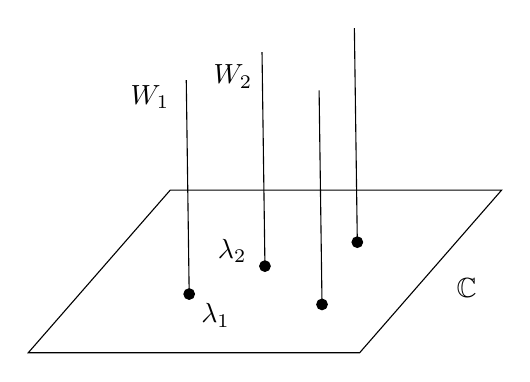
\begin{tikzpicture}[x=0.75pt,y=0.75pt,yscale=-1,xscale=1]
        %Shape: Parallelogram [id:dp548827135655336] 
        \draw   (129.38,106.55) -- (289.04,106.55) -- (220.61,184.94) -- (60.95,184.94) -- cycle ;
        %Shape: Circle [id:dp5536131887399003] 
        \draw  [color={rgb, 255:red, 0; green, 0; blue, 0 }  ,draw opacity=1 ][fill={rgb, 255:red, 0; green, 0; blue, 0 }  ,fill opacity=1 ] (135.95,156.64) .. controls (135.95,155.24) and (137.09,154.09) .. (138.5,154.09) .. controls (139.91,154.09) and (141.05,155.24) .. (141.05,156.64) .. controls (141.05,158.05) and (139.91,159.2) .. (138.5,159.2) .. controls (137.09,159.2) and (135.95,158.05) .. (135.95,156.64) -- cycle ;
        %Shape: Circle [id:dp3337454997914626] 
        \draw  [color={rgb, 255:red, 0; green, 0; blue, 0 }  ,draw opacity=1 ][fill={rgb, 255:red, 0; green, 0; blue, 0 }  ,fill opacity=1 ] (172.44,143.19) .. controls (172.44,141.78) and (173.59,140.64) .. (175,140.64) .. controls (176.4,140.64) and (177.55,141.78) .. (177.55,143.19) .. controls (177.55,144.6) and (176.4,145.74) .. (175,145.74) .. controls (173.59,145.74) and (172.44,144.6) .. (172.44,143.19) -- cycle ;
        %Shape: Circle [id:dp03436087376662322] 
        \draw  [color={rgb, 255:red, 0; green, 0; blue, 0 }  ,draw opacity=1 ][fill={rgb, 255:red, 0; green, 0; blue, 0 }  ,fill opacity=1 ] (199.95,161.64) .. controls (199.95,160.24) and (201.09,159.09) .. (202.5,159.09) .. controls (203.91,159.09) and (205.05,160.24) .. (205.05,161.64) .. controls (205.05,163.05) and (203.91,164.2) .. (202.5,164.2) .. controls (201.09,164.2) and (199.95,163.05) .. (199.95,161.64) -- cycle ;
        %Shape: Circle [id:dp09349939156591414] 
        \draw  [color={rgb, 255:red, 0; green, 0; blue, 0 }  ,draw opacity=1 ][fill={rgb, 255:red, 0; green, 0; blue, 0 }  ,fill opacity=1 ] (216.95,131.64) .. controls (216.95,130.24) and (218.09,129.09) .. (219.5,129.09) .. controls (220.91,129.09) and (222.05,130.24) .. (222.05,131.64) .. controls (222.05,133.05) and (220.91,134.2) .. (219.5,134.2) .. controls (218.09,134.2) and (216.95,133.05) .. (216.95,131.64) -- cycle ;
        %Straight Lines [id:da33322474104003263] 
        \draw    (137.09,53.57) -- (138.5,156.64) ;
        %Straight Lines [id:da7280355010137072] 
        \draw    (173.59,40.12) -- (175,143.19) ;
        %Straight Lines [id:da6839288750100709] 
        \draw    (201.09,58.57) -- (202.5,161.64) ;
        %Straight Lines [id:da9149673846486477] 
        \draw    (218.09,28.57) -- (219.5,131.64) ;
        
        % Text Node
        \draw (143.05,160.04) node [anchor=north west][inner sep=0.75pt]    {$\lambda _{1}$};
        % Text Node
        \draw (151.05,129.04) node [anchor=north west][inner sep=0.75pt]    {$\lambda _{2}$};
        % Text Node
        \draw (109.05,55.04) node [anchor=north west][inner sep=0.75pt]    {$W_{1}$};
        % Text Node
        \draw (149.05,45.04) node [anchor=north west][inner sep=0.75pt]    {$W_{2}$};
        % Text Node
        \draw (266.05,148.04) node [anchor=north west][inner sep=0.75pt]    {$\mathbb{C}$};
        
        
    \end{tikzpicture}
    \caption{The sheaf $\mathcal{F}_A \to \mathbb{C}$ of the linear operator $A: W \to W$. The support is the finite set $\text{Spec}(A) = \{\lambda_1, \dots, \lambda_m\}$. The stalk over $\lambda_i$ corresponds to the generalized eigenspace $W_i$.}
    \label{fig:figure5}
    \end{figure}
\begin{remark}
If $A$ is diagonalizable, $\mathcal{F}_A$ is a \textit{skyscraper sheaf}, supported only at the eigenvalues, with the stalk at $\lambda_i$ being the eigenspace $W_{\lambda_i}$. However, the decomposition \eqref{eq:4.8} depicted in Figure \ref{fig:figure5} does not determine the operator $A$ in general.

If there is a Jordan block of dimension $\alpha_i > 1$, the structure of the sheaf $\mathcal{F}_A$ in a formal (infinitesimal) neighborhood of the corresponding eigenvalue $\lambda_i$ encodes the nilpotent action $N = A - \lambda_i \text{id}_W$ on the generalized eigenspace $W_i$. This nilpotent structure, reflected in the flag \eqref{eq:4.6}, is captured by the non-trivial structure of the stalk $\mathcal{F}_{A,\lambda_i} \cong W_i$ as a module over the local ring $\mathcal{O}_{\C, \lambda_i}$ or its completion. The nilpotency is geometrically represented by this infinitesimal sheaf-theoretic behavior.
\end{remark}
\subsection{Projection-Valued Measures and Functional Calculus for Diagonalizable Operators}
\label{sec:pvm}

Henceforth in this section, we restrict our attention exclusively to linear operators $A: W \to W$ that are \textbf{diagonalizable} on a finite-dimensional complex vector space $W$. Recall that an operator $A$ is diagonalizable if and only if $W$ admits a basis consisting of eigenvectors of $A$, or equivalently, if its minimal polynomial has distinct roots. As we saw earlier, this is also equivalent to the geometric condition that the vector space $W$ decomposes as the direct sum of the eigenspaces of $A$. Let $\operatorname{Spec}(A) = \{\lambda_1, \dots, \lambda_m\} \subset \mathbb{C}$ denote the spectrum of $A$ (the set of distinct eigenvalues), and let $W_{\lambda_j} = \operatorname{Ker}(A - \lambda_j \operatorname{id}_W)$ be the eigenspace corresponding to the eigenvalue $\lambda_j$. By the definition of diagonalizability, the eigenspace decomposition provides an isomorphism:
\begin{equation*}
W \cong \bigoplus_{\lambda \in \operatorname{Spec}(A)} W_{\lambda}.
\end{equation*}
The action of the operator $A$ is completely determined by this decomposition and the associated eigenvalues: for any vector $w \in W$, if we decompose it uniquely as $w = \sum_{\lambda_j \in \operatorname{Spec}(A)} w_j$ with $w_j \in W_{\lambda_j}$, then $A(w) = \sum_{\lambda_j \in \operatorname{Spec}(A)} A(w_j) = \sum_{\lambda_j \in \operatorname{Spec}(A)} \lambda_j w_j$. Thus, $A$ simply acts as scalar multiplication by $\lambda_j$ on the subspace $W_{\lambda_j}$. This picture is captured by the interpretation of $A$ as the collection of its actions on the \dq{stalks} $W_\lambda$ over the discrete space $\operatorname{Spec}(A)$.

While intuitive, this description relies on the direct sum structure. We now develop an equivalent and powerful formalism that encodes such \dq{multiplication operators} purely in terms of projection operators associated with the eigenspaces. This projection-valued measure approach offers significant advantages, particularly for generalization.

\subsubsection{Projections, Orthogonal Projections, and Direct Sums}
\label{subsec:projections}

We begin by recalling and elaborating on the important properties of projection operators, which are the building blocks of spectral measures.

\begin{definition}[Projection Operator]
\label{def:projection_operator}
A linear operator $P: W \to W$ on a vector space $W$ is called a \textbf{projection} (or idempotent operator) if it satisfies the condition $P^2 = P$. The set of all projection operators on $W$ is denoted by $\operatorname{Proj}(W)$.
\end{definition}

Projections are linked to direct sum decompositions of the vector space.

\begin{proposition}[Projections and Direct Sums Correspondence]
\label{prop:proj_direct_sum}\,
\begin{enumerate}
    \item If $P \in \operatorname{Proj}(W)$, then $W$ decomposes as the direct sum of the image (range) and kernel (null space) of $P$:
        \begin{equation} \label{eq:4.12}
        W = \operatorname{Im}(P) \oplus \operatorname{Ker}(P).
        \end{equation}
        Furthermore, $P$ acts as the identity on $\operatorname{Im}(P)$ and as the zero operator on $\operatorname{Ker}(P)$. The operator $Q = \operatorname{id}_W - P$ is also a projection, called the complementary projection, satisfying $\operatorname{Im}(Q) = \operatorname{Ker}(P)$, $\operatorname{Ker}(Q) = \operatorname{Im}(P)$, and $PQ = QP = 0$.
    \item Conversely, given any direct sum decomposition $W = W'' \oplus W'$ into subspaces $W''$ and $W'$, there exists a unique projection operator $P: W \to W$ such that $\operatorname{Im}(P) = W''$ and $\operatorname{Ker}(P) = W'$. This operator is called the \textbf{projection onto $W''$ along $W'$}, and we denote it by $P''$. That is,
\begin{equation} \label{eq:4.13}
P'' : W \longrightarrow W, \quad \text{with } \operatorname{Im}(P'') = W'', \text{ and } \operatorname{Ker}(P'') = W'.
\end{equation}

\end{enumerate}
\end{proposition}
\begin{proof}\, 
    \begin{enumerate}
    \item For any $w \in W$, we can write
    \[
    w = Pw + (w - Pw).
    \]
    Clearly, $Pw \in \operatorname{Im}(P)$. Let $w' = w - Pw$. Then
    \[
    Pw' = P(w - Pw) = Pw - P^2w = Pw - Pw = 0,
    \]
    so $w' \in \operatorname{Ker}(P)$. This shows that
    \[
    W = \operatorname{Im}(P) + \operatorname{Ker}(P).
    \]
    To show the sum is direct, let $v \in \operatorname{Im}(P) \cap \operatorname{Ker}(P)$. Since $v \in \operatorname{Im}(P)$, there exists some $u \in W$ such that $v = Pu$. Since $v \in \operatorname{Ker}(P)$, we also have $Pv = 0$. Therefore,
    \[
    P^2u = 0,
    \]
    which implies $Pu = 0$, since $P^2 = P$. Hence, $v = 0$, proving the sum is direct.
    
    If $v \in \operatorname{Im}(P)$, then $v = Pu$, so $Pv = P^2u = Pu = v$. If $v \in \operatorname{Ker}(P)$, then $Pv = 0$.
    
    For $Q = \operatorname{id}_W - P$, we compute
    \[
    Q^2 = (\operatorname{id}_W - P)(\operatorname{id}_W - P) = \operatorname{id}_W - 2P + P^2 = \operatorname{id}_W - 2P + P = \operatorname{id}_W - P = Q.
    \]
    Thus, $Q^2 = Q$.
    
    Next, we find the kernel and image of $Q$:
    \[
    \operatorname{Ker}(Q) = \{w \mid (\operatorname{id}_W - P)w = 0\} = \{w \mid w = Pw\} = \operatorname{Im}(P),
    \]
    and
    \[
    \operatorname{Im}(Q) = \{(\operatorname{id}_W - P)w \mid w \in W\} = \operatorname{Ker}(P),
    \]
    as shown in the decomposition. Moreover, we have
    \[
    PQ = P(\operatorname{id}_W - P) = P - P^2 = 0,
    \]
    and
    \[
    QP = (\operatorname{id}_W - P)P = P - P^2 = 0.
    \]
    
    \item Given $W = W'' \oplus W'$, any $w \in W$ has a unique decomposition
    \[
    w = w'' + w',
    \]
    where $w'' \in W''$ and $w' \in W'$. Define $P(w) = w''$. This map is clearly linear. Its image is $W''$, and its kernel is
    \[
    \{w'' + w' \mid w'' = 0\} = W'.
    \]
    
    We now check idempotency:
    \[
    P^2(w) = P(w'') = w'' = P(w),
    \]
    since the decomposition of $w'' \in W''$ is $w'' = w'' + 0$.
    
    Uniqueness follows because any projection $P'$ with $\operatorname{Im}(P') = W''$ and $\operatorname{Ker}(P') = W'$ must map $w = w'' + w'$ to $P'(w'') + P'(w')$. Since $w'' \in \operatorname{Im}(P')$, we have $P'(w'') = w''$. Since $w' \in \operatorname{Ker}(P')$, we have $P'(w') = 0$. Thus,
    \[
    P'(w) = w'' = P(w).
    \]
\end{enumerate}
\end{proof}

When $W$ possesses an inner product structure $\langle \cdot, \cdot \rangle$, a special class of projections arises, characterized by compatibility with the inner product.

\begin{definition}[Orthogonal Projection]
\label{def:orthogonal_projection}
Let $(W, \langle \cdot, \cdot \rangle)$ be a finite-dimensional complex inner product space (i.e., a Hilbert space). A projection $P \in \operatorname{Proj}(W)$ is called an \textbf{orthogonal projection} if its image and kernel are orthogonal subspaces with respect to the inner product: $\operatorname{Im}(P) \perp \operatorname{Ker}(P)$. That is, $\langle Pw_1, (\operatorname{id}_W-P)w_2 \rangle = 0$ for all $w_1, w_2 \in W$.
\end{definition}

Orthogonal projections admit a important algebraic characterization involving the adjoint operator $P^*$, defined by $\langle Pw, v \rangle = \langle w, P^*v \rangle$ for all $v, w \in W$.

\begin{proposition}[Characterization of Orthogonal Projections]
\label{prop:orthog_proj_char}
A linear operator $P: W \to W$ on a finite-dimensional Hilbert space $W$ is an orthogonal projection if and only if it satisfies both $P^2 = P$ (idempotency) and $P^* = P$ (self-adjointness).
\end{proposition}
\begin{proof}
($\Rightarrow$) Assume that $P$ is an orthogonal projection. We already know that $P^2 = P$. We need to show that $P^* = P$. 

Since $W = \operatorname{Im}(P) \oplus \operatorname{Ker}(P)$ is an orthogonal decomposition, any $w, v \in W$ can be uniquely written as:
\[
w = w_1 + w_2 \quad \text{and} \quad v = v_1 + v_2,
\]
where $w_1, v_1 \in \operatorname{Im}(P)$ and $w_2, v_2 \in \operatorname{Ker}(P)$.

Therefore, we have:
\[
Pw = w_1 \quad \text{and} \quad Pv = v_1.
\]
We now compute the inner products:

\[
\langle Pw, v \rangle = \langle w_1, v_1 + v_2 \rangle = \langle w_1, v_1 \rangle + \langle w_1, v_2 \rangle = \langle w_1, v_1 \rangle,
\]
since $v_2 \in \operatorname{Ker}(P)$ and is orthogonal to $w_1 \in \operatorname{Im}(P)$.

Similarly:
\[
\langle w, Pv \rangle = \langle w_1 + w_2, v_1 \rangle = \langle w_1, v_1 \rangle + \langle w_2, v_1 \rangle = \langle w_1, v_1 \rangle,
\]
since $w_2 \in \operatorname{Ker}(P)$ and is orthogonal to $v_1 \in \operatorname{Im}(P)$.

Since we have:
\[
\langle Pw, v \rangle = \langle w, Pv \rangle \quad \text{for all} \quad w, v \in W,
\]
it follows that $P^* = P$.

($\Leftarrow$) Now assume that $P^2 = P$ and $P^* = P$. We know that $W = \operatorname{Im}(P) \oplus \operatorname{Ker}(P)$. Let $u \in \operatorname{Im}(P)$ and $v \in \operatorname{Ker}(P)$. We want to show that $\langle u, v \rangle = 0$.

Since $u \in \operatorname{Im}(P)$, we have $u = Pu$. Since $v \in \operatorname{Ker}(P)$, we have $Pv = 0$. Therefore:
\[
\langle u, v \rangle = \langle Pu, v \rangle = \langle u, P^*v \rangle \quad \text{(by the definition of adjoint)}.
\]
Since $P^* = P$, we obtain:
\[
\langle u, v \rangle = \langle u, Pv \rangle.
\]
Since $Pv = 0$, it follows that:
\[
\langle u, v \rangle = \langle u, 0 \rangle = 0.
\]
Thus, $\operatorname{Im}(P) \perp \operatorname{Ker}(P)$, and therefore, $P$ is an orthogonal projection.

\end{proof}

\subsubsection{Projection-Valued Measures (PVMs) for Diagonalizable Operators}
\label{subsec:pvm_def}

We now return to our setting of a diagonalizable operator $A: W \to W$ on a finite-dimensional complex vector space $W$, with the eigenspace decomposition $W = \bigoplus_{\lambda \in \operatorname{Spec}(A)} W_{\lambda}$. Let $\pi_{\lambda_j} \in \operatorname{Proj}(W)$ denote the unique projection onto the eigenspace $W_{\lambda_j}$ along the direct sum of the other eigenspaces $\bigoplus_{\lambda_k \neq \lambda_j} W_{\lambda_k}$. These individual projections satisfy important orthogonality relations.

\begin{lemma}[Properties of Eigenspace Projections]
\label{lemma:eig_proj_props}
Let $A$ be diagonalizable with distinct eigenvalues $\operatorname{Spec}(A) = \{\lambda_1, \dots, \lambda_m\}$, and let $\pi_{\lambda_j}$ be the projection onto $W_{\lambda_j}$ along $\bigoplus_{k \neq j} W_{\lambda_k}$. Then:
\begin{enumerate}
    \item $\sum_{j=1}^m \pi_{\lambda_j} = \operatorname{id}_W$ (Resolution of Identity).
    \item $\pi_{\lambda_j} \pi_{\lambda_k} = \delta_{jk} \pi_{\lambda_j}$ (Orthogonality of Projections).
\end{enumerate}
\end{lemma}
\begin{proof}\,

(1) Any $w \in W$ decomposes uniquely as $w = \sum_{k=1}^m w_k$ with $w_k \in W_{\lambda_k}$. By definition, $\pi_{\lambda_j}(w) = w_j$. Therefore, $(\sum_{j=1}^m \pi_{\lambda_j})(w) = \sum_{j=1}^m \pi_{\lambda_j}(w) = \sum_{j=1}^m w_j = w = \operatorname{id}_W(w)$. Since this holds for all $w$, $\sum \pi_{\lambda_j} = \operatorname{id}_W$.

(2) Consider $\pi_{\lambda_j} \pi_{\lambda_k}$. The image of $\pi_{\lambda_k}$ is $W_{\lambda_k}$. If $j \neq k$, then $W_{\lambda_k}$ is contained in the kernel of $\pi_{\lambda_j}$ (since $\operatorname{Ker}(\pi_{\lambda_j}) = \bigoplus_{l \neq j} W_{\lambda_l}$). Therefore, for $j \neq k$, $\pi_{\lambda_j} \pi_{\lambda_k} = 0$. If $j = k$, then $\pi_{\lambda_j} \pi_{\lambda_j} = (\pi_{\lambda_j})^2 = \pi_{\lambda_j}$ since $\pi_{\lambda_j}$ is a projection. Combining these, $\pi_{\lambda_j} \pi_{\lambda_k} = \delta_{jk} \pi_{\lambda_j}$.
\end{proof}

These projections allow us to define a set function whose values are operators, associating subsets of the complex plane to projections onto corresponding sums of eigenspaces.

\begin{definition}[Projection-Valued Measure (Finite-Dimensional Case)]
\label{def:pvm_finite}
Let $A: W \to W$ be a diagonalizable operator on a finite-dimensional complex vector space $W$. The \textbf{projection-valued measure (PVM)} or \textbf{spectral measure} associated with $A$ is the map
\begin{equation} \label{eq:4.14}
\pi_A : \mathcal{P}(\mathbb{C}) \longrightarrow \operatorname{Proj}(W)
\end{equation}
(where $\mathcal{P}(\mathbb{C})$ is the power set of $\mathbb{C}$) defined by assigning to each subset $E \subseteq \mathbb{C}$ the projection onto the sum of eigenspaces corresponding to eigenvalues lying within $E$:
\[ E \mapsto \pi_A(E) \coloneqq \sum_{\lambda_j \in E \cap \operatorname{Spec}(A)} \pi_{\lambda_j} \]
where $\pi_{\lambda_j}$ is the projection onto the eigenspace $W_{\lambda_j}$ along $\bigoplus_{k \neq j} W_{\lambda_k}$. If $E \cap \operatorname{Spec}(A)$ is empty, the sum is empty and defined as the zero operator.
\end{definition}

\begin{remark}[Dependence on Spectrum]
Observe that although the domain is formally written as $\mathcal{P}(\mathbb{C})$, the map $\pi_A$ is constant on sets $E$ having the same intersection with the finite set $\operatorname{Spec}(A)$. It is non-zero only for sets $E$ that contain at least one eigenvalue of $A$. Effectively, $\pi_A$ is supported on $\operatorname{Spec}(A)$.
\end{remark}

\begin{remark}[Orthogonality for Normal Operators]
\label{rem:pvm_normal}
If $W$ is equipped with an inner product $\langle \cdot, \cdot \rangle$ and the operator $A$ is \textbf{normal} (i.e., $A$ commutes with its adjoint, $AA^* = A^*A$), then $A$ is diagonalizable, and its eigenspaces corresponding to distinct eigenvalues are mutually orthogonal: $W_{\lambda_j} \perp W_{\lambda_k}$ for $j \neq k$. In this case, the direct sum $W = \bigoplus_{\lambda_j \in \operatorname{Spec}(A)} W_{\lambda_j}$ is an orthogonal direct sum. Consequently, each individual projection $\pi_{\lambda_j}$ is an orthogonal projection ($\pi_{\lambda_j}^* = \pi_{\lambda_j}$), and the PVM $\pi_A(E) = \sum_{\lambda_j \in E \cap \operatorname{Spec}(A)} \pi_{\lambda_j}$ is also an orthogonal projection for every $E \subseteq \mathbb{C}$. This holds, in particular, if $A$ is self-adjoint ($A^*=A$) or unitary ($A^*A = AA^* = \operatorname{id}_W$).
\end{remark}

The map $\pi_A$ exhibits properties strongly analogous to those of a classical (scalar-valued) measure, justifying its name.

\begin{proposition}[Properties of the PVM $\pi_A$]
\label{prop:pvm_props}
The map $\pi_A: \mathcal{P}(\mathbb{C}) \to \operatorname{Proj}(W)$ defined above satisfies the following properties:
\begin{itemize}
    \item[(i)] \textbf{Null Empty Set:} $\pi_A(\emptyset) = 0$.
    \item[(ii)] \textbf{Normalization:} $\pi_A(\mathbb{C}) = \pi_A(\operatorname{Spec}(A)) = \operatorname{id}_W$.
    \item[(iii)] \textbf{Finite Additivity:} If $E_1, E_2 \subseteq \mathbb{C}$ are disjoint subsets, then
        \[ \pi_A(E_1 \cup E_2) = \pi_A(E_1) + \pi_A(E_2). \]
        More generally, for pairwise disjoint $E_1, \dots, E_n$, $\pi_A(\cup_{i=1}^n E_i) = \sum_{i=1}^n \pi_A(E_i)$.
    \item[(iv)] \textbf{Multiplicativity/Intersection Property:} For any $E_1, E_2 \subseteq \mathbb{C}$,
        \[ \pi_A(E_1 \cap E_2) = \pi_A(E_1) \pi_A(E_2). \]
\end{itemize}
These properties imply, in particular, that projections associated with disjoint sets commute and their product is zero: if $E_1 \cap E_2 = \emptyset$, then $\pi_A(E_1) \pi_A(E_2) = \pi_A(E_1 \cap E_2) = \pi_A(\emptyset) = 0$.
\end{proposition}
\begin{proof}
Let $S = \operatorname{Spec}(A)$.

(i) $\pi_A(\emptyset) = \sum_{\lambda \in \emptyset \cap S} \pi_\lambda = 0$ (sum over empty set).

(ii) $\pi_A(\mathbb{C}) = \sum_{\lambda \in \mathbb{C} \cap S} \pi_\lambda = \sum_{\lambda \in S} \pi_\lambda = \operatorname{id}_W$ by Lemma \ref{lemma:eig_proj_props}(1). Similarly for $\pi_A(S)$.

(iii) If $E_1 \cap E_2 = \emptyset$, then $E_1 \cap S$ and $E_2 \cap S$ are disjoint subsets of $S$. The set of eigenvalues in the union is the disjoint union of the eigenvalues in each set: $(E_1 \cup E_2) \cap S = (E_1 \cap S) \cup (E_2 \cap S)$. Therefore,
    \[ \pi_A(E_1 \cup E_2) = \sum_{\lambda \in (E_1 \cup E_2) \cap S} \pi_\lambda = \sum_{\lambda \in (E_1 \cap S)} \pi_\lambda + \sum_{\lambda \in (E_2 \cap S)} \pi_\lambda = \pi_A(E_1) + \pi_A(E_2). \]

(iv) Using the definition and the orthogonality property $\pi_\lambda \pi_\mu = \delta_{\lambda\mu} \pi_\lambda$ from Lemma \ref{lemma:eig_proj_props}(2):
\begin{align*} \pi_A(E_1) \pi_A(E_2) &= \left( \sum_{\lambda \in E_1 \cap S} \pi_\lambda \right) \left( \sum_{\mu \in E_2 \cap S} \pi_\mu \right) \\ &= \sum_{\lambda \in E_1 \cap S} \sum_{\mu \in E_2 \cap S} \pi_\lambda \pi_\mu \\ &= \sum_{\lambda \in E_1 \cap S} \sum_{\mu \in E_2 \cap S} \delta_{\lambda\mu} \pi_\lambda \\ &= \sum_{\lambda \in (E_1 \cap S) \cap (E_2 \cap S)} \pi_\lambda \quad (\text{only terms with } \lambda=\mu \text{ survive}) \\ &= \sum_{\lambda \in (E_1 \cap E_2) \cap S} \pi_\lambda \\ &= \pi_A(E_1 \cap E_2). \qedhere \end{align*}
\end{proof}

The set of projections $\{\pi_{\lambda_j}\}_{\lambda_j \in \operatorname{Spec}(A)}$ associated with individual eigenvalues forms the core of the PVM. They constitute a complete set of mutually orthogonal (in the sense $\pi_j \pi_k = 0$ for $j \neq k$) projections summing to the identity, often called a \textbf{resolution of the identity} associated with $A$.

\subsubsection{Connection to Probability Measures}

The designation of the map $\pi_A : \mathcal{P}(\mathbb{C}) \longrightarrow \operatorname{Proj}(W)$ as a projection valued measure invites a comparison to the more familiar concept of classical, scalar-valued measures, particularly probability measures. While PVMs are operator-valued, their mathematical properties enable the construction of classical probability measures associated with vectors in the underlying space, thereby providing a general framework.

We first recall the basics of classical measure theory and probability spaces.

\begin{definition}[Measurable Space and $\sigma$-Algebra]
A \textbf{measurable space} is a pair $(X, \Sigma)$, where $X$ is a non-empty set, often called the \dq{sample space} or \dq{universe of outcomes,} and $\Sigma$ is a \textbf{$\sigma$-algebra} (or $\sigma$-field) of subsets of $X$. $\Sigma$ is a collection of subsets of $X$ satisfying:
\begin{enumerate}
    \item $X \in \Sigma$ (the entire space is measurable).
    \item If $E \in \Sigma$, then its complement $X \setminus E$ is also in $\Sigma$ (closure under complementation).
    \item If $\{E_i\}_{i=1}^\infty$ is a countable collection of sets in $\Sigma$, then their union $\cup_{i=1}^\infty E_i$ is in $\Sigma$ (closure under countable unions).
\end{enumerate}
The elements of $\Sigma$ are called \dq{measurable sets} or, in probabilistic contexts, \dq{events.}
\end{definition}

\begin{definition}[Positive Measure]
A \textbf{positive measure} on a measurable space $(X, \Sigma)$ is a function $\mu: \Sigma \to [0, \infty]$ (the set of non-negative extended real numbers) such that:
\begin{enumerate}
    \item $\mu(\emptyset) = 0$ (the measure of the empty set is zero).
    \item (Countable Additivity / $\sigma$-additivity) For any countable sequence $\{E_i\}_{i=1}^\infty$ of pairwise disjoint sets in $\Sigma$ (i.e., $E_i \cap E_j = \emptyset$ for $i \neq j$),
        \[ \mu\left(\bigcup_{i=1}^\infty E_i\right) = \sum_{i=1}^\infty \mu(E_i). \]
\end{enumerate}
\end{definition}
From these axioms, several standard properties of measures follow, including:
\begin{itemize}
    \item Finite Additivity: For any finite collection of pairwise disjoint sets $E_1, \dots, E_n \in \Sigma$, $\mu(\cup_{k=1}^n E_k) = \sum_{k=1}^n \mu(E_k)$.
    \item Monotonicity: If $E, F \in \Sigma$ and $E \subseteq F$, then $\mu(E) \le \mu(F)$.
    \item Subadditivity: For any countable collection $\{E_i\}_{i=1}^\infty$ of sets in $\Sigma$ (not necessarily disjoint), $\mu(\cup_{i=1}^\infty E_i) \le \sum_{i=1}^\infty \mu(E_i)$.
    \item Continuity from below: If $E_1 \subseteq E_2 \subseteq \dots$ is an increasing sequence of sets in $\Sigma$ and $E = \cup_{n=1}^\infty E_n$, then $\mu(E) = \lim_{n\to\infty} \mu(E_n)$.
    \item Continuity from above: If $E_1 \supseteq E_2 \supseteq \dots$ is a decreasing sequence of sets in $\Sigma$, $E = \cap_{n=1}^\infty E_n$, and $\mu(E_1) < \infty$, then $\mu(E) = \lim_{n\to\infty} \mu(E_n)$.
\end{itemize}

\begin{definition}[Finite Measures and Probability Measures]\,
\begin{enumerate}
    \item A positive measure $\mu$ is \textbf{finite} if $\mu(X) < \infty$.
    \item A positive measure $P$ on $(X, \Sigma)$ is a \textbf{probability measure} if $P(X) = 1$. The triple $(X, \Sigma, P)$ is then termed a \textbf{probability space}.
\end{enumerate}
More generally, one defines signed measures (real-valued) and complex measures, both satisfying countable additivity.
\end{definition}
In the context of a PVM $\pi_A$ for a diagonalizable operator $A$ on a finite-dimensional space $W$, the spectrum $\operatorname{Spec}(A)$ is a finite set. We can take $X = \operatorname{Spec}(A)$ and $\Sigma = \mathcal{P}(\operatorname{Spec}(A))$ (the power set of the spectrum). In this scenario, any finitely additive set function automatically satisfies countable additivity because any countable disjoint union can only contain finitely many non-empty sets.

The PVM $\pi_A$, as defined in Definition \ref{def:pvm_finite} has many parallels to the axiomatic structure of a probability measure, especially concerning its behavior under set operations (Proposition \ref{prop:pvm_props}).

\begin{itemize}
    \item[(i)] \textbf{Null Empty Set: $\pi_A(\emptyset) = 0$.}
    This is structurally identical to $P(\emptyset)=0$. The PVM assigns the zero operator to the empty set of spectral values, signifying that the \dq{spectral content} associated with no eigenvalues is trivial (projection onto the zero-dimensional subspace $\{0_W\}$).

    \item[(ii)] \textbf{Normalization / Total Measure: $\pi_A(\mathbb{C}) = \pi_A(\operatorname{Spec}(A)) = \operatorname{id}_W$.}
    This parallels $P(X)=1$. The identity operator $\operatorname{id}_W$ serves as the operatorial analogue of \dq{total probability} or \dq{certainty.} It confirms that the entire space $W$ is accounted for by the spectral decomposition $W = \bigoplus_{\lambda \in \operatorname{Spec}(A)} W_{\lambda}$. The sum of projections onto all distinct eigenspaces, $\sum_{\lambda \in \operatorname{Spec}(A)} \pi_\lambda = \operatorname{id}_W$ (see Lemma \ref{lemma:eig_proj_props}).

    \item[(iii)] \textbf{Finite Additivity: $\pi_A(E_1 \cup E_2) = \pi_A(E_1) + \pi_A(E_2)$ for disjoint $E_1, E_2 \subseteq \mathbb{C}$.}
    This mirrors the additivity $P(E_1 \cup E_2) = P(E_1) + P(E_2)$ for mutually exclusive events. The PVM property follows from its definition as a sum over individual eigenspace projections:
    \[ \pi_A(E_1 \cup E_2) = \sum_{\lambda \in (E_1 \cap S) \cup (E_2 \cap S)} \pi_\lambda = \sum_{\lambda \in E_1 \cap S} \pi_\lambda + \sum_{\lambda \in E_2 \cap S} \pi_\lambda = \pi_A(E_1) + \pi_A(E_2), \]
    where $S = \operatorname{Spec}(A)$ and the disjointness of $E_1, E_2$ implies disjointness of $E_1 \cap S$ and $E_2 \cap S$. The sum is one of linear operators. For this sum $\pi_A(E_1) + \pi_A(E_2)$ to itself be a projection (which $\pi_A(E_1 \cup E_2)$ is), a necessary and sufficient condition is that $\pi_A(E_1)\pi_A(E_2) = 0$ and $\pi_A(E_2)\pi_A(E_1) = 0$. This condition is indeed satisfied due to property (iv) below, as $E_1 \cap E_2 = \emptyset \implies \pi_A(E_1)\pi_A(E_2) = \pi_A(\emptyset) = 0$. The image of $\pi_A(E_1 \cup E_2)$ is then the direct sum of the images of $\pi_A(E_1)$ and $\pi_A(E_2)$.
\end{itemize}

The major difference from classical probability measures is that $\pi_A(E)$ is an operator (a projection) and not a scalar value in $[0,1]$. However, this operator-valued structure provides a way to generate classical scalar measures, including probability measures, when an inner product and specific vectors (states) are introduced. This is particularly transparent for normal operators, where the PVM consists of orthogonal projections.

Let $W$ be a finite-dimensional complex inner product space, and let $A$ be a normal operator on $W$. Then its PVM $\pi_A(E)$ consists of orthogonal projections (i.e., $\pi_A(E)^* = \pi_A(E)$ and $\pi_A(E)^2 = \pi_A(E)$). For any vector $\psi \in W$, consider the map $\mu_\psi: \mathcal{P}(\operatorname{Spec}(A)) \to [0, \infty)$ defined by:
\[ \mu_\psi(E) \coloneqq \langle \psi, \pi_A(E)\psi \rangle. \]
Since $\pi_A(E)$ is an orthogonal projection, 
\begin{align*}
    \langle \psi, \pi_A(E)\psi \rangle &= \langle \psi, \pi_A(E)^*\pi_A(E)\psi \rangle \\ 
    &= \langle \pi_A(E)\psi, \pi_A(E)\psi \rangle \\ 
    &= \|\pi_A(E)\psi\|^2 \ge 0.
\end{align*}
This map $\mu_\psi$ is a finite positive measure on $\operatorname{Spec}(A)$:
\begin{enumerate}
    \item $\mu_\psi(\emptyset) = \|\pi_A(\emptyset)\psi\|^2 = \|0\psi\|^2 = 0$.
    \item (Finite Additivity) For disjoint $E_1, E_2 \subseteq \operatorname{Spec}(A)$:
    The projections $\pi_A(E_1)$ and $\pi_A(E_2)$ are orthogonal and their images are orthogonal subspaces because $E_1 \cap E_2 = \emptyset \implies \pi_A(E_1)\pi_A(E_2)=0$. This means that $\pi_A(E_1)\psi$ is orthogonal to $\pi_A(E_2)\psi$.
    Thus,
    \begin{align*} \mu_\psi(E_1 \cup E_2) &= \|\pi_A(E_1 \cup E_2)\psi\|^2 = \|(\pi_A(E_1) + \pi_A(E_2))\psi\|^2 \\ &= \|\pi_A(E_1)\psi + \pi_A(E_2)\psi\|^2 \\ &= \|\pi_A(E_1)\psi\|^2 + \|\pi_A(E_2)\psi\|^2 \quad (\text{by the Pythagorean theorem}) \\ &= \mu_\psi(E_1) + \mu_\psi(E_2). \end{align*}
\end{enumerate}
The total measure is $\mu_\psi(\operatorname{Spec}(A)) = \|\pi_A(\operatorname{Spec}(A))\psi\|^2 = \|\operatorname{id}_W \psi\|^2 = \|\psi\|^2$.
Crucially, if the vector $\psi$ is normalized such that $\|\psi\|=1$, then $\mu_\psi(\operatorname{Spec}(A)) = 1$. In this case, $\mu_\psi$ becomes a classical \textbf{probability measure} on the finite set $\operatorname{Spec}(A)$. Thus, the PVM $\pi_A$, while operator-valued, naturally induces a family of probability measures, parameterized by the choice of a normalized vector $\psi$. Each such $\mu_\psi$ describes a probability distribution over the possible spectral values of $A$.

More generally, for any pair of vectors $\phi, \psi \in W$, the function $\mu_{\phi,\psi}(E) \coloneqq \langle \phi, \pi_A(E)\psi \rangle$ defines a complex measure on $\operatorname{Spec}(A)$. These are essential for defining the integral $\langle \phi, f(A)\psi \rangle = \int f(\lambda)d\mu_{\phi,\psi}(\lambda)$ for complex-valued functions $f$.

Once we have the probability measure $\mu_\psi$ associated with a normalized vector $\psi$ and a self-adjoint operator $A$ (whose spectrum is real), we can define the expectation of a function $f: \operatorname{Spec}(A) \to \mathbb{R}$ in the classical sense:
\[ \mathbb{E}_{\mu_\psi}[f] \coloneqq \int_{\operatorname{Spec}(A)} f(\lambda) \, d\mu_\psi(\lambda) = \sum_{\lambda_j \in \operatorname{Spec}(A)} f(\lambda_j) \mu_\psi(\{\lambda_j\}). \]
Using the functional calculus $f(A) = \sum_{\lambda_j \in \operatorname{Spec}(A)} f(\lambda_j) \pi_{\lambda_j}$ and $\mu_\psi(\{\lambda_j\}) = \langle \psi, \pi_{\lambda_j}\psi \rangle = \|\pi_{\lambda_j}\psi\|^2$, we find:
\begin{align*} \langle \psi, f(A)\psi \rangle &= \left\langle \psi, \sum_{\lambda_j \in \operatorname{Spec}(A)} f(\lambda_j) \pi_{\lambda_j} \psi \right\rangle \\ &= \sum_{\lambda_j \in \operatorname{Spec}(A)} f(\lambda_j) \langle \psi, \pi_{\lambda_j} \psi \rangle \\ &= \sum_{\lambda_j \in \operatorname{Spec}(A)} f(\lambda_j) \mu_\psi(\{\lambda_j\}) \\ &= \mathbb{E}_{\mu_\psi}[f]. \end{align*}
In particular, for $f(\lambda) = \lambda$, the \dq{average value} $\langle \psi, A\psi \rangle$ is precisely the expectation $\mathbb{E}_{\mu_\psi}[\lambda]$, where $\lambda$ is viewed as a random variable distributed according to $\mu_\psi$. Similarly, the variance can be defined:
\[ \operatorname{Var}_{\mu_\psi}(\lambda) = \mathbb{E}_{\mu_\psi}[(\lambda - \mathbb{E}_{\mu_\psi}[\lambda])^2] = \langle \psi, (A - \langle \psi, A\psi \rangle \operatorname{id}_W)^2 \psi \rangle. \]
This shows how the operatorial PVM framework connects directly to classical statistical concepts through the vector-dependent probability measures.

The PVM property (iv) $\pi_A(E_1 \cap E_2) = \pi_A(E_1) \pi_A(E_2)$ is another major difference from the properties of typical probability measures. For probabilities, $P(E_1 \cap E_2) = P(E_1)P(E_2)$ holds if and only if the events $E_1$ and $E_2$ are \textbf{statistically independent}. Independence is a specific relationship between events contingent on a particular probability measure $P$, not an axiom of probability measures themselves.

In contrast, for a PVM $\pi_A$ derived from a single operator $A$, the multiplicative property $\pi_A(E_1 \cap E_2) = \pi_A(E_1)\pi_A(E_2)$ is an inherent structural property. It follows from the idempotency and mutual orthogonality of the elementary spectral projections $\pi_\lambda \pi_\mu = \delta_{\lambda\mu}\pi_\lambda$. Since all $\pi_A(E)$ are sums of these $\pi_\lambda$, they all commute: $\pi_A(E_1)\pi_A(E_2) = \pi_A(E_2)\pi_A(E_1)$. This commutativity of projection values for any two sets is a key feature. The property reflects the underlying logic of spectral decomposition: applying a \dq{filter} for eigenvalues in $E_2$ and then a \dq{filter} for eigenvalues in $E_1$ is equivalent to applying a single \dq{filter} for eigenvalues in $E_1 \cap E_2$. This robust algebraic property is essential for ensuring that the functional calculus $f \mapsto f(A)$ defines an algebra homomorphism (specifically, $(fg)(A)=f(A)g(A)$).

The true power of this measure-theoretic perspective, especially its connection to probability, becomes fully apparent in the context of infinite-dimensional Hilbert spaces and operators with continuous spectra (as discussed in Section \ref{sec:hilbert}).
\begin{enumerate}
    \item The PVM $\pi_A$ associated with a self-adjoint operator $A$ is defined on the Borel $\sigma$-algebra $\mathcal{B}(\sigma(A))$ of its spectrum.
    \item The crucial property is \textbf{countable additivity (strong operator topology-convergence)}: for any sequence $\{E_i\}_{i=1}^\infty$ of pairwise disjoint Borel sets,
        \[ \pi_A\left(\bigcup_{i=1}^\infty E_i\right)\psi = \sum_{i=1}^\infty \pi_A(E_i)\psi \quad (\text{for all } \psi \in \mathcal{H}). \]
\end{enumerate}
This SOT-countable additivity of the PVM $\pi_A$ is precisely the condition required to ensure that each derived scalar function $\mu_\psi(E) = \|\pi_A(E)\psi\|^2$ is a true, countably additive probability measure on $(\sigma(A), \mathcal{B}(\sigma(A)))$ when $\|\psi\|=1$. This mathematical structure supports the probabilistic interpretation of quantum measurements, even for observables with continuous spectra like position or momentum, where sums turn into integrals against probability measures determined by the quantum state.

To summarize, while PVMs are fundamentally operator-valued, they share core axiomatic traits with scalar measures, particularly concerning normalization and additivity for disjoint sets. For normal operators on an inner product space, the PVM, being composed of orthogonal projections, naturally allows the construction of a family of classical positive scalar measures $\mu_\psi(E) = \|\pi_A(E)\psi\|^2$. When the vector $\psi$ is normalized, $\mu_\psi$ becomes a probability measure on the spectrum of $A$. This provides a purely mathematical pathway to probabilistic interpretations. The expectation values formed with respect to these probability measures align perfectly with the inner product expressions like $\langle \psi, f(A)\psi \rangle$. The distinctive multiplicative property of PVMs, $\pi_A(E_1 \cap E_2) = \pi_A(E_1)\pi_A(E_2)$, is an algebraic feature that has no direct counterpart in general probability theory beyond the special case of statistical independence; for PVMs, it is important for the homomorphism property of the functional calculus. Overall, PVMs offer a mathematical framework in which operator-valued measures can produce classical probability distributions when applied to specific states.

\subsubsection{The Functional Calculus for Diagonalizable Operators}
\label{subsec:functional_calculus_finite}

The primary purpose of the PVM formalism is to provide a unified way to define functions of the operator $A$. This is known as the functional calculus. Applying functions to operators naturally arises in various contexts, such as solving systems of linear differential equations ($e^{tA}$), defining norms or condition numbers of matrices, and formulating observables and their evolution in quantum mechanics.

First, the operator $A$ itself can be reconstructed from its eigenvalues and the corresponding projections. Since $A$ acts as $\lambda_j \operatorname{id}_{W_{\lambda_j}}$ on the image of $\pi_{\lambda_j}$, and $\sum \pi_{\lambda_j} = \operatorname{id}_W$, we can write $A$ as a linear combination of these projections, weighted by the eigenvalues.

\begin{proposition}[Spectral Decomposition of A]
\label{prop:spectral_decomp}
Let $A$ be a diagonalizable operator with distinct eigenvalues $\operatorname{Spec}(A) = \{\lambda_1, \dots, \lambda_m\}$ and corresponding eigenspace projections $\pi_{\lambda_j}$. Then $A$ can be expressed as:
\begin{equation} \label{eq:4.15}
A = \sum_{j=1}^m \lambda_j \pi_{\lambda_j}.
\end{equation}
This is often written suggestively as an integral with respect to the PVM:
\[ A = \int_{\mathbb{C}} \lambda \, d\pi_A(\lambda) \quad \text{or} \quad A = \int_{\operatorname{Spec}(A)} \lambda \, d\pi_A(\lambda). \]
\end{proposition}
\begin{proof}
    Let $w \in W$. Decompose $w = \sum_{k=1}^m w_k$ where 
    \[
    w_k = \pi_{\lambda_k}(w) \in W_{\lambda_k}.
    \]
    Then 
    \[
    A(w) = \sum_{k=1}^m A(w_k) = \sum_{k=1}^m \lambda_k w_k.
    \]
    Now compute the action of the sum:
    \[
    \left( \sum_{j=1}^m \lambda_j \pi_{\lambda_j} \right)(w) = \sum_{j=1}^m \lambda_j \pi_{\lambda_j} \left( \sum_{k=1}^m w_k \right) = \sum_{j=1}^m \sum_{k=1}^m \lambda_j \pi_{\lambda_j} w_k.
    \]
    Since $w_k \in W_{\lambda_k}$, we have
    \[
    \pi_{\lambda_j} w_k = \delta_{jk} w_k.
    \]
    Thus, the sum becomes
    \[
    \sum_{j=1}^m \sum_{k=1}^m \lambda_j \delta_{jk} w_k = \sum_{k=1}^m \lambda_k w_k.
    \]
    This equals $A(w)$. Since the operators agree on all $w$, they are equal. The integral notation emphasizes that $A$ is synthesized from its spectral values $\lambda$ weighted by the spectral measure $\pi_A$ concentrated at those values.
    
\end{proof}

This spectral decomposition naturally suggests how to define $f(A)$ for functions $f$. If $p(z) = \sum_{k=0}^N c_k z^k$ is a polynomial, then using $A^k = (\sum \lambda_j \pi_{\lambda_j})^k = \sum \lambda_j^k \pi_{\lambda_j}$ (due to $\pi_j \pi_l = \delta_{jl} \pi_j$), we find
\[ p(A) = \sum_{k=0}^N c_k A^k = \sum_{k=0}^N c_k \left( \sum_{j=1}^m \lambda_j^k \pi_{\lambda_j} \right) = \sum_{j=1}^m \left( \sum_{k=0}^N c_k \lambda_j^k \right) \pi_{\lambda_j} = \sum_{j=1}^m p(\lambda_j) \pi_{\lambda_j}. \]
This calculation shows that applying a polynomial $p$ to the operator $A$ is equivalent to applying $p$ to each eigenvalue $\lambda_j$ and summing the results weighted by the corresponding projection $\pi_{\lambda_j}$. This motivates extending the definition from polynomials to arbitrary functions defined on the spectrum of $A$.

\begin{definition}[Functional Calculus]
\label{def:functional_calculus}
Let $A: W \to W$ be a diagonalizable operator with spectral measure $\pi_A$. Let $f: \operatorname{Spec}(A) \to \mathbb{C}$ be any function defined on the spectrum of $A$. (We can extend $f$ to all of $\mathbb{C}$ arbitrarily, e.g., by setting $f(\lambda)=0$ for $\lambda \notin \operatorname{Spec}(A)$, as only its values on $\operatorname{Spec}(A)$ affect the sum). The operator $f(A): W \to W$ is defined as:
\begin{equation} \label{eq:4.16}
f(A) \coloneqq \sum_{\lambda_j \in \operatorname{Spec}(A)} f(\lambda_j) \pi_{\lambda_j}.
\end{equation}
This can also be written using the integral notation:
\[ f(A) = \int_{\operatorname{Spec}(A)} f(\lambda) \, d\pi_A(\lambda). \]
This map $f \mapsto f(A)$ is called the \textbf{functional calculus} for the diagonalizable operator $A$.
\end{definition}

This definition provides a consistent and computationally effective way to apply functions to operators.
\begin{example}[Applying Functions to Functional Calculus]\,
\begin{itemize}
    \item The operator exponential $e^{tA}$ (important for solving linear ODE systems $\dot{x}=Ax$) is given by 
    \[e^{tA} = \sum_{j=1}^m e^{t\lambda_j} \pi_{\lambda_j}.\]
    \item If $0 \notin \operatorname{Spec}(A)$, meaning $A$ is invertible, we can define $f(\lambda) = 1/\lambda$ for $\lambda \in \operatorname{Spec}(A)$. Then the inverse is 
    \[A^{-1} = f(A) = \sum_{j=1}^m \frac{1}{\lambda_j} \pi_{\lambda_j}.\] 
    We can verify this: 
    \[A A^{-1} = (\sum_{k=1}^m \lambda_k \pi_{\lambda_k})(\sum_{j=1}^m \frac{1}{\lambda_j} \pi_{\lambda_j}) = \sum_{j,k=1}^m \frac{\lambda_k}{\lambda_j} \pi_{\lambda_k} \pi_{\lambda_j} = \sum_{j=1}^m \frac{\lambda_j}{\lambda_j} \pi_{\lambda_j} = \sum_{j=1}^m \pi_{\lambda_j} = \operatorname{id}_W.\]
    \item Consider the matrix $A = \begin{pmatrix} 2 & 0 \\ 0 & -1 \end{pmatrix}$. The spectrum of $A$ is given by 
    \[
    \operatorname{Spec}(A) = \{2, -1\}.
    \]
    Let 
    \[
    W_2 = \operatorname{span}\left\{ \begin{pmatrix} 1 \\ 0 \end{pmatrix} \right\}, \quad W_{-1} = \operatorname{span}\left\{ \begin{pmatrix} 0 \\ 1 \end{pmatrix} \right\}.
    \]
    The corresponding projection operators are
    \[
    \pi_2 = \begin{pmatrix} 1 & 0 \\ 0 & 0 \end{pmatrix}, \quad \pi_{-1} = \begin{pmatrix} 0 & 0 \\ 0 & 1 \end{pmatrix}.
    \]
    
    Now, let $f(x) = x^3$. We can compute $f(A)$ as follows:
    \[
    f(A) = f(2)\pi_2 + f(-1)\pi_{-1} = 8\pi_2 + (-1)\pi_{-1} = \begin{pmatrix} 8 & 0 \\ 0 & -1 \end{pmatrix},
    \]
    which is equal to $A^3$.
    
    Next, let $g(x) = \sqrt{x}$ (defined for positive eigenvalues). If 
    \[
    A = \begin{pmatrix} 4 & 0 \\ 0 & 9 \end{pmatrix},
    \]
    then we compute $g(A)$ as follows:
    \[
    g(A) = \sqrt{4}\pi_4 + \sqrt{9}\pi_9 = 2\pi_4 + 3\pi_9 = \begin{pmatrix} 2 & 0 \\ 0 & 3 \end{pmatrix},
    \]
    which is one possible square root of $A$.
\end{itemize}
\end{example}

The functional calculus possesses important algebraic properties, formalizing the idea that calculations with $f(A)$ mirror calculations with the function $f$ itself on the spectrum. Let $\mathcal{F}(\operatorname{Spec}(A))$ be the algebra of complex-valued functions on the finite set $\operatorname{Spec}(A)$ equipped with pointwise addition, scalar multiplication, and pointwise multiplication. Let $\mathcal{L}(W)$ be the algebra of linear operators on $W$.

\begin{theorem}[Properties of the Functional Calculus]
\label{thm:func_calc_props}
The functional calculus map $\Psi: \mathcal{F}(\operatorname{Spec}(A)) \to \mathcal{L}(W)$ defined by $\Psi(f) = f(A)$ is an algebra homomorphism. That is, for $f, g \in \mathcal{F}(\operatorname{Spec}(A))$ and $c \in \mathbb{C}$:
\begin{enumerate}
    \item $\Psi(f+g) = (f+g)(A) = f(A) + g(A) = \Psi(f) + \Psi(g)$ (Additivity).
    \item $\Psi(cf) = (cf)(A) = c f(A) = c \Psi(f)$ (Homogeneity).
    \item $\Psi(fg) = (fg)(A) = f(A) g(A) = \Psi(f) \Psi(g)$ (Multiplicativity).
    \item $\Psi(\mathbf{1}) = \mathbf{1}(A) = \operatorname{id}_W$, where $\mathbf{1}$ is the constant function $f(\lambda)=1$.
    \item $\Psi(\mathrm{id}_{\mathbb{C}}) = \mathrm{id}_{\mathbb{C}}(A) = A$, where $\mathrm{id}_{\mathbb{C}}$ is the identity function $f(\lambda)=\lambda$.
\end{enumerate}
If $W$ is equipped with an inner product and $A$ is a normal operator, then $\Psi$ is furthermore a *-homomorphism, meaning it respects the adjoint operation (involution):
\begin{enumerate}
    \item[6.] $\Psi(\bar{f}) = \bar{f}(A) = (f(A))^* = (\Psi(f))^*$, where $\bar{f}$ is the complex conjugate function $\bar{f}(\lambda) = \overline{f(\lambda)}$.
\end{enumerate}
\end{theorem}
\begin{proof}
Properties (1) and (2) follow directly from the linearity of the summation in the definition \eqref{eq:4.16}:
\begin{align*}
    (f+g)(A) &= \sum (f+g)(\lambda_j) \pi_j\\ 
    &= \sum (f(\lambda_j)+g(\lambda_j)) \pi_j \\ 
    &= \sum f(\lambda_j)\pi_j + \sum g(\lambda_j)\pi_j \\ 
    &= f(A)+g(A)
\end{align*}
and
\begin{align*}
    (cf)(A) &= \sum (cf)(\lambda_j) \pi_j \\
    &= \sum c f(\lambda_j) \pi_j \\ 
    &= c \sum f(\lambda_j)\pi_j \\
    &= c f(A).
\end{align*}

(3) Multiplicativity:
\begin{align*} f(A) g(A) &= \left( \sum_{j=1}^m f(\lambda_j) \pi_{\lambda_j} \right) \left( \sum_{k=1}^m g(\lambda_k) \pi_{\lambda_k} \right) \\ &= \sum_{j,k=1}^m f(\lambda_j) g(\lambda_k) (\pi_{\lambda_j} \pi_{\lambda_k}) \\ &= \sum_{j,k=1}^m f(\lambda_j) g(\lambda_k) (\delta_{jk} \pi_{\lambda_j}) \quad (\text{using Lemma \ref{lemma:eig_proj_props}(2)}) \\ &= \sum_{j=1}^m f(\lambda_j) g(\lambda_j) \pi_{\lambda_j} \\ &= \sum_{j=1}^m (fg)(\lambda_j) \pi_{\lambda_j} = (fg)(A). \end{align*}
(4) $\mathbf{1}(A) = \sum \mathbf{1}(\lambda_j) \pi_{\lambda_j} = \sum 1 \cdot \pi_{\lambda_j} = \operatorname{id}_W$ by Lemma \ref{lemma:eig_proj_props}(1).
(5) $\mathrm{id}_{\mathbb{C}}(A) = \sum \mathrm{id}_{\mathbb{C}}(\lambda_j) \pi_{\lambda_j} = \sum \lambda_j \pi_{\lambda_j} = A$ by Proposition \ref{prop:spectral_decomp}.
(6) Assume $W$ is a Hilbert space and $A$ is normal. Then each $\pi_{\lambda_j}$ is an orthogonal projection, so $\pi_{\lambda_j}^* = \pi_{\lambda_j}$ by Proposition \ref{prop:orthog_proj_char} and Remark \ref{rem:pvm_normal}. The adjoint of a sum is the sum of adjoints, and the adjoint of a scalar multiple is the conjugate scalar multiple of the adjoint:
\begin{align*} (f(A))^* &= \left( \sum_{j=1}^m f(\lambda_j) \pi_{\lambda_j} \right)^* \\ &= \sum_{j=1}^m \overline{f(\lambda_j)} (\pi_{\lambda_j})^* \quad (\text{properties of Hilbert space adjoint}) \\ &= \sum_{j=1}^m \overline{f(\lambda_j)} \pi_{\lambda_j} \quad (\text{since } \pi_{\lambda_j}^* = \pi_{\lambda_j}) \\ &= \sum_{j=1}^m \bar{f}(\lambda_j) \pi_{\lambda_j} = \bar{f}(A). \qedhere \end{align*}
\end{proof}

\subsection{Generalizations and Special Cases in Finite Dimensions}
\label{sec:special_cases_finite}

So far, we've seen how the framework of projection-valued measures provides a powerful, basis-independent, and elegant way to understand diagonalizable operators on finite-di\-men\-si\-o\-nal vector spaces. By shifting focus from eigenvectors to projections onto eigenspaces, we obtain a spectral measure $\pi_A$ supported on the spectrum $\operatorname{Spec}(A)$. This measure satisfies properties analogous to classical measures but takes values in the space of projection operators. The resolution of identity, $\sum \pi_{\lambda_j} = \operatorname{id}_W$, allows the reconstruction of the operator itself via its spectral decomposition, $A = \sum \lambda_j \pi_{\lambda_j}$.

This decomposition, in turn, forms the foundation for functional calculus, $f \mapsto f(A) = \sum f(\lambda_j) \pi_{\lambda_j}$. This calculus allows the application of arbitrary functions (defined on the spectrum) to the operator $A$ in a manner consistent with polynomial functions and respecting the algebraic structure (as formalized by the homomorphism properties in Theorem \ref{thm:func_calc_props}). When dealing with normal operators on Hilbert spaces, the PVM consists of orthogonal projections, and the functional calculus further respects the adjoint operation, making it a *-homomorphism.

While developed here for simplicity in finite dimensions, the true significance of the projection-valued measure and functional calculus perspective lies in its generalization to infinite-dimensional Hilbert spaces. The Spectral Theorem extends this framework to normal operators (bounded or unbounded). It asserts the existence of a PVM $\pi_A$ defined on the Borel $\sigma$-algebra of $\mathbb{C}$ (supported on the spectrum $\sigma(A)$, which may now be continuous) satisfying countable additivity, such that the operator and functions of it can be represented as integrals:
\[ A = \int_{\sigma(A)} \lambda \, d\pi_A(\lambda) \quad \text{and} \quad f(A) = \int_{\sigma(A)} f(\lambda) \, d\pi_A(\lambda). \]
This infinite-dimensional spectral theory is very valuable for quantum mechanics, where observables are modeled by self-adjoint operators $A$. The spectral measure $\pi_A$ then dictates the possible outcomes of measurements (the spectrum $\sigma(A)$) and their probabilities (via $\langle \psi, \pi_A(E) \psi \rangle$ for a state $\psi$ and outcome range $E$). The finite-dimensional theory, therefore, serves as an essential conceptual launchpad for understanding these deeper and more widely applicable results.

So far, we've seen the theory for a single diagonalizable operator. Now, we explore how to deal with families of operators that can be simultaneously diagonalizable, which is important for analyzing systems with multiple commuting observables or symmetries. This section explores these important specializations and generalizations within the finite-dimensional complex inner product space setting, laying essential groundwork for infinite-dimensional spectral theory and applications in quantum mechanics.

Throughout this section, unless otherwise specified, $W$ denotes a finite-dimensional complex vector space equipped with an inner product $\langle \cdot, \cdot \rangle$, making it a finite-dimensional Hilbert space. We assume the inner product is linear in the second argument and conjugate-linear in the first.

\subsubsection{Simultaneous Diagonalization of Commuting Operators}
\label{subsec:simultaneous_diag}

In many physical and mathematical contexts, one encounters systems described by multiple operators acting on the same space. A natural question is whether there exists a single basis in which all these operators take a simple (diagonal) form. The ability to simultaneously diagonalize a family of operators signifies the existence of a complete set of compatible observables or states distinguished by a common set of eigenvalues. Commutativity plays the central role.

\begin{theorem}[Simultaneous Diagonalizability]
\label{thm:simultaneous_diag}
Let $\mathcal{F} = \{A_1, \dots, A_n\}$ be a finite set of linear operators $A_i: W \to W$ on a finite-dimensional complex vector space $W$.
\begin{enumerate}
    \item \textbf{(Necessity of Commutation)} If the operators in $\mathcal{F}$ are simultaneously diagonalizable (i.e., there exists a basis $\mathcal{B} = \{w_1, \dots, w_d\}$ for $W$ such that each $w_k$ is an eigenvector for every $A_i \in \mathcal{F}$), then the operators commute pairwise: $A_i A_j = A_j A_i$ for all $1 \le i, j \le n$.
    \item \textbf{(Sufficiency with Diagonalizability)} Conversely, if the operators in $\mathcal{F}$ commute pairwise ($A_i A_j = A_j A_i$ for all $i, j$) \textit{and} each operator $A_i$ is individually diagonalizable, then the operators in $\mathcal{F}$ are simultaneously diagonalizable.
\end{enumerate}
\end{theorem}
\begin{proof}
(1) Assume there exists a basis $\mathcal{B}=\{w_k\}$ such that $A_i w_k = \lambda_{ik} w_k$ for all $i, k$. For any $w_k \in \mathcal{B}$, we have:
    \[ A_i A_j w_k = A_i (\lambda_{jk} w_k) = \lambda_{jk} (A_i w_k) = \lambda_{jk} \lambda_{ik} w_k \]
    \[ A_j A_i w_k = A_j (\lambda_{ik} w_k) = \lambda_{ik} (A_j w_k) = \lambda_{ik} \lambda_{jk} w_k \]
Since complex numbers commute ($\lambda_{jk} \lambda_{ik} = \lambda_{ik} \lambda_{jk}$), we have $A_i A_j w_k = A_j A_i w_k$ for all basis vectors $w_k$. By linearity, this extends to all vectors in $W$, so $A_i A_j = A_j A_i$.
(Alternatively, using matrices: If $A_i = S D_i S^{-1}$ where $D_i$ are diagonal matrices representing the operators in the common eigenbasis $\mathcal{B}$ (and $S$ is the change-of-basis matrix), then $A_i A_j = (S D_i S^{-1}) (S D_j S^{-1}) = S D_i D_j S^{-1}$. Since diagonal matrices always commute, $D_i D_j = D_j D_i$, we have $A_i A_j = S D_j D_i S^{-1} = (S D_j S^{-1}) (S D_i S^{-1}) = A_j A_i$.)

(2) We prove this by induction on the dimension $d = \dim W$. The base case $d=1$ is trivial. Assume the theorem holds for spaces of dimension less than $d$.
Let $A_1, \dots, A_n$ be commuting and individually diagonalizable operators on $W$.
If all $A_i$ are scalar multiples of the identity, $A_i = c_i \operatorname{id}_W$, then any basis of $W$ is a simultaneous eigenbasis, and we are done.
Assume at least one operator, say $A_n$, is not a scalar multiple of the identity. Since $A_n$ is diagonalizable, it has at least two distinct eigenvalues. Let $\text{Spec}(A_n) = \{\lambda_1, \dots, \lambda_m\}$ with $m \ge 1$. The space $W$ decomposes into a direct sum of eigenspaces: $W = \bigoplus_{j=1}^m W_{\lambda_j}(A_n)$, where $W_{\lambda_j}(A_n) = \operatorname{Ker}(A_n - \lambda_j \operatorname{id}_W)$. Since $A_n$ is not scalar, at least one eigenspace $W_{\lambda_j}(A_n)$ must be a proper subspace of $W$, meaning $\dim W_{\lambda_j}(A_n) < d$.

Now, we use the commutativity. For any $A_i$ ($1 \le i \le n$) and any $v \in W_{\lambda_j}(A_n)$, we have $A_n v = \lambda_j v$. Then, using $A_i A_n = A_n A_i$:
\[ A_n (A_i v) = (A_n A_i) v = (A_i A_n) v = A_i (A_n v) = A_i (\lambda_j v) = \lambda_j (A_i v) \]
This calculation shows that if $v \in W_{\lambda_j}(A_n)$, then $A_i v$ is also in $W_{\lambda_j}(A_n)$. Therefore, each eigenspace $W_{\lambda_j}(A_n)$ is invariant under all operators $A_1, \dots, A_n$.

Consider the restriction of the operators $A_1, \dots, A_n$ to a specific eigenspace $W_{\lambda_j}(A_n)$. Let $A'_i = A_i|_{W_{\lambda_j}(A_n)}: W_{\lambda_j}(A_n) \to W_{\lambda_j}(A_n)$. These restricted operators $A'_1, \dots, A'_n$ still commute with each other. Furthermore, since the original operators $A_i$ were diagonalizable on $W$, their restrictions $A'_i$ to an invariant subspace are also diagonalizable (this relies on the fact that the minimal polynomial of the restriction divides the minimal polynomial of the original operator, which has distinct roots. Note that $A'_n = A_n|_{W_{\lambda_j}(A_n)}$ is just $\lambda_j \operatorname{id}_{W_{\lambda_j}(A_n)}$.

Since $\dim W_{\lambda_j}(A_n) < d$, we can apply the induction hypothesis to the commuting, diagonalizable operators $A'_1, \dots, A'_{n-1}$ acting on $W_{\lambda_j}(A_n)$. This guarantees the existence of a basis $\mathcal{B}_j$ for $W_{\lambda_j}(A_n)$ consisting of vectors that are simultaneous eigenvectors for $A'_1, \dots, A'_{n-1}$. Any vector $w \in \mathcal{B}_j$ is also an eigenvector for $A'_n$ (with eigenvalue $\lambda_j$), and thus it is a simultaneous eigenvector for all $A_1, \dots, A_n$.

By constructing such a basis $\mathcal{B}_j$ for each eigenspace $W_{\lambda_j}(A_n)$ and taking their union $\mathcal{B} = \bigcup_{j=1}^m \mathcal{B}_j$, we obtain a basis for $W = \bigoplus W_{\lambda_j}(A_n)$ consisting of simultaneous eigenvectors for all operators $A_1, \dots, A_n$.
\end{proof}

\begin{remark}[Importance of Diagonalizability]
Commutativity alone is insufficient. Consider 
\[A = \begin{pmatrix} 1 & 1 \\ 0 & 1 \end{pmatrix}, B = \begin{pmatrix} 1 & 2 \\ 0 & 1 \end{pmatrix}, AB = \begin{pmatrix} 1 & 3 \\ 0 & 1 \end{pmatrix}, BA = \begin{pmatrix} 1 & 3 \\ 0 & 1 \end{pmatrix},\] 
so $A$ and $B$ commute. However, neither $A$ nor $B$ is diagonalizable (their only eigenvalue is 1, but the eigenspace is only 1-dimensional, spanned by $(1, 0)^T$). Consequently, they cannot be simultaneously diagonalized. The condition that each operator be individually diagonalizable is essential for the second part of the theorem.
\end{remark}

\begin{corollary}[Simultaneous Unitary Diagonalization]
    \label{cor:simultaneous_unitary}
If $W$ is a finite-dimensional complex inner product space and $\mathcal{F} = \{A_1, \dots, A_n\}$ is a family of commuting \textbf{normal} operators ($A_i A_i^* = A_i^* A_i$), then they are simultaneously unitarily diagonalizable. That is, there exists an orthonormal basis for $W$ consisting of simultaneous eigenvectors for all $A_i \in \mathcal{F}$.
\end{corollary}
\begin{proof}
Normal operators on a finite-dimensional complex inner product space are always diagonalizable (Spectral Theorem, see below). Since the $A_i$ commute and are individually diagonalizable, Theorem \ref{thm:simultaneous_diag}(2) guarantees they are simultaneously diagonalizable. Furthermore, the proof shows that we can find an eigenbasis within each joint eigenspace. Since eigenspaces of normal operators corresponding to distinct eigenvalues are orthogonal, and within a degenerate eigenspace we can always choose an orthonormal basis, the resulting simultaneous eigenbasis for $W$ can be chosen to be orthonormal.
\end{proof}

The PVM formalism generalizes naturally to infinite dimensions, providing the core object for the spectral theorem.

\begin{definition}[Spectral Measure / PVM]
\label{def:pvm_hilbert}
Let $(X, \Sigma)$ be a measurable space (where $\Sigma$ is a $\sigma$-algebra of subsets of $X$) and let $\mathcal{H}$ be a complex separable Hilbert space. Let $\operatorname{Proj}^{\perp}(\mathcal{H})$ denote the set of orthogonal projection operators on $\mathcal{H}$. A map
\[ \pi: \Sigma \to \operatorname{Proj}^{\perp}(\mathcal{H}) \]
is called a \textbf{spectral measure} (or \textbf{projection-valued measure}, PVM) if it satisfies:
\begin{enumerate}
    \item \textbf{Normalization:} $\pi(\emptyset) = 0$ (the zero operator) and $\pi(X) = \operatorname{id}_{\mathcal{H}}$ (the identity operator).
    \item \textbf{Countable Additivity (Strong):} If $\{E_i\}_{i=1}^\infty$ is a sequence of pairwise disjoint sets in $\Sigma$ ($E_i \cap E_j = \emptyset$ for $i \neq j$), then for any vector $\psi \in \mathcal{H}$, the series $\sum_{i=1}^\infty \pi(E_i)\psi$ converges in the norm topology of $\mathcal{H}$ to $\pi(\cup_{i=1}^\infty E_i)\psi$:
    \begin{equation*} \label{eq:4.26}
    \pi\left(\bigcup_{i=1}^\infty E_i\right)\psi = \sum_{i=1}^\infty \pi(E_i)\psi \quad (\text{convergence in } \mathcal{H}).
    \end{equation*}
    This is equivalent to requiring convergence in the strong operator topology.
    \item \textbf{Multiplicativity:} For any $E_1, E_2 \in \Sigma$,
    \[ \pi(E_1 \cap E_2) = \pi(E_1) \pi(E_2). \]
\end{enumerate}
\end{definition}

\begin{remark}[Geometric Picture and PVM on $V^*$]
Consider a family of commuting, diagonalizable operators $\{A_i\}_{i \in I}$ (where $I$ is some index set). We can view this family as arising from a representation of an abelian structure. For instance, let $V = \mathbb{C}^n$ and consider a linear map $A: V \to \text{End}(W)$ defined by $A(c_1, \dots, c_n) = \sum_{i=1}^n c_i A_i$, where $\{A_1, \dots, A_n\}$ is the commuting, diagonalizable family. Since the $A_i$ commute and are diagonalizable, the space $W$ decomposes into a direct sum of simultaneous eigenspaces, $W = \bigoplus_{j=1}^{l} W^{(j)}$. On each subspace $W^{(j)}$, every operator $A_i$ acts as scalar multiplication: $A_i|_{W^{(j)}} = \lambda_{ij} \operatorname{id}_{W^{(j)}}$. Consequently, any linear combination $A(\xi)$ for $\xi = (c_1, \dots, c_n) \in V$ also acts as a scalar on $W^{(j)}$:
\[ A(\xi)|_{W^{(j)}} = \left(\sum_{i=1}^n c_i A_i\right)|_{W^{(j)}} = \sum_{i=1}^n c_i (A_i|_{W^{(j)}}) = \sum_{i=1}^n c_i \lambda_{ij} \operatorname{id}_{W^{(j)}} = \theta_j(\xi) \operatorname{id}_{W^{(j)}} \]
where $\theta_j: V \to \mathbb{C}$ is the linear functional defined by $\theta_j(c_1, \dots, c_n) = \sum_{i=1}^n c_i \lambda_{ij}$. This functional $\theta_j$ belongs to the dual space $V^* = \text{Hom}(V, \mathbb{C})$. The tuple of eigenvalues $(\lambda_{1j}, \dots, \lambda_{nj})$ thus defines a point $\theta_j$ in the dual space $V^*$.

This structure admits an interpretation as a projection-valued measure on the dual space $V^*$. Let $\pi^{(j)}$ be the projection onto the joint eigenspace $W^{(j)}$ along the sum of the other joint eigenspaces. Then $\{\pi^{(j)}\}_{j=1}^l$ forms a resolution of the identity: $\sum_{j=1}^l \pi^{(j)} = \operatorname{id}_W$ and $\pi^{(j)}\pi^{(k)} = \delta_{jk}\pi^{(j)}$. The action of any operator $A(\xi)$ can be written using this PVM:
\[ A(\xi) = \sum_{j=1}^l \theta_j(\xi) \pi^{(j)} = \int_{V^*} \theta(\xi) \, d\pi_A(\theta) \]
where the PVM $\pi_A$ is supported on the finite set $\{\theta_1, \dots, \theta_l\} \subset V^*$ and $d\pi_A(\theta)$ assigns the projection $\pi^{(j)}$ to the point $\theta_j$. This perspective elegantly encodes the simultaneous spectral decomposition of the entire commuting family via a single PVM on the dual space parameterizing the eigenvalues. It mirrors the skyscraper sheaf interpretation where the operator is determined by its scalar actions on stalks (eigenspaces) located at specific points (eigenvalue tuples/functionals) in a base space ($V^*$).
\end{remark}

\subsubsection{Self-Adjoint Operators and the Spectral Theorem}
\label{subsec:self_adjoint}

We now specialize to operators that respect the inner product structure in a specific way: self-adjoint operators, which play a important role as observables in quantum mechanics. Assume $W$ is a finite-dimensional complex inner product space.

\begin{definition}[Adjoint and Self-Adjoint Operator]
Given a linear operator $A: W \to W$, its \textbf{adjoint} $A^*: W \to W$ is the unique linear operator satisfying
\[ \langle Av, w \rangle = \langle v, A^*w \rangle \quad \text{for all } v, w \in W. \]
An operator $A$ is called \textbf{self-adjoint} (or \textbf{Hermitian}) if $A = A^*$.
\end{definition}

\begin{remark}[Properties of Adjoint]
\,
\begin{itemize}
    \item Existence and uniqueness of $A^*$ follow from the Riesz representation theorem in finite dimensions.
    \item In an orthonormal basis $\{e_k\}$, if the matrix of $A$ is $[A]_{ij} = \langle e_i, A e_j \rangle$, then the matrix of $A^*$ is $[A^*]_{ij} = \langle e_i, A^* e_j \rangle = \langle A e_i, e_j \rangle = \overline{\langle e_j, A e_i \rangle} = \overline{[A]_{ji}}$. Thus, the matrix of $A^*$ is the conjugate transpose (Hermitian conjugate) of the matrix of $A$.
    \item Adjoint properties: $(A+B)^* = A^*+B^*$, $(cA)^* = \bar{c}A^*$, $(AB)^* = B^*A^*$, $(A^*)^* = A$.
    \item An operator $A$ is self-adjoint if and only if its matrix representation in any orthonormal basis is Hermitian ($M = M^\dagger$).
\end{itemize}
\end{remark}

Self-adjoint operators possess remarkable spectral properties that simplify their analysis significantly.

\begin{theorem}[Spectral Properties of Self-Adjoint Operators]
\label{thm:self_adjoint_props}
Let $A: W \to W$ be a self-adjoint operator on a finite-dimensional complex inner product space $W$. Then:
\begin{enumerate}
    \item \textbf{Normality and Diagonalizability:} $A$ is normal ($AA^* = A^2 = A^*A$) and therefore unitarily diagonalizable. That is, there exists an orthonormal basis for $W$ consisting of eigenvectors of $A$.
    \item \textbf{Real Eigenvalues:} All eigenvalues of $A$ are real numbers.
    \item \textbf{Orthogonal Eigenspaces:} Eigenspaces corresponding to distinct eigenvalues of $A$ are mutually orthogonal.
\end{enumerate}
\end{theorem}
\begin{proof}
\, 
\begin{enumerate}
    \item Normality $A=A^* \implies AA^* = A^2$ and $A^*A = A^2$, so $AA^*=A^*A$. The theorem stating that normal operators on finite-dimensional complex Hilbert spaces are unitarily diagonalizable is important (often proved by induction on dimension, showing existence of at least one eigenvector, considering the orthogonal complement which is invariant under $A$ and $A^*$, and applying induction).

    \item Let $\lambda \in \mathbb{C}$ be an eigenvalue of $A$ with corresponding non-zero eigenvector $v$: $Av = \lambda v$. We compute $\langle Av, v \rangle$ in two ways:
    \[ \langle Av, v \rangle = \langle \lambda v, v \rangle = \lambda \langle v, v \rangle = \lambda \|v\|^2 \]
    Using self-adjointness ($A=A^*$):
    \[ \langle Av, v \rangle = \langle v, A^*v \rangle = \langle v, Av \rangle = \langle v, \lambda v \rangle = \bar{\lambda} \langle v, v \rangle = \bar{\lambda} \|v\|^2 \]
    Equating the two expressions gives $\lambda \|v\|^2 = \bar{\lambda} \|v\|^2$. Since $v \neq 0$, $\|v\|^2 \neq 0$, so we must have $\lambda = \bar{\lambda}$, which means $\lambda$ is real. Thus, $\text{Spec}(A) \subset \mathbb{R}$.

    \item Let $\lambda, \mu$ be distinct eigenvalues of $A$ ($\lambda \neq \mu$, $\lambda, \mu \in \mathbb{R}$) with corresponding eigenvectors $v, w$: $Av = \lambda v$ and $Aw = \mu w$. Consider $\langle Av, w \rangle$:
    \[ \langle Av, w \rangle = \langle \lambda v, w \rangle = \lambda \langle v, w \rangle \quad (\text{since } \lambda \in \mathbb{R}) \]
    Using self-adjointness again:
    \[ \langle Av, w \rangle = \langle v, A^*w \rangle = \langle v, Aw \rangle = \langle v, \mu w \rangle = \mu \langle v, w \rangle \quad (\text{since } \mu \in \mathbb{R}) \]
    Equating the results gives $\lambda \langle v, w \rangle = \mu \langle v, w \rangle$, or $(\lambda - \mu) \langle v, w \rangle = 0$. Since $\lambda \neq \mu$, we must conclude that $\langle v, w \rangle = 0$. Thus, $v \perp w$. This extends to show that the entire eigenspaces $W_\lambda$ and $W_\mu$ are orthogonal.
\end{enumerate}
\end{proof}

These properties lead to the finite-dimensional version of the Spectral Theorem for self-adjoint operators, which can be elegantly stated using the PVM formalism.

\begin{theorem}[Spectral Theorem for Self-Adjoint Operators (Finite Dimensions)]
\label{thm:spectral_thm_sa}
Let $A: W \to W$ be a self-adjoint operator on a finite-dimensional complex inner product space $W$. Then there exists a unique projection-valued measure $\pi_A$, supported on the spectrum $\text{Spec}(A) \subset \mathbb{R}$, whose values $\pi_A(E)$ are orthogonal projections, such that
\[ A = \int_{\mathbb{R}} \lambda \, d\pi_A(\lambda) = \sum_{\lambda_j \in \text{Spec}(A)} \lambda_j \pi_{\lambda_j} \]
where $\pi_{\lambda_j} = \pi_A(\{\lambda_j\})$ is the orthogonal projection onto the eigenspace $W_{\lambda_j}$. Furthermore, $W$ decomposes as the orthogonal direct sum $W = \bigoplus_{\lambda_j \in \text{Spec}(A)} W_{\lambda_j}$.
\end{theorem}
\begin{proof}
Theorem \ref{thm:self_adjoint_props} establishes that $A$ is diagonalizable, its eigenvalues $\lambda_j$ are real, and its ei\-gen\-spa\-ces $W_{\lambda_j}$ are mutually orthogonal. The direct sum $W = \bigoplus W_{\lambda_j}$ is therefore an orthogonal direct sum. As discussed in Remark \ref{rem:pvm_normal}, when the eigenspace decomposition is orthogonal, the corresponding projections $\pi_{\lambda_j}$ onto $W_{\lambda_j}$ (along the orthogonal complement $\bigoplus_{k \neq j} W_{\lambda_k}$) are orthogonal projections ($P^2=P, P^*=P$). The PVM $\pi_A(E) = \sum_{\lambda_j \in E \cap \text{Spec}(A)} \pi_{\lambda_j}$ thus consists of orthogonal projections. Its support is clearly $\text{Spec}(A)$, which is a subset of $\mathbb{R}$. The spectral decomposition $A = \sum \lambda_j \pi_{\lambda_j}$ holds as established in Proposition \ref{prop:spectral_decomp}. Uniqueness of the PVM follows from the uniqueness of the spectral decomposition.
\end{proof}

\subsubsection{Unitary Operators and the Spectral Theorem}
\label{subsec:unitary}

Another crucial class of operators preserving the inner product structure are unitary operators, representing geometric symmetries like rotations and reflections in Hilbert space.

\begin{definition}[Unitary Operator]
\label{def:unitary}
A linear operator $U: W \to W$ on a finite-dimensional complex inner product space $W$ is \textbf{unitary} if it preserves the inner product:
\[ \langle Uv, Uw \rangle = \langle v, w \rangle \quad \text{for all } v, w \in W. \]
\end{definition}

\begin{proposition}[Equivalent Characterizations of Unitary Operators]
\label{prop:unitary_equiv}
For a linear operator $U: W \to W$ on a finite-dimensional complex inner product space, the following are equivalent:
\begin{enumerate}
    \item $U$ is unitary ($\langle Uv, Uw \rangle = \langle v, w \rangle$).
    \item $U$ preserves norms: $\|Uv\| = \|v\|$ for all $v \in W$.
    \item $U^*U = \operatorname{id}_W$.
    \item $U$ is invertible and $U^{-1} = U^*$.
    \item $UU^* = \operatorname{id}_W$.
    \item The columns (or rows) of the matrix representation of $U$ in any orthonormal basis form an orthonormal basis for $\mathbb{C}^d$.
\end{enumerate}
\end{proposition}
\begin{proof}[Sketch]\,

$(1 \implies 2)$: Set $v=w$. $\|Uv\|^2 = \langle Uv, Uv \rangle = \langle v, v \rangle = \|v\|^2$.

$(2 \implies 1)$: Use the polarization identity to recover the inner product from the norm.

$(1 \iff 3)$: $\langle Uv, Uw \rangle = \langle v, U^*Uw \rangle$. This equals $\langle v, w \rangle$ for all $v, w$ if and only if $U^*U = \operatorname{id}_W$.

$(3 \implies 4)$: Since $W$ is finite-dimensional, a left inverse is also a right inverse, so $U^*U=I$ implies $U$ is invertible and $U^{-1}=U^*$.

$(4 \implies 5)$: $U^{-1}=U^* \implies UU^* = U U^{-1} = I$.

$(5 \implies 3)$: $UU^*=I \implies U$ is invertible with $U^{-1}=U^*$, so $U^*U = U^{-1}U = I$.
Equivalence with (6) involves writing out the inner product or matrix conditions in an orthonormal basis.

\end{proof}

Unitary operators share the property of normality with self-adjoint operators, leading to similar spectral conclusions.

\begin{theorem}[Spectral Properties of Unitary Operators]
\label{thm:unitary_props}
Let $U: W \to W$ be a unitary operator on a finite-dimensional complex inner product space $W$. Then:
\begin{enumerate}
    \item \textbf{Normality and Diagonalizability:} $U$ is normal ($UU^* = I = U^*U$) and therefore unitarily diagonalizable. There exists an orthonormal basis for $W$ consisting of eigenvectors of $U$. (Follows from the general theorem that normal operators are unitarily diagonalizable).
    \item \textbf{Eigenvalues on Unit Circle:} All eigenvalues $\lambda$ of $U$ have modulus 1, i.e., $|\lambda| = 1$.
    \item \textbf{Orthogonal Eigenspaces:} Eigenspaces corresponding to distinct eigenvalues of $U$ are mutually orthogonal.
\end{enumerate}
\end{theorem}
\begin{proof}
\, 

(1) Normality $U^*U = UU^* = I$ is part of the definition/equivalent characterizations. Diagonalizability follows from normality.

(2) Let $Uv = \lambda v$ for a non-zero eigenvector $v$. Since $U$ preserves norms:
    \[ \|v\|^2 = \|Uv\|^2 = \|\lambda v\|^2 = |\lambda|^2 \|v\|^2 \]
    As $\|v\|^2 \neq 0$, we must have $|\lambda|^2 = 1$. Thus, eigenvalues lie on the unit circle $\mathbb{T} = \{ z \in \mathbb{C} : |z| = 1 \}$.

(3) Orthogonality of eigenspaces holds for all normal operators. Let $Uv = \lambda v$ and $Uw = \mu w$ with $\lambda \neq \mu$ ($|\lambda|=|\mu|=1$).
    \[ \langle v, w \rangle = \langle Uv, Uw \rangle = \langle \lambda v, \mu w \rangle = \bar{\lambda} \mu \langle v, w \rangle \]
    So $(1 - \bar{\lambda}\mu) \langle v, w \rangle = 0$. Since $|\lambda|=1$, $\bar{\lambda} = 1/\lambda$. The condition becomes $(1 - \mu/\lambda) \langle v, w \rangle = 0$. Since $\lambda \neq \mu$, $\mu/\lambda \neq 1$, so the first factor is non-zero. Therefore, $\langle v, w \rangle = 0$.
\end{proof}

Again, these properties lead to a spectral theorem for unitary operators.

\begin{theorem}[Spectral Theorem for Unitary Operators (Finite Dimensions)]
\label{thm:spectral_thm_unitary}
Let $U: W \to W$ be a unitary operator on a finite-dimensional complex inner product space $W$. Then there exists a unique projection-valued measure $\pi_U$, supported on the spectrum $\text{Spec}(U) \subset \mathbb{T} = \{ z \in \mathbb{C} : |z| = 1 \}$, whose values $\pi_U(E)$ are orthogonal projections, such that
\[ U = \int_{\mathbb{T}} \lambda \, d\pi_U(\lambda) = \sum_{\lambda_j \in \text{Spec}(U)} \lambda_j \pi_{\lambda_j} \]
where $\pi_{\lambda_j} = \pi_U(\{\lambda_j\})$ is the orthogonal projection onto the eigenspace $W_{\lambda_j}$. Furthermore, $W$ decomposes as the orthogonal direct sum $W = \bigoplus_{\lambda_j \in \text{Spec}(U)} W_{\lambda_j}$.
\end{theorem}
\begin{proof}
Similar to the self-adjoint case: Theorem \ref{thm:unitary_props} establishes unitary diagonalizability with orthogonal eigenspaces and eigenvalues on $\mathbb{T}$. The PVM $\pi_U(E) = \sum_{\lambda_j \in E \cap \text{Spec}(U)} \pi_{\lambda_j}$ consists of orthogonal projections and is supported on $\text{Spec}(U) \subset \mathbb{T}$. The spectral decomposition $U = \sum \lambda_j \pi_{\lambda_j}$ holds by Proposition \ref{prop:spectral_decomp}.
\end{proof}

\subsubsection{Connection via Exponentiation and Unitary Representations}
\label{subsec:exponentiation}

The functional calculus, particularly for normal operators, provides a powerful link between self-adjoint and unitary operators via the complex exponential function. This connection is important for understanding continuous symmetries and time evolution in quantum mechanics.

Let $A: W \to W$ be a self-adjoint operator. Its spectrum $\text{Spec}(A)$ lies on the real axis $\mathbb{R}$. Consider the function $f_t(\lambda) = e^{it\lambda}$, where $t \in \mathbb{R}$ is a fixed real parameter. This function maps the real line $\mathbb{R}$ to the unit circle $\mathbb{T} \subset \mathbb{C}$. Using the functional calculus for the normal (specifically, self-adjoint) operator $A$, we can define the operator $U_t = f_t(A)$:
\[ U_t \coloneqq e^{itA} = f_t(A) = \sum_{\lambda_j \in \text{Spec}(A)} f_t(\lambda_j) \pi_{\lambda_j} = \sum_{\lambda_j \in \text{Spec}(A) \subset \mathbb{R}} e^{it\lambda_j} \pi_{\lambda_j} \]
where $\pi_A = \{\pi_{\lambda_j}\}$ is the orthogonal PVM for $A$.

\begin{proposition}
For any self-adjoint operator $A$ on a finite-dimensional complex inner product space $W$ and any $t \in \mathbb{R}$, the operator $U_t = e^{itA}$ is unitary. The family $\{U_t\}_{t \in \mathbb{R}}$ forms a one-parameter group of unitary operators: $U_0 = \operatorname{id}_W$ and $U_{s+t} = U_s U_t$.
\end{proposition}
\begin{proof}
We use the $\ast$-homomorphism property of the functional calculus for normal operators (Theorem \ref{thm:func_calc_props}(6)). The function defining $U_t$ is $f_t(\lambda)=e^{it\lambda}$. Its complex conjugate function is $\bar{f_t}(\lambda) = f_{-t}(\lambda) = \overline{e^{it\lambda}} = e^{-it\lambda}$ (since $\lambda, t \in \mathbb{R}$).
The adjoint of $U_t$ is:
\[ (U_t)^* = (f_t(A))^* = \bar{f}_t(A) \]
Since $\bar{f}_t(\lambda) = e^{-it\lambda}$, we have $\bar{f}_t(A) = e^{-itA} = U_{-t}$.
Thus, $(e^{itA})^* = e^{-itA}$.
Now we check the unitary condition:
\[ (U_t)^* U_t = (e^{itA})^* e^{itA} = e^{-itA} e^{itA} \]
Using the multiplicative property of the functional calculus (Theorem \ref{thm:func_calc_props}(3)) for the functions $g(\lambda)=e^{-it\lambda}$ and $h(\lambda)=e^{it\lambda}$:
\[ e^{-itA} e^{itA} = g(A)h(A) = (gh)(A) \]
where $(gh)(\lambda) = e^{-it\lambda}e^{it\lambda} = e^0 = 1$. So $(gh)$ is the constant function $\mathbf{1}$.
\[ (U_t)^* U_t = \mathbf{1}(A) = \operatorname{id}_W \]
Hence, $U_t$ is unitary.

The group property $U_{s+t} = U_s U_t$ follows from $e^{i(s+t)\lambda} = e^{is\lambda}e^{it\lambda}$ and the multiplicative property of the functional calculus. $U_0 = e^{i0A} = e^0(A) = \mathbf{1}(A) = \operatorname{id}_W$.
\end{proof}

This demonstrates that the exponentiation map $A \mapsto e^{itA}$ takes self-adjoint operators (generators) to one-parameter unitary groups (transformations). The map $x \mapsto e^{ix}$ relates the additive group $\mathbb{R}$ (home of spectra for self-adjoint operators) to the multiplicative group $\mathbb{T}$ (home of spectra for unitary operators):
\begin{equation} \label{eq:4.20}
\exp(-i \cdot): \mathbb{R} \longrightarrow \mathbb{T}
\end{equation}
This relationship finds its deepest expression in Stone's theorem on one-parameter unitary groups in infinite-dimensional Hilbert spaces, which establishes a one-to-one correspondence between strongly continuous one-parameter unitary groups $U_t$ and (possibly unbounded) self-adjoint operators $A$ via $U_t = e^{itA}$ (or $e^{-itA}$). This theorem is important for describing time evolution in quantum mechanics, where the Hamiltonian $H$ (a self-adjoint operator) generates the unitary time evolution group $U_t = e^{-itH/\hbar}$.

The ideas of simultaneous diagonalization and exponentiation combine naturally in the context of unitary representations of abelian groups.

\begin{example}[Unitary Representations of $\mathbb{R}^n$]
\label{ex:unitary_rep_Rn}
Let $V$ be a finite-dimensional real vector space, considered as an additive abelian Lie group. A \textbf{unitary representation} of $V$ on a finite-dimensional complex inner product space $W$ is a continuous group homomorphism
\begin{equation} \label{eq:4.22}
A: V \longrightarrow U(W)
\end{equation}
where $U(W)$ is the Lie group of unitary operators on $W$. Since $V$ is abelian, the image $A(V) \subset U(W)$ is a commuting family of unitary operators. By Corollary \ref{cor:simultaneous_unitary}, the operators $\{A(\xi) \mid \xi \in V\}$ are simultaneously unitarily diagonalizable.
Let $W = \bigoplus_{\theta} W_\theta$ be the decomposition into simultaneous eigenspaces. For a vector $w \in W_\theta$, $A(\xi)w = \chi_\theta(\xi) w$ for some scalar $\chi_\theta(\xi)$ which depends on $\xi$ and the joint eigenspace $\theta$. Since $A(\xi)$ is unitary, $|\chi_\theta(\xi)| = 1$. Since $A$ is a homomorphism ($A(\xi+\eta) = A(\xi)A(\eta)$), we must have $\chi_\theta(\xi+\eta) = \chi_\theta(\xi)\chi_\theta(\eta)$. This means $\chi_\theta: V \to \mathbb{T}$ is a continuous character of the additive group $V=\mathbb{R}^n$. Such characters are precisely of the form $\chi_\theta(\xi) = e^{i \langle \theta, \xi \rangle}$ for some unique linear functional $\theta \in V^* = \text{Hom}(V, \mathbb{R})$.
Therefore, the simultaneous diagonalization involves a decomposition indexed by elements $\theta$ in the dual space $V^*$. The spectral decomposition for each operator $A(\xi)$ can be written using a projection-valued measure $\pi_A$ supported on a finite subset of $V^*$:
\begin{equation} \label{eq:4.23}
A(\xi) = \int_{V^*} e^{i\langle \theta, \xi \rangle} \, d\pi_A(\theta) = \sum_{\theta_j \in \text{Supp}(\pi_A)} e^{i\langle \theta_j, \xi \rangle} \pi_{\theta_j}
\end{equation}
where $\pi_{\theta_j}$ is the orthogonal projection onto the simultaneous eigenspace $W_{\theta_j}$ on which every $A(\xi)$ acts as multiplication by the character $e^{i\langle \theta_j, \xi \rangle}$.
\end{example}

\begin{remark}[Generalization to Abelian Groups]
\label{rem:abelian_groups_pontryagin}
Example \ref{ex:unitary_rep_Rn} generalizes to unitary representations $A: G \to U(W)$ of any locally compact abelian (LCA) group $G$. The spectral decomposition occurs over the Pontryagin dual group $\hat{G}$, which is the group of continuous characters $\chi: G \to \mathbb{T}$. The spectral theorem for such representations states that $W$ decomposes into an orthogonal direct sum of spaces $W_\chi$ on which $A(g)$ acts as $\chi(g)\operatorname{id}_{W_\chi}$, leading to a spectral decomposition $A(g) = \int_{\hat{G}} \chi(g) d\pi(\chi)$ for a PVM $\pi$ on $\hat{G}$. This is important in harmonic analysis and representation theory.
\end{remark}


\subsubsection{Generalization: Unitary Representations of Locally Compact Abelian Groups and Pontryagin Duality}
\label{subsec:lca_reps_fully_expanded}

The spectral decomposition of unitary representations of $\mathbb{R}^n$ leads to a very general theory encompassing all locally compact abelian (LCA) groups. This generalization is very powerful since LCA groups provide the natural framework for symmetries encountered in many areas, including Euclidean translations and time evolution ($\mathbb{R}^n$), lattice symmetries ($\mathbb{Z}^n$), rotational symmetry ($S^1$), discrete time systems ($\mathbb{Z}$), and more exotic structures arising in number theory ($\mathbb{Q}_p$, adeles). The spectral theorem for LCA groups, closely related to Pontryagin duality, forms the foundations of abstract harmonic analysis, revealing that any unitary representation of such a group decomposes canonically according to its important frequencies, or characters.

We first establish the algebraic and topological setting.

\begin{definition}[LCA Group]
A topological group $(G, \cdot, \tau)$ is \textbf{locally compact abelian (LCA)} if the underlying topological space $(G, \tau)$ is Hausdorff and locally compact, and the group operation is commutative.
\end{definition}

The combination of algebraic (abelian) and topological (locally compact Hausdorff) properties is crucial. Local compactness ensures the existence of a Haar measure (a translation-invariant measure), vital for integration and $L^p$ spaces. Hausdorff is a standard separation axiom. Commutativity simplifies the representation theory immensely compared to the non-abelian case.

The concept dual to a group element is its \dq{frequency component,} formalized as a character.

\begin{definition}[Continuous Character]
Let $G$ be an LCA group. A \textbf{continuous character} of $G$ is a continuous group homomorphism $\chi: G \to \mathbb{T}$, where $\mathbb{T} = \{z \in \mathbb{C} : |z|=1\}$ is the circle group under complex multiplication. That is, $\chi$ is continuous and satisfies $\chi(g_1 g_2) = \chi(g_1) \chi(g_2)$ for all $g_1, g_2 \in G$.
\end{definition}
The target group $\mathbb{T}$ is chosen because we are interested in unitary representations, whose eigenvalues (in the abelian case) must lie on the unit circle.

The set of all continuous characters of $G$ forms a group itself, the Pontryagin dual.

\begin{definition}[Pontryagin Dual Group]
Let $G$ be an LCA group. The \textbf{Pontryagin dual} of $G$, denoted $\hat{G}$, is the set of all continuous characters of $G$. The group operation on $\hat{G}$ is pointwise multiplication: for $\chi_1, \chi_2 \in \hat{G}$, their product $\chi_1 \chi_2$ is defined by $(\chi_1 \chi_2)(g) = \chi_1(g) \chi_2(g)$ for all $g \in G$. The identity element is the trivial character $\chi_0(g) = 1$ for all $g$, and the inverse of $\chi$ is $\chi^{-1}(g) = \overline{\chi(g)} = (\chi(g))^{-1}$.
The topology on $\hat{G}$ is the \textbf{compact-open topology}, which coincides with the topology of uniform convergence on compact subsets of $G$.
\end{definition}

A important result of the theory, attributed to Pontryagin and van Kampen, is that the dual object retains the essential properties of the original.

\begin{theorem}[Duality Theorem for LCA Groups]
If $G$ is an LCA group, then its Pontryagin dual $\hat{G}$, equipped with pointwise multiplication and the compact-open topology, is also an LCA group.
\end{theorem}

This allows for an iteration of the duality construction. The Pontryagin Duality Theorem asserts a powerful symmetry.

\begin{theorem}[Pontryagin Duality Theorem]
Let $G$ be an LCA group and let $\hat{\hat{G}}$ be the dual of its dual group $\hat{G}$. There is a canonical topological group isomorphism $\alpha: G \to \hat{\hat{G}}$ given by evaluation:
\[ \alpha(g)(\chi) = \chi(g) \quad \text{for } g \in G, \chi \in \hat{G}. \]
Thus, $G$ is canonically isomorphic to the dual of its dual.
\end{theorem}

This theorem establishes a perfect duality. It also implies relationships between topological properties: 

\begin{theorem}
    $G$ is compact if and only if $\hat{G}$ is discrete; $G$ is discrete if and only if $\hat{G}$ is compact.
\end{theorem}

\begin{proof} 
There are four directions to prove:

    $G$ is compact $\implies$ $\hat{G}$ is discrete: To show $\hat{G}$ is discrete, we show $\{\chi_0\}$ is an open set. Let $K=G$. Since $G$ is compact, $K$ is compact. Let $V = \{z \in \mathbb{T} : \text{Re}(z) > 0 \}$. $V$ is an open neighborhood of $1$ in $\mathbb{T}$ and contains no non-trivial subgroup of $\mathbb{T}$. Consider the basic open set $U(G, V) = \{ \chi \in \hat{G} : \chi(G) \subseteq V \}$. If $\chi \in U(G, V)$, then $\chi(G)$ is a subgroup of $\mathbb{T}$ contained in $V$. Thus, $\chi(G) = \{1\}$, which implies $\chi = \chi_0$. So, $U(G, V) = \{\chi_0\}$, meaning $\{\chi_0\}$ is open in $\hat{G}$. Hence, $\hat{G}$ is discrete.

    $\hat{G}$ is discrete $\implies$ $G$ is compact: If $\hat{G}$ is discrete, then by $H$ discrete $\implies \hat{H}$ compact, applied to the group $H = \hat{G}$, we have that $\hat{\hat{G}}$ is compact. By Pontryagin duality, $G$ is topologically isomorphic to $\hat{\hat{G}}$. Therefore, $G$ is compact.

    $G$ is discrete $\implies$ $\hat{G}$ is compact: If $G$ is discrete, any homomorphism $\chi: G \to \mathbb{T}$ is continuous. The compact-open topology on $\hat{G}$ coincides with the topology of pointwise convergence. $\hat{G}$ can be viewed as the set of all group homomorphisms from $G$ to $\mathbb{T}$. Consider the product space $\mathbb{T}^G = \prod_{g \in G} \mathbb{T}_g$, where each $\mathbb{T}_g = \mathbb{T}$. By Tychonoff's theorem, $\mathbb{T}^G$ is compact. The map $\Psi: \hat{G} \to \mathbb{T}^G$ given by $\chi \mapsto (\chi(g))_{g \in G}$ embeds $\hat{G}$ into $\mathbb{T}^G$. The image $\Psi(\hat{G})$ is the set $\{ (\phi_g)_{g \in G} \in \mathbb{T}^G : \phi_{gh} = \phi_g \phi_h \text{ for all } g,h \in G \}$. Let $(\chi_\alpha)$ be a net in $\hat{G}$ converging pointwise to $\phi = (\phi_g) \in \mathbb{T}^G$. So, $\chi_\alpha(g) \to \phi_g$ for all $g \in G$. Then $\phi_{gh} = \lim_\alpha \chi_\alpha(gh) = \lim_\alpha (\chi_\alpha(g)\chi_\alpha(h)) = (\lim_\alpha \chi_\alpha(g))(\lim_\alpha \chi_\alpha(h)) = \phi_g \phi_h$. Thus, $\phi$ represents a homomorphism, so $\phi \in \Psi(\hat{G})$. This shows $\Psi(\hat{G})$ is a closed subset of the compact space $\mathbb{T}^G$. Hence, $\hat{G}$ is compact.

    $\hat{G}$ is compact $\implies$ $G$ is discrete: If $\hat{G}$ is compact, then by $H$ compact $\implies \hat{H}$ discrete, applied to the group $H = \hat{G}$, we have that $\hat{\hat{G}}$ is discrete. By Pontryagin duality, $G$ is topologically isomorphic to $\hat{\hat{G}}$. Therefore, $G$ is discrete.
\end{proof}

\begin{example}[Examples of Pontryagin Duality]\,
\begin{itemize}
    \item $G = \mathbb{R}^n$. Characters $\chi_\theta(\xi) = e^{i \langle \theta, \xi \rangle}$ for $\theta \in \mathbb{R}^n$. The map $\theta \mapsto \chi_\theta$ establishes the topological group isomorphism $\hat{\mathbb{R}^n} \cong \mathbb{R}^n$. $\mathbb{R}^n$ is self-dual.
    \item $G = \mathbb{Z}^n$. Characters $\chi_z(k) = z^k = z_1^{k_1} \cdots z_n^{k_n}$ for $z=(z_1, \dots, z_n) \in \mathbb{T}^n$. Thus $\hat{\mathbb{Z}^n} \cong \mathbb{T}^n$. (Discrete group maps to compact dual).
    \item $G = \mathbb{T}^n$. Characters $\chi_k(z) = z^k = z_1^{k_1} \cdots z_n^{k_n}$ for $k=(k_1, \dots, k_n) \in \mathbb{Z}^n$. Thus $\hat{\mathbb{T}^n} \cong \mathbb{Z}^n$. (Compact group maps to discrete dual).
    \item If $G$ is a finite abelian group, $\hat{G}$ is also a finite abelian group (isomorphic to $G$, though not canonically in general).
\end{itemize}
\end{example}

With the dual group established, we can now state the central theorem regarding the structure of unitary representations of LCA groups.

\begin{definition}[Continuous Unitary Representation]
Let $G$ be an LCA group and $\mathcal{H}$ be a complex Hilbert space. A homomorphism $A: G \to U(\mathcal{H})$ is a \textbf{continuous unitary representation} if the map $G \times \mathcal{H} \to \mathcal{H}$ given by $(g, \psi) \mapsto A(g)\psi$ is continuous. For separable $\mathcal{H}$, this is equivalent to requiring strong operator topology continuity: for each $\psi \in \mathcal{H}$, the map $g \mapsto A(g)\psi$ is continuous from $G$ to $\mathcal{H}$.
\end{definition}

Since $G$ is abelian, the image $A(G)$ is a commuting family of unitary operators in $U(\mathcal{H})$. This commutativity is the key to a simultaneous spectral decomposition over the dual group $\hat{G}$.

\begin{theorem}[Spectral Theorem for Unitary Representations of LCA Groups]
\label{thm:spectral_lca_fully_expanded}
Let $A: G \to U(\mathcal{H})$ be a continuous unitary representation of an LCA group $G$ on a complex separable Hilbert space $\mathcal{H}$. Then there exists a unique \textbf{regular} projection-valued measure (PVM) $\pi$ defined on the Borel $\sigma$-algebra $\mathcal{B}(\hat{G})$ of the Pontryagin dual group $\hat{G}$, taking values in the lattice of orthogonal projections $\operatorname{Proj}^{\perp}(\mathcal{H})$ on $\mathcal{H}$, such that for every group element $g \in G$:
\[ A(g) = \int_{\hat{G}} \chi(g) \, d\pi(\chi) \]
The integral signifies that for all $\phi, \psi \in \mathcal{H}$:
\[ \langle \phi, A(g)\psi \rangle = \int_{\hat{G}} \chi(g) \, d\mu_{\phi,\psi}(\chi) \]
where $\mu_{\phi,\psi}(E) = \langle \phi, \pi(E)\psi \rangle$ is the unique regular complex Borel measure on $\hat{G}$ determined by the PVM and the vectors $\phi, \psi$. The PVM $\pi$ is supported on the spectrum of the representation.
\end{theorem}

\begin{remark}
    \,
\begin{itemize}
    \item \textbf{Diagonalization over Characters:} This theorem provides simultaneous diagonalization for the commuting family $\{A(g)\}_{g \in G}$. The \dq{eigenvalues} are the characters $\chi \in \hat{G}$, and the \dq{eigenvalue} of a specific operator $A(g)$ corresponding to the character $\chi$ is simply the scalar $\chi(g) \in \mathbb{T}$. The PVM $\pi$ plays the role of projecting onto the (possibly infinitesimal or continuously distributed) \dq{eigenspaces} corresponding to sets of characters.
    \item \textbf{Integral Definition:} The operator integral $A(g) = \int \chi(g) d\pi(\chi)$ is defined rigorously using the scalar measures $\mu_{\phi,\psi}$. For any bounded Borel function $f: \hat{G} \to \mathbb{C}$, one can define the bounded operator $B = \int f(\chi) d\pi(\chi)$ uniquely via the sesquilinear form $\langle \phi, B\psi \rangle = \int f(\chi) d\mu_{\phi,\psi}(\chi)$. Theorem \ref{thm:spectral_lca_fully_expanded} applies this construction to the function $f_\chi(\chi) = \chi(g)$ (which is bounded since $|\chi(g)|=1$).
    \item \textbf{Regularity:} The uniqueness statement includes regularity of the PVM, which is a technical condition related to approximation properties needed to ensure well-definedness and compatibility with the topology of $\hat{G}$ and associated measures.
    \item \textbf{Support and Spectrum:} The support of the PVM $\pi$ can be considered the spectrum of the representation. If the support is discrete (a finite or countable set of characters $\{\chi_j\}$), then $\pi$ is atomic, $\pi(E) = \sum_{\chi_j \in E} \pi_j$ where $\pi_j = \pi(\{\chi_j\})$ is the projection onto the eigenspace $W_{\chi_j} = \{w \mid A(g)w = \chi_j(g)w \text{ for all } g\}$. The Hilbert space decomposes into an orthogonal direct sum $\mathcal{H} = \bigoplus_j W_{\chi_j}$, and the integral reduces to the sum $A(g) = \sum_j \chi_j(g) \pi_j$. This recovers the finite-dimensional result. If the support of $\pi$ has a continuous part, the decomposition involves direct integrals of Hilbert spaces.
\end{itemize}
\end{remark}

The spectral theorem for LCA groups is linked to abstract harmonic analysis and generalized Fourier transforms.
\begin{itemize}
    \item \textbf{Fourier Transform as Spectral Decomposition:} The classical Fourier transform on $\mathbb{R}^n$ (or Fourier series on $\mathbb{T}^n$) arises from applying Theorem \ref{thm:spectral_lca_fully_expanded} to the (left) regular representation of $G = \mathbb{R}^n$ (or $G = \mathbb{T}^n$) on $\mathcal{H} = L^2(G)$. The representation is given by translation: $(A(g)f)(h) = f(g^{-1}h)$. The theorem decomposes $L^2(G)$ over the characters $\chi \in \hat{G}$. The unitary operator that implements this decomposition (diagonalizes the translation operators into multiplication operators by characters) is precisely the Fourier-Plancherel transform $\mathcal{F}: L^2(G) \to L^2(\hat{G})$. The spectral theorem essentially becomes the statement of the Plancherel theorem and Fourier inversion for LCA groups.
    \item \textbf{Decomposition of Functions/Signals:} Just as Fourier analysis decomposes a signal into its frequency components, the spectral theorem decomposes a unitary representation into components corresponding to the irreducible characters of the group (which are the important \dq{frequencies} or \dq{modes} associated with the group's structure).
\end{itemize}

Overall, the spectral theorem for continuous unitary representations of LCA groups provides a powerful canonical decomposition, reducing the study of the representation $A: G \to U(\mathcal{H})$ to understanding the structure of the dual group $\hat{G}$ and the distribution of the representation across $\hat{G}$ as described by the spectral measure $\pi$. It is a powerful result unifying algebra (group structure), topology (LCA structure, continuity), and analysis (Hilbert spaces, measure theory, integration). It is particularly useful for the quantum mechanical description of systems with abelian symmetries.

\subsection{Spectral Theory on Hilbert Space}
\label{sec:hilbert}

The spectral theory developed for diagonalizable operators in finite-dimensional spaces is useful, but its full power only becomes apparent in the transition to infinite-dimensional complex Hilbert spaces $\mathcal{H}$. This generalization is very useful for modern physics, particularly quantum mechanics, where state spaces are typically infinite-dimensional function spaces like $L^2(\mathbb{R}^n)$, and key observables correspond to operators that are not only infinite-dimensional but also often unbounded. This transition, however, introduces many complications. We sketch this generalization, highlighting the key challenges and results. Further details, rigorous proofs, and broader context can be found in standard texts such as \cite{ReedSimon1980}.

\subsubsection{Challenges in Infinite Dimensions: Unboundedness and Spectrum}
\label{subsec:infinite_challenges}

Several crucial distinctions arise when moving from finite to infinite dimensions.

In finite dimensions, every linear operator $A: W \to W$ is automatically bounded; that is, there exists a constant $C \ge 0$ such that $\|Aw\| \le C \|w\|$ for all $w \in W$. In infinite dimensions, many physically and mathematically crucial operators fail to be bounded.

\begin{definition}[Bounded and Unbounded Operators]
Let $A$ be a linear operator defined on a subspace $\text{Dom}(A) \subseteq \mathcal{H}$, mapping into $\mathcal{H}$.
\begin{itemize}
    \item $A$ is \textbf{bounded} if $\text{Dom}(A) = \mathcal{H}$ and there exists $C \ge 0$ such that $\|A\psi\| \le C \|\psi\|$ for all $\psi \in \mathcal{H}$. The smallest such $C$ is the operator norm $\|A\|$.
    \item $A$ is \textbf{unbounded} if it is not bounded. This typically occurs because either $A$ is only defined on a proper subspace $\text{Dom}(A) \neq \mathcal{H}$ (usually required to be dense for interesting theory), or $\|A\psi\|/\|\psi\|$ is not bounded as $\psi$ ranges over non-zero vectors in $\text{Dom}(A)$.
\end{itemize}
\end{definition}

Key operators in quantum mechanics, such as position $(Q\psi)(x) = x\psi(x)$ and momentum $(P\psi)(x) = -i\hbar \frac{d\psi}{dx}$ on $\mathcal{H} = L^2(\mathbb{R})$, are canonical examples of unbounded operators. For instance, applying $P$ to sharply peaked wavefunctions can yield functions with arbitrarily large $L^2$ norms, showing $P$ cannot be bounded. Unbounded operators require careful handling of their domains.

\begin{definition}[Domain, Adjoint, Symmetric, Self-Adjoint]
Let $A$ be a linear operator with a domain $\text{Dom}(A)$ that is dense in $\mathcal{H}$.
\begin{itemize}
    \item The \textbf{adjoint} $A^*$ of $A$ is defined as follows: Its domain $\text{Dom}(A^*)$ consists of all $\phi \in \mathcal{H}$ for which there exists a unique $\eta_\phi \in \mathcal{H}$ such that $\langle A\psi, \phi \rangle = \langle \psi, \eta_\phi \rangle$ for all $\psi \in \text{Dom}(A)$. For such $\phi$, we define $A^*\phi = \eta_\phi$. The requirement that $\text{Dom}(A)$ is dense ensures $\eta_\phi$ (and thus $A^*\phi$) is unique if it exists. $A^*$ is always a closed operator.
    \item $A$ is \textbf{symmetric} (or Hermitian) if $\langle A\psi, \phi \rangle = \langle \psi, A\phi \rangle$ for all $\psi, \phi \in \text{Dom}(A)$. This is equivalent to $A \subseteq A^*$, meaning $\text{Dom}(A) \subseteq \text{Dom}(A^*)$ and $A^*\psi = A\psi$ for all $\psi \in \text{Dom}(A)$.
    \item $A$ is \textbf{self-adjoint} if $A = A^*$. This requires both symmetry ($A \subseteq A^*$) and the domain condition $\text{Dom}(A) = \text{Dom}(A^*)$.
\end{itemize}
Self-adjointness is a significantly more restrictive condition than symmetry in infinite dimensions. A symmetric operator may have many self-adjoint extensions or none at all. Boundary conditions often play a crucial role in determining the domain of the adjoint and thus whether an operator is self-adjoint. Self-adjointness is the condition required for an operator to be an observable in quantum mechanics and for the spectral theorem (and Stone's theorem) to hold in its strongest form.
\end{definition}

The spectrum also requires slightly more detail.

\begin{definition}[Resolvent and Spectrum]
Let $A$ be a (possibly unbounded) linear operator on $\mathcal{H}$ with dense domain $\text{Dom}(A)$.
\begin{itemize}
    \item The \textbf{resolvent set} $\rho(A)$ is the set of $\lambda \in \mathbb{C}$ such that the operator $(A - \lambda \text{id})$ has a bounded inverse $(A - \lambda \text{id})^{-1}: \mathcal{H} \to \mathcal{H}$ defined on all of $\mathcal{H}$.
    \item The \textbf{spectrum} $\sigma(A)$ is the complement of the resolvent set: $\sigma(A) = \mathbb{C} \setminus \rho(A)$.
\end{itemize}
For self-adjoint operators, the spectrum is always a closed subset of the real line, $\sigma(A) \subseteq \mathbb{R}$.
\end{definition}

In infinite dimensions, the spectrum $\sigma(A)$ can be decomposed into different parts:
\begin{itemize}
    \item \textbf{Point Spectrum $\sigma_p(A)$:} The set of eigenvalues of $A$. $\lambda \in \sigma_p(A)$ if $(A - \lambda \text{id})$ is not injective (i.e., $\text{ker}(A - \lambda \text{id}) \neq \{0\}$).
    \item \textbf{Continuous Spectrum $\sigma_c(A)$:} The set of $\lambda \in \mathbb{C}$ such that $(A - \lambda \text{id})$ is injective, its range $\text{Range}(A - \lambda \text{id})$ is dense in $\mathcal{H}$, but the range is not equal to $\mathcal{H}$ (implying the inverse exists but is unbounded).
    \item \textbf{Residual Spectrum $\sigma_r(A)$:} The set of $\lambda \in \mathbb{C}$ such that $(A - \lambda \text{id})$ is injective, but its range $\text{Range}(A - \lambda \text{id})$ is not dense in $\mathcal{H}$.
\end{itemize}
These three sets are disjoint and their union is $\sigma(A)$. A crucial simplification for self-adjoint operators is that their residual spectrum is empty: $\sigma_r(A) = \emptyset$. Their spectrum consists only of point and continuous spectrum (where the continuous spectrum is sometimes further decomposed into absolutely continuous and singular continuous parts, $\sigma_c(A) = \sigma_{ac}(A) \cup \sigma_{sc}(A)$).

\textbf{Absence of Eigenvectors in $\mathcal{H}$:}
A striking feature of infinite dimensions is that self-adjoint operators corresponding to important physical quantities might possess purely continuous spectra, meaning they have no eigenvectors belonging to the Hilbert space $\mathcal{H}$ itself.

\begin{example}[Position Operator $Q$]
Consider $A = Q$ acting as $(Q\psi)(x) = x\psi(x)$ on $\mathcal{H} = L^2(\mathbb{R})$. Its domain consists of $\psi \in L^2(\mathbb{R})$ such that $x\psi(x)$ is also in $L^2(\mathbb{R})$. $Q$ is self-adjoint on this domain. Its spectrum is the entire real line, $\sigma(Q) = \mathbb{R}$. However, $Q$ has no eigenvalues in $L^2(\mathbb{R})$. If $Q\psi = \lambda \psi$, then $(x-\lambda)\psi(x) = 0$ for almost every $x$. This forces $\psi(x) = 0$ for $x \neq \lambda$. A function non-zero only at a single point has $L^2$ norm zero, so the only solution in $L^2(\mathbb{R})$ is $\psi=0$. Thus $\sigma_p(Q) = \emptyset$, and $\sigma(Q) = \sigma_c(Q) = \mathbb{R}$.
(Physicists often work with non-normalizable \dq{eigenfunctions} like Dirac delta functions $\delta(x-\lambda)$ satisfying $x\delta(x-\lambda) = \lambda \delta(x-\lambda)$, but these are distributions, not elements of $L^2(\mathbb{R})$.)
\end{example}
The existence of continuous spectra and the potential absence of a spanning set of eigenvectors necessitates a spectral theory founded on projection-valued measures, which can handle continuous decompositions of the identity.

\subsubsection{Spectral Measures on Hilbert Space}
\label{subsec:spectral_measure_def}

Earlier, we presented the PVM formalism in Definition \ref{def:pvm_hilbert}, which gives us the core object for the spectral theorem. Now, let's discuss this in more detail, starting with some properties.

\begin{remark}[Properties of PVMs]
\,
\begin{itemize}
    \item Property (3) immediately implies that $\pi(E_1)$ and $\pi(E_2)$ commute for any $E_1, E_2 \in \Sigma$.
    \item If $E_1 \cap E_2 = \emptyset$, then $\pi(E_1) \pi(E_2) = \pi(E_1 \cap E_2) = \pi(\emptyset) = 0$. Since $\pi(E_1)$ and $\pi(E_2)$ are orthogonal projections, this means their images are orthogonal subspaces: $\operatorname{Im}(\pi(E_1)) \perp \operatorname{Im}(\pi(E_2))$.
    \item Monotonicity: If $E_1 \subseteq E_2$, then $\pi(E_1) \le \pi(E_2)$, meaning $\operatorname{Im}(\pi(E_1)) \subseteq \operatorname{Im}(\pi(E_2))$, which is equivalent to $\pi(E_1)\pi(E_2) = \pi(E_1) = \pi(E_2)\pi(E_1)$. This follows from $\pi(E_1) = \pi(E_1 \cap E_2) = \pi(E_1)\pi(E_2)$.
\end{itemize}
\end{remark}

Spectral measures allow the definition of associated scalar and vector-valued measures, which are essential for integration.

\begin{proposition}[Associated Scalar Measures]
Let $\pi: \Sigma \to \operatorname{Proj}^{\perp}(\mathcal{H})$ be a spectral measure.
\begin{enumerate}
    \item For any $\psi \in \mathcal{H}$, the set function $\mu_\psi: \Sigma \to [0, \infty)$ defined by
        \[ \mu_\psi(E) \coloneqq \langle \psi, \pi(E)\psi \rangle = \|\pi(E)\psi\|^2 \]
        is a finite positive measure on $(X, \Sigma)$ with total mass $\mu_\psi(X) = \|\psi\|^2$.
    \item For any $\phi, \psi \in \mathcal{H}$, the set function $\mu_{\phi,\psi}: \Sigma \to \mathbb{C}$ defined by
        \[ \mu_{\phi,\psi}(E) \coloneqq \langle \phi, \pi(E)\psi \rangle \]
        is a complex measure on $(X, \Sigma)$. It can be recovered from the positive measures via polarization: $\mu_{\phi,\psi} = \frac{1}{4} \sum_{k=0}^3 i^k \mu_{\phi+i^k\psi}$.
\end{enumerate}
\end{proposition}
\begin{proof}
Countable additivity of $\mu_\psi$ and $\mu_{\phi,\psi}$ follows directly from the countable additivity of $\pi$ (in SOT) and the linearity/continuity of the inner product. For $\mu_\psi$: $\mu_\psi(\cup E_i) = \langle \psi, \pi(\cup E_i)\psi \rangle = \langle \psi, \sum \pi(E_i)\psi \rangle = \sum \langle \psi, \pi(E_i)\psi \rangle = \sum \mu_\psi(E_i)$. Finiteness $\mu_\psi(X) = \langle \psi, \pi(X)\psi \rangle = \langle \psi, \operatorname{id}\psi \rangle = \|\psi\|^2$. Similarly for $\mu_{\phi,\psi}$.
\end{proof}
These scalar measures pave the way for defining integrals of functions with respect to the operator-valued measure $\pi$.

\subsubsection{Strongly Continuous One-Parameter Unitary Groups and Stone's Theorem}
\label{subsec:stone}

A crucial link between self-adjoint operators (potentially unbounded) and bounded unitary operators is provided by Stone's theorem on one-parameter unitary groups. This generalizes the relationship $A=A^* \leftrightarrow U_t = e^{itA}$ observed in finite dimensions (Section \ref{subsec:exponentiation}). We first need the correct notion of continuity for families of operators on $\mathcal{H}$.

\begin{definition}[Strong Continuity]
\label{def:scug}
Let $\mathcal{H}$ be a separable Hilbert space and $U(\mathcal{H})$ be the group of unitary operators on $\mathcal{H}$. A \textbf{strongly continuous one-parameter unitary group} is a group homomorphism
\begin{equation} \label{eq:4.28}
U: (\mathbb{R}, +) \longrightarrow U(\mathcal{H})
\end{equation}
(satisfying $U_0 = \operatorname{id}$ and $U_{s+t} = U_s U_t$) such that the map $t \mapsto U_t$ is continuous with respect to the \textbf{strong operator topology (SOT)}. This means that for every fixed vector $\psi \in \mathcal{H}$, the map
\[ t \mapsto U_t \psi \]
is continuous as a map from $\mathbb{R}$ to $\mathcal{H}$ (using the norm topology on $\mathcal{H}$).
\end{definition}

\begin{remark}[Topologies]
SOT-continuity is weaker than norm-continuity (which would require $\|U_t - U_s\| \to 0$ as $t \to s$). Norm-continuity implies that the generator must be bounded. SOT-continuity allows for unbounded generators, which is essential for physics.
\end{remark}

Stone's theorem establishes a important bijective correspondence.

\begin{theorem}[Stone's Theorem on One-Parameter Unitary Groups]
\label{thm:stone}
Let $\mathcal{H}$ be a complex Hilbert space. There is a one-to-one correspondence between self-adjoint operators $A$ on $\mathcal{H}$ and strongly continuous one-parameter unitary groups $U: \mathbb{R} \to U(\mathcal{H})$. The correspondence is given by
\[ U_t = e^{itA} \]
where $e^{itA}$ is defined via the spectral theorem and Borel functional calculus for the self-adjoint operator $A$. Conversely, given the group $U_t$, its unique self-adjoint \textbf{infinitesimal generator} $A$ is obtained by
\[ A\psi = \lim_{h \to 0} \frac{U_h \psi - \psi}{ih} \]
where the domain of $A$, $\text{Dom}(A)$, consists precisely of those vectors $\psi \in \mathcal{H}$ for which the limit exists (in the norm topology of $\mathcal{H}$). This domain is always a dense subspace of $\mathcal{H}$. Equivalently,
\[ A\psi = \frac{1}{i} \left. \frac{d}{dt} U_t \psi \right|_{t=0} \]
where the derivative is taken in the strong sense (limit in norm).
\end{theorem}
\begin{proof}[Proof Ideas]
This is a deep theorem in functional analysis.

($A \implies U_t$): Given a self-adjoint $A$, the spectral theorem (Section \ref{subsec:spectral_theorem_hilbert}) allows definition of $U_t = e^{itA}$ using the Borel functional calculus for the function $f(\lambda) = e^{it\lambda}$. Since $A$ is self-adjoint and $t \in \mathbb{R}$, $f$ is a bounded Borel function with $|f(\lambda)|=1$. The functional calculus properties ensure $U_t$ is unitary, $U_{s+t}=U_s U_t$, and $U_0=I$. Proving strong continuity requires using the properties of integration against the spectral measure $\pi_A$ and dominated convergence arguments for the scalar measures $\mu_\psi$.

($U_t \implies A$): Given $U_t$, one defines $A$ via the strong derivative as in the theorem statement. Proving that $\text{Dom}(A)$ is dense and, critically, that the resulting operator $A$ is self-adjoint (not just symmetric) is the non-trivial part. Techniques often involve analyzing the resolvent of $A$ or using Fourier analysis (e.g., Bochner's theorem relating positive definite functions to measures). The uniqueness of the generator is also very important.
\end{proof}

Stone's theorem provides the rigorous mathematical foundation for quantum dynamics. In quantum mechanics, the state of a system evolves according to the Schrödinger equation $i\hbar \frac{d}{dt} \psi(t) = H \psi(t)$, where $H$ is the Hamiltonian operator. For the evolution to be physically meaningful (preserving probabilities, i.e., $\|\psi(t)\|^2 = \|\psi(0)\|^2$), the evolution operator $U(t)$ relating $\psi(t) = U(t)\psi(0)$ must be unitary. Stone's theorem guarantees that such a unitary evolution group $U(t)$ exists and satisfies the Schrödinger equation (in integrated form $U(t)=e^{-iHt/\hbar}$) if and only if the Hamiltonian $H$ is a self-adjoint operator. The possibility of $H$ being unbounded is essential for realistic physical systems.

\subsubsection{The Spectral Theorem for Self-Adjoint Operators on Hilbert Space}
\label{subsec:spectral_theorem_hilbert}

This theorem is arguably the most important result in the theory of operators on Hilbert space, providing a canonical representation for any self-adjoint operator (bounded or unbounded) analogous to the diagonalization of Hermitian matrices. It asserts that every self-adjoint operator can be represented as multiplication by a real variable, possibly after a change of representation, or equivalently, can be reconstructed from its spectral measure.

The infinite-dimensional PVM formulation directly generalizes the finite-dimensional version using the PVM defined on Borel sets.

\begin{theorem}[Spectral Theorem - PVM Form]
\label{thm:spectral_pvm}
Let $A$ be a self-adjoint operator on a separable complex Hilbert space $\mathcal{H}$. There exists a unique spectral measure (PVM) $\pi_A$, defined on the Borel $\sigma$-algebra $\mathcal{B}(\mathbb{R})$ of the real line, taking values in $\operatorname{Proj}^{\perp}(\mathcal{H})$, such that:
\begin{enumerate}
    \item $\pi_A$ is supported on the spectrum $\sigma(A) \subseteq \mathbb{R}$. That is, $\pi_A(\mathbb{R} \setminus \sigma(A)) = 0$.
    \item The operator $A$ can be represented as an integral with respect to $\pi_A$:
    \begin{equation} \label{eq:spectral_integral_pvm}
    A = \int_{\mathbb{R}} \lambda \, d\pi_A(\lambda) = \int_{\sigma(A)} \lambda \, d\pi_A(\lambda).
    \end{equation}
\end{enumerate}
The integral and the domain of $A$ are defined precisely as:
\[ \text{Dom}(A) = \left\{ \psi \in \mathcal{H} \,:\, \int_{\sigma(A)} |\lambda|^2 \, d\mu_\psi(\lambda) < \infty \right\} \]
where $\mu_\psi(E) = \|\pi_A(E)\psi\|^2$. For $\psi \in \text{Dom}(A)$, $A\psi$ is defined uniquely by the relation
\[ \langle \phi, A\psi \rangle = \int_{\sigma(A)} \lambda \, d\mu_{\phi,\psi}(\lambda) \quad \text{for all } \phi \in \mathcal{H}, \]
where $\mu_{\phi,\psi}(E) = \langle \phi, \pi_A(E)\psi \rangle$.
\end{theorem}

\begin{proof}
    See Theorem VII.6 on page 263 of \cite{ReedSimon1980}.
\end{proof}

This formulation provides a powerful \dq{continuous diagonalization.} The Hilbert space $\mathcal{H}$ is decomposed infinitesimally according to the spectral values $\lambda \in \sigma(A)$, with $\pi_A(E)$ projecting onto the subspace associated with spectral values in $E$. $A$ acts like multiplication by $\lambda$ on the \dq{infinitesimal eigenspace} corresponding to $\lambda$.

\textbf{Multiplication Operator Formulation:}
This version provides a more concrete representation, stating that any self-adjoint operator looks like multiplication by the independent variable on some $L^2$ space, up to a change of basis (unitary transformation).

\begin{theorem}[Spectral Theorem - Multiplication Operator Form]
\label{thm:spectral_mult}
Let $A$ be a self-adjoint operator on a separable complex Hilbert space $\mathcal{H}$. Then there exist a measure space $(X, \Sigma, \mu)$ (where $\mu$ is a $\sigma$-finite measure), a real-valued measurable function $g: X \to \mathbb{R}$, and a unitary operator $U: \mathcal{H} \to L^2(X, \mu)$ such that:
\begin{enumerate}
    \item $U$ maps the domain of $A$ onto the domain of the multiplication operator $M_g$:
        \[ U(\text{Dom}(A)) = \text{Dom}(M_g) = \left\{ f \in L^2(X, \mu) : \int_X |g(x)|^2 |f(x)|^2 \, d\mu(x) < \infty \right\}. \]
    \item $A$ is unitarily equivalent to $M_g$: For any $\psi \in \text{Dom}(A)$,
        \[ (U A \psi)(x) = g(x) (U\psi)(x) \quad \text{or equivalently} \quad U A U^{-1} = M_g \]
        where $(M_g f)(x) = g(x)f(x)$.
\end{enumerate}
Furthermore, the measure space can often be chosen more specifically. For instance, one can decompose $X$ based on spectral multiplicity, and often take $X$ to be (a subset of) $\mathbb{R}$ and $g(\lambda) = \lambda$.
\end{theorem}
\begin{proof}[Sources]
See references cited for the PVM form, as the two are essentially equivalent. This form is often derived by constructing suitable \dq{cyclic vectors} $\psi$ and considering the space generated by applying functions of $A$ to $\psi$, then using the Riesz-Markov theorem to represent linear functionals related to $A$ as integration against a measure $\mu_\psi$. A direct sum over such cyclic subspaces yields the full representation.
\end{proof}
This formulation makes the analogy with finite-dimensional diagonalization explicit: $U$ acts as the change-of-basis matrix (to the \dq{basis} where $A$ is diagonal), and $M_g$ is the \dq{diagonal} form, where multiplication by $g(x)$ replaces multiplication by eigenvalues $\lambda_j$. The spectral properties of $A$ (point vs. continuous spectrum) are reflected in the properties of the measure $\mu$ (atoms vs. continuous part) and the function $g$.

\textbf{Borel Functional Calculus:}
A crucial consequence of both formulations of the spectral theorem is the ability to define $f(A)$ for a wide class of functions $f$, extending the functional calculus developed for polynomials or continuous functions.

\begin{definition}[Borel Functional Calculus]
Let $A$ be a self-adjoint operator with spectral measure $\pi_A$. For any Borel measurable function $f: \mathbb{R} \to \mathbb{C}$, the operator $f(A)$ is defined via the spectral integral:
\[ f(A) \coloneqq \int_{\mathbb{R}} f(\lambda) \, d\pi_A(\lambda) = \int_{\sigma(A)} f(\lambda) \, d\pi_A(\lambda). \]
Its domain is
\[ \text{Dom}(f(A)) = \left\{ \psi \in \mathcal{H} \,:\, \int_{\sigma(A)} |f(\lambda)|^2 \, d\mu_\psi(\lambda) < \infty \right\}. \]
Equivalently, using the multiplication operator form $U A U^{-1} = M_g$, we define
\[ f(A) \coloneqq U^{-1} M_{f \circ g} U \]
with domain $U^{-1}(\text{Dom}(M_{f \circ g}))$.
\end{definition}

This functional calculus is remarkably robust.

\begin{theorem}[Properties of Borel Functional Calculus]
Let $A$ be self-adjoint. The map $\Psi: \mathcal{B}(\mathbb{R}) \to \mathcal{L}(\mathcal{H})$ (Borel functions to operators) defined by $\Psi(f) = f(A)$ has the following properties (among others):
\begin{enumerate}
    \item It is an algebra homomorphism for bounded functions (linearity, multiplicativity $\Psi(fg)=\Psi(f)\Psi(g)$). For unbounded functions, care with domains is needed, but composition often works as expected, e.g., $(f \circ g)(A) = f(g(A))$ under suitable conditions.
    \item It is a *-homomorphism: $(f(A))^* = \bar{f}(A)$. This implies $f(A)$ is self-adjoint if $f$ is real-valued, and $f(A)$ is unitary if $|f(\lambda)|=1$ for $\lambda \in \sigma(A)$.
    \item Norm property: If $f$ is bounded, $\|f(A)\| = \sup_{\lambda \in \sigma(A)} |f(\lambda)|$.
    \item Supports composition: If $g$ is Borel and $f$ is Borel, $(f \circ g)(A) = f(g(A))$ under appropriate domain conditions.
    \item Spectral Mapping Theorem: For reasonable functions $f$ (e.g., continuous, or Borel with care), $\sigma(f(A)) = \overline{f(\sigma(A))}$ (closure of the image of the spectrum under $f$).
\end{enumerate}
\end{theorem}
This functional calculus allows us to rigorously define operators like $e^{itA}$ (for Stone's theorem), $\sqrt{A}$ (for positive operators), projection operators $\mathbf{1}_E(A) = \pi_A(E)$, and propagators in physics.
\subsubsection{Connection to $C^*$-Algebras and the Functional Calculus for Bounded Normal Operators}
\label{subsec:cstar_expanded}

While the general spectral theorem, particularly in its PVM formulation, provides a comprehensive framework applicable even to unbounded self-adjoint operators, there exists an alternative and powerfully elegant approach rooted in the abstract theory of $C^*$-algebras for the important special case of \textit{bounded normal operators}. This algebraic perspective not only recovers the spectral theorem for this class but also provides useful ideas for studying the representation of operator algebras as function algebras. It's very important for noncommutative geometry and abstract harmonic analysis.

Let $\mathcal{H}$ be a complex Hilbert space. Recall that $B(\mathcal{H})$ denotes the space of all bounded linear operators $A: \mathcal{H} \to \mathcal{H}$.

\begin{definition}[$C^*$-Algebra]
A \textbf{$C^*$-algebra} is a complex Banach algebra $\mathcal{A}$ (i.e., a complex algebra that is also a Banach space with a submultiplicative norm: $\|ab\| \le \|a\|\|b\|$) equipped with an involution map $*: \mathcal{A} \to \mathcal{A}$ satisfying for all $a, b \in \mathcal{A}$ and $\lambda \in \mathbb{C}$:
\begin{enumerate}
    \item $(a^*)^* = a$ (Involution property)
    \item $(ab)^* = b^*a^*$ (Anti-multiplicativity)
    \item $(\lambda a + b)^* = \bar{\lambda} a^* + b^*$ (Conjugate-linearity)
    \item The \textbf{$C^*$-identity}: $\|a^*a\| = \|a\|^2$.
\end{enumerate}
\end{definition}

\begin{remark}[Significance of $C^*$-identity]
The $C^*$-identity is a remarkably strong condition linking the norm and the algebraic structure (*-operation). It implies, among other things, that the involution is an isometry ($\|a^*\| = \|a\|$), and it guarantees that abstract $C^*$-algebras can always be faithfully represented as norm-closed, self-adjoint subalgebras of $B(\mathcal{H})$ for some Hilbert space $\mathcal{H}$ (Gelfand-Naimark-Segal construction).
\end{remark}

\begin{example}[Canonical Examples of $C^*$-Algebras]\,
\begin{enumerate}
    \item The algebra $B(\mathcal{H})$ of bounded linear operators on a Hilbert space $\mathcal{H}$ with the operator norm and the Hilbert space adjoint operation is the prototypical example of a $C^*$-algebra.
    \item For any compact Hausdorff space $X$, the algebra $C(X)$ of continuous complex-valued functions on $X$ is a commutative $C^*$-algebra with pointwise addition and multiplication, complex conjugation $f^*(x) = \overline{f(x)}$ as the involution, and the supremum norm $\|f\|_\infty = \sup_{x \in X} |f(x)|$ as the norm. The $C^*$-identity $\|f^*f\| = \| |f|^2 \|_\infty = (\sup |f(x)|)^2 = \|f\|_\infty^2$ holds.
\end{enumerate}
\end{example}

The structure of \textit{commutative} unital $C^*$-algebras is completely characterized by the Gelfand-Naimark theorem.

\begin{theorem}[Gelfand-Naimark Theorem for Commutative $C^*$-Algebras]
\label{thm:gelfand_naimark}
Let $A$ be a commutative unital $C^*$-algebra. Let $X = \hat{A}$ be the \textbf{spectrum} (or \textbf{maximal ideal space}, or \textbf{character space}) of $A$, consisting of all non-zero algebra homomorphisms $\phi: A \to \mathbb{C}$ (characters), equipped with the weak-* topology (the coarsest topology making the evaluation maps $\hat{a}: \phi \mapsto \phi(a)$ continuous for all $a \in A$). Then $X$ is a non-empty compact Hausdorff space.
The \textbf{Gelfand transform} $\gamma: A \to C(X)$ defined by
\[ \gamma(a)(\phi) = \phi(a) \quad (\text{for } a \in A, \phi \in X) \]
is an isometric *-isomorphism from $A$ onto the $C^*$-algebra $C(X)$ of continuous functions on $X$.
\end{theorem}

\begin{remark}[Interpretation]
This important theorem asserts that every abstract commutative unital $C^*$-algebra can be concretely realized as the algebra of continuous functions on some compact Hausdorff space, its spectrum. The algebraic and topological structure of $A$ is completely encoded in the topological structure of $X$ and the function algebra $C(X)$. The norm satisfies $\|\gamma(a)\|_\infty = \sup_{\phi \in X} |\phi(a)| = \|a\|$ (isometry), and the involution corresponds to complex conjugation $\gamma(a^*) = \overline{\gamma(a)}$.
\end{remark}

Now, let's apply this powerful theorem to operators. Consider a \textit{bounded normal operator} $N$ on a Hilbert space $\mathcal{H}$. Recall normal means $NN^* = N^*N$.

\begin{definition}[$C^*$-Algebra Generated by a Normal Operator]
Let $N \in B(\mathcal{H})$ be a normal operator. The $C^*$-algebra generated by $N$ and the identity $I$, denoted $C^*(N, I)$, is the smallest $C^*$-subalgebra of $B(\mathcal{H})$ that contains both $N$ and $I$. It can be constructed by taking all polynomials $p(N, N^*)$ in $N$ and its adjoint $N^*$, and then taking the closure with respect to the operator norm.
\end{definition}

\begin{proposition}
If $N$ is a normal operator, then the $C^*$-algebra $C^*(N, I)$ is commutative.
\end{proposition}
\begin{proof}
Since $N$ is normal, $N$ commutes with $N^*$. Any polynomial $p(N, N^*)$ involves sums of terms of the form $c_{kl} N^k (N^*)^l$. Since $N$ and $N^*$ commute, any two such polynomials $p(N, N^*)$ and $q(N, N^*)$ also commute: $p(N, N^*) q(N, N^*) = q(N, N^*) p(N, N^*)$. The set of these polynomials is dense in $C^*(N, I)$ by construction. Since multiplication is continuous with respect to the norm topology, the commutativity extends to the norm closure. Hence, $C^*(N, I)$ is a commutative $C^*$-algebra.
\end{proof}

Since $C^*(N, I)$ is a commutative unital $C^*$-algebra, the Gelfand-Naimark theorem applies. There exists an isometric *-isomorphism:
\[ \gamma: C^*(N, I) \xrightarrow{\cong} C(X) \]
where $X = \widehat{C^*(N, I)}$ is the spectrum of the algebra. A crucial identification connects the abstract spectrum $X$ to the standard operator spectrum $\sigma(N)$.

\begin{theorem}[Spectrum Identification]
Let $N \in B(\mathcal{H})$ be a normal operator. The spectrum $X = \widehat{C^*(N, I)}$ of the $C^*$-algebra $C^*(N, I)$ is homeomorphic to the operator spectrum $\sigma(N) \subset \mathbb{C}$ via the map $\phi \mapsto \phi(N)$.
\end{theorem}
\begin{proof}[Idea]
A character $\phi \in X$ is determined by its value $\lambda = \phi(N)$. One shows that $N - \lambda I$ must be non-invertible in $C^*(N, I)$ (because $\phi(N-\lambda I) = \phi(N) - \lambda \phi(I) = \lambda - \lambda = 0$, and characters map invertible elements to non-zero numbers), which implies $\lambda \in \sigma(N)$. Conversely, for any $\lambda \in \sigma(N)$, one can construct a character $\phi_\lambda$ such that $\phi_\lambda(N) = \lambda$. The map $\phi \mapsto \phi(N)$ is shown to be a homeomorphism.
\end{proof}

Combining these results yields the Gelfand isomorphism tailored to the operator $N$:
\[ \gamma: C^*(N, I) \xrightarrow{\cong} C(\sigma(N)) \]
This isomorphism maps the operator $N$ itself to the identity function $f(\lambda) = \lambda$ restricted to the compact set $\sigma(N) \subset \mathbb{C}$. Similarly, $N^*$ maps to the function $f(\lambda) = \bar{\lambda}$. More generally, a polynomial $p(N, N^*)$ maps to the function $p(\lambda, \bar{\lambda})|_{\sigma(N)}$.

This isomorphism immediately provides a rigorous way to apply any \textit{continuous} function to the operator $N$.

\begin{definition}[Continuous Functional Calculus]
\label{def:continuous_functional_calculus}
Let $N \in B(\mathcal{H})$ be a normal operator. For any continuous function $f \in C(\sigma(N))$, the operator $f(N) \in C^*(N, I) \subset B(\mathcal{H})$ is defined via the inverse Gelfand transform:
\[ f(N) \coloneqq \gamma^{-1}(f) \]
This map $f \mapsto f(N)$ is called the \textbf{continuous functional calculus} for $N$.
\end{definition}

\begin{theorem}[Properties of Continuous Functional Calculus]
The continuous functional calculus $\Psi_c: C(\sigma(N)) \to C^*(N, I)$ defined by $\Psi_c(f) = f(N)$ is an isometric *-isomorphism satisfying:
\begin{enumerate}
    \item It extends the polynomial functional calculus: if $p(z)$ is a polynomial, $\Psi_c(p|_{\sigma(N)}) = p(N)$. More generally, if $p(z, w)$ is a polynomial in two variables, $\Psi_c(p(\lambda, \bar{\lambda})|_{\sigma(N)}) = p(N, N^*)$.
    \item It is a *-homomorphism: $(f+g)(N) = f(N)+g(N)$, $(fg)(N) = f(N)g(N)$, $\bar{f}(N) = (f(N))^*$.
    \item It is isometric: $\|f(N)\| = \|f\|_\infty = \sup_{\lambda \in \sigma(N)} |f(\lambda)|$.
    \item Spectral Mapping Theorem: $\sigma(f(N)) = f(\sigma(N))$ for all $f \in C(\sigma(N))$.
\end{enumerate}
\end{theorem}
\begin{proof}
These properties follow directly from the fact that $\gamma$ is an isometric *-isomorphism and properties of the Gelfand transform (e.g., mapping spectrum to range for functions).
\end{proof}

The continuous functional calculus is powerful but limited to continuous functions $f$. To recover the spectral theorem involving projections (which correspond to discontinuous characteristic functions $\mathbf{1}_E$) and to integrate arbitrary measurable functions, we need to extend this calculus.

This extension relies on the Riesz-Markov-Kakutani representation theorem. For any vector $\psi \in \mathcal{H}$, the map $f \mapsto \langle \psi, f(N) \psi \rangle$ defines a positive linear functional on $C(\sigma(N))$. By Riesz-Markov, there exists a unique finite positive regular Borel measure $\mu_\psi$ on $\sigma(N)$ such that
\[ \langle \psi, f(N) \psi \rangle = \int_{\sigma(N)} f(\lambda) \, d\mu_\psi(\lambda) \quad \text{for all } f \in C(\sigma(N)). \]
Using polarization, we can define complex measures $\mu_{\phi,\psi}$ such that $\langle \phi, f(N) \psi \rangle = \int_{\sigma(N)} f(\lambda) \, d\mu_{\phi,\psi}(\lambda)$.

These measures allow us to define $f(N)$ for any bounded Borel measurable function $f: \sigma(N) \to \mathbb{C}$. The operator $f(N)$ is defined uniquely via the sesquilinear form:
\[ \langle \phi, f(N) \psi \rangle \coloneqq \int_{\sigma(N)} f(\lambda) \, d\mu_{\phi,\psi}(\lambda) \]
This extended map $f \mapsto f(N)$ from the algebra $\mathcal{B}_b(\sigma(N))$ of bounded Borel functions on $\sigma(N)$ to $B(\mathcal{H})$ is still a *-homomorphism.

Now, we can define the PVM. For any Borel set $E \subseteq \sigma(N)$, let $\mathbf{1}_E$ be its characteristic function (which is a bounded Borel function). Define the projection operator $\pi_N(E)$ via the Borel functional calculus:
\[ \pi_N(E) \coloneqq \mathbf{1}_E(N) = \int_{\sigma(N)} \mathbf{1}_E(\lambda) \, d\pi_N(\lambda) \]
One can verify that $\pi_N(E)$ is indeed an orthogonal projection ($\pi_N(E)^2 = \pi_N(E)$, $\pi_N(E)^* = \pi_N(E)$) and that the map $E \mapsto \pi_N(E)$ satisfies the properties of a spectral measure (Definition \ref{def:pvm_hilbert}).

Finally, applying the Borel functional calculus to the identity function $f(\lambda)=\lambda$, we recover the spectral theorem integral representation for the bounded normal operator $N$:
\[ N = \mathrm{id}_{\mathbb{C}}(N) = \int_{\sigma(N)} \lambda \, d\pi_N(\lambda) \]
Thus, the abstract $C^*$-algebra approach, via Gelfand theory and extension using Riesz-Markov, provides an alternative pathway to the spectral theorem for the important class of bounded normal operators.

This $C^*$-algebraic method relies inherently on the operator (and its generated algebra) being bounded (specifically, residing within a $C^*$-algebra). It does not directly apply to unbounded self-adjoint operators like position, momentum, or typical Hamiltonians. For these, the spectral theorem requires the more direct PVM or multiplication operator formulations developed earlier, which handle domain issues intrinsically.

Nonetheless, the $C^*$-algebra perspective provides a lot of information on the structure: the spectral theorem importantly diagonalizes the operator by representing the commutative algebra it generates as an algebra of functions on its spectrum. This viewpoint motivates generalizations in noncommutative geometry, where one studies noncommutative $C^*$-algebras as if they were function algebras on hypothetical \dq{noncommutative spaces,} extending geometric and topological concepts beyond the classical commutative setting.

% \newpage
\section{Lecture 5: Quantum mechanics; finite dimensional systems}

\subsection{Quantum mechanical formalism}
Motivating and physically describing the formalism of quantum theory is a challenge for the physics instructor. However, the mathematical formalism of quantum mechanics is surprisingly simple.

\begin{definition}
The \emph{unitary data}\footnote{In this lecture, we outline a formulation of quantum mechanics where physically meaningful wavefunctions are required to have unit norm. In Lecture 8, we will discuss an equivalent formulation where the normalization condition is no longer imposed, but two wavefunctions are declared the same up to scaling by a nonzero complex number. This will be referred to as \emph{projective data}.} of a \emph{quantum mechanical (QM)} system is a pair $(\cH, U)$ consisting of a complex separable Hilbert space [WHAT IS IT] $\cH$ and an evolution map $U: \R^2 \times \cH \to \cH$, which we write as $U(t_1, t_0, v) = U_{t_0, t_1}(v)$ for $t_0, t_1 \in \R$ and $v \in \cH$. We think of $U_{t_1, t_0}$ as follows. If $v \in \cH$ is the state of the system at time $t_0$, then $U_{t_1, t_0} v$. In this interpretation, it is natural to require that
\begin{equation*}
    U_{t_0, t_0} = 1, \quad U_{t_2, t_1} U_{t_1, t_0} = U_{t_2, t_0}
\end{equation*}
for all $t_0, t_1, t_2 \in \R$. A vector $v \in \cH$ is called \emph{normalized} if $||v|| = 1$. We assert that $v$ can represent a physical state if and only if it is normalized. In order for time evolution to be possible in this interpretation, $U$ must map normalized states to normalized states. Therefore, we require the linear operator
\begin{equation*}
    U_{t_0, t_1}: \cH \to \cH
\end{equation*}
to be unitary for all $t_0, t_1$. Last but not least, we require that $U(t_0, t_1, v)$ is differentiable with respect to $t_0$ and $t_1$ [MAKE PRECISE], capturing the intuition that time evolution happens in a smooth matter.\footnote{Later we will talk about wavefunction collapse. In the present formulation of quantum mechanics, wavefunction collapse happens discontinuously.}
\end{definition}

The reader who has heard of quantum mechanics before has probably heard of the Hamiltonian. Where does it come into our picture? Pick some time $t_0 \in \R$, and suppose the system at time $t_0$ is described by the vector $v_0$. At time $t$, the state is $v(t) = U_{t, t_0}v_0$. Since we have required time evolution to be smooth, we may take the derivative $\pd_t U_{t, t_0}$, and we may define the operator $A(t)$ by $A(t) \coloneqq \left(\pd_t U_{t, t_0}\right)U_{t_0, t}$\footnote{One can verify that $A$ is independent from $t_0$.}. Then, [CITE MIT OCW NOTES OR SOMETHING]
\begin{equation*}
    \pd_t v(t) = \left(\pd_t U_{t, t_0}\right) v_0 = A(t) v(t),
\end{equation*}
and the rate of change of the norm-squared $||v||^2 = v^\dag v$ is
\begin{equation*}
    \pd_t \left(v^\dag v\right) = (A v)^\dag v + v^\dag A v = v^\dag(A^\dag + A) v.
\end{equation*}
But $||v|| = 1$ is constant, so the time-derivative is zero. Since $v^\dag(A^\dag + A) v$ is zero for all normalized vectors $v$, we see that $A^\dag + A = 0$, so $A$ is anti-hermitian. Defining $H \coloneqq i A$, we see that $H$ is Hermitian and
\begin{equation*}
    \pd_t v(t) = H(t) v(t).
\end{equation*}
This is the \emph{Schrodinger equation}, derived from the condition of unitarity. The exact value of the \emph{Hamiltonian} depends $H$, of course, on the particular system in question, and it cannot be deduced from these general principles. Due to time translation invariance in physics, $H$ is often time-independent\footnote{Time-dependent Hamiltonians may arise if we are modeling a system subjected to external time-dependent forces, such as a nuclear spin precessing in an external time-dependent magnetic field.}. In that case, the family of operators $\tilde U_t = U_{t, 0}$ for $t \in \R$ forms a representation of $\R$, and we recover the description of quantum-mechanical systems that Dan Freed has provided.

\subsubsection{Dual vectors and the bra-ket notation}
For a vector $u \in \cH$, we define the \emph{dual vector} or \emph{covector} $u^\dag$ as the linear map $u^\dag: \cH \to \C$ that sends a vector $v \in \cH$ to the inner product $\iprod{u}{v}$. We let
\begin{equation}
    \cH^* = \{u^\dag: u \in \cH\}
\end{equation}
be the dual vector space to $\cH$. Since $\iprod{\cdot}{\cdot}$ is positive definite and $\cH$ finite-dimensional, $\cH^*$ is isomorphic to $\cH$ via the map $\phi: \cH \to \cH^*$ that sends $v$ to $v^\dag$. For covectors $\omega \in \cH^*$, define the conjugate by $\omega^\dag = \phi^{-1}(\omega)$, so that $(v^\dag)^\dag = v$ and $(\omega^\dag)^\dag = \omega$ for all vectors $v$ and covectors $\omega$. For a linear operator $A: \cH \to \cH$, the \emph{adjoint} $A^\dag$ is defined by
\begin{equation}
    A^\dag u \coloneqq (u^\dag A)^\dag.
\end{equation}
That is, given $u \in \cH$, we let $u^\dag A$ be the composition of $A: \cH \to \cH$ with $u^\dag: \cH \to \R$; since this is a linear function from $\cH$ to $\R$, it lies in $\cH^*$, and we can find a vector $w \in \cH$ such that $w^\dag = u^\dag A$. This vector $w$ is $A^\dag u$. Then,
\begin{equation}
    \iprod{A^\dag u}{v} = \iprod{u}{A v}
\end{equation}
for all $u, v \in \cH$. If an operator is equal to its adjoint, $A^\dag = A$, it is called \emph{self-adjoint} or \emph{Hermitian}. If $A^\dag = -A$, we call $A$ \emph{anti-Hermitian}.

The \emph{bra-ket} notation one often finds in physics textbooks is a convenient way to connect $\cH$ and $\cH^*$. A \emph{ket} $\ket{s}$, where $s$ is any string, represents a vector $u \in \cH$, while the corresponding $\emph{bra}$ $\bra{s}$ represents the covector $u^\dag \in \cH^*$. There is no relation between the string $s$ and the vector $\ket{s}$ other than one's aesthetic preference. For example, one is free to use $\ket{\clubsuit}$, $\ket{\text{\LaTeX}}$, or $\ket{\smiley}$ to denote a quantum state.


\subsubsection{Composite systems} \label{subsubsec:composite_systems}
Let $(\cH_1, \iprod{\cdot}{\cdot}_1, H_1)$ and $(\cH_2, \iprod{\cdot}{\cdot}_2, H_2)$ be two finite quantum mechanical systems. Is there a larger quantum mechanical system that somehow encompasses these two? Whenever $v_1 \in \cH_1$ and $v_2 \in \cH_2$ are states of the individual systems, there should be some state in $\cH$ that \dq{remembers} both $v_1$ and $v_2$, and moreover, this state should depend linearly on both $v_1$ and $v_2$ because we want quantum mechanics to be linear. That is, we wish to have an injective bilinear map $s: \cH_1 \times \cH_2 \to \cH$. This requires $\cH$ to have a dimension of at least $\dim \cH_1 \times \dim \cH_2$. Motivated by this, we postulate that the combined quantum system has the tensor product Hilbert space
\begin{equation}
    \cH = \cH_1 \otimes \cH_2,
\end{equation}
where the \emph{product state} $v_1 \otimes v_2 \in \cH$ represents system $1$ being in state $v_1$ and system $2$ being in state $v_2$. The dimension of $\cH$ is then $\dim \cH_1 \times \dim \cH_2$, precisely the required number. The inner product on $\cH$ is defined on product states by
\begin{equation}
    \iprod{u_1 \otimes u_2}{v_1 \otimes v_2} \coloneqq \iprod{u_1}{v_1}_1 \times \iprod{u_2}{v_2}_2
\end{equation}
and extended to all of $\cH$ by linearity. To build a \emph{non-interacting} Hamiltonian for the two subsystems, we let
\begin{equation} \label{eq:non_interacting_Hamiltonian}
    H = H_1 \otimes \text{Id}_2 + \text{Id}_1 \otimes H_2.
\end{equation}
Hamiltonians other than this one are said to be \emph{interacting} because the two subsystems influence each other's time evolution (eq. \ref{eq:Schrodinger}) in nontrivial ways. Soon we will have great interest in interacting systems of particles.

The present discussion generalizes from the case of $n = 2$ subsystems to arbitrary $n$ by induction.

\subsubsection{Measurement}
It is a postulate of quantum mechanics that \emph{observables} correspond to Hermitian operators. That is, let $A: \cH \to \cH$ be a Hermitian operator. We may diagonalize $A$ as
\begin{equation}
    A = \sum_{k=1}^{n}{\lambda_k \, P_k},
\end{equation}
where $\lambda_1, \dots, \lambda_m \in \R$ are the (distinct) eigenvalues of $A$ and $P_1, \dots, P_n$ are the projection operators onto the corresponding eigenspaces. At any time $t$, if the system is in state $\psi(t) = u \in \cH$, we have the option to perform a \emph{measurement} of $A$. With probability $||P_k \, u||^2$, the measurement results in the numerical value $\lambda_k$, and the state subsequently \emph{collapses} to $(P_k \, u) / ||P_k \, u||$. Very peculiarly, measurement does change the state of the system.
\begin{equation}
    \text{Measurement of $A$} \;\;\longrightarrow\;\; \begin{cases}
        \lambda_1 & \text{Prob} = ||P_1 \, u||^2,\\
        \vdots\\
        \lambda_m & \text{Prob} = ||P_m \, u||^2.\\
    \end{cases}
\end{equation}

Measurement is one aspect of quantum mechanics that is not fully understood. While it is colloquially clear what systems are quantum (e.g., an atom in an experimental setup) and what is the agent performing the measurement (e.g., the experimenter and his/her experimental apparatus), there is no clear prescription as to what counts as quantum and what counts as the agent. For isn't the experimenter a collection of particles\footnote{The experimenter is, presumably, conscious. What is consciousness? I hope there comes a day when this question is understood.}, albeit a very large one, and therefore also subject to the rules of quantum mechanics? So the experimenter and the experimental setup should be all described by some huge wavefunction evolving according to the Schrodinger equation, with no measurement or wavefunction collapse. This is the content of the famous Schrodinger's cat paradox.


\subsection{Mathematical interest of quantum mechanics}
Many quantum-mechanical systems are finite-dimensional and described by a time-independent Hamiltonian. But this is \dq{just} time evolution $\ket{\psi(t)} = U(t) \, \ket{\psi(0)}$, where $U(t) = \exp(-i \, H \, t)$. In a basis where $H$ is diagonal, $\ket{\psi(t)}$ is $\sum_{k=1}^{N}{c_k \, e^{-i \, \omega_k \, t}}$, where $c_k \in \C$ are constant and $\omega_k$ are the eigenvalues of $H$. In other words, once $c_k$ are fixed, the dynamics of $\ket{\psi(t)}$ is that of a point in the $N$-torus $(S^1)^N$ moving with uniform velocity $(\omega_1, \dots, \omega_N)$. How can anything interesting possibly happen in this \dq{flat} setting? One reason is as follows. Very often, $\cH$ is the tensor product of $n$ smaller Hilbert spaces, and it has a preferred \emph{local} basis of product states. The eigenvectors of $H$ are generically nonlocal, and the eigenvalues have very nontrivial values. Additionally, $N = \dim \cH$ scales exponentially with $n$. Even for small $n$, the eigenvectors and eigenvalues of $H$ can be highly nontrivial. The resulting dynamics $\exp(-i \, H \, t)$ then can capture interesting things like factoring large integers -- this is what makes quantum computing attractive.

TORIC CODE AS AN EXAMPLE OF SOMETHING INTERESTING

\subsubsection{Tensor product Hilbert spaces}
Consider the case when $\cH$ is the tensor product of $n$ smaller Hilbert spaces,
\begin{equation}
    \cH = \cH_1 \otimes \dots \otimes \cH_n,
\end{equation}
corresponding to a quantum system made of $n$ smaller subsystems. Several interesting things happen in this setting.

\begin{enumerate}
    \item \textbf{Entanglement.} A \emph{product state} $v = v_1 \otimes \dots \otimes v_n$, where each $v_i \in \cH_i$ is normalized, corresponds to system $i$ being in state $v_i$. A generic state $v \in \cH$ is not a product state, and in that case it is called \emph{entangled}. In an entangled state, an individual subsystem does not have a definite state, but instead the entire system is described by some collective state $v \in \cH$. This leads to highly nontrivial correlations between subsystems.
    
    \item \textbf{High dimensionality of $\cH$.} The dimension of $\cH$ is the product $\dim \cH_1 \times \dots \times \dim \cH_n$ of the subsystem Hilbert space dimensions, which grows exponentially with $n$. Even for moderate $n$, like $n = 50$, and if each $\cH_i$ has dimension $2$, the dimension of $\cH$ is \emph{huge}. A single vector $v \in \cH$ then contains a formidable amount of information.
    
    \item \textbf{Locality.} Especially interesting is the case when the small Hilbert spaces $\cH_i$ correspond to particles located in space in a certain way, so that some particles are \dq{close} while others are \dq{far.} In this case, entanglement between nearby particles is more immediately achievable than entanglement between distant particles. While it may sound restrictive, 
\end{enumerate}


\subsubsection{Quantum Fourier transform} \label{sec:quantum_computation_example}
For a collection\footnote{The discrete Fourier transform is defined for any $N \ge 1$, but we will consider the case where $N$ is a power of $2$.} of $N = 2^n$ complex numbers $x_0, \dots, x_{N-1} \in \C$, the \emph{discrete Fourier transform} (DFT) is the collection of numbers $y_0, \dots y_{N-1} \in \C$ given by
\begin{equation}
    y_k = \frac{1}{\sqrt{N}} \sum_{a=0}^{N-1}{\exp\left(\frac{2 \pi i}{N} k a\right) x_a}.
\end{equation}
The fastest known [IS THIS TRUE?] classical algorithm for computing $y_k$ from $x_a$ is called the \emph{fast Fourier transform (FFT)}  \cite{Weisstein_FFT}, and it works as follows. Write $k$ in base $2$ as $k = 2^{n-1} k_1 + \dots + 2 k_{n-1} + k_n$ for some $k_i \in \{0, 1\}$, and likewise for $a$. Then,
\begin{align*} \begin{split}
    y_k &= \frac{1}{\sqrt{N}} \sum_{a_1, \dots, a_n}{\exp\left(2 \pi i \left(\frac{a_1}{2} + \dots + \frac{a_n}{2^n}\right) k\right) \cdot x_a}\\
    &= \frac{1}{\sqrt{N}} \sum_{a_1, \dots, a_n} \exp\left(\sum_{s=1}^{n}{2 \pi i \left(\frac{a_{n-s+1}}{2} + \dots + \frac{a_n}{2^s}\right) k_s}\right) \cdot x_a,
\end{split} \end{align*}
where the sum runs over $a_i \in \{0, 1\}$. Let us define $x^{(0)}_{a_1, \dots, a_n} \coloneqq x_{a_1, \dots, a_n}$ and
\begin{equation}
    x^{(l)}_{k_1, \dots, k_l, a_{l+1}, \dots, a_n} \coloneqq \frac{1}{\sqrt{2}} \sum_{a_l}{\exp\left(2 \pi i \left(\frac{a_l}{2} + \dots + \frac{a_n}{2^{n-l+1}}\right) k_l\right)} \, \cdot \, x^{(l-1)}_{k_1, \dots, k_{l-1}, a_l, \dots, a_n}
\end{equation}
for $l = 1, \dots, n$, where the sum runs over $a_l \in \{0, 1\}$. The definition of $x^{(l)}$ is not at all immediate, but having this definition, one can verify that $x^{(n)}_{k_1, \dots, k_n}$ is equal to $y_{k_n, \dots, k_1}$. Reversing the order of the digits, we have computed $y_{k_1, \dots, k_n}$ as $x^{(n)}_{k_n, \dots, k_1}$. The computation of $x^{(l)}$ from $x^{(l-1})$ takes $O(N n)$ operations, and getting from $x^{(0)}$ to $x^{(n)}$ takes $n$ iterations. Reversing the order of the digits $k_1, \dots, k_n$ takes $O(N)$ operations. Therefore, we have computed $y_{k_1, \dots, k_n}$ from $x_{a_1, \dots, a_n}$ in $O(N n^2)$ steps. This leads to asymptotic complexity $O(N \log N)$, where we recall that $n = \log_2 N$.

The quantum Fourier transform (QFT) \cite{Nielsen_Chuang_2010} is (...). MENTION QUANTUM PHASE ESTIMATION, SHOR'S ALGORITHM WITHOUT ACTUALLY GOING INTO DETAIL


% \newpage 

\section{Lecture 8}
\begin{quote}
\textit{The quantum harmonic oscillator serves as the foundation for quantum field theory and provides deep insights into the mathematical structure of quantum mechanics. This chapter explores the rich interplay between physics and mathematics, from field operators and commutation relations to supersymmetry and topological effects.}
\end{quote}

\subsection{Field Operators and Commutation Relations}

The quantum harmonic oscillator serves as the fundamental building block for understanding quantum field theory. We begin by examining how field operators satisfy similar commutation relations as their discrete counterparts.

\subsubsection{Fundamental Commutation Relations}

Field operators satisfy the following commutation relations:
\begin{equation}
[a_i, a_j^\dagger] = \delta_{ij}
\end{equation}

This fundamental relation encodes the canonical commutation relations between creation and annihilation operators. In the Fock space formalism, raising and lowering operators are replaced by creation and annihilation operators that act on multi-particle states.

In the Fock space—raising and lowering are replaced by creation/annihilation:
\begin{align}
\phi^+(x) &= \frac{1}{i\hbar}\sum_p a_p^\dagger e^{ipx} \\
\phi^-(x) &= \frac{1}{i\hbar}\sum_p a_p e^{-ipx}
\end{align}

\subsection{Harmonic Oscillator Formalism}

\subsubsection{Continued Investigation of the Harmonic Oscillator}

We continue our exploration of the quantum harmonic oscillator by examining its ladder operator formulation. The creation and annihilation operators are defined as:

\begin{align}
\hat{a} &= \sqrt{\frac{m\omega}{2\hbar}}\left(\hat{x} + \frac{i}{m\omega}\hat{p}\right) \\
\hat{a}^\dagger &= \sqrt{\frac{m\omega}{2\hbar}}\left(\hat{x} - \frac{i}{m\omega}\hat{p}\right)
\end{align}

These operators act on energy eigenstates as follows:
\begin{align}
\hat{a}^\dagger|n\rangle &= \sqrt{n+1}|n+1\rangle \\
\hat{a}|n\rangle &= \sqrt{n}|n-1\rangle
\end{align}

The Hamiltonian can be factorized in terms of these operators:
\begin{equation}
\hat{H} = \hbar\omega\left(\hat{a}^\dagger\hat{a} + \frac{1}{2}\right) = \hbar\omega\left(\hat{n} + \frac{1}{2}\right)
\end{equation}
where $\hat{n} = \hat{a}^\dagger\hat{a}$ is the number operator.

\subsection{Canonical Quantization and Heisenberg Algebra}

\subsubsection{The Heisenberg Algebra}

The Heisenberg algebra arises naturally from the commutation relations between position and momentum operators. For discrete systems (such as harmonic oscillators), the commutation relations are:
\begin{align}
[\hat{x}, \hat{p}] &= i\hbar \\
[\hat{x}, \hat{x}] &= [\hat{p}, \hat{p}] = 0
\end{align}

From a mathematical perspective, the Heisenberg algebra can be viewed as a quotient:
\begin{equation}
\mathfrak{h} = \left[ W \oplus W^{*} \right]/\mathbb{R}
\end{equation}

Alternatively, it can be characterized by its short exact sequence:
\begin{equation}
0 \longrightarrow \mathbb{R} \longrightarrow \mathfrak{h} \longrightarrow W\oplus W^* \longrightarrow 0
\end{equation}

The quotient by $\mathbb{R}$ effectively removes the fundamental constant $\hbar$ from the physics, allowing us to focus on the algebraic structure.

\subsubsection{Canonical Quantization}

Canonical quantization is the procedure that transforms a classical theory into a quantum theory while preserving its algebraic structure. There are two equivalent approaches:

\textbf{Dirac Quantization}
Replaces Poisson brackets with commutators:
\begin{equation}
\{A, B\} \rightarrow \frac{1}{i\hbar}[\hat{A}, \hat{B}]
\end{equation}

\textbf{Heisenberg Quantization}
Postulates commutation relations directly:
\begin{align}
[x_i, p_j] &= i\hbar\delta_{ij} \\
[x_i, x_j] &= [p_i, p_j] = 0
\end{align}

For fields, the quantization procedure replaces classical fields with operators:
\begin{align}
\phi(x) &\rightarrow \hat{\phi}(x) \\
\pi(x) &\rightarrow \hat{\pi}(x)
\end{align}

With commutation relations:
\begin{align}
[\hat{\phi}(x), \hat{\pi}(y)] &= i\hbar\delta(x-y) \\
[\hat{\phi}(x), \hat{\phi}(y)] &= [\hat{\pi}(x), \hat{\pi}(y)] = 0
\end{align}

The quantum field can be expanded in terms of creation and annihilation operators:
\begin{align}
\hat{\phi}(x) &= \int \frac{dp}{\sqrt{2\omega_p}} (a_p e^{ipx} + a_p^\dagger e^{-ipx}) \\
\hat{\pi}(x) &= i\int \sqrt{\frac{\omega_p}{2}} (a_p^\dagger e^{-ipx} - a_p e^{ipx})
\end{align}

\subsection{Fock Space Construction}

\subsubsection{Definition and Structure}

The Fock space is defined as the direct sum of symmetrized tensor products:
\begin{equation}
\mathcal{F} = \bigoplus_{N=0}^{\infty} \mathcal{F}_N = \mathcal{F}_0 \oplus \mathcal{F}_1 \oplus \mathcal{F}_2 \oplus \ldots
\end{equation}

Where:
\begin{itemize}
\item $\mathcal{F}_0 = \mathbb{C}$ (the vacuum state)
\item $\mathcal{F}_1 = \mathcal{H}$ (single-particle states)
\item $\mathcal{F}_N = \text{Sym}^N \mathcal{H}$ (symmetrized N-particle states)
\end{itemize}

The space is symmetrized when dealing with bosons. For fermionic systems, we would instead antisymmetrize each space due to the Pauli exclusion principle.

\subsubsection{Field Operators in Fock Space}

Field operators move us between states in the Fock space. The creation operator $a_p^\dagger$ creates a particle with momentum $p$, while the annihilation operator $a_p$ destroys a particle with momentum $p$.

The action of these operators on the vacuum state generates the entire Fock space:
\begin{align}
|0\rangle &\text{ (vacuum state)} \\
|1_p\rangle &= a_p^\dagger|0\rangle \text{ (one-particle state)} \\
|1_p, 1_q\rangle &= a_p^\dagger a_q^\dagger|0\rangle \text{ (two-particle state)} \\
|1_p, 1_q, 1_r\rangle &= a_p^\dagger a_q^\dagger a_r^\dagger|0\rangle \text{ (three-particle state)}
\end{align}

\subsection{Vector Space as a Quotient and Operator Algebra}

\subsubsection{Complexification and Operator Algebra}

Consider the complexification of a vector space $W$: $W_\mathbb{C} = W \otimes \mathbb{R}$. Let $F(W) = \operatorname{Sym} W_{\mathbb{C}}^{*}$ be the algebra of complex-valued polynomial functions on $W$. For $l \in W^{*}$ and $w \in W$, we define operators $A_w$ and $M_\ell$ of degrees $-1$ and $+1$ respectively:

\begin{align}
A_w(\theta) &= \theta(w), \quad \theta \in \text{Sym}^1 W_\mathbb{C}^* \\
M_\ell(p) &= \ell \cdot p, \quad p \in F(W)
\end{align}

Furthermore, $A_{w}$ is a derivation:
\begin{equation}
A_w(p_1 \cdot p_2) = A_w(p_1) \cdot p_2 + p_1 \cdot A_w(p_2)
\end{equation}

These operators satisfy the commutation relation:
\begin{equation}
[A_w, M_\ell] = \ell(w)
\end{equation}

which corresponds to scalar multiplication by $\ell(w)$, while other commutators vanish.

\subsubsection{The $W = \mathbb{R}^2$ Case}

Let's examine a concrete example with $W = \mathbb{R}^2 = \langle e_{1}, e_{2} \rangle$. The dual basis is $W^{*} = \langle l^{1}, l^{2} \rangle$.

For linear functionals $l, l_{1}, l_{2}$ in the dual space, $A_{w}$ lowers the degree:
\begin{equation}
A_{w}(l_{1} l_{2}) = l_{1}(w) l_{2} + l_{1} l_{2}(w)
\end{equation}

While $M_{l}$ increases the degree of polynomial functions:
\begin{equation}
M_{l}(l_{1}) = l \cdot l_{1}
\end{equation}

We can verify that the commutation relation holds:
\begin{align}
A_{w} M_{l} (l_{1}) &= l(w) l_{1} \\
M_{l} A_{w} (l_{1}) &= l \cdot l_{1}(w) \\
\Rightarrow [A_{w}, M_{l}] &= l(w)
\end{align}

\subsection{Supersymmetric Quantum Mechanics}

\subsubsection{Motivation for Supersymmetry}

Supersymmetry introduces a framework where fermionic and bosonic degrees of freedom are unified. Consider a Lagrangian with both bosonic (coordinate $x$) and fermionic (Grassmann variables $\psi, \psi^{\dagger}$) components:

\begin{equation}
\mathcal{L} = \frac{1}{2}\dot{x}^2 + i\psi^{\dagger}\dot{\psi} - \frac{1}{2}h'^2 + h''\psi^{\dagger}\psi
\end{equation}

The corresponding action is:
\begin{equation}
S = \int dt \, \mathcal{L} = \int dt \left[\frac{1}{2}\dot{x}^2 + i\psi^{\dagger}\dot{\psi} - \frac{1}{2}h'^2 + h''\psi^{\dagger}\psi\right]
\end{equation}

From this Lagrangian, we derive the supercharges:
\begin{equation}
Q = \left[ p - i h'(x) \right] \psi
\end{equation}

The classical Hamiltonian $H = p^2/2$ becomes:
\begin{equation}
H = \frac{1}{2} \{Q, Q^{\dagger} \}
\end{equation}

where $\{\cdot, \cdot\}$ denotes the anti-commutator.

\subsubsection{Supersymmetric Transformations}

The action $S$ is invariant under the following transformations that mix fermionic and bosonic states:
\begin{align}
\delta x &= \epsilon^\dagger \psi - \epsilon \psi^\dagger \\
\delta \psi &= \epsilon(-i \dot{x} + h') \\
\delta \psi^\dagger &= \epsilon^\dagger(i \dot{x} + h')
\end{align}

\subsubsection{Supersymmetric Quantum Mechanics}

In supersymmetric quantum mechanics, we consider a Hamiltonian of the form:
\begin{equation}
H = \frac{1}{2} \{Q, Q^{\dagger} \}, \quad Q^2 = 0
\end{equation}

The supercharges $Q$ are fermionic operators, meaning they are nilpotent ($Q^2 = 0$), similar to Grassmann numbers.

Let $E = \frac{1}{2} \{Q, Q^{\dagger} \}$, and define $c = Q/\sqrt{E}$. This algebra has a 2-dimensional representation:
\begin{align}
c |0\rangle &= 0 \\
c^{\dagger} |1\rangle &= 0 \\
c^{\dagger} |0\rangle &= |1\rangle
\end{align}

In supersymmetric quantum mechanics, the Hilbert space decomposes into bosonic and fermionic sectors:
\begin{equation}
\mathcal{H} = \mathcal{H}_{B} \oplus \mathcal{H}_{F}
\end{equation}

\subsubsection{Particle in a Potential and Minimal Coupling}

Consider a particle in a potential $h(x)$. Its Hilbert space $\mathcal{H} = \mathcal{L}^2(\mathbb{R}) \otimes \mathbb{C}^{2}$ has an extra degree of freedom to account for spin. The supercharge $Q$ is:

\begin{equation}
Q = (p - ih'(x)) \otimes \begin{pmatrix} 0 & 0 \\ 1 & 0 \end{pmatrix}
\end{equation}

and the Hamiltonian becomes:
\begin{equation}
H = \frac{1}{2}(QQ^{\dagger} + Q^{\dagger}Q) = \frac{1}{2}(p^2 + h'^2) \mathbf{1} - \frac{1}{2}h'' \sigma^3
\end{equation}

Note that $Q$ is just a modified momentum operator, as designated by minimal coupling:
\begin{equation}
\mathbf{p} \rightarrow \mathbf{p} - e\mathbf{A}(\mathbf{x})
\end{equation}

\subsubsection{Ground State Solutions}

To be a zero-energy ground state ($E = 0$), states must be annihilated by both supercharges:
\begin{equation}
Q\Psi = Q^\dagger\Psi = 0
\end{equation}

This leads to the differential equations:
\begin{align}
-i \left( \frac{d}{dx} + h' \right) \psi &= 0 \\
-i \left( \frac{d}{dx} - h' \right) \phi &= 0
\end{align}

with solutions:
\begin{align}
\psi(x) &= e^{-h} \\
\phi(x) &= e^{+h}
\end{align}

For a harmonic oscillator potential $V = h(x)$, the energy levels are:
\begin{align}
E_{B} &= \omega n \\
E_{F} &= \omega (n+1)
\end{align}
where $n \in \{0, 1, 2, \ldots\}$.

\subsection{Topological Quantum Theories}

\subsubsection{Aharonov-Bohm Effect and Topology}

Consider a quantum particle moving around a solenoid. The vector potential in cylindrical coordinates is:
\begin{equation}
A_\rho = 0, \quad A_\phi = \frac{\Phi}{2\pi \rho}, \quad A_z = 0
\end{equation}

The Hamiltonian of the system is:
\begin{equation}
H = \frac{1}{2mR^2} \left[ p - q R A_\phi \right]^2 = \frac{1}{2mR^2} \left[ p - \frac{q}{2\pi} \Phi \right]^2
\end{equation}

The canonical angular momentum, given by minimal coupling, is:
\begin{equation}
p = L_z + \frac{q}{2\pi} \Phi
\end{equation}

After quantization, we find:
\begin{align}
L_z &= n\hbar - \frac{q}{2\pi} \Phi \\
E_n &= \frac{1}{2mR^2} \left[ n\hbar - \frac{q}{2\pi} \Phi \right]^2
\end{align}

with eigenfunctions:
\begin{equation}
\phi_{n} = e^{inx}
\end{equation}

This system is analogous to quantum mechanics on $S^1$, reflecting the $U(1)$ symmetry of electromagnetism, which is diffeomorphic to $S^1$.

\subsubsection{Berry Phase and Gauge Invariance}

As the particle traverses the potential $A = q \Phi$, it acquires a phase:
\begin{equation}
\alpha = -\frac{q}{\hbar} \int A \cdot dr
\end{equation}

Although the equations of motion are invariant under gauge transformations:
\begin{equation}
A \to A + \nabla \chi
\end{equation}

The phase difference between two paths remains gauge-invariant:
\begin{equation}
\delta = \frac{q}{\hbar} \int A \cdot dr
\end{equation}

\subsection{Projective Representations and Klein Geometry}

\subsubsection{Projective Representations}

The dynamics of the system are invariant under:
\begin{align}
\Theta &\to -\Theta \\
p &\to -p
\end{align}

However, reflections and rotations do not satisfy the expected group law for $S^1$:
\begin{equation}
R T_{c} R^{-1} = T_{-c}
\end{equation}

Instead, we have:
\begin{equation}
R T_{c} R^{-1} = e^{i c} T_{-c}
\end{equation}

This extra phase reflects the projective nature of quantum mechanical representations, where the Berry phase introduces additional structure.

\subsubsection{Klein's Erlangen Program}

Klein's Erlangen Program provides a framework for understanding geometries through group actions:

\begin{definition}
\begin{enumerate}
\item A \emph{geometric type} is a group action \( G \curvearrowright F \).
\item A \emph{geometry of type \( G \curvearrowright F \)} is a right \( G \)-torsor \( T \).
\item A \emph{family of geometries of type \( G \curvearrowright F \) parametrized by \( S \)} is a fiber bundle of right \( G \)-torsors \( P \to S \).
\end{enumerate}
\end{definition}

\subsubsection{Right $G$-Torsor Acting on $F$ Geometry}

Let \( G \) be a group and \( F \) a set equipped with a left \( G \)-action. For every right \( G \)-torsor \( T \), there is an associated mixing construction:
\begin{equation}
FT = T \times_G F = (T \times F)/G
\end{equation}

The \( G \)-action on \( T \times F \) is given by:
\begin{equation}
(t, f) \cdot g = (t \cdot g, g^{-1} \cdot f)
\end{equation}

Each point of \( T \) induces an isomorphism \( F \cong FT \):
\begin{equation}
t \mapsto [t,f]
\end{equation}

The mixing construction \( T \times_G F \) is also called a \emph{sandwich}: the group \( G \) is sandwiched between right and left \( G \)-torsors to eliminate the \( G \)-action.

\subsection{Vector Space Quotients and Short Exact Sequences}

% \subsubsection{The Vector Space as a Quotient}

% Examining the mathematical structure more deeply, we can link the Poisson bracket and the Lie bracket by considering two short exact sequences and merging them via inclusion:

% \begin{equation}
% \begin{array}{ccccccccc}
% 0 & \rightarrow & \mathbb{R} & \rightarrow & \mathfrak{h} & \rightarrow & W\otimes W^* & \rightarrow & 0 \\
%  & & \downarrow & & \downarrow & & \downarrow & & \\
% 0 & \rightarrow & \mathbb{R} & \rightarrow & \Omega_A^0 & \rightarrow & \text{Sym}(\mathfrak{h}, \Omega_A^0) & \rightarrow & 0
% \end{array}
% \end{equation}

% The Heisenberg algebra $\mathfrak{h}$ appears as a quotient in both short exact sequences. By exponentiating $\mathfrak{h}$, we obtain the Heisenberg group $H$, which provides the framework for quantized mechanics.

\subsubsection{Canonical Quantization and Short Exact Sequences}

The short exact sequence framework elegantly captures the essence of quantization. Consider the sequence:
\begin{equation}
0 \rightarrow \mathbb{R} \rightarrow \mathfrak{h} \rightarrow W\oplus W^* \rightarrow 0
\end{equation}

This sequence encodes how the classical phase space structure $W\oplus W^*$ is extended by the real line $\mathbb{R}$ to form the quantum mechanical Heisenberg algebra $\mathfrak{h}$. The extension by $\mathbb{R}$ corresponds to the introduction of Planck's constant $\hbar$ into the theory.

\subsection{Harmonic Oscillator III: Short Exact Sequences}

\subsubsection{Short Exact Sequences and Characterization}

The vector space structure of the quantum harmonic oscillator can be characterized by the short exact sequence:
\begin{equation}
0 \rightarrow \mathbb{R} \rightarrow \mathfrak{h} \rightarrow V \rightarrow 0
\end{equation}

where $V$ is a symplectic vector space and $\mathfrak{h}$ is the Heisenberg Lie algebra. The short exact sequence gives $\mathfrak{h}$ as a central extension of $V$ by $\mathbb{R}$.

In the context of our discussion, short exact sequences characterize Hamilton vector fields as functions or constants:
\begin{equation}
\text{Short exact sequence gives } \mathfrak{h}(A) = 1 \otimes P
\end{equation}

The Lie structure on $\mathfrak{h}(A)$ is equal to the symplectic structure on $\Omega_A^0$. We can exponentiate the short exact sequence in (1) with matrix exponential to get the Heisenberg group.

\subsection{Conideration of Weyl Algebras and Canonical Commutation}

\subsubsection{Weyl Algebra Approach}

Consider $C \in W^* \oplus W$ where $W$ is a finite-dimensional vector space. We can define:
\begin{equation}
\hat{C} = \sum_i M_{u_i} \otimes A_{v_i}
\end{equation}

Where $M$ is the operator increasing the degree by 1 and $A$ is the operator decreasing the degree by 1. This gives us:
\begin{equation}
M = \hat{C} + \frac{1}{2}
\end{equation}

\subsubsection{Canonical Quantization}

In the context of a Weyl algebra $W \oplus W^*$, the canonical quantization is characterized by:
\begin{equation}
\{A, B\} = \frac{1}{i\hbar}[A, B]
\end{equation}

\subsection{The Geometry of Quantum States}

\subsubsection{Short Exact Sequences and Quantum Geometry}

The geometric structure of quantum mechanics can be understood through the lens of short exact sequences and the Klein Erlangen program. The commutation relations between quantum mechanical operators induce a symplectic structure on the state space.

This geometric perspective reveals that quantum mechanics is fundamentally about the relationship between symmetry groups and their representations. The projective representations that arise in quantum mechanics reflect the topological structure of the underlying state space.

% \newpage 

\section{Lecture 9: Introduction to Super Algebra}

\subsection{Quantum}

\textcolor{red}{working on this now - gary}
\subsection{Introduction}
Thus far, we have discussed mechanical systems that are bosonic. In the real world, there are two species of particles:
    \begin{itemize}
        \item Bosons: Particles that obey Bose–Einstein statistics (e.g. photons, gluons). Multiple identical bosons can occupy the same quantum state.
        \item Fermions: Particles that obey Fermi–Dirac statistics (e.g. electrons, protons). Governed by the Pauli exclusion principle: no two identical fermions may occupy the same quantum state.
    \end{itemize}

However, there are several limitations of our current framework. For example, our axioms have so far only involved time, but to do supersymmetry, we need to modify the spacial structure. Without incorporating spatial structure (e.g., spacetime manifold, spin structures), we can't rigorously derive why particles are only bosons or fermions. In two spatial dimensions, more exotic possibilities (e.g., anyons) arise. In 2d, The braid group replaces the symmetric group in classifying identical particles, allowing for exotic statistics: particles called anyons that acquire a phase or even a noncommutative matrix under exchange. Despite this, we begin with a heuristic discussion of the boson/fermion dichotomy.

 Superalgebra encodes the boson/fermion dichotomy algebraically. ‘Super’ is synonymous with $\mathbb{Z}/2\mathbb{Z}$-graded. The Koszul sign rule governs signs: commuting odd elements introduces a minus sign. This changes associativity and commutativity in superalgebras, skew-symmetry and Jacobi identity in super Lie algebras, and Hermitian structures and adjoints in super Hilbert spaces.

To review, a QM system is a pair $(\mathcal{H}, U)$ with a complex Hilbert space $\mathcal{H}$ and a strongly continuous unitary 1-parameter group $U$. Here, $\mathcal{H}$ is a Hilbert space of 1-states, $U:\mathbb{R}\to U(\mathcal{H})$ is the time evolution operator, with $U(t)=e^{itH}$ where $H$ is a self-adjoint operator (Hamiltonian), and strong continuity ensures that $t\mapsto U(t)\psi$ is continuous for each $\psi$ which is a useful assumption for things like Stone's theorem.  While $(\mathcal{H}, U)$ could represent a general system, we interpret it here as describing a single particle. 

This sets up the language for discussing multi-particle systems. We consider a non-interacting 2-particle system formed by tensoring two copies of the 1-particle system. Earlier, we saw that the composition of two identical systems is given by:
    \[
        (\mathcal{H} \otimes \mathcal{H}, U \otimes U)
    \]
For a QM system of two identical particles, $\psi_1 \otimes \psi_2$ and $\psi_2 \otimes \psi_1$ represent the same state. So the exchange map
    \begin{align*}
        \mathcal{H}\otimes \mathcal{H} &\to \mathcal{H}\otimes \mathcal{H} \\ 
        \psi_1 \otimes \psi_2 &\mapsto \psi_2\otimes \psi_1
    \end{align*}
    reduces to scalar multiplication:
    \[\psi_2 \otimes \psi_1 \otimes \lambda \psi_1 \otimes \psi_2 \]
Applying this map twice gives $\lambda = \pm 1$:
    \[
        \psi_2 \otimes \psi_1 = 
        \begin{cases}
            \psi_1 \otimes \psi_2 & \text{(bosons)} \\
            -\psi_1 \otimes \psi_2 & \text{(fermions)}
        \end{cases}
    \]

This allows us to factor the state space:
    \[
        \mathcal{H} \otimes \mathcal{H} \to 
        \begin{cases}
            \mathrm{Sym}^2 \mathcal{H} & \text{(bosons)} \\
            \wedge^2 \mathcal{H} & \text{(fermions)}
        \end{cases}
    \]
    where symmetric and exterior tensor algebras are:
    \[\mathrm{Sym}^2 \mathcal{H} =\frac{\mathcal{H}\otimes \mathcal{H}}{\langle \psi_1 \otimes \psi_2 - \psi_2 \otimes \psi_1 \rangle}\]
    \[\wedge^2 \mathcal{H} =\frac{\mathcal{H}\otimes \mathcal{H}}{\langle \psi_1 \otimes \psi_2 + \psi_2 \otimes \psi_1 \rangle} \]

\begin{remark}
\,
    \begin{enumerate}
        \item Exterior algebra encodes the Pauli exclusion principle.
        \item QM systems may have both bosonic and fermionic states, superalgebra formulates these together. There are also states that are mixtures of the two.
        \item Superalgebra allows us to handle both types of states, but only bosonic observables can be measured.
        \item Presence of bosons and fermions $\not\Rightarrow$ supersymmetric system. Supersymmetric systems must \textbf{exchange} the two.
    \end{enumerate}
\end{remark}

\subsection{Structures in Super Algebra}

We begin with a potpourri of definitions for super vector spaces
\begin{definition}
    \,
    \begin{itemize}
        \item A \emph{super vector space} $V = V^0 \oplus V^1$ is a \(\mathbb{Z}/2\mathbb{Z}\)-graded vector space.
        \item A \emph{homogeneous element} $v \in V^i$ has \emph{parity} $i \in \mathbb{Z}/2\mathbb{Z}$.
        \item A \emph{morphism of super vector spaces} is a parity-preserving linear map. 
        \item The \emph{grading automorphism} of $V$ is
    \begin{equation*}
        \varepsilon_V = \mathrm{id}_{V^0} \oplus (-\mathrm{id}_{V^1})
    \end{equation*}
    \item If $V$ is finite dimensional, then its dimension is written as $\dim V = n_0 \,|\, n_1$, where $n_i = \dim V^i$, $i \in \mathbb{Z}/2\mathbb{Z}$.
    \item The standard super vector space of dimension $n^0|n^1$ is denoted $\mathbb{F}^{n^0|n^1}$
    \end{itemize}
\end{definition}

Now, we can define the operations: Let $U, V, W$ be super vector spaces.
\begin{itemize}
    \item The \emph{tensor product} $V \otimes W$ is the usual tensor product with \(\mathbb{Z}/2\mathbb{Z}\)-grading
    \begin{equation*}
        (V \otimes W)^k = \bigoplus_{i + j = k} (V^i \otimes W^j), \quad k \in \mathbb{Z}/2\mathbb{Z}
    \end{equation*}
    \item The associativity isomorphism for the tensor product of super vector spaces $U, V, W$ is
    \begin{equation*}
        (U \otimes V) \otimes W \xrightarrow{\sim} U \otimes (V \otimes W), \quad (u \otimes v) \otimes w \mapsto u \otimes (v \otimes w)
    \end{equation*}
        \item The commutativity isomorphism for the tensor product of super vector spaces $V, W$ is
    \begin{equation*}
        \sigma_{V, W} : V \otimes W \to W \otimes V, \quad v \otimes w \mapsto (-1)^{|v||w|} w \otimes v 
    \end{equation*}
    \item This symmetry is the \emph{Koszul sign rule}; it satisfies 
    \[\sigma_{W, V} \circ \sigma_{V, W} = \mathrm{id}_{V \otimes W} \]
    \end{itemize}

Now, we have the foundations to define other algebraic structures:
\begin{itemize}
\item A \emph{superalgebra} is a super vector space $A$ with a multiplication
\[
    A \otimes A \to A
\]
that is associative and unital. The unit is even. $A$ is commutative if
\[
    ab = (-1)^{|a||b|} ba
\]
for homogeneous $a, b \in A$.

\item \textcolor{red}{THIS DEFINITION IS WRONG} A left (resp. right) \textit{$A$-super module} $M$ is a super algebra $A$ with a product morphism $A\otimes M\to M$ (resp. $M\otimes A\to M$) that makes the standard diagrams commute.
\item A \textit{super Lie algebra} $\mathfrak{g}$ is equipped with a morphism $[\cdot,\cdot]: \mathfrak{g}\otimes \mathfrak{g}\to \mathfrak{g}$, satisfying:
\begin{itemize}
    \item Antisymmetry:
    \[[x, y] + (-1)^{p(x)p(y)} [y, x] = 0\]
\item Jacobi identity
\begin{align*}
&[x, [y, z]]  \\ 
+& (-1)^{p(x)p(y)+p(x)p(z)} [y, [z, x]]  \\ 
+& (-1)^{p(x)p(z)+p(y)p(z)} [z, [x, y]]  \\ 
=& 0.
\end{align*}
\end{itemize}
\end{itemize}

Very strangely, Freed presents super Lie algebras in the following way: A super Lie algebra gives rise to:
\begin{itemize}
  \item a Lie algebra $\mathfrak{g}_0$,
  \item a $\mathfrak{g}_0$-module $\mathfrak{g}_1$,
  \item a map $\mathrm{Sym}^2(\mathfrak{g}_1) \to \mathfrak{g}_0$ of $\mathfrak{g}_0$-modules,
\end{itemize}
and these data satisfy
\begin{equation*}
[x, [x, x]] = 0, \quad x \in \mathfrak{g}_1.
\end{equation*}
In the other direction, this data determines a super Lie algebra!

Now we move on to discuss four examples:

\begin{example}[Exterior Algebra]
    Let $U$ be a vector space. The exterior algebra
\[
A = \wedge^\bullet U
\]
has a natural $\mathbb{Z}$-grading:
\[
A = \bigoplus_{n=0}^\infty \wedge^n U
\]
which induces a $\mathbb{Z}/2\mathbb{Z}$-grading:
\[
A^{0} := \bigoplus_{n \text{ even}} \wedge^n U, \quad
A^{1} := \bigoplus_{n \text{ odd}} \wedge^n U
\]
The resulting superalgebra is \emph{supercommutative}:
\[
\alpha \wedge \beta = (-1)^{|\alpha||\beta|} \beta \wedge \alpha
\]
\end{example}

\begin{example}[Endomorphism Algebra]
    Let $V = V^0 \oplus V^1$ be a super vector space. Then:
\[
\operatorname{End}(V) = \operatorname{End}^0(V) \oplus \operatorname{End}^1(V)
\]
is a superalgebra where:
\begin{itemize}
    \item $\operatorname{End}^0(V)$: even endomorphisms (preserve parity),
    \item $\operatorname{End}^1(V)$: odd endomorphisms (reverse parity).
\end{itemize}
This grading makes $\operatorname{End}(V)$ into a \emph{noncommutative} superalgebra.

\end{example}

\begin{example}[Polynomial Algebra in Even Variables]
    Let $x_1, \dots, x_N$ be even indeterminates. Then:
\[
\mathbb{R}[x_1, \dots, x_N]
\]
is a commutative algebra as an ungraded object. However: If we declare the parity of a monomial by its total degree modulo 2, the induced $\mathbb{Z}/2\mathbb{Z}$-grading does \emph{not} make it supercommutative.

\begin{itemize}
    \item The multiplication does not respect the Koszul sign rule.
    \item Therefore, it is not a supercommutative superalgebra under this grading.
\end{itemize}
\end{example}

\begin{example}[Polynomial Algebra in Odd Variables]
    Let $\eta_1, \dots, \eta_N$ be \emph{odd} indeterminates. Then:
\[
\mathbb{R}[\eta_1, \dots, \eta_N]
\]
is the free supercommutative algebra generated by the $\eta_i$, satisfying:
\[
\eta_i \eta_j = -\eta_j \eta_i, \quad \eta_i^2 = 0
\]

\vspace{0.5em}
This algebra is canonically isomorphic to:
\[
\wedge^\bullet \mathbb{R}^N
\]
i.e., the exterior algebra on the real vector space with basis $\{ \eta_1, \dots, \eta_N \}$.
\end{example}

\subsection{$\text{Sym}^2 H$ and the Fock Space}

Let $H = H^0 \oplus H^1$ be a super vector space.

The \emph{symmetric square} of $H$, denoted $\mathrm{Sym}^2 H$, is defined as:
\[
\mathrm{Sym}^2 H := \frac{H \otimes H}{S}
\]
where $S \subset H \otimes H$ is the subspace generated by the elements:
\[
\psi_1 \otimes \psi_2 - (-1)^{|\psi_1||\psi_2|} \psi_2 \otimes \psi_1
\]
for all homogeneous $\psi_1, \psi_2 \in H$.

This quotient identifies pairs of tensors that differ by a Koszul sign.


Let $H = H^0 \oplus H^1$ be a super vector space.
\begin{lemma}
There is a natural isomorphism of vector spaces:
\[
\mathrm{Sym}^2 H \cong 
\left( \mathrm{Sym}^2 H^0 \oplus \wedge^2 H^1 \right)
\oplus \left( H^0 \otimes H^1 \right)
\]
\end{lemma}
Notice that
\begin{itemize}
    \item $\mathrm{Sym}^2 H^0$: symmetric tensors in even subspace.
    \item $\wedge^2 H^1$: antisymmetric tensors in odd subspace (fermions).
    \item $H^0 \otimes H^1$: mixed parity states (odd under flip).
\end{itemize}
This decomposition reflects the interaction of parities in tensor symmetrization.


Let $H$ be the 1-particle Hilbert space of a quantum mechanical system. Then $\mathrm{Sym}^2 H$ describes the 2-particle sector of the system:

\begin{itemize}
    \item Bosonic states are symmetric under exchange:
    \[
    \psi \otimes \phi = + \phi \otimes \psi
    \]
    \item Fermionic states are antisymmetric under exchange:
    \[
    \psi \otimes \phi = - \phi \otimes \psi
    \]
\end{itemize}

So the key insight is that superalgebra allows both to coexist: $\mathrm{Sym}^2 H$ encodes:
\begin{itemize}
    \item Two bosons: $\mathrm{Sym}^2 H^0$
    \item Two fermions: $\wedge^2 H^1$
    \item One boson + one fermion: $H^0 \otimes H^1$
\end{itemize}

Now we move onto discuss topological structures and the Fock space. So far $H$ is a purely algebraic super vector space. If $H$ has a topology (e.g., Hilbert structure):
\begin{itemize}
    \item The symmetric algebra $\mathrm{Sym}^\bullet H$ admits a natural topological completion.
    \item Each $\mathrm{Sym}^n H$ can be completed to a Hilbert space.
    \item The direct sum completion:
    \[
    \widehat{\mathrm{Sym}}^\bullet H := \widehat{\bigoplus}_{n \geq 0} \mathrm{Sym}^n H
    \]
    is called the \emph{Fock space}.
\end{itemize}

\textbf{Conclusion:} The Fock space packages all multi-particle bosonic and fermionic states into one topological super Hilbert space.

\subsection{$*$-Structures}

We begin with the Koszul Sign Rule in $*$-Operations:
\begin{definition}
\begin{enumerate}
    \item A \textbf{$*$-operation} on a $\mathbb{C}$-algebra $A$ is a real linear map
    \[
        * : A \to A, \quad a \mapsto a^*
    \]
    such that
    \begin{align*}
        (a^*)^* &= a \\
        (\lambda a)^* &= \bar{\lambda} a^* \\
        (a_1 a_2)^* &= a_2^* a_1^*
    \end{align*}
    \item For a \textbf{superalgebra} over $\mathbb{C}$, the twisted identity is:
    \[
        (a_1 a_2)^* = (-1)^{|a_1||a_2|} a_2^* a_1^*
    \]
    for homogeneous $a_1, a_2$.
\end{enumerate}
\end{definition}

Now we can discuss Hermitian inner products on a super vector space. 

\begin{definition}
Let $H = H^0 \oplus H^1$ be a complex super vector space. A \textbf{hermitian inner product} is a bilinear pairing
\[
    \langle -,- \rangle : H \times H \to \mathbb{C}
\]
satisfying for homogeneous $\psi_1, \psi_2 \in H$:
\begin{align*}
    \langle \psi_1, \psi_2 \rangle &= (-1)^{|\psi_1||\psi_2|} \overline{\langle \psi_2, \psi_1 \rangle} \\
    \langle \psi, \psi \rangle &> 0 \text{ for } \psi \in H^0 \\
    -i \langle \psi, \psi \rangle &> 0 \text{ for } \psi \in H^1
\end{align*}
\end{definition}
Note that
\begin{itemize}
    \item $H^0 \perp H^1$
    \item Restriction to $H^0$: standard hermitian form
    \item Restriction to $H^1$: $-i\langle -,- \rangle$ is positive definite
\end{itemize}

Then, we move onto discuss adjoint operators in super Hilbert spaces:

\begin{definition}
Let $T : H \to H$ be a homogeneous endomorphism. Its \textbf{adjoint} $T^*$ satisfies:
\[
    \langle T^* \psi_1, \psi_2 \rangle = (-1)^{|T||\psi_1|} \langle \psi_1, T \psi_2 \rangle
\]
\end{definition}
\begin{itemize}
    \item The map $T \mapsto T^*$ is a $*$-structure.
    \item End$\,H$ becomes a $*$-superalgebra.
\end{itemize}

\begin{remark}
    If $T$ is odd, then it cannot have nonzero homogeneous eigenvectors.
\end{remark}

\subsection{Clifford Algebras}
We now introduce an important example of a \emph{noncommutative superalgebra}:
    \[
    \textbf{the Clifford algebra.}
    \]

The classical orthogonal group $O(n)$ embeds into an algebra of matrices:
    \[
    O(n) \subset \mathrm{M}_n(\mathbb{R})
    \]
    via its action on $\mathbb{R}^n$ preserving the standard inner product.

The Clifford algebra plays a similar structural role—but in the context of a double cover group of $O(n)$: The \textbf{Pin group} is a double cover of $O(n)$, realized inside the Clifford algebra. Its identity component is the \textbf{Spin group}, a double cover of the special orthogonal group $SO(n)$.

These groups act naturally on spinor representations constructed from Clifford algebras.

Recall that orthogonal transformations are products of reflections. For a unit vector $\xi \in \mathbb{R}^n$, we can define the reflection as:
    \[
        \rho_\xi(\eta) = \eta - 2 \langle \eta, \xi \rangle \xi
    \]
\begin{theorem}[Cartan–Dieudonné]
    Any $g \in O(n)$ is a composition of at most $n$ reflections.
\end{theorem}

To motivate Clifford algebras, feflections satisfy $\rho_\xi = \rho_{-\xi}$. The square of a reflection is identity: $\rho_\xi^2 = \mathrm{id}$. Now, define algebraic generators $\xi \in \mathbb{R}^n$ with relation:
    \[
        \xi^2 = \pm |\xi|^2
    \]
If $\langle \xi_1, \xi_2 \rangle = 0$, then:
    \[
        \xi_1 \xi_2 + \xi_2 \xi_1 = 0
    \]
These generate the Clifford algebra.

Now we can define the real and complex Clifford algebra. For $n \in \mathbb{Z}$:
\begin{definition}
\,
\begin{itemize}
    \item The \textbf{real Clifford algebra} $\mathrm{C}\ell_n$ is the unital associative $\mathbb{R}$-algebra with generators $e_1, \dots, e_{|n|}$ satisfying:
    \[
        e_i^2 = \pm 1, \quad e_i e_j + e_j e_i = 0 \quad (i \neq j)
    \]
    \item The \textbf{complex Clifford algebra} $\mathrm{C}\ell_n^{\mathbb{C}}$ is defined similarly over $\mathbb{C}$.
\end{itemize}
\end{definition}
Note that there is a $\mathbb{Z}/2\mathbb{Z}$-grading: all $e_i$ are odd. Aditionally, here are the easiest cases: $\mathrm{C}\ell_0 = \mathbb{R}$, $\mathrm{C}\ell_0^{\mathbb{C}} = \mathbb{C}$

\begin{example}[Complex Conjugation]
    There is an isomorphism of complex Clifford algebras:
\[
\mathrm{Cl}^{\mathbb{C}}_{-n} \cong \mathrm{Cl}^{\mathbb{C}}_n
\]
This isomorphism is obtained by multiplying each generator $e_i$ of $\mathrm{Cl}^{\mathbb{C}}_{-n}$ by $i = \sqrt{-1}$:
\[
e_i^{(-)} \mapsto i e_i^{(+)}
\]
This transforms the relation $e_i^2 = -1$ into $(i e_i)^2 = -1 \cdot (-1) = +1$, matching the defining relation of $\mathrm{Cl}^{\mathbb{C}}_n$.
\end{example}
% \begin{frame}{Example: Complex Conjugation of Clifford Algebras}
There is an isomorphism of complex Clifford algebras:
\[
\mathrm{Cl}^{\mathbb{C}}_{-n} \cong \mathrm{Cl}^{\mathbb{C}}_n
\]
This isomorphism is obtained by multiplying each generator $e_i$ of $\mathrm{Cl}^{\mathbb{C}}_{-n}$ by $i = \sqrt{-1}$:
\[
e_i^{(-)} \mapsto i e_i^{(+)}
\]
This transforms the relation $e_i^2 = -1$ into $(i e_i)^2 = -1 \cdot (-1) = +1$, matching the defining relation of $\mathrm{Cl}^{\mathbb{C}}_n$. So Clifford algebras with opposite signs are isomorphic.

Let's do some examples:
\begin{example}[Embedding $\mathrm{Cl}_{-1}$ in a Matrix Superalgebra]
    We embed the real Clifford algebra $\mathrm{Cl}_{-1}$ into the supermatrix algebra:
\[
\mathrm{M}_{1|1}(\mathbb{R}) = \operatorname{End}(\mathbb{R}^{1|1})
\]
via:
\[
e_1 =
\begin{pmatrix}
0 & -1 \\
1 & 0
\end{pmatrix}
\]
This matrix squares to $-\mathrm{Id}$, as required for $\mathrm{Cl}_{-1}$.

\textbf{Complexification:} The same matrix also defines an embedding:
\[
\mathrm{Cl}^{\mathbb{C}}_{-1} \hookrightarrow \operatorname{End}(\mathbb{C}^{1|1})
\]

This builds on the earlier example, where endomorphisms of a super vector space are themselves \emph{superalgebras}.
\end{example}

\begin{example}[$\mathrm{Cl}^{\mathbb{C}}_{-2} \cong \operatorname{End}(\mathbb{C}^{1|1})$]
    We construct a complex superalgebra isomorphism:
\[
\mathrm{Cl}^{\mathbb{C}}_{-2} \cong \operatorname{End}(\mathbb{C}^{1|1})
\]
by mapping generators $e_1, e_2$ to:
\[
e_1 =
\begin{pmatrix}
0 & -1 \\
1 & 0
\end{pmatrix}, \quad
e_2 =
\begin{pmatrix}
0 & i \\
i & 0
\end{pmatrix}
\quad \text{where } i = \sqrt{-1}
\]
These satisfy:
\[
e_1^2 = e_2^2 = -\mathrm{Id}, \quad e_1 e_2 = - e_2 e_1
\]

\textbf{Observation:} The product
\[
e_1 e_2 =
\begin{pmatrix}
-i & 0 \\
0 & i
\end{pmatrix}
= -i \cdot \gamma
\]
is proportional to a grading operator $\gamma$ on $\mathbb{C}^2$.
\end{example}

\begin{remark}
    No such isomorphism exists over $\mathbb{R}$.
\end{remark}

\begin{example}[$\mathrm{Cl}_1 \not\cong \mathrm{Cl}_{-1}$ over $\mathbb{R}$]
    The real Clifford algebras $\mathrm{Cl}_1$ and $\mathrm{Cl}_{-1}$ are \textbf{not} isomorphic.

\begin{itemize}
    \item $\mathrm{Cl}_1$: generated by $e_1$ with $e_1^2 = +1$
    \item $\mathrm{Cl}_{-1}$: generated by $e_1$ with $e_1^2 = -1$
\end{itemize}

\textbf{Consequences:}
\begin{itemize}
    \item In $\mathrm{Cl}_1$, the subgroup $\{ \pm 1, \pm e_1 \} \subset \mathrm{Cl}_1$ forms a group isomorphic to:
    \[
    \mathbb{Z}/2\mathbb{Z} \times \mathbb{Z}/2\mathbb{Z} \quad (\text{Klein four-group})
    \]
    \item In $\mathrm{Cl}_{-1}$, the same set forms a \emph{cyclic group} of order 4:
    \[
    \mathbb{Z}/4\mathbb{Z}
    \]
\end{itemize}

Thus, the two Clifford algebras are \emph{algebraically distinct} over $\mathbb{R}$.
\end{example}

\subsection{Bott Periodicity for Clifford Algebras}

In future discussions, we may introduce Morita theory for superalgebras. The key idea: two algebras are \emph{Morita equivalent} if their module categories are equivalent. Under this equivalence:
    \[
    \text{Matrix algebras (e.g. } \mathrm{M}_{m|n}(A) \text{)}
    \]
    are often considered \emph{Morita trivial}.
    
    That is, they behave like the base algebra $A$ up to equivalence of representations.
This viewpoint leads us into an algebraic version of Bott periodicity for Clifford algebras.

\begin{theorem}[Bott Periodicity]
There are isomorphisms of superalgebras:
\[
\mathrm{Cl}^{\mathbb{C}}_{-2} \cong \operatorname{End}(S), \quad \dim S = 1|1
\]
\[
\mathrm{Cl}_{-8} \cong \operatorname{End}(S_{\mathbb{R}}), \quad \dim S_{\mathbb{R}} = 8|8
\]
\end{theorem}

\begin{itemize}
    \item These are isomorphisms of \(\mathbb{Z}/2\mathbb{Z}\)-graded algebras (superalgebras).
    \item This means: both $\mathrm{Cl}_{-2}^{\mathbb{C}}$ and $\mathrm{Cl}_{-8}$ are \emph{Morita trivial}.
    \item All of their representations can be modeled on $\mathbb{C}^{1|1}$ or $\mathbb{R}^{8|8}$, respectively.
\end{itemize}

\textcolor{red}{this part needs significant improvement bc it doesnt make sense}

Now we discuss the quaternionic structure on $W^{\otimes 2}$.

Let $W = \mathbb{C}^{1|1}$, the spinor representation for $\mathrm{Cl}_{-2}^{\mathbb{C}}$. Let $J : W \to W$ be an \emph{odd}, antilinear involution satisfying $J^2 = -\mathrm{id}$. This defines a \textbf{quaternionic structure}. Consider the tensor product $W^{\otimes 2}$. Define:
    \[
    J^{\otimes 2} = J \otimes J
    \]
By the Koszul sign rule, we must account for the parity of $J$. Since $J$ is \emph{odd}, we compute:
    \[
    (J \otimes J)^2 = -\mathrm{id}
    \]
Thus, $W^{\otimes 2}$ inherits a \textbf{quaternionic structure}. 

We can explicitly check the sign. The minus sign arises from:
\[
(-1)^{|J||J|} = (-1)^1 = -1
\]

\subsection{Pin and Spin Groups}
Let $\mathbb{R}^n \subset \mathrm{Cl}_{\pm n}$ via the canonical inclusion.

Define the unit sphere:
    \[
    S(\mathbb{R}^n) := \left\{ v \in \mathbb{R}^n \subset \mathrm{Cl}_{\pm n} \;\middle|\; \|v\| = 1 \right\}
    \]
Since $\mathbb{R}^n \subset \mathrm{Cl}_{\pm n}$, we also have $S(\mathbb{R}^n) \subset \mathrm{Cl}_{\pm n}$.

Define the \textbf{Pin group}:
    \[
    \mathrm{Pin}_{\pm n} := \left\langle S(\mathbb{R}^n) \right\rangle \subset \mathrm{Cl}_{\pm n}
    \]
    That is, the subgroup of the Clifford algebra generated by all unit norm vectors.

\begin{proposition}
    $\mathrm{Pin}_{\pm n}$ is a Lie group.
\end{proposition}

 Each reflection in $\mathbb{R}^n$ is realized via conjugation in $\mathrm{Cl}_{\pm n}$ by a unit vector $v \in S(\mathbb{R}^n)$:
    \[
    \rho_v(x) := -v x v^{-1}
    \]
 This gives a group homomorphism:
    \[
    \pi: \mathrm{Pin}_{\pm n} \longrightarrow O(n)
    \]
    defined by compositions of such reflections.
The kernel of $\pi$ is $\{ \pm 1 \}$, so this is a \textbf{double cover}.

Define the \textbf{Spin group} as:
    \[
    \mathrm{Spin}_{\pm n} := \mathrm{Pin}_{\pm n} \cap \mathrm{Cl}^0_{\pm n}
    \]
    i.e., elements of $\mathrm{Pin}_{\pm n}$ that lie in the even subalgebra.

 Then:
    \[
    \mathrm{Spin}_{\pm n} \to SO(n)
    \]
    is a double cover of the special orthogonal group.

\begin{proposition}
    \[
    \mathrm{Spin}_n \cong \mathrm{Spin}_{-n}
    \]
\end{proposition}

This is not true for $\mathrm{Pin}_n$ vs $\mathrm{Pin}_{-n}$.

\subsection{Dirac's Question: Find a Square Root of the Laplacian}

 Let $E^n = \mathbb{R}^n$ be flat Euclidean space with standard metric. Let $x_1, \dots, x_n$ be standard affine coordinates. Define the Laplacian:
    \[
    \Delta := -\sum_{i=1}^n \frac{\partial^2}{\partial x_i^2}
    \]
\begin{problem}[Dirac]
    Can we find a first-order differential operator $D$ such that
\[
D^2 = \Delta,
\]
where $\Delta$ is the Laplace operator?
\end{problem}
Try:
    \[
    D = \sum_{i=1}^n \gamma^i \frac{\partial}{\partial x_i}
    \]
where the $\gamma^i \in \operatorname{End}(S)$ are to be determined.

We work on flat Euclidean space:
\[
E^n = \mathbb{A}^n \text{ with the standard translation-invariant metric from } \mathbb{R}^n
\]
Let $x_1, \dots, x_n$ be standard affine coordinates on $E^n$. The Laplace operator on $E^n$ is given by:
    \begin{equation}
    \Delta := -\sum_{i=1}^n \frac{\partial^2}{\partial x_i^2} 
    \end{equation}

Now, we propose a first-order differential operator of the form:
    \begin{equation}
    D := \sum_{i=1}^n \gamma^i \frac{\partial}{\partial x_i} 
    \end{equation}

For $D^2 = \Delta$, the coefficients $\gamma^i \in \operatorname{End}(S)$ must satisfy:
    \begin{equation}
    \gamma^i \gamma^j + \gamma^j \gamma^i = -2\delta_{ij} \cdot \mathrm{id} 
    \end{equation}
These are the defining relations of the Clifford algebra $\mathrm{Cl}_{-n}$.

Let $S$ be a vector space with a representation of $\mathrm{Cl}_{-n}$. Then consider the space of smooth $S$-valued functions:
    \[
    C^\infty(E^n; S)
    \]
The Dirac operator acts on this space via:
    \[
    D = \gamma^i \partial_{x_i}
    \]

Since the $\gamma^i$ satisfy the Clifford relations, this implies:
    \[
    D^2 = \Delta
    \]

The conclusion is that the vector space $S$ must be a $\mathrm{Cl}_{-n}$-module.

The key takeaway is that the algebraic structure of Clifford algebras arises naturally from analytic considerations involving first-order differential operators.

\subsection{Abstract Clifford Algebras}

Let $V$ be a vector space over a field $k$.

\begin{definition}
A function $Q: V \to k$ is a \emph{quadratic form} if the map:
\[
B(\xi_1, \xi_2) := Q(\xi_1 + \xi_2) - Q(\xi_1) - Q(\xi_2)
\]
is bilinear in $\xi_1, \xi_2$.
\end{definition}

$B$ is the \textbf{polarization} of $Q$. There is homogeneity condition: $Q(n\xi) = n^2 Q(\xi)$, $n \in k$. $B$ is symmetric if $\operatorname{char}(k) \ne 2$.

\textcolor{red}{will do the rest of this lecture later - gary}

% \begin{frame}{Definition of the Clifford Algebra}
% Let $(V, Q)$ be a quadratic vector space.

% \begin{block}{Definition}
% The \emph{Clifford algebra} $\mathrm{Cl}(V, Q)$ is an algebra equipped with a linear map:
% \[
% i: V \to \mathrm{Cl}(V, Q)
% \]
% such that for any algebra $A$ and linear map $\varphi: V \to A$ with:
% \[
% \varphi(\xi)^2 = Q(\xi) \cdot 1_A \quad \text{for all } \xi \in V 
% \]
% there exists a unique algebra homomorphism:
% \[
% \widetilde{\varphi}: \mathrm{Cl}(V, Q) \to A \quad \text{such that} \quad \varphi = \widetilde{\varphi} \circ i.
% \]
% \end{block}
% \end{frame}

% \begin{frame}{Uniqueness and Injectivity of $i$}
% \begin{itemize}
%     \item The universal property implies:
%     \begin{itemize}
%         \item The Clifford algebra $\mathrm{Cl}(V, Q)$ is unique \textbf{up to unique isomorphism}.
%         \item The linear map $i: V \to \mathrm{Cl}(V, Q)$ is \textbf{injective}.
%     \end{itemize}

%     \item The structure of $\mathrm{Cl}(V, Q)$ depends only on the quadratic form $Q$.
%     \item The construction ensures that any algebra satisfying the Clifford relation factors uniquely through $\mathrm{Cl}(V, Q)$.
% \end{itemize}
% \end{frame}

% \begin{frame}{Construction from the Tensor Algebra}
% Let $T(V) := \bigoplus_{n \ge 0} V^{\otimes n}$ be the tensor algebra on $V$.

% \begin{block}{Explicit construction}
% There is a natural surjection:
% \[
% T(V) \twoheadrightarrow \mathrm{Cl}(V, Q) 
% \]
% \end{block}

% \begin{itemize}
%     \item Define $\mathrm{Cl}(V, Q)$ as the quotient:
%     \[
%     \mathrm{Cl}(V, Q) := \frac{T(V)}{\langle \xi^2 - Q(\xi) \cdot 1 \mid \xi \in V \rangle}
%     \]
%     \item This is a quotient by a 2-sided ideal generated by all $\xi^2 - Q(\xi)$.
% \end{itemize}
% \end{frame}

% \begin{frame}{Grading and Filtration in $\mathrm{Cl}(V, Q)$}
% \begin{itemize}
%     \item $T(V)$ is naturally $\mathbb{Z}$-graded.
%     \item The ideal $\langle \xi^2 - Q(\xi) \rangle$ lies in \textbf{even degree}.
%     \item Thus, $\mathrm{Cl}(V, Q)$ inherits a $\mathbb{Z}/2\mathbb{Z}$-grading:
%     \[
%     \mathrm{Cl}(V, Q) = \mathrm{Cl}^0 \oplus \mathrm{Cl}^1
%     \]

%     \item There is also an increasing filtration:
%     \[
%     T^{\leq 0}(V) \subset T^{\leq 1}(V) \subset T^{\leq 2}(V) \subset \cdots
%     \]
%     which descends to a filtration on $\mathrm{Cl}(V, Q)$.

%     \item The associated graded algebra is isomorphic to the exterior algebra:
%     \[
%     \mathrm{gr}\, \mathrm{Cl}(V, Q) \cong \wedge^\bullet V
%     \]
% \end{itemize}
% \end{frame}

% \begin{frame}{Canonical Tensor Decomposition}
% \begin{block}{Canonical Isomorphism}
% Let $V = V' \oplus V''$ and $Q = Q' \oplus Q''$. Then:
% \[
% \mathrm{Cl}(V, Q) \cong \mathrm{Cl}(V', Q') \otimes \mathrm{Cl}(V'', Q'')
% \]
% \end{block}

% \begin{itemize}
%     \item This decomposition is canonical and respects the superalgebra structure.
%     \item It can be deduced directly from the universal property of Clifford algebras.
% \end{itemize}
% \end{frame}

% \begin{frame}{Standard Clifford Algebras}
% \begin{itemize}
%     \item The Clifford algebras are instances of $\mathrm{Cl}(V, Q)$ where:
%     \[
%     V = \mathbb{R}^n \text{ or } \mathbb{C}^n, \quad Q(\xi) = \pm \|\xi\|^2
%     \]
%     \item These give:
%     \[
%     \mathrm{Cl}_n = \mathrm{Cl}(\mathbb{R}^n, Q_{\text{pos}}), \quad
%     \mathrm{Cl}_{-n} = \mathrm{Cl}(\mathbb{R}^n, Q_{\text{neg}})
%     \]
%     \item $Q_{\text{pos}}(\xi) = \xi_1^2 + \cdots + \xi_n^2$, \quad
%           $Q_{\text{neg}}(\xi) = -(\xi_1^2 + \cdots + \xi_n^2)$
% \end{itemize}

% \textbf{These algebras encode reflections, spinors, and Dirac operators.}
% \end{frame}

% % STOPPED HERE

% \begin{frame}{Clifford Algebras are Central Simple}
% \begin{itemize}
%     \item The Clifford algebras $\mathrm{Cl}(V, Q)$ are \textbf{central simple superalgebras} over the base field $k$.
%     \item Simplicity means: no nontrivial $\mathbb{Z}/2\mathbb{Z}$-graded 2-sided ideals.
%     \item We now prove the \textbf{centrality}.
% \end{itemize}

% \begin{theorem}
% The center of $\mathrm{Cl}(V, Q)$ is the base field:
% \[
% Z(\mathrm{Cl}(V, Q)) = k
% \]
% \end{theorem}
% \end{frame}

% \begin{frame}{Split Quadratic Form and Realization via $\wedge^\bullet L^*$}
% Let $L$ be a vector space and $\theta \in L^*$, $\ell \in L$.

% \begin{itemize}
%     \item Define:
%     \[
%     \epsilon_\theta: \wedge^\bullet L^* \to \wedge^\bullet L^* \quad \text{(exterior multiplication)}
%     \]
%     \[
%     \iota_\ell: \wedge^\bullet L^* \to \wedge^{\bullet - 1} L^* \quad \text{(contraction)}
%     \]
% \end{itemize}

% \begin{theorem}
% Let $V = L \oplus L^*$ with split form $Q(\ell + \theta) = \theta(\ell)$, and set:
% \[
% S := \wedge^\bullet L^*
% \]
% Then the map:
% \[
% \ell \mapsto \iota_\ell, \quad \theta \mapsto \epsilon_\theta
% \]
% extends to an isomorphism of superalgebras:
% \[
% \mathrm{Cl}(V, Q) \cong \operatorname{End}(S)
% \]
% \end{theorem}
% \end{frame}
% \newpage
\section{Lecture 11: Wick rotation, algebras of observables, and correlation functions}

\subsection{Heisenberg picture of QM}

The \dq{usual} picture of quantum mechanics (QM), the Schrodinger picture, is states $v \in \cH$ living in a Hilbert space evolve in time according to the time-translation operator $\exp(-i H t)$, while observables $O \in \text{End}(\cH)$, $O^\dag = O$ are Hermitian operators. In the Schrodinger picture, states evolve in time while operators are fixed. The \emph{Heisenberg picture} of QM is where operators evolve in time while states are fixed.

Consider a state $\ket{\psi} \in \cH$ and observable $A \in \text{End}(\cH)$. The expectation value of $A$ is $\langle A \rangle = \bra{\psi} A \ket{\psi}$. We can also define $\langle A \rangle(t)$ as the expectation value of $A$ after time $t$ has passed. Recall that as the amount of time $t$ passes, $\ket{\psi}$ evolves to $U(t) \ket{\psi}$, where $U(t) = \exp(-i H t)$. Thus,
\begin{equation*}
    \langle A \rangle(t) = \bra{\psi} U^\dag(t) A U(t) \ket{\psi}.
\end{equation*}
Instead of thinking about $\langle A \rangle(t)$ as the expectation value of the time-independent operator $A$ at the time-dependent state $\ket{\psi(t)} = U(t) \ket{\psi}$, we define the \emph{Heisenberg-picture\footnote{The \dq{usual} formulation of quantum mechanics is referred to as the \emph{Schrodinger picture}.} operator $A_H(t)$} as
\begin{align} \begin{split} \label{eq:heisenberg_operator_defn}
    A_H(t) &\coloneqq U^\dag(t) \, A \, U(t)\\
        &= \exp(i \, H \, t) \, A \, \exp(-i \, H \, t).
\end{split} \end{align}
This way, $\langle A \rangle(t)$ equals $\bra{\psi} A_H(t) \ket{\psi}$, the expectation value of the time-evolved operator $A_H(t)$ at the original state $\ket{\psi}$. Why bother, the reader might ask, define the Heisenberg picture when it is only a small variation of the Schrodinger picture of quantum mechanics? The Heisenberg picture often turns out to be more convenient and easy to work with, as illustrated in the harmonic oscillator example in Subsubsection \ref{subsub:qho_heisenberg}.

\subsubsection{Time-evolution equation for operators}
Taking the time derivative of equation \ref{eq:heisenberg_operator_defn}, we get\footnote{We are assuming that the Schrodinger-picture $H$ and $A$ are both time independent. The case where they do have time dependence can be treated in a similar way.}
\begin{align*} \begin{split}
    \frac{d}{dt}A_H(t) = &\left(i \, H \, \exp(i \, H \, t)\right) \, A \, \exp(-i \, H \, t)\\
    + &\exp(i \, H \, t) \, A \, \left(-i \, H \, \exp(-i \, H \, t)\right)\\
     = &i \, H \, U^\dag(t) \, A \, U(t)
    - i \, U^\dag(t) \, A \, U(t) \, H\\
    =& i \, \left(H \, A_H(t) - A_H(t) \, H \right),
\end{split} \end{align*}
where we use that $H$ commutes with $\exp(-i \, H \, t)$. Therefore, we arrive at the Heisenberg picture operator time evolution equation
\begin{equation} \label{eq:operator_time_evolution}
    \boxed{\frac{d}{dt} A_H(t) = i \left[H, A_H(t)\right],}
\end{equation}
a differential equation that expresses Schrodinger time evolution $\ket{\psi} \mapsto U(t) \ket{\psi}$ in a language where $A_H(t)$ is evolving while $\ket{\psi}$ is stationary. Here, $[A, B] = A B - B A$ is of course the commutator of two linear operators. It is nice to note that time-evolution of operators works out nicely with their addition and multiplication.
\begin{proposition}[Time evolution respects addition and multiplication] \label{prop:op_time_evolution_add_mult}
If $A, B \in \text{End}(H)$ are operators, then
\begin{enumerate}
    \item $(A + B)_H(t) = A_H(t) + B_H(t)$,
    \item $(A \, B)_H(t) = A_H(t) \, B_H(t)$.
\end{enumerate}
\end{proposition}
\begin{proof}
See equation \ref{eq:heisenberg_operator_defn}.
\end{proof}

\begin{remark}[Conservation of energy] \label{rem:time_evolution_energy}
When the original Schrodinger-picture operator $A$ is the Hamiltonian $A = H$, equation \ref{eq:operator_time_evolution} states that $H_H(t)$, the time-evolved energy operator, is constant. This is precisely the law of conservation of energy! Indeed, with any initial state $\ket{\psi}$, the expectation value $\langle H \rangle(t) = \bra{\psi} H_H(t) \ket{\psi}$ is constant.
\end{remark}

\begin{remark}
Though we motivate the introduction of Heisenberg-picture operators as the time-evolution of observables, the definition of $A_H(t)$ as $U^\dag(t) \, A \, U(t)$ works perfectly fine even if $A$ is not Hermitian.
\end{remark}

\begin{remark} \label{rem:op_time_ev_H_heisenberg}
By Remark \ref{rem:time_evolution_energy}, equation \ref{eq:operator_time_evolution} can equivalently be written as
\begin{equation}
    \frac{d}{dt} A_H(t) = i \left[H_H(t), A_H(t)\right].
\end{equation}
In other words, we are free to time-evolve the Hamiltonian; it's just that $H$ is unchanged anyway.
\end{remark}

\subsubsection{A treatment of the Harmonic oscillator} \label{subsub:qho_heisenberg}
As an example of the Heisenberg picture formalism, consider the quantum harmonic oscillator with Hamiltonian
\begin{equation*}
    H = \frac{p^2}{2} + \frac{x^2}{2},
\end{equation*}
where we set both the mass and the frequency characterizing the oscillator to $1$ for convenience. By Remark \ref{rem:time_evolution_energy} and Proposition \ref{prop:op_time_evolution_add_mult}, we might as well express the energy in terms of the time-evolved position and momentum operators,
\begin{equation*}
    H = \frac{p_H(t)^2}{2} + \frac{x_H(t)^2}{2}.
\end{equation*}
The commutator of $p$ and $x$ is $[x, p] = i$. Since it is a constant, it commutes with the Hamiltonian, so per equation \ref{eq:operator_time_evolution}, the canonical commutation relation is preserved in time:
\begin{equation}
    [x_H(t), p_H(t)] = i.
\end{equation}
Therefore, equation \ref{eq:operator_time_evolution} tells us that
\begin{align*} \begin{split}
    \frac{d}{dt} x_H(t) &= i \, \left[\frac{p_H(t)^2}{2} + \frac{x_H(t)^2}{2}, x_H(t)\right] = p_H(t),\\
    \frac{d}{dt} p_H(t) &= i \, \left[\frac{p_H(t)^2}{2} + \frac{x_H(t)^2}{2}, p_H(t)\right] = -x_H(t).
\end{split} \end{align*}
These look exactly like the classical equations of motion for the harmonic oscillator! The difference is that now they are written in terms of position and momentum \emph{operators}. The solutions are
\begin{align*} \begin{split}
    x_H(t) &= x_H(0) \, \cos(t) + p_H(0) \, \sin(t),\\
    p_H(t) &= -x_H(0) \, \sin(t)  +p_H(0) \, \cos(t).
\end{split} \end{align*}
Immediately we can see that if the oscillator starts with position expectation value $\langle x \rangle$ and momentum expectation value $\langle p \rangle$, its expectation value of position as a function of time is given by $\langle x \rangle \, \cos(t) + \langle p \rangle \, \sin(t)$, very much resembling the classical case. This is how the connection between classical and quantum harmonic oscillators can be seen very directly using the Heisenberg picture.

Oftentimes, the Heisenberg picture can be more convenient to apply than the Schrodinger picture. In particular, it enjoys great popularity in quantum field theory. So-called \emph{coherent states} of the harmonic oscillators are well-understood using the Heisenberg picture.

\subsubsection{Putting observables before states}
Recall how in our axiomatization of physical systems in \ref{defn:DOSO}, we postulated that states $\sigma$ and observables $A$ are related by a measurement pairing
\begin{equation*}
    \sigma, A \;\longmapsto \sigma_A,
\end{equation*}
where $\sigma_A \in \text{Prob}(\R)$ is the probability distribution of what value we might measure for the observable $A$ given that the system is in the state $\sigma$. We often treat an observable as an object that, given a state $\sigma$, produces a probability distribution $\sigma_A$. We can take the other perspective, treating a state as an object that, given an operator $A$, produces a probability distribution $\sigma_A$. This way, observables are treated as primary. The Schrodinger formulation of quantum mechanics can be viewed as putting states first, while the Heisenberg formulation can be viewed as putting observables first. The two formulations are logically equivalent.


\subsection{Correlation functions}
Correlation functions are numbers that encode much of the physical information we want to get out of operators. In the Heisenberg picture, the correlation function of operators $A_1, \dots, A_l$ in state $\psi \in \cH$, where $A_l$ is interpreted as being at time $t_l$, is defined as
\begin{equation*}
    \langle U(t_f - t_0) \psi, \, A_l(t_l) \dots A_1(t_1) \, \psi \rangle \in \C,
\end{equation*}
where $t_0$ and $t_f$ are some final and initial time, and where we also require $t_0 < t_1 < \dots < t_l < t_f$. Informally, the correlation function encodes the correlation between $A_1, \dots, A_l$ in a similar way to how the expectation value $\mathbb{E}(X Y)$ encodes the correlation of two random variables $X$ and $Y$. While the state $\psi$ in the correlation function can be anything, very often one considers correlation functions where $\psi$ is the ground state.

In the Schrodinger picture, the correlation function is expressed as
\begin{equation*}
    \langle \psi, U(t_f - t_l) A_l \dots A_2 U(t_2 - t_1) A_1 U(t_1 - t_0) \psi\rangle.
\end{equation*}
Basically, the right-hand side involves applying $A_1, \dots, A_l$ to $\psi$ while time-evolving in the appropriate way, while the left-hand side just has the original state $\psi$.


\subsection{Algebras of observables}
Why do we want to mathematically study quantum mechanics? One reason is to rigorously establish some results informally known to physicists. Another reason is to understand \emph{quantum field theory}, the grand beast that has largely evaded the conquest ambitions of Arthur Jaffe and many others. It appears that so-called \emph{$C^*$ algebras} appear on both avenues.

Basically, a $C^*$ algebra is an abstract way to think about the space of all observables of a quantum system without relying on any particular Hilbert space.
\begin{definition}
Let $\cO$ be a complex algebra.
\begin{itemize}
    \item[1.] A \emph{Banach structure} on $\cO$ is a Banach norm compatible with the algebra structure,
    \begin{align*} \begin{split}
        & ||A_1 \circ A_2|| \le ||A_1|| \, ||A_2||,\\
        & ||1|| = 1.
    \end{split} \end{align*}
    \item[2.] If $\cO$ is a $*$-algebra, then the Banach norm induces the structure of a \emph{Banach $*$-algebra} if
    \begin{equation*}
        ||A^*|| = ||A||.
    \end{equation*}
    \item[3.] A Banach algebra is a \emph{$C^*$-algebra} if
    \begin{equation*}
        ||A^* A|| = ||A||^2.
    \end{equation*}
\end{itemize}
\end{definition}
The reader might object -- how can $C^*$ algebras be the right axiomatization of quantum mechanics if an operator as basic as the momentum, $p = -i \, \pd_x$, is unbounded? By physical reasons, we can restrict to considering a appropriate families of bounded operators \cite{strocchi_2005_qm}(\S 1.3).

The \emph{Gelfand–Naimark–Segal construction} establishes that every $C^*$ algebra is isomorphic to the algebra of operators on some Hilbert space. More precisely every $C^*$ algebra is isomorphic to a closed $*$-subalgebra of $\text{End}(\cH)$ for some Hilbert space $\cH$. That is, every $C^*$ algebra has a representation as the algebra of operators on a Hilbert space.

% ADD CITATIONS https://math.ucr.edu/home/baez/cstar.html
Representations of a $C^*$ algebra are generally not unique, any of the infinities of quantum field theory come from assuming that all representations of a $C^*$ algebra as algebras of operators are equivalent [CITE BAEZ]. Something as simple as the quantum field theory of a non-interacting massive spin-0 particle is already an example -- [ELABORATE OR NOT MENTION THIS].

Luckily, there are also uniqueness results such as the Stone-von Neumann theorem, which show that all representations of the canonical commutation relation $[x, p] = i$ as operators on a Hilbert space are equivalent. This means that at least in the case of \dq{usual} quantum mechanics, things work out in a simple way.


\subsection{Wick rotation}
Before we start with Wick rotation proper, consider the following integral:
\begin{equation*}
    \int_{-\infty}^{\infty}{\cos{(x^2)} dx}.
\end{equation*}
How do we compute it? The $x^2$ in the cosine makes it a quickly oscillating function as $x$ gets large. We observe that when $\alpha$ is a positive real number, we can compute the Gaussian integral as
\begin{equation*}
    \int_{-\infty}^{\infty}{\exp{(- \alpha x^2)}} dx = \int_{-\infty}^{\infty}{\exp{(- x^2)} (dx / \sqrt{\alpha})} = \sqrt{\pi / \alpha}.
\end{equation*}
By analytic continuation, we extend this expression from $\alpha \in \R^+$ to $\alpha \in \C$. In particular, using $\alpha = -i$, we get
\begin{equation*}
    \int_{-\infty}^{\infty}{\cos{(x^2)} dx} = \Re \int_{-\infty}^{\infty}{\exp{(i x^2)}} dx = \Re \sqrt{i \pi} = \pm\sqrt{\pi / 2}.
\end{equation*}
Since $\cos(x^2)$ starts out positive near $x = 0$ and then becomes quickly oscillatory, at a physicist level of rigor we are justified in picking the positive branch $+ \sqrt{\pi / 2}$. Using analytic continuation, we have computed the highly oscillatory integral of $\cos(x^2)$ by converting it to a Gaussian $\exp(\alpha \, x^2)$.

Speaking very roughly, Wick rotation is analytic continuation applied to quantum mechanics. It converts wave-type processes often arising in quantum mechanics into diffusion-type ones, and the latter are easier to work with. And although it is not exactly equivalent to the analogy above, it seems similar in that oscillatory Gaussians are converted into decaying ones. The time-evolution operator one often encounters in quantum mechanics is
\begin{equation*}
    U(t) = \exp(-i H t),
\end{equation*}
where $H$ is the Hamiltonian. Since the exponential of a Hermitian operator is sufficiently well-behaved, the function $U(t)$ is meromorphic, and it can be extended to the entire complex plane $\C$. In particular, for $t = -i \, \tau$ for $\tau \in \R^+$, we may consider the \emph{Wick-rotated} operator
\begin{equation*}
    U(-i \, \tau) = \exp(- H \tau).
\end{equation*}
If $H$ only has nonnegative eigenvalues\footnote{$H$ having no negative eigvenvalues corresponds to having no physical states with negative energy. Even if there are states with negative energy, just finitely many, we may subtract the lowest energy from $H$ to make sure the energies are non-negative (adding a constant to $H$ does not change the physics). The only situation when all eigenvalues of $H$ cannot be made non-negative is when the spectrum of $H$ is not bounded below -- i.e., the unusual case when states of arbitrarily low energy exist.}, then the eigenvalues $\exp(-H \tau)$ either stay fixed or decay exponentially as $\tau \to \infty$. The Wick-rotated evolution operator $U(-i \, \tau)$ is often better behaved analytically than $U(t)$. For correlation functions in quantum field theory, the difference is especially pronounced.
\begin{example}
When $H = -\Delta$ is minus the Laplacian operator, $U(t)$ describes the Schrodinger equation, while $U(-i \, \tau)$ describes the heat equation. The first describes wavelike solutions, while the second describes diffusion.
\end{example}
% \section{Relativistic quantum mechanics}
What is a particle? Is it a wavefunction, an operator, a probability density? One helpful perspective is, \emph{a particle is a representation}! Specifically, it is a representation of the Poincare group, the group of isometries of Minkowski spacetime. The intuition is that a particle is \dq{something that can be moved around.}

\subsection{What is the Poincare group}
It is good and righteous to think of Minkowski space abstractly as an affine space. But let us indulge in the guilty pleasure of regarding Minkowski space as $\R^4$ where the \dq{absolute value squared} of a vector $(t, x, y, z)$ is
\begin{equation*}
    s^2 \coloneqq t^2 - x^2 - y^2 - z^2.
\end{equation*}
This \dq{absolute value-squared} is not always positive, hence it is not the square of a real number. We define the \emph{Minkowski metric} $\eta$ as
\begin{equation*}
    \eta = \begin{pmatrix}
        1 & & & \\
        & -1 & &\\
        & & -1 & \\
        & & & -1
    \end{pmatrix},
\end{equation*}
where the omitted non-diagonal entries are zero. The interval-squared between two spacetime points $x, y \in \R^4$ is then
\begin{equation*}
    s^2(x, y) = (x - y)^T \, \eta \, (x - y).
\end{equation*}
\begin{definition}[Poincare group]
The \emph{Poincare group} $\cP$ is the group of isometries of Minkowski spacetime. Specifically, every element $g$ of the Poincare group is an affine transformation that acts on a point $x = (t, x, y, z) \in \R^4$ as
\begin{equation}
    x \; \longmapsto \; L \, x + a,
\end{equation}
where $a \in \R^4$ is any vector and $L: \R^4 \to \R^4$ is a matrix satisfying $L^T \, \eta \, L^T = \eta$. These are precisely the conditions $g$ has to satisfy so that $s^2(g(x), g(y)) = s^2(x, y)$ for all $x, y \in \R^4$. The group operation on $\cP$ is the usual composition of functions, namely,
\begin{equation*}
    (g_2 \, g_1)(x) \coloneqq g_2(g_1(x)).
\end{equation*}
\end{definition}
Informally, the elements of the Poincare group are combinations of the following.
\begin{itemize}
    \item Translations in space.
    \item Translations in time.
    \item Spatial rotations.
    \item Boosts (Lorentz transformations mixing space and time; hyperbolic rotations).
    \item Spatial reflections (elements of $O(3)$ with determinant $-1$).
    \item Time reversal.
\end{itemize}

\subsubsection{Isomorphism to $O(1, 3) \rtimes \R^4$}
Each Poincare transformation includes a linear transformation $L$ and a translation $a$, and it can be identified with the element $(L, a)$ of the Cartesian product of sets $O(1, 3) \times \R^4$. (Here, $O(1, 3)$ refers to the group of matrices $L$ satisfying $L^T \, \eta \, L = \eta$.) The group law one must define on $O(1, 3) \times \R^4$ to agree with the composition product on $\cP$ is
\begin{equation} \label{eq:poincare_product}
    (L_2, a_2) \, (L_1, a_1) = (L_2 \, L_1, a_2 + L_2 \, a_1).
\end{equation}
Thus, we see that the Poincare group $\cP$ is isomorphic to the \emph{semidirect product} of groups $O(1, 3) \rtimes \R^4$, with the multiplication law given by equation \ref{eq:poincare_product}.


\subsection{Why represent the Poincare group?}
There is an argument that the fuzzy physical notion of an elementary particle should be identified with the surprisingly precise and succinct notion of an irreducible representation of the Poincare group. We summarize this argument here.

We wish to have a physical theory where the state of a quantum system correspond to unit vectors in a Hilbert space $\cH$. Suppose the system is initially in state $\ket{\psi}$. If the system is acted upon by an element $g$ of the Poincare group, it goes into a new state $U_g \, \ket{\psi}$, where $U_g$ is a unitary operator on $\cH$ determined by the Poincare group element $g$. Clearly, composition of Poincare group elements should correspond to composition of the corresponding unitaries:
\begin{equation*}
    U{g_2 \, g_1} = U_{g_2} \, U_{g_1}.
\end{equation*}
This means that we have a \emph{representation} of the Poincare group, where $g \in \cP$ is represented as the operator $U_g$ on $\cH$. Moreover, this representation should be continuous.

[WHY IRREDUCIBLE]



% \newpage
% \section*{Supersymmetric Algebras}

For $n \in \mathbb{Z}_{\geq 0}$ the standard Clifford algebra $\mathrm{Cl}_{+n}$ is the unital algebra over $\mathbb{R}$ generated by $e_1, \ldots, e_n$ subject to the relation
\[
e_i e_j + e_j e_i = 2 \delta_{ij}, \quad 1 \leq i, j \leq n.
\]

$\mathrm{Cl}_{-n}$ is similar, but the relation is $e_i e_j + e_j e_i = -2 \delta_{ij}$.
The complex version, for which the sign is irrelevant but we take the plus sign for definiteness, is denoted $\mathrm{Cl}_n^{\mathbb{C}}$.

The abstract version for a vector space $U$ (complex or real) with a symmetric bilinear form $B$ is the free unital algebra $\mathrm{Cl}(U, B)$ generated by $U$ subject to
\[
u_1 u_2 + u_2 u_1 = B(u_1, u_2), \quad u_1, u_2 \in U.
\]

These Clifford algebras are superalgebras.

\begin{question}
(a) Construct an isomorphism of superalgebras $\mathrm{Cl}_2^{\mathbb{C}} \cong \mathrm{End}(\mathbb{C}^{1|1})$.
\end{question}

\begin{question}
(b) Define the tensor product $A_1 \otimes A_2$ of superalgebras $A_1, A_2$. Mind your Koszul sign rule!
\end{question}

\begin{question}
(c) Let $(U_i, B_i)$ be real vector spaces and symmetric bilinear forms. Construct an isomorphism
\[
\mathrm{Cl}(U_1, B_1) \otimes \mathrm{Cl}(U_2, B_2) \cong \mathrm{Cl}(U_1 \oplus U_2, B_1 \oplus B_2).
\]
\end{question}

\begin{question}
(d) Construct an isomorphism of superalgebras $\mathrm{Cl}_{+8} \cong \mathrm{End}(\mathbb{R}^{8|8})$. (You may want to apply (c).)
\end{question}

\begin{question}
(e) Observe that $\mathbb{R}^n \subset \mathrm{Cl}_{+n}$. For $\xi \in \mathbb{R}^n$ a vector of unit norm, check that the map $\zeta \mapsto -\xi \zeta \xi^{-1}$ reflects $\zeta \in \mathbb{R}^n$ in the hyperplane perpendicular to $\xi$.
\end{question}

\begin{question}
(f) For $\theta \in \mathbb{R}$ define $g_\theta = \cos(\theta/2) + \sin(\theta/2) e_1 e_2$. What transformation does $g_\theta$ induce on $\mathbb{R}^n$?
\end{question}

\begin{question}
(g) Show that “quadratic” elements
\[
\frac{1}{2} A^{ij} e_i e_j
\]
in the Clifford algebra are closed under commutation. Can you identify this Lie algebra? (Here the $A^{ij}$ are scalars and the expression is summed over the repeated indices $i, j$.)
\end{question}

\section*{Symplectic Geometry and Hamiltonian Dynamics}

\subsection*{1. Let $N$ be a smooth manifold of dimension $n = 2m$, and suppose $\omega \in \Omega^2_N$.}

\begin{enumerate}
    \item[(a)] Prove that $\omega$ is nondegenerate (at each point of $N$) iff $\omega^m \in \Omega^{2m}_N$ is everywhere nonzero.

    We write for a choice of coordinates $(q^{i}, p_{i})$, such that $dq^{i} \wedge dp_{i} \neq 0$. Such a choice of coordinates exists by choosing $2n$ orthogonal vectors in the tangent space $T_{p} M$ and looking in restriction of a chart around $p$. 

    $$\omega = \sum_{i = 1}^{m} dq^{i} \wedge dp_{i}$$

    Then, 

    $$\omega^{m}/m! = dq^{1} \wedge dp_{1} \wedge dq^{2} \wedge dp_{2} \dots dq^{n} \wedge dp_{n}$$

    Therefore, $\omega^{m}/m!$ does not vanish in this chart. Now recall the fact that if a tensor vanishes in one local choice of coordinates it will vanish in all others - this follows from the tensor transformation laws. Therefore, it sufficed to show that $\omega^{m}/m!$ did not vanish in a single chart. 
    
    Now, for the other direction. We note that the right hand side is non-zero by definition. For the the other direction: note that 

    $$\omega^{m}/m! = \omega \wedge \omega \dots \omega$$

    Since we are in even dimensional space, $\wedge^{2n} M$, this vanishes only if $\omega = 0$. 

    \item[(b)] Assume now that $\omega$ is a symplectic form. Prove that the subspace $\mathfrak{X}^\omega_N \subset \mathfrak{X}_N$ of symplectic vector fields is closed under the Lie bracket.

    Follows from the identity: $$\mathcal{L}_{[X_{f_{1}}, X_{f_{2}}]} \omega = [\mathcal{L}_{X_{f_{1}}}, \mathcal{L}_{X_{f_{2}}}] \omega = 0$$
    \item[(c)] Define a Lie algebra structure on $\Omega^0_N$ by transport from the Lie bracket on $\mathfrak{X}^\omega_N$ via the symplectic gradient map $f \mapsto \xi_f$. Prove:
    \[
    \{f, g\} = \xi_f \cdot g = \omega(\xi_f, \xi_g), \quad f, g \in \Omega^0_N.
    \]

    % $$\{f, g\} = \xi_f \cdot g = \omega \left( \omega^{-1} df, \omega dg \right) = \omega(\xi_{f}, \xi_{g})$$

    \item[(d)] A \emph{Hamiltonian vector field} is a symplectic gradient of a function. Is the subspace of Hamiltonian vector fields invariant under Lie bracket?

    Use the identity:

    $$X_{\{f,g\}} = [X_{f}, X_{g}]$$

    Therefore:

    $$\{f, g \} = \omega ^{-1} [X_{f}, X_{g}]$$

    So we have shown that $[X_{f}, X_{g}]$ is again Hamiltonian,. 
    
\end{enumerate}

\subsection*{2. Let $V$ be a real symplectic vector space and $A$ an affine space over $V$.}

\begin{enumerate}
    \item[(a)] Define the space of affine polynomial functions on $A$ and prove that it is closed under the Poisson bracket.

    \item[(b)] Prove that the space of affine linear functions is also invariant. Do you recognize the resulting Lie algebra?

    \item[(c)] Prove that the space of affine quadratic functions is also invariant. Do you recognize the resulting Lie algebra?

    \item[(d)] Does the pattern continue?
\end{enumerate}

\newpage

\section*{Quantum Theory and Classical Mechanics}

\begin{enumerate}
    \item Consider a classical particle on the Euclidean line $\mathbb{E}^1$ with coordinate $x$. Fix $a > 0$ and let $V(x) = \frac{1}{2}(x^2 - a^2)^2$.
    \begin{itemize}
        \item What are the classical trajectories of least energy?


        Let $m = 1$. Then:

        $$\ddot{x} = (x^2 - a^2) \cdot 2x$$

        When the particle has least energy, then $V'(x) = 0$, so $\pm a = x$, and $V(x) = 0$. 

        $$\ddot{x} = 0, x = a$$

        So the particle is trapped at the bottom of the wells. 

        \item Repeat for the inverted potential $-V$.

        Now the minimum is when:

        $$V'(x) = 0$$

        So, $x = 0$, and we again find that the particle is trapped at the bottom of a well. 
        

        \item Given $T > 0$, is there a classical trajectory $\gamma : [-T/2, T/2] \to \mathbb{E}^1$ such that $\gamma(-T/2) = -a$ and $\gamma(T/2) = a$?

        In this case, we must have:

        $$\frac{1}{2} \dot{x}_{I}^2 = a^4/2$$

        Therefore:

        $$\frac{1}{2} \dot{x}^2 = a^4/2 - \frac{1}{2}(x^2 - a^2)^2$$

        $$dt = \frac{1}{\sqrt{a^4 - (x^2 - a^2)^2}} dx$$

        And the total time between the endpoints for the path $\gamma$ is:

        $$T = \int_{-a}^{a} \frac{1}{\sqrt{a^4 - (x^2 - a^2)^2}} dx$$

        Since this integral has a non-removable singularity at the origin, we have that $T = \infty$ and we have a contradiction. 
        
        \item What happens as $T \to \infty$?

        In this case, it becomes possible. 
    \end{itemize}

    \item[(3)] Particle on a ring $M = \mathbb{E}^1 / 2\pi \mathbb{Z}$ of length $2\pi L$.
    \begin{enumerate}
        \item[(a)] Work out the details of Example 3.57 in the notes. We leave the reader to identify the space $N$ of classical solutions and show that
        \begin{itemize}
         \item the Hamiltonian system derived from (3.57) is independent of $\theta$;
        \item the principal bundle (3.53) with connection changes with $\theta$.
        \end{itemize}

        \begin{equation}
        L = \left( \frac{m}{2} \dot{x}^2 + \frac{\theta}{2\pi} \dot{x} \right) dt.
        \end{equation}

        To find the Hamiltonian system: we do a Legrendre Transformation:

        $$p_{x} = \frac{\partial L}{\partial \dot{x}} = m \dot{x} - \frac{\theta}{2 \pi}$$

        $$p_{\theta} = \frac{\partial L}{\partial \dot{\theta}} = 0$$

        $$H = p_{x} \dot{x} - L = m \dot{x} \dot{x} -  \frac{\theta}{2 \pi} \dot{x} - L$$

        $$H = m/2 \dot{x}^2$$

        So the Hamiltonian system is independent of $\theta$. 

        Define the connection:

        $$\gamma = \theta \frac{x}{2 \pi}$$

        Then when we work with Lagrangians with fixed boundary conditions, then:

        $$\gamma(t_{1}) - \gamma(t_{0}) = \delta \int_{t_{0}}^{t_{1}} \mathcal{L} dt$$

        So, we have appropriately identified the connection in our bundle:

        $$M = N \times T$$


        \item[(b)] Quantum theory has Hilbert space $\mathcal{H} = L^2(M; \mathbb{C})$, and Hamiltonian:
        \[
        H = \frac{1}{2} \left( i \frac{\partial}{\partial x} + \frac{1}{2\pi} \theta \right)^2.
        \]
        Diagonalize $H$ and compute its spectrum. Is there periodicity in $\theta$? Compare to the classical system.


        Note that just as in the classical system:

        $$H = \frac{1}{2} p_{x}^2$$

        Where now - $p_{x} \to \hat{p_{x}}$

        $$\hat{H} = -\frac{1}{2} \frac{\partial^2}{\partial x^2} + \frac{i \theta}{2 \pi} \frac{\partial}{\partial x} + \frac{\theta^2}{8 \pi^2}$$

        Consider basis solutions of the form:

        $$\psi = e^{i \alpha x}$$

        The Schrödinger equation is:

        $$-\frac{1}{2} \frac{\partial^2 \psi}{\partial x^2} + \frac{i \theta}{2 \pi} \frac{\partial \psi}{\partial x} +  \frac{\theta^2}{8 \pi^2} = H_{\pm} \psi$$

        Note the following identity:
        $$\frac{1}{2} \alpha^2 - \frac{\theta}{2 \pi} \alpha + \frac{\theta^2}{8 \pi^2} = \frac{1}{2} (\alpha - \frac{\theta}{2 \pi})^2$$

        Therefore, we say that:

        $$E_{\alpha, \theta} = \frac{1}{2} (\alpha - \frac{\theta}{2 \pi})^2$$

        Since $\psi$ is valued on $S^{1}$, we note that $\alpha \cdot 2\pi \in 2 \pi \mathbb{N}$. Therefore:

        
        $$E_{n, \theta} = \frac{1}{2} (n - \frac{\theta}{2 \pi})^2$$

        Where $n$ is an integer. Considering the spectrum as a whole:

        $$\operatorname{Spec}(\theta) = \cup_{n} E_{n, \theta}$$

        We note that:

        $$\operatorname{Spec}(\theta) = \operatorname{Spec}(\theta \pm 2 \pi)$$

        So the spectrum is invariant under rotations as well. 
       
    \end{enumerate}

    % One approach: maximize $\langle \psi, T\psi \rangle$ over the unit ball. Use that $T$ preserves orthogonal complements to iterate the argument.
    

    \item[(4)] Let $\mathcal{H}$ be a separable complex Hilbert space. A continuous linear operator $T : \mathcal{H} \to \mathcal{H}$ is compact if the closure of $T(D) \subset \mathcal{H}$ (where $D$ is the unit disk) is compact. Prove:

    \textbf{Theorem.} Let $T$ be a positive self-adjoint compact operator. Then there exists an orthonormal basis $\{e_n\}_{n=1}^\infty$ and positive numbers $\mu_1 \ge \mu_2 \ge \cdots$ such that:
    \begin{enumerate}
        \item[(i)] $T\psi_n = \mu_n \psi_n$
        \item[(ii)] For any $c > 0$, only finitely many $\mu_n > c$
        \item[(iii)] $\lim_{n \to \infty} \mu_n = 0$
    \end{enumerate}

    We maximise $\langle \psi, T\psi \rangle$ over the unit ball. A maximum exists since $T$ is compact. Declare:

    $$\langle \psi, T \psi \rangle = \mu$$

    $$\langle \psi \vert T - \mu \vert \psi \rangle = 0$$

    Therefore:

    $$T \psi = \mu \psi$$

    Now consider the orthogonal complement of $\psi$ in $\mathcal{H}$, and run this argument again. We end up finding $\psi_{1}, \dots, \psi_{\infty}$ such that:

    $$T \psi_{n} = \mu_{n} \psi_{n}$$

    Suppose for sake of contradiction that infinitely many $\mu_{n} > c$. Then:

    $$T = \sum_{k} \mu_{n_{k}} \vert e_{n_{k}} \rangle \langle e_{n_{k}} \vert$$

    Where $e_{n_{k}}$ are the normalised basis of $\psi_{1}, \dots, \psi_{\infty}$. Now we note that: $||T|| = \infty$. Contradiction.

    As for any $c > 0$, we note there are finitely many $\mu_{n} > c$ yet there are infinitely many $\mu_{n}$, we note there is an accumulation point of $\mu_{n}$ around $0$. Therefore:

    $$\lim_{n \to \infty} \mu_{n} \to 0$$

    
\end{enumerate}

\newpage

\section*{Problem Set \#4: Principal Bundles and Descent}

\subsection*{1.}

The construction of the principal $\mathbb{R}$-bundle with connection $T \to N$ in §3.4 of the notes is clarified below.

In general, if $\pi: M \to N$ and $\mathscr{O}$ is a contravariant local object on $M$ (e.g. a differential form, bundle, etc.), we can:
\begin{itemize}
    \item Pushforward: Produce $\pi_* \mathscr{O}$ (changes geometric nature).
    \item Descent: Produce $\overline{\mathscr{O}}$ on $N$ and an isomorphism $\mathscr{O} \cong \pi^* \overline{\mathscr{O}}$.
\end{itemize}

We work in the descent context. Let:

\[
P = (N \times \mathbb{R}) \times \mathbb{R}_s \rightarrow N \times \mathbb{R}_t
\]

\begin{enumerate}
    \item[(a)] Prove that the 1-form:
    \[
    \Theta = ds + p^* \gamma \in \Omega^1_P
    \]
    is a connection. Compute the curvature $\Omega \in \Omega^2_{N \times \mathbb{R}}$.

    To show a $1$-form is a connection on a principle $G$-bundle, we must show:

    $$\theta(X^{\#}) = X, X \in \mathfrak{g}$$

    The connection eats the fundamental vector field and returns the generator.
    Souce: \href{https://empg.maths.ed.ac.uk/Activities/GT/Lect1.pdf}{here}, page $6$. 
    In our case, since the bundle is trivial, 

    $$X^{\#} = \frac{\partial}{\partial s}$$

    We note that:

    $$\frac{\partial}{\partial s} \left[ ds + p^{*} \gamma \right] = 1 \in \mathbb{R}$$

    So, $\theta$ is a connection. Now, we compute its curvature:

    $$\Omega = d \Theta = d(p^{*} \gamma) = p^{*} d \gamma$$

    Since pullbacks and exterior derivatives commute. 

    \item[(b)] Show that curvature descends under projection $\pi : N \times \mathbb{R} \to N$. Construct $\omega \in \Omega^2_N$ such that $\Omega = \pi^* \omega$.

    Consider the $\mathbb{R}$ bundle- $N \times \mathbb{R} \to \mathbb{R}$. Define $\omega = d \left[\pi^{*} \circ p^{*} \gamma \right]$. Then, $\omega \in \Omega_{N}^{2}$ such that the property holds

    \item[(c)] Descend $P \to N \times \mathbb{R}$ and its connection $\Theta$ to a principal $\mathbb{R}$-bundle $T \to N$ with connection. Hint: $T_n$ is the $\mathbb{R}$-torsor of parallel sections of $P$ over $\{n\} \times \mathbb{R}$.

    We have the bundle:

    $$(N \times \mathbb{R}) \times \mathbb{R}_{s} \to N \times \mathbb{R}_{t}$$

    We want to construct a new bundle:

    $$T \to N$$

    Out of this one - the trouble is that we have to drop $\mathbb{R}_{t}$ in the base space in our bundle. Consider $T_{n}$ the $\mathbb{R}$-torsor of parallel sections of $P$ over $\{n\} \times \mathbb{R}$. Then: we hvae a bundle:

    $$T \to N$$

    $$T = \cup_{n} T_{n}$$

    Where $\cup_{n}$ is the disjoint union. Now, the new connection is:

    $$\left[s_{1}(n, t_{1}) - s_{2}(n, t_{0}) \right] - \left[s_{1}(n, t_{0}) - s_{2}(n, t_{0}) \right]= \int_{t_{0}}^{t_{1}} \gamma(t) dt $$

    $$\left[s_{1}(n, t_{0}) - s_{2}(n, t_{0}) \right] = C$$


    \item[(d)] Consider translation action of $\mathbb{R}_t$ on $N \times \mathbb{R}_t$. Define a lift to $P$ such that:
    \begin{itemize}
        \item[(i)] $\Theta$ is invariant,
        \item[(ii)] If $\xi = \partial/\partial t$ generates the translation, then $\iota_\xi \Theta = 0$.
    \end{itemize}
    Conclude $\Theta$ descends to the quotient of $P$.

    Elements of $P$ are of the form:

    $$(n, t, s) \to (n, t)$$

    Consider the quotient of $P$, $P/\mathbb{R}_{t} \to N$, given by: $[p] \to n$. Note that:

    $$\Theta(X^{\#}) = 0$$

    Therefore, $\Theta$ is a connection on $[p] = [(n, t, s)] = (n, 0, s)$. 

    \item[(e)] More generally, suppose $\pi: Q \to N$ is a principal $G$-bundle. What descent conditions must a differential form $\Omega \in \Omega^q(Q)$ satisfy? Characterize the image of $\pi^*: \Omega^q(N) \to \Omega^q(Q)^G$.



\end{enumerate}



% \newpage
% \section{Appendix}
\subsection{Real convex spaces} \label{subsec:real_convex_space}
TODO: this subsection

To a collection of states $x_1, \dots, x_n \in \cS$ and real numbers $p_1, \dots, p_n \in [0, 1]$,

\subsection{Real structure on a complex vector space} \label{subsec:real_structure}
How do we generalize the conjugation map $a + b \, i \mapsto a - b \, i$ to an arbitrary vector space? Let $V$ be an $n$-dimensional complex vector space, and let $e_1, \dots, e_n$ be a basis. Suppose there exists an $\R$-linear\footnote{$C(\lambda v) = \lambda \, C v$ whenever $v \in V$ and $\lambda \in \R$, although not necessarily if $\lambda \in \C$.} map $C: V \to V$ such that $C^2 = 1$ that we will interpret as the \emph{conjugation} operator.

Since $C$ is $\R$-linear, it is natural to consider the $2n$-dimensional vector space $V'$ with basis $e_1, \dots, e_n, i \, e_1, \dots, i \, e_n$. Since $C$ is a linear operator over $V'$ satisfies the polynomial equation $(C - 1)(C + 1) = 0$, we may diagonalize $C$ over $V'$, and the eigenvalues will be $\pm 1$. Let $V_+$ be the eigenspace of $C$ over $V'$ with eigenvalue $1$, and let $V_-$ be the eigenspace of $C$ over $V'$ with eigenvalue $-1$. We may write $V$ as the direct sum
\begin{equation}
    V = V_+ \oplus V_-,
\end{equation}
where $V_+$ is the space of \emph{real} elements $v \in V$ satisfying $C \, v = v$ and $V_-$ is the space of \emph{imaginary} elements $v \in V$ satisfying $C \, v = -v$. That is, every $v \in V$ may be written as $v = a + b$, with $C \, a = a$ and $C \, b = -b$. (Note that $V_+$ and $V_-$ are real vector spaces but not necessarily complex vector spaces.)% This construction not only generalizes complex conjugation beyond the complex numbers, but also subsumes the notion of even and odd functions.

\begin{example}[Usual complex conjugation]
Suppose $V = \C$ is the field of complex numbers and $C$ is the map $a + b \, i \mapsto a - b \, i$. Then $V_+ = \R$ is the real line and $V_- = i \, \R$ is the imaginary line.
\end{example}

%\begin{example}[Hermitian conjugate]
%Suppose $W$ is a complex vector space endowed with an inner product $\langle \cdot, %\cdot \rangle: W^2 \to \C$ satisfying
%\begin{equation*}
%    \langle u, \lambda \, v \rangle = \lambda \langle u, v \rangle \text{ and } \langle v, u \rangle = \langle u, v \rangle^*
%\end{equation*}
%for all $u, v \in W$ and $\lambda \in \C$, where $(a + b \, i)^* = a - b \, i$ denotes the usual complex conjugation. Let
%\begin{equation*}
%    V = \{\text{$A : W \to W$ linear}\}
%\end{equation*}
%be the space of $\C$-linear operators on $W$. 
%\end{example}

\begin{example}[Even and odd functions]
Suppose $V$ is the vector field of complex-valued functions $f: \R \to \C$ and $C$ is the \dq{reflection} map that takes in a function $f(x)$ and outputs the function $f(-x)$ reflected around the $y$ axis, $(C f)(x) = f(-x)$. Then $V_+$ is the space of even functions and $V_-$ is the space of odd functions.
\end{example}

\begin{remark}
The spaces $V_+$ and $V_-$ need not have the same dimension. As a trivial example, if $C = 1$ is the identity, then $V_+ = V$ and $V_- = \{0\}$. As another example, suppose $V = \C^3$ and $C$ is a $\C$-linear operator with eigenvalues $1, 1, -1$. Then, $V_+$ is a real vector space of dimension $4$ while $V_-$ is a real vector space of dimension $2$.
\end{remark}

\subsection{Complex structure on a real vector space} \label{subsec:complex_structure}
Certain real vector spaces are \dq{secretly} also complex vector spaces. For example, $\R^2$ can be identified with $\C$ via $(a, b) \leftrightarrow a + b \, i$, and the multiplication of $(a, b) \in \R^2$ by $c + d \, i \in \C$ can be defined as $(a c - b d, a d + b c)$. Suppose $V$ is a real vector space and $J: V \to V$ is a linear operator satisfying $J^2 = -1$. For $v \in V$ and $\lambda = a + b \, i \in \C$, we may define $\lambda \, v \in V$ as
\begin{equation*}
    \lambda \, v \coloneqq a \, v + b \, J v.
\end{equation*}
Clearly this assignment is linear in both $\lambda$ and $v$, and it also satisfies $\lambda (\mu \, v) = (\lambda \, \mu) v$ for any $\lambda, \mu \in \C$ and $v \in V$. Endowed with this multiplication map $\C \times V \to V$, $V$ is a complex vector space.

\begin{example}
Suppose $V = \R^2$, and let $J$ be the counterclockwise right-angle rotation
\begin{equation*}
J = \begin{pmatrix}
    0 & -1\\
    1 & 0
\end{pmatrix}.
\end{equation*}
Then, $i \, (a, b) = (-b, a)$ replicates complex number multiplication $i \, (a + b \, i) = -b + a\, i$, and $V$ basically becomes $\C$.
\end{example}


\nocite{*}
\printbibliography

 


%\bibliographystyle{apsrev}
\newpage
\printbibliography


\end{document}
